\documentclass[10pt,a4paper]{book}
\usepackage[utf8]{inputenc}
\usepackage[T1]{fontenc}
\usepackage{hyperref}
\usepackage{natbib}
\usepackage[francais]{babel}
\usepackage{hyperref}
\usepackage{amssymb,amsthm,amsmath,amsfonts}
\usepackage{algorithm}
\usepackage{algorithmic}
\usepackage{units}
\usepackage{lmodern}
\usepackage{fp}
\usepackage{graphicx}
\usepackage{epsfig}
\usepackage{epstopdf}
\usepackage{makeidx}
\usepackage{gloss}
\usepackage{xcolor}
%\usepackage[toc]{glossaries}
\usepackage{changepage}
\usepackage{tikz}
\usepackage{array}
\usetikzlibrary{decorations}
\usetikzlibrary{decorations.pathreplacing}
\usetikzlibrary{calc}
\usetikzlibrary{fixedpointarithmetic}
\usepackage{todonotes}
\usepackage[intoc]{nomencl}
\usepackage{fancyhdr}
\pagestyle{fancy}
\usepackage{apalike}


\theoremstyle{plain}
\newtheorem{thm}{Théorème}[chapter]
\theoremstyle{definition} 
\newtheorem{lem}[thm]{Lemme}
\theoremstyle{definition} 
\newtheorem{cor}[thm]{Corollaire}
\theoremstyle{definition} 
\newtheorem{prop}[thm]{Proposition}
\theoremstyle{definition} 
\newtheorem{defi}[thm]{Définition}
\theoremstyle{remark} 
\newtheorem{rem}[thm]{Remarque}
\theoremstyle{remark} 
\newtheorem{exe}[thm]{Exemple}
\theoremstyle{definition}
\newtheorem{nota}[thm]{Notation}



\newcommand{\defeq}{\mathrel{\mathop:}=}

\author{Hugounenq Cyril}
\title{Arithmétique Rapide appliqué à la Géométrie et à la Cryptologie}
\makenomenclature
\makeindex



\makeatletter
\def\footrule{{
\vskip-\footruleskip\vskip-\footrulewidth
\color{\footrulecolor}
\hrule\@width\headwidth\@height
\footrulewidth\vskip\footruleskip
}}

\makeatother
%\makeglossaries
 
%\newglossaryentry{PI}{
%		name=$\pi$,
%		description={L'endomorphisme de Frobenius}% 
%		}

% 

\renewcommand{\nomname}{Nomenclature 10000}
 
\renewcommand{\nompreamble}{The next list describes several symbols that will be later used within the body of the document}

\bibliographystyle{apalike}
%%% BEGIN DOCUMENT
\begin{document}
\fancyhf{}%␣efface␣tout␣ce␣qu'il␣y␣avait␣avant
\fancyhead[L]{\nouppercase\leftmark}%␣LO␣=␣gauche/impair␣;␣RE␣=␣droite/pair
\fancyhead[R]{}
\fancyfoot[C]{\thepage}%␣C␣=␣centré
\fancyfoot[L]{}



\renewcommand{\headrulewidth}{1pt}% 1pt header rule
\renewcommand{\headrule}{\hbox to\headwidth{%
  \color{orange}\leaders\hrule height \headrulewidth\hfill}}
  
\renewcommand{\footrulewidth}{1pt}% 1pt header rule
\newcommand{\footrulecolor}{blue}


%\small
\setlength{\parskip}{-1pt plus 1pt}

\newcommand{\abstracttextfont}{\normalfont}
%\abstractintoc
%\begin{abstract} 
%Text 
%\end{abstract}
%\abstractintoc
%\renewcommand\abstractname{R\'esum\'e}
%\begin{abstract} \selectlanguage{french}
%Texte 
%\end{abstract}
\selectlanguage{french}% french si rapport en français


%\renewcommand{\ALG@name}{Algorithme} %Redéfintion du  nom Algorithm
%\renewcommand{\listalgorithmname}{Liste des \ALG@name s} \makeatother
%
%\newcommand{\newalgname}[1]{%
%  \renewcommand{\ALG@name}{#1}%
%}
%\newalgname{Algorithme}% All algorithms will be called "Algorithme"
%\renewcommand{\listalgorithmname}{Liste des \ALG@name s}
%\newcommand{\algorithmicend}{\textbf{fin}}
%\newcommand{\algorithmicif}{\textbf{si}}
%\newcommand{\algorithmicthen}{\textbf{alors}
\floatname{algorithm}{Algorithme}
\def\algorithmicrequire{\textbf{Entrée:}}
\def\algorithmicensure{\textbf{Sortie:}}

\renewcommand{\algorithmicend}{\textbf{fin}}
\renewcommand{\algorithmicif}{\textbf{si}}
\renewcommand{\algorithmicthen}{\textbf{alors}}
\renewcommand{\algorithmicelse}{\textbf{sinon}}
\renewcommand{\algorithmicelsif}{\algorithmicelse\ \algorithmicif}
\renewcommand{\algorithmicendif}{\algorithmicend\ \algorithmicif}
\renewcommand{\algorithmicfor}{\textbf{pour}}
\renewcommand{\algorithmicforall}{\textbf{pour tout}}
\renewcommand{\algorithmicdo}{\textbf{faire}}
\renewcommand{\algorithmicendfor}{\algorithmicend\ \algorithmicfor}
\renewcommand{\algorithmicwhile}{\textbf{tant que}}
\renewcommand{\algorithmicendwhile}{\algorithmicend\ \algorithmicwhile}
\renewcommand{\algorithmicloop}{\textbf{boucle}}
\renewcommand{\algorithmicendloop}{\algorithmicend\ \algorithmicloop}
\renewcommand{\algorithmicrepeat}{\textbf{repéter}}
\renewcommand{\algorithmicuntil}{\textbf{jusqu'à}}
\renewcommand{\algorithmicprint}{\textbf{imprimer}}
\renewcommand{\algorithmicreturn}{\textbf{retourner}}
\renewcommand{\algorithmictrue}{\textbf{Vrai}}
\renewcommand{\algorithmicfalse}{\textbf{Faux}}
\renewcommand{\listalgorithmname}{Liste des algorithmes}


%\cleardoublepage

%\tableofcontents* % the asterisk means that the table of contents itself isn't put into the ToC
\normalsize

\mainmatter
% \SingleSpace

\tableofcontents*
\listofalgorithms
\listoftodos

\nomenclature{$\pi$}{L'endomorphisme de Frobenius}
\nomenclature{$[n]P$}{Multiplication scalaire par $n$ d'un point $P$ d'une courbe elliptique}
\nomenclature{$E[n]$}{Ensemble des points de $n$-torsion d'une courbe elliptique}
\nomenclature{$\mathsf{F}_i$}{$i$-ème corps de la tour d'extensions $\ell$-adiques}
\nomenclature{$d_0$}{Le degré de l'extension $F_{0}$ par rapport à $\mathbb{F}_q$}
\nomenclature{$\mathsf{F}_{(i,j)}$}{$j$-ème corps de la tour d'extensions $\ell_i$-adiques}
\nomenclature{$d_i$}{Le degré de l'extension $F_{(i,0)}$ par rapport à $\mathbb{F}_q$}
\nomenclature{$\mathbb{K}_{j}$}{Le composita isomorphe à $\otimes_{i=1}^{j}\mathsf{F}_{(i,n_i)}$}
\nomenclature{$p_j$}{Le degré de l'extension $\mathbb{K}_{j}$ par rapport à $\mathbb{F}_q$}
\nomenclature{$\varphi$}{isogénie descendante}
\nomenclature{$\widehat{\varphi}$}{isogénie montante/ascendante}
\nomenclature{$\phi$}{une $r$-isogénie}
\nomenclature{$\psi$}{une isogénie horizontale}
\nomenclature{$\widehat{\psi}$}{isogénie duale de $\psi$}
\nomenclature{$\Phi_{\ell}$}{$\ell$-ème polynôme modulaire}





\chapter{Rappels théoriques}
\section{Complexite}
Dans ce document on va utiliser la notation classique de Landau $O$ pour mesurer la 
complexité des algorithmes présentés. Soient deux fonctions $f,g: \mathbb{N} \rightarrow \mathbb{N}$ on dit alors que $f \in O(g)$ si il existe deux constantes $x_0$ et $M$ telles que:
\[
f(x)<Mg(x) \quad \text{pour} \quad x>x_0.
\]
On définit aussi la notation $f \in \Omega(g)$ de la façon suivante à l'aide de deux constantes $x_0$ et $M$ telles que: 
\[
f(x)>Mg(x) \quad \text{pour} \quad x>x_0.
\]
On défnit alors la définition $\Theta$ en disant que $f \in \Theta(g)$ si et seulement si $f \in O(g)$ et $f \in \Omega(g)$.

Dans ce document beaucoup d'algorithmes vont utiliser la multiplication rapide, on définit donc celle-ci: $\mathsf{M}:\mathbb{N} \rightarrow \mathbb{N}$ la \emph{fonction de multiplication} tel que le coût de la multiplication de deux polynôme de de degré $n$ définis dans $\mathbb{F}_q[x]$ coûte $M(n)$ opérations arithmétiques dans $\mathbb{F}_q$. En utilisant les résultats de \cite[§8.3]{vzGJG03} on peut supposer que l'on a:
\begin{itemize}
\item $\mathsf{M}(n)$ est superlinéaire, c'est à dire $\frac{\mathsf{M}(n)}{n} \geqslant \frac{\mathsf{M}(m)}{m}$ si $n \geqslant m$,
\item $\mathsf{M}(n)$ est au plus quadratique: $\mathsf{M}(mn) \leqslant m^2 \mathsf{M}(n)$.
\end{itemize} 

\`A l'aide des méthodes de \cite{SchonhageStrassen71} et de leurs généralisations  \cite{Schonhage77} \cite{Cantor-Kaltofen91} utlisant des transformation de Fourrier rapides, la multiplication de polynômes de degré $n$ appartenant à $R[x]$ pour un anneau $R$ quelconque est de $O(n\log(n) \log \log (n))$ opérations arithmétiques dans $R$.

Dans ce document on va noter par $\omega$ un constante telle que l'on peut 
multiplier des matrices de taille $m$ définies sur un anneau $A$ quelconque en
utilisant $O(m^{\omega})$ opérations $(+,\times)$ dans $A$, en utilisant les 
algorithmes de \cite{CoppersmithWinograd90} et \cite{Williams12} on peut 
prendre $\omega \leqslant 2,38$.

Enfin des algorithmes de Las Vegas vont être utilisé dans ce document. Ces algorithmes sont des algorithmes probabilistes qui produisent un résultat correct, dés lors qu'on utilise un algorithme de Las Vegas on parlera de probabilité espérée.

\section{Théorie de Galois}

On définit tout d'abord un \emph{corps de décomposition}.
\begin{defi}
Soit $\mathbb{K}$ un corps, soit un ensemble fini de polynômes 
$(P_i)_{i \in I}$ alors on dit que $\mathbb{L}$ est le 
\emph{corps de décomposition} de cet ensemble de polynômes si l'on a tout polynôme
 $P_i$ qui se factorise en un produit de facteurs linéaires et tel que 
 $\mathbb{L}$ est généré sur $\mathbb{K}$ par les racines des polynômes $P_i$.
 Le \emph{corps de décomposition} est unique à isomorphisme près. 
\end{defi}

\begin{defi}
Un extension de corps $\mathbb{L}/\mathbb{K}$ est dite \emph{normale} ou 
quasi-galoisienne lorsque tout polynôme défini sur celle-ci se scinde ou 
n'admet aucune racine.
\end{defi}

\begin{defi}
Soit une extension de corps $\mathbb{L}/\mathbb{K}$, un élément $x$ de 
$\mathbb{L}$ est dit séparable sur $\mathbb{K}$ si son polynôme minimal défini
sur $\mathbb{K}$ admet aucune racine multiple. Une extension de corps 
$\mathbb{L}/\mathbb{K}$ est dite \emph{séparable} si tout élément $x \in 
\mathbb{L}$ est séparable.
\end{defi}

\begin{defi}
Une extension de corps $\mathbb{L}/\mathbb{K}$ est dite une \emph{extension 
Galoisienne}si elle est à la fois séparable et normale.
\end{defi}

\begin{thm}
Soit $\mathbb{L}/\mathbb{K}$ une extension Galoisienne, alors il existe un 
élément $x \in \mathbb{L}$ appelé \emph{élément primitif} tel que $\mathbb{L}=\mathbb{K}[x]$. 
\end{thm}

Soit $\mathbb{L}/\mathbb{K}$ une extension Galoisienne alors on appelle 
\emph{groupe de Galois} de $\mathbb{L}/\mathbb{K}$ le groupe d'automorphisme de
 $\mathbb{L}$ qui laisse fixe $\mathbb{K}$, on le note $\mathsf{Gal}(\mathbb{L}:
 \mathbb{K})$.
 
 Soit $x \in \mathbb{L}$, soit $\sigma \in \mathsf{Gal}(\mathbb{L}:\mathbb{K})$
 alors on appelle $\sigma(x)$ les conjugués de $x$ et ils constituent les 
 racines du polynôme minimal de $x$ défini sur $\mathbb{K}$. On appelle 
 représentant de l'orbite de $x$ sous l'action d'un élément de $\mathsf{Gal}
 (\mathbb{L}:\mathbb{K})$ n'importe quel élément de l'orbite.

\section{Théorie des ordres dans un corps quadratique imaginaire}

\section{Courbes Elliptiques}
Dans ce chaptire nous allons faire quelques rappels sur les courbes elliptiques. Pour approfondir le sujet le lecteur pourra consulter \cite{Silv1} ou encore \cite{Washington2008}

\subsection{\'Equations de Weierstrass}

Soit $\mathbb{K}$ un corps, on dénote par $\overline{\mathbb{K}}$ sa cloture algébrique. Sauf indication explicite contraire par convention on notera $p$ la caractérisitque du corps $\mathbb{K}$. On rappelle tout d'abord  la définition d'un espace projectif sur $\mathbb{K}$.

\begin{defi}
On appelle espace projectif de dimension $2$ sur un corps $\mathbb{K}$ et on note $\mathbb{P}^2(\mathbb{K})$, l'ensemble des classes $(X:Y:Z)$ de la relation d'équivalence définie comme suit:
\begin{equation*}
\forall (X,Y,Z) \in \mathbb{K}^3 \setminus (0,0,0), (X,Y,Z) \equiv (X',Y',Z') \text{ ssi }\exists c \in \mathbb{K}^*, X'=cX, Y'=cY, Z'=cZ.
\end{equation*}
\end{defi}

\begin{defi}
Une courbe elliptique $E$ peut être définie comme la variété projective associée à l'équation
\begin{equation}
\label{eq:weierstrass-proj}
E:Y^2Z+a_1XYZ+a_3YZ^2=X^3+a_2X^2Z+a_4XZ^2+a_6Z^3
\end{equation}
avec $a_1,a_2,a_3,a_4,a_6$ des éléments de $\overline{\mathbb{K}}$. Le point $[0:1:0]$ est appelé le \emph{point à l'infini} et sera noté $0_E$. Dès lors que $a_1,a_2,a_3,a_4,a_6$ appartiennent à $\mathbb{K}$ alors la courbe est dite définie sur $\mathbb{K}$.
\end{defi}

L'équation \eqref{eq:weierstrass-proj} est dite forme homogène de l'équation de Weierstrass. En appliquant le changement de variables $x=\frac{X}{Z}$, $y=\frac{Y}{Z}$, on passe alors en coordonnées affines et on obtient l'équation de Weierstrass suivante:

\begin{equation}
\label{eq:weierstrass-red}
E:y^2+a_1xy+a_3y=x^3+a_2x^2+a_4x+a_6
\end{equation}
appelée équation affine de Weierstrass. La courbe $E$ est alors définie comme étant l'ensemble des points solutions de \eqref{eq:weierstrass-red} avec le point à l'infini $O_E$.

 On définit aussi:
\begin{equation*}
b_2=a_1^2+4a_2, b_4=a_1a_3+2a_4, b_6=a_3^2+4a_6, b_8=a_1^2a_6-a_1a_3a_4+4a_2a_6+a_2a_3^2-a_2^4
\end{equation*}
\`A l'aide de ceux-ci on défnit le discriminant $\Delta$ de l'équation de Weierstrass \eqref{eq:weierstrass-red}:
\begin{equation*}
\Delta = -b_2^2b_8-8b_4-27b_6^2+9b_2b_4b_6
\end{equation*}

La courbe $E$ admet un unique point singulier si et seulement si $\Delta$ est nul, la courbe est non singulière si et seulement si $\Delta$ est non nul (\cite[Prop. III.1.4]{Silv1}).

%L'équation de Weierstrass \eqref{eq:weierstrass} est dite non-singulière si et seulement si $\Delta$ est non nul.
%On peut alors énoncer une autre définition de courbe elliptique.

%\begin{defi}
%Une courbe elliptique $E$ sur $\mathbb{K}$ est une courbe définie par une équation de Weierstrass \eqref{eq:weierstrass-red} non singulière.
%\end{defi}

On définit: 
\begin{equation*}
j=\frac{(b_2^2-24b_4)^3}{\Delta}
\end{equation*}
La constante $j$ est appelée \emph{$j$-invariant} de la courbe.

Une question naturelle est de se demander à quel point l'équation de 
Weierstrass définit de façon unique une courbe elliptique. En considèrant les 
changements de variables qui préservent le point à l'infini $0_E$, il est 
montré \cite[III.3.1b]{Silv1} que le seul changement de variables préservant la
forme de l'équation de Weierstrass et $0_E$ est:

\begin{equation*}
x=u^2x'+r    \quad  y=u^3y'+u^2sx'+t
\end{equation*}
avec $u,r,s,t$ des éléments de $\overline{\mathbb{K}}$ et $u$ différent de $0$. En calculant alors les coefficients $a'_i$ de la nouvelle équation de Weierstrass obtenue par le changement de variables, on obtient un $j$-invariant identique, ce qui justifie alors la dénomination de celui-ci.
\newline


\begin{defi}
Soit une courbe $E$ définie sur $\mathbb{K}$ on note $E(\mathbb{K})$, l'ensemble des points d'une courbe elliptique $E$ défini sur $\mathbb{K}$, c'est l'ensemble:
\begin{equation*}
E(\mathbb{K})=\{(X:Y:Z)\in \mathbb{P}^2(\mathbb{K}) \setminus (0,0,0) : Y^2Z+a_1XYZ+a_3YZ^2=X^3+a_2X^2Z+a_4XZ^2+a_6Z^3 \}
\end{equation*}
Le seul point correspondant à $Z=0$ est le point à l'infini $0_E=(0:1:0)$, chaque classe différente de $0_E$ a un unique représentant $(X:Y:1)$ ce qui nous donne la notation équivalente suivante:
\begin{equation*}
E(\mathbb{K})=\{(x,y)\in \mathbb{K}^2  : y^2+a_1xy+a_3y=x^3+a_2x^2+a_4x+a_6 \} \cup {O_E}
\end{equation*}
\end{defi}

On rappelle que si l'on note $f(x,y)=0$ l'équation affine de Weierstrass d'une 
courbe elliptique $E$ définie sur $\mathbb{K}$, alors son corps des fonctions 
$\mathbb{K}(E)$ est le corps des fractions de l'anneau des coordonnées:
\begin{equation*}
\mathbb{K}[x,y]/(f(x,y)).
\end{equation*}

\subsection{Loi de groupe}
%\begin{figure}
%\begin{tikzpicture}[domain=-10/3:4.5,samples=100,yscale=1/2]
%\begin{scope}[fixed point arithmetic]
%\coordinate (Q) at (2, -4/3) {};
%\coordinate (-Q) at (2, 4/3) {};
%\coordinate (-2Q) at (-1079/576, 59653/13824);
%\coordinate (3Q) at (2319138/4977361, 27920423524/11104492391);
%\draw plot (\x,{sqrt(\x*\x*\x+(3-100/9)*\x+10)});
%\draw plot (\x,{-sqrt(\x*\x*\x+(3-100/9)*\x+10)});
%\draw (-2Q) node[/dot,label=$P$] {}
%              (3Q) node[/dot,label=$Q$] (G) {}
%              (-Q) node[/dot,label=$R$] {};
%\draw[label position=right,label distance=5pt] (Q) node[/dot,label=$P+Q$] {};
%\end{scope}
%\end{tikzpicture}
%\end{figure}
%
\begin{figure}
\begin{center}

\begin{tikzpicture}[scale=0.60,domain=-10/3:4.5,samples=100,yscale=1/2]
          \begin{scope}[fixed point arithmetic]
            \begin{scope}[fixed point arithmetic]
              \coordinate (Q) at (2, -4/3) {};
              \coordinate (-Q) at (2, 4/3) {};
              \coordinate (-2Q) at (-1079/576, 59653/13824);
              \coordinate (3Q) at (2319138/4977361, 27920423524/11104492391);
            \end{scope}

            \draw plot (\x,{sqrt(\x*\x*\x+(3-100/9)*\x+10)});
            \draw plot (\x,{-sqrt(\x*\x*\x+(3-100/9)*\x+10)});

            \draw[shorten >=-2cm, shorten <=-2cm] (-2Q) -- (-Q);
            \draw[dashed] (-Q) -- (Q);

            \begin{scope}[/dot/.style={draw,circle,inner sep=1pt,fill},
              every label/.style={inner sep=5pt,font=\scriptsize}]
              \draw (-2Q) node[/dot,label=$P$] {}
               (3Q) node[/dot,label=$Q$] (G) {}
              (-Q) node[/dot,label=$R$] {};
              \draw[label position=right,label distance=5pt] (Q) node[/dot,label=$P+Q$] {};
            \end{scope}
          \end{scope}

%          \begin{scope}[xshift=10cm,fixed point arithmetic]
%            \draw plot (\x,{sqrt(\x*\x*\x+(3-100/9)*\x+10)});
%            \draw plot (\x,{-sqrt(\x*\x*\x+(3-100/9)*\x+10)});
%
%            \begin{scope}[fixed point arithmetic]
%              \coordinate (-Q) at (2, 4/3) {};
%              \coordinate (-2Q) at (-1079/576, 59653/13824);
%              \path let \p1 = (-2Q) in coordinate (2Q) at (\x1,-\y1);
%            \end{scope}
%
%            \draw[shorten >=-2cm, shorten <=-2cm] (-Q) -- (2Q);
%            \draw[dashed] (-2Q) -- (2Q);
%
%            \begin{scope}[/dot/.style={draw,circle,inner sep=1pt,fill},
%              every label/.style={inner sep=5pt,font=\scriptsize}]
%              \draw (-Q) node[/dot,label=$P$] {}
%              (-2Q) node[/dot,label=$[2]P$] (G) {};
%              \draw[label position=below] (2Q) node[/dot,label=$R$] {};
%            \end{scope}
%          \end{scope}
        \end{tikzpicture}

\end{center}
\end{figure}

On peut définir sur $E(\mathbb{K})$ une loi de groupe abélienne à l'aide de la méthode dite de la \emph{corde et de la tangente}

\begin{defi}[Loi d'addition]
Soient $P,Q \in E(\mathbb{K})$, $L$ la droite reliant $P$ à $Q$ (ou tangente à la courbe en $P$ si $P=Q$) et $R$ le troisième point d'intersection de $L$ avec $E$. Soit $L'$ la droite reliant $R$ à $0_E$ cette droite intersecte alors la courbe en un troisième point $P+Q$.
\end{defi}

Une preuve que cette loi définit bien une loi de groupe abélienne est montrée dans \cite[III.2.2]{Silv1}.

En utilisant la notation $(x_P,y_P)$ pour les coordonnées affines d'un point $P$ de la courbe, on obtient alors pour des points $P,Q$ de $E(\mathbb{K})$ les formules suivantes:
\begin{itemize}
\item $P+O_E=O_E+P=(x_P,y_P)$
\item $-P=(x_P,-y_P-a_1x_P-a_3)$
\item En notant $\lambda= \begin{cases}
\frac{y_{Q}-y_{P}}{x_{Q}-x_{P}} & \text{si } P\neq Q\\
\frac{3x_{P}^{2}+2a_{2}x_{P}+a_{4}-a_{1}y_{P}}{2y_{P}+a_{1}x_{P}+a_{3}} & \text{si } P=Q
\end{cases}\ $,

on peut alors exprimer les coordonnées de $P+Q$:
\begin{equation*}
\begin{alignedat}{1}
& x_{P+Q}=\lambda^2 +a_1\lambda-a_2-x_P-x_Q,\\
& y_{P+Q}=-(\lambda +a_1)x_{P+Q}-y_{P}-\lambda x_P-a_3
\end{alignedat}
\end{equation*}
\end{itemize}




\paragraph*{Multiplication scalaire}\   {
\newline


\`A l'aide de la loi additive on peut définir la multiplication scalaire par l'entier naturel $m$ comme suit:

\begin{equation}
\begin{alignedat}{1}
[m]: E(\mathbb{K}) & \rightarrow E(\mathbb{K}) \\
P & \mapsto \underbrace{P+ \cdots +P}_{m fois} 
\end{alignedat}
\end{equation}

\begin{defi}
On appelle points de \emph{$m$-torsion} l'ensemble des points de $E$ qui sont envoyés sur l'élément neutre $0_E$ par $[m]$. Cet ensemble est noté $E[m]$.
\end{defi}
%On a ici un exemple d'endomorphismes de la courbe $E$.
}

\subsection{Isogénies}

\begin{defi}
Soient $E_1$ et $E_2$ deux courbes elliptiques, une isogénie $\varphi$ de $E_1$ dans $E_2$ est un morphisme de variété surjectif:
\begin{equation*}
\varphi:E_1 \rightarrow E_2
\end{equation*}
avec $\varphi(0_{E_1})=0_{E_2}$.
\end{defi}
En particulier on a le résultat suivant qui nous permet de spécifier le lien 
entre les isogénies et les homomorphismes:

\begin{thm}
Soit $\varphi:E_1 \rightarrow E_2$ une isogénie alors pour tous points $P,Q$ de $E_1$ on a:
\begin{equation*}
\varphi(P+Q)=\varphi(P)+\varphi(Q)
\end{equation*}
\end{thm}

\begin{proof}
Voir \cite[Theoreme III.4.8]{Silv1}
\end{proof}

\begin{defi}
Soit $\varphi: E_1 \rightarrow E_2$ une isogénie, on dira que $\varphi$ est une
isogénie définie sur $\mathbb{K}$ si sa restriction sur $E_1(\mathbb{K}),
E_2(\mathbb{K})$ est encore un morphisme de variétés.
\end{defi}

On dira que $E_1$ et $E_2$ sont isogènes si il existe une isogénie $\varphi$ qui va de $E_1$ dans $E_2$. 

\begin{exe}
La multiplication par $m$ est par exemple une isogénie:
\begin{equation*}
[m](P+Q)=[m]P+[m]Q
\end{equation*}
\end{exe}

Pour une isogénie $\varphi$ on peut définir sur les corps de fonctions associés à $E_1$ et $E_2$ l'injection suivante:
\begin{equation*}
\begin{alignedat}{1}
\varphi^*: \mathbb{K}(E_2) & \rightarrow \mathbb{K}(E_1) \\
f & \mapsto f  \circ \varphi
\end{alignedat}
\end{equation*}

\begin{defi}
Soit $\mathbb{K}$ un corps algébriquement clos, $\varphi$ une isogénie définie sur $\mathbb{K}$ qui va de $E_1$ dans $E_2$, alors $\varphi$ est dite \emph{séparable} ou \emph{inséparable} selon le fait que l'extension $[\mathbb{K}(E_1):\varphi^*(\mathbb{K}(E_2))]$ l'est ou pas. On note alors \emph{$\deg_s{\varphi}$}, \emph{$\deg_i{\varphi}$} les degrés de séparabilité et d'inséparabilité de l'extension de corps $[\mathbb{K}(E_1):\varphi^*(\mathbb{K}(E_2))]$ et l'on a $\deg{\varphi}=\deg_s{\varphi}\deg_i{\varphi}$ qui est égal aussi au degré de l'extension de corps $[\mathbb{K}(E_1):\varphi^*(\mathbb{K}(E_2))]$.
\end{defi}


Une isogénie de degré $\ell$ sera alors appelée: $\ell$-isogénie.

\begin{thm}
Soit $\varphi$ une isogénie de $E_1$ dans $E_2$, alors:
\begin{itemize}
\item pour tout point $Q$ de $E_2$ on a $|\varphi^{-1}(Q)|=\deg_s(\varphi)$,
\item si $\varphi$ est séparable alors $\deg_s(\varphi)=\deg(\varphi)=|\ker(\varphi)|$.
\end{itemize}
\end{thm}

\begin{proof}
Voir \cite[III.4.10]{Silv1}
\end{proof}

Comme les isogénies peuvent être décomposées de façon unique en un produit 
d'isogénies inséparables et séparables, alors on va se concentrer à la 
détermination d'isogénies séparables par la suite.

Voyons maintenant plus en détail le lien entre une isogénie séparable et son 
noyau, pour cela on va d'abord rappeler les formules de Vélu et une application
de celles-ci.

\subsubsection{Formules de Vélu}
\label{sse:Vel}
Pour un sous-groupe $C$ de $E(\mathbb{K})$ les formules de Vélu \cite{velu1971} permettent d'exprimer de façon canonique une isogénie séparable $E \rightarrow E'$ de noyau $C$ et de codomaine $E'$.  L'isogénie est définie sur $\mathbb{K}$ si et seulement si le polynôme qui s'annule sur les abscisses des points du noyau $C$ est défini dans $\mathbb{K}[X]$.

Soit $P$ un point de $E$ alors les formules de Vélu nous donnent l'isogénie $I$ de noyau $C$ par: 
\begin{equation}
\label{eq:Velu}
I(P)= \left( x(P)+\sum_{Q \in C \setminus \{0_E\}} x(P+Q)-x(Q),y(P)+\sum_{Q \in C \setminus \{0_E\}} y(P+Q)-y(Q) \right)
\end{equation} 
On peut alors exprimer l'équation de la courbe codomaine de l'isogénie à l'aide des formules d'addition. Par un souci de simplicité on va se restreindre au cas où l'on a $p \neq 2$, dans ce cas là on peut exprimer l'équation de $E$ par:
\begin{equation*}
y^2=x^3+a_2 x^2 + a_4 x + a_6
\end{equation*}
On note alors par $f$ et $f'$ les deux fonctions suivantes dans $\mathbb{K}(E)$:
\begin{align*}
f(P)&=& x(P)^3+a_2x(P)^2+a_4x(P)+a_6 \\
f'(P)&=& 3x(P)^2+2a_2x(P)+a_4
\end{align*}
Avec les formules d'addition on peut réécrire l'équation \eqref{eq:Velu} de la façon suivante en explicitant l'isogénie sur les coordonnées affines $x,y$ de chaque point de la courbe:
\begin{equation} \label{eq:velu:sum}
I(x,y)=\left( x + \sum_{Q \in G \setminus \{0_E\}} \frac{f'(Q)}{x-x(Q)}+\frac{2f(Q)}{(x-x(Q))^2} , y + \sum_{Q \in G \setminus \{0_E\}} -\frac{yf'(Q)}{(x-x(Q))^2}-\frac{4yf(Q)}{(x-x(Q))^3}  \right)
\end{equation}
Alors si on note: 
\begin{equation*}
h(x)=\prod_{Q \in G \setminus \{0_E\}}(x-x(Q)),
\end{equation*}
on obtient:
\begin{equation} 
\label{eq:velu:gh}
I(x,y)=\left(\frac{g(x)}{h(x)},y\left( \frac{g(x)}{h(x)} \right)'\right)
\end{equation}
avec $g$ un polynôme. On pose ensuite:
\begin{equation*}
t= \sum_{Q \in G \setminus \{0_E\}} f'(Q) \quad u=\sum_{Q \in G \setminus \{0_E\}} 2f(Q) \quad w=u+\sum_{Q \in G \setminus \{0_E\}}x(Q)f'(Q) 
\end{equation*}

\begin{rem}
On peut calculer l'isogénie à l'aide de la connaissance de son noyau. Une méthode pratique reste celle préconisé par Elkies \cite{elkies1998} et \cite[Section 2.4]{Kohel96}  qui utilise les équations \eqref{eq:velu:gh} et \eqref{eq:velu:sum}:
\begin{equation*}
\frac{g(x)}{h(x)}= x + \sum_{Q \in G \setminus \{0_E\}} \frac{f'(Q)}{x-x(Q)}+\frac{2f(Q)}{(x-x(Q))^2}
\end{equation*}
ce que l'on peut reformuler par:
\begin{equation}
\frac{g(x)}{h(x)}= \deg(I) x -p_1 - f'(x) \frac{h'(x)}{h(x)} -2f(x)  \left(\frac{h'(x)}{h(x)}\right)'
\end{equation}
avec $p_1$ la somme des abscisses des points du noyau. Ainsi à partir de $h(x)$ on est capable de calculer l'isogénie en $\mathsf{M}(\deg(I))$ opérations sur $\mathbb{K}$.
\end{rem}

Une conséquence directe de cette remarque est le résultat suivant.

\begin{cor}
Soit $E$ une courbe elliptique, alors il y a une correspondance bijective entre les isogénies séparables qui ont pour domaine de définition $E$ et les sous-groupes finis de $E$:
\begin{equation*}
\begin{alignedat}{1}
(\varphi :E\rightarrow \varphi(E)) &\mapsto  \ker(\varphi)  \\
 (E\rightarrow\nicefrac{E}{C})  &\  \reflectbox{$\mapsto$} \ C 
\end{alignedat}
\end{equation*}
\end{cor}

\begin{rem}
Pour $E$ une courbe elliptique et $C$ un sous-groupe fini des points de $E$ la notation $\nicefrac{E}{C}$ désigne la courbe obtenue par l'isogénie séparable de noyau $C$.
\end{rem}

L'ensemble des isogénies de $E_1$ vers $E_2$ adjoint à l'application nulle est appelé groupe des homomorphismes et est noté \emph{$\mathrm{Hom}(E_1,E_2)$}. L'ensemble des isogénies de $E_1$ vers $E_1$ adjoint à l'application nulle est appelé anneau des endomorphismes et est noté \emph{$\mathrm{End}(E_1)=\mathrm{Hom}(E_1,E_1)$}, les éléments de $\mathrm{End}(E_1)$ inversibles sont appelés automorphismes et sont notés \emph{$\mathrm{Aut}(E_1)$}. Une isogénie définie sur $\mathbb{K}$ sera dite \emph{$\mathbb{K}$-rationnelle} ou simplement \emph{rationnelle} quand il n'y a pas d'ambiguïtés.

\begin{thm}[Isogénie duale]
Soit $\varphi$ une isogénie définie sur $\mathbb{K}$ d'une courbe elliptique 
$E_1$ vers une courbe elliptique $E_2$, alors il existe une unique isogénie 
$\widehat{\varphi}$ qui va de $E_2$ ver $E_1$ telle que $\widehat{\varphi}\circ
\varphi=[\deg(\varphi)]_{E_1}$ est appelée \emph{isogénie duale}.
\end{thm}

\begin{proof}
Voir \cite[III.6.1]{Silv1}
\end{proof}

\begin{thm}
Soit $\varphi:E_1 \rightarrow E_2$ une isogénie.
\begin{enumerate}
\item Soit $\lambda:E_2 \rightarrow E_3$ une autre isogénie, alors
\begin{equation*}
\widehat{\lambda \circ \varphi}= \widehat{\varphi} \circ \widehat{\lambda}.
\end{equation*} 
\item Soit $\phi:E_1 \rightarrow E_2$ une autre isogénie, alors
\begin{equation*}
\widehat{\varphi+\phi}=\widehat{\varphi}+\widehat{\phi}.
\end{equation*}
\item Pour tout $m$ entier relatif,
\begin{equation*}
[\widehat{m}]=[m] \text{ et } \deg[m]=m^2.
\end{equation*}
\item $\widehat{\widehat{\varphi}}=\varphi$,
\item $\deg(\varphi)=\deg(\widehat{\varphi})$.
\end{enumerate}
 
\end{thm}

\begin{proof}
Voir \cite[Theorem III.6.2]{Silv1}.
\end{proof}

\begin{cor}
Soit $E$ une courbe elliptique définie sur $\mathbb{K}$ et $m \in \mathbb{Z}^*$,
\begin{enumerate}
\item Si $m \neq \mathrm{car}(\mathbb{K})$ alors
\begin{equation*}
E[m]=\nicefrac{\mathbb{Z}}{m\mathbb{Z}} \times \nicefrac{\mathbb{Z}}{m\mathbb{Z}}. 
\end{equation*}
\item Si $\mathrm{car}(\mathbb{K})=p>0$ alors:
\begin{equation*}
\begin{alignedat}{1}
&\text{Soit } E[p^e]=\{O_E\} \text{ pour tout } e \geqslant 1 \text{ alors $E$ est dite \emph{supersingulière} }\\
&\text{Soit } E[p^e]=\nicefrac{\mathbb{Z}}{p^e\mathbb{Z}} \text{ pour tout } e \geqslant 1
\text{ alors $E$ est dite \emph{ordinaire} }\end{alignedat}
\end{equation*}
\end{enumerate}
\end{cor}

\begin{proof}
Voir \cite[Corrolary III.6.4]{Silv1}.
\end{proof}

%\begin{defi}
%Une courbe elliptique $E$ définie sur un corps $\mathbb{K}$ de caractéristique $p$ différente de $0$ est dite \emph{supersingulière} si $E[p^e]=\{O_E\}$ pour tout $e$ entier naturel non nul, elle est dite \emph{ordinaire} sinon. 
%\end{defi}

\begin{defi}[Module de Tate]
Soit $E$ une courbe elliptique et $\ell$ un nombre premier. Le \emph{module de Tate $\ell$-adique} de $E$ est le groupe:
\begin{equation*}
T_{\ell}(E)=\varprojlim_nE[\ell^n],
\end{equation*}
la limite projective étant définie par rapport à l'application naturelle
\begin{equation*}
E[\ell^{n+1}] \overset{[\ell]}{\rightarrow} E[\ell^n].
\end{equation*}
\end{defi}
Comme chacun des $E[\ell^n]$ est un $\nicefrac{\mathbb{Z}}{\ell^n\mathbb{Z}}$-module, on observe alors que le module de Tate a une structure naturelle de $\mathbb{Z}_{\ell}$-module.
\begin{prop}
En tant que $\mathbb{Z}_{\ell}$ module, le module de Tate a la structure suivante:
\begin{equation*}
T_{\ell} \cong 
\begin{cases} 
\mathbb{Z}_{\ell} \times \mathbb{Z}_{\ell} &\text{ si } \ell \neq \mathrm{car}(\mathbb{K}). \\
\mathbb{Z}_{\ell} &\text{ si } \ell=\mathrm{car}(\mathbb{K})  \text{ et E est \emph{ordinaire}}. \\
\{O_E\} &\text{ si } \ell=\mathrm{car}(\mathbb{K})  \text{ et E est \emph{supersingulière}}.
\end{cases}
\end{equation*}
\end{prop}

%\begin{alignedat}{2}
%& T_{\ell} \cong \mathbb{Z}_{\ell} \times \mathbb{Z}_{\ell} &\textit{ si } \ell \neq \mathrm{car}(\mathbb{K}).& \\
%& T_{p} \cong \{O_E\} \textit{ or } \mathbb{Z}_{p} \times \mathbb{Z}_{\ell} &\textit{ si }  p =\mathrm{car}(\mathbb{K})&>0.
%\end{alignedat}


\subsection{Endomorphismes}

Soit $E$ une courbe elliptique, alors si l'on munit $\mathrm{End}(E)=\mathcal{O}$ de la composition et l'addition d'endomorphismes cela forme un anneau. De plus la multiplication scalaire fournit une injection de $\mathbb{Z}$ dans $\mathrm{End}(E)$. Cependant $\mathrm{End}(E)$ n'est pas nécessairement réduit à $\mathbb{Z}$.

\begin{defi}
Une courbe elliptique $E$ est dite à multiplication complexe si $\mathrm{End}(E)$ n'est pas réduit à $\mathbb{Z}$.
\end{defi}
On a le résultat suivant sur la structure de $\mathrm{End}(E)$.

\begin{thm}
$\mathrm{End}(E)$ est
\begin{itemize}
\item soit isomorphe à $\mathbb{Z}$ dans ce cas la courbe est \emph{ordinaire}, 
\item soit isomorphe à un ordre dans un corps quadratique imaginaire dans ce cas la courbe est \emph{ordinaire}, 
\item soit isomorphe à un ordre dans une algèbre de quaternions, la courbe est \emph{supersingulière}. 
\end{itemize}
\end{thm}

\begin{proof}
Voir \cite[Corollary III.9.4]{Silv1}, et \cite[Theorem V.3.1]{Silv1}
\end{proof}

\subsection{Courbes d\'efinies sur $\mathbb{C}$}
Parler entre autres du polynome modulaire à cette occasion-là.
\subsubsection{Polynôme modulaire}


\section{Courbes elliptiques définies sur un corps fini}

Soit $p$ un nombre premier, on notera $\mathbb{F}_q=\mathbb{F}_{p^e}$ le corps 
fini à $q$ éléments. Travailler sur un corps fini entraîne le fait que le 
nombre de points d'une courbe elliptiqe est fini, ainsi nous travaillons avec 
un groupe abélien fini. Afin d'étudier ce groupe, et en particulier d'établir 
sa cardinalité, nous allons introduire l'endomorphisme de Frobenius. Dans la 
suite de ce document nous considérerons que les courbes elliptiques mentionnées
 sont définies sur un corps fini.

On a tout d'abord le résultat suivant sur la structure des points d'une courbe elliptique:
\begin{prop}
Le groupe abélien $E(\mathbb{F}_q$) est isomorphe à $\nicefrac{\mathbb{Z}}{n_1 \mathbb{Z}} \times \nicefrac{\mathbb{Z}}{n_2 \mathbb{Z}}$ avec $n_2 \mid n_1$ et $n_2 \mid q-1$
\end{prop}

\begin{proof}
Voir \cite[Theorem 4.1]{Washington2008}
\end{proof}
On a le résultat suivant qui donne l'égalité entre la cardinalité de deux courbes elliptiques isogènes.

\begin{prop}
\label{pro:iso:ega}
Soient $E$, $E'$ deux courbes elliptiques définies sur un corps fini avec $E$ et $E'$ reliées par une isogénie alors $E$ et $E'$ ont la même cardinalité sur $\mathbb{F}_q$.
\end{prop}

\begin{proof}
Voir \cite[Exercise V.5.4.a]{Silv1}
\end{proof}

\subsection{L'endomorphisme de Frobenius}
\begin{defi}
Soit $E$ une courbe définie sur $\mathbb{F}_q$, l'application: 
\begin{equation*}
\begin{alignedat}{1}
\pi :E &\mapsto  E  \\
 (X,Y,Z)  &\mapsto (X^q,Y^q,Z^q)  
\end{alignedat}
\end{equation*}
est un homomorphisme de la courbe et est appelée \emph{endomorphisme de Frobenius}. 
\end{defi}

Maintenant que nous avons défini l'endomorphisme de Frobenius voyons les 
différentes propriété qu'il a selon que la courbe sur laquelle il est défini 
soit ordinaire ou supersingulière.

\begin{prop}
\label{pro:fro:dis}
Soit $E$ une courbe elliptique définie sur $\mathbb{F}_q$, soit $\pi$ l'endomorphisme de Frobenius. Les conditions suivantes sont équivalentes:
\begin{enumerate}
\item $E$ est supersingulière,
\item $E[p^e]=\{O_E\}$ pour tout $e > 0$,
\item la duale $\widehat{\pi}$ de l'endomorphisme de Frobenius est purement inséparable,
\item la trace $t_{\pi}$ de l'endomorphisme de Frobenius est divisible par $p$,
\item l'anneau des endomorphismes $\mathrm{End}(E)$ est isomorphe à un ordre dans une algèbre de quaternions.
\end{enumerate}
si ces conditions ne sont pas vérifiées alors on a les conditions équivalentes suivantes:
\begin{enumerate}
\item $E$ est ordinaire,
\item $E[p^e]=\mathbb{Z}/p^e\mathbb{Z}$ pour tout $e > 0$,
\item la duale $\widehat{\pi}$ de l'endomorphisme de Frobenius est séparable,
\item la trace $t_{\pi}$ de l'endomorphisme de Frobenius est première avec $p$,
\item l'anneau des endomorphismes $\mathrm{End}(E)$ est isomorphe à un ordre dans un corps de nombres quadratique imaginaire.
\end{enumerate}
\end{prop}

\begin{proof}
Voir \cite[Theorem V.3.1]{Silv1}
\end{proof}

L'endomorphisme de Frobenius relatif à $\mathbb{F}_q$ admet pour polynôme caractéristique:
\begin{equation}
\pi^2-t_{\pi}+q=0
\end{equation}
avec $t_{\pi}$ la trace de l'endomorphisme de Frobenius. Cette équation a un rôle important dans le calcul de cardinalité de courbes elliptiques \cite{Schoof85}.

\begin{prop}
Soit $E$ une courbe elliptique définie sur $\mathbb{F}_q$, soit $t_{\pi}$ la trace de l'endomorphisme de Frobenius relatif à $ \mathbb{F}_q$ alors on a:
\begin{equation*}
|E(\mathbb{F}_q)|=q+1-t_{\pi}.
\end{equation*}
\end{prop}

\begin{proof}
Voir \cite[Theorem V.1.1]{Silv1}
\end{proof}

\begin{thm}[Hasse]
Soit $E$ une courbe définie sur $\mathbb{F}_q$, alors 
\begin{equation}
|t_{\pi}| \leqslant 2 \sqrt{q}
\end{equation}
\end{thm}

\begin{proof}
Voir \cite[Theorem V.1.1]{Silv1}
\end{proof}





\subsection{Multiplication complexe}

\begin{defi}
Une courbe elliptique $E$ ordinaire est dite à multiplication complexe si $\mathrm{End(E)}$ contient un endomorphisme différent de $[m]$ (la multiplication par $m$ sur les points de $E$) pour tout entier $m$. 
\end{defi} 

Ainsi toute courbe elliptique définie sur un corps fini est à multiplication complexe:

\begin{prop}
Soit $E$ une courbe elliptique ordinaire définie sur $\mathbb{F}_q$, $\pi$ l'endomorphisme de Frobenius alors: 
\[
\mathbb{Z}[\pi] \subset \mathrm{End}(E).
\]
\end{prop}


\subsection{Algorithme de Schoof et ses améliorations}
%Ici vont être présentés les bases de S.E.A., aucun apport personnel n'a été fait dans ce cadre là, mais il est intéressant pour le lecteur de voir les concepts et  le contexte de celui-ci qui seront évoqués plus tard.

L'algorithme de Schoof \cite{Schoof85} consiste à calculer le cardinal d'une courbe elliptique $E$ définie sur $\mathbb{F}_q$ à l'aide de l'équation caractéristique du Frobenius $\pi$:
\begin{equation*}
X^2-t_{\pi}X+q=0
\end{equation*}
Une fois la valeur de la trace du Frobenius $t_{\pi}$ déterminée, on a alors $|E(\mathbb{F}_q)|=q+1-t_{\pi}$. En pratique cette équation est résolue modulo $\ell_i$, avec $\ell_i$ un nombre premier. Cette résolution est répétée pour un ensemble de nombres premiers $L$ tel que: $\prod_{\ell_i \in L}\ell_i>4 \sqrt{q}$, le théorème des restes chinois est alors utilisé pour déterminer $t_{\pi}$ modulo $\prod_{\ell_i \in L}\ell_i$. On utilise ensuite le théorème de Hasse pour déterminer la cardinalité de la courbe.

Le principal problème avec cette approche est que l'on travaille avec la $\ell$-torsion qui lorsque l'on a $\ell \neq p$ est de la forme $E[\ell] \simeq \mathbb{Z}/\ell \mathbb{Z} \times \mathbb{Z}/\ell \mathbb{Z}$. On doit alors travailler modulo le polynôme de $\ell$-division (le polynôme unitaire qui s'annule sur les abscisses des points de $\ell$-torsion) qui est de degré $(\ell^2-1)/2$. L'objectif de l'amélioration d'Elkies est alors de considérer des sous-groupes de la $\ell$-torsion afin de diminuer le coût de l'algorithme.

Des améliorations ont donc été apportées à l'algorithme de Schoof par Atkin et Elkies en analysant plus précisément l'action du Frobenius sur la $\ell$-torsion afin d'exhiber des sous-groupes de la $\ell$-torsion. En  rappelant que $E[\ell] \simeq \mathbb{Z}/\ell \mathbb{Z} \times \mathbb{Z}/\ell \mathbb{Z}$ on peut représenter l'action de $\pi$ sur la $\ell$-torsion sous forme matricielle. Ainsi en analysant les solutions de l'équation caractéristique de $\pi$:
\begin{equation*}
X^2-t_{\pi}X+q = 0 \bmod \ell
\end{equation*} 
on veut voir quand il est possible de déterminer des sous-groupes de la 
$\ell$-torsion stables par $\pi$.
On a plusieurs cas possibles selon les propriétés du discriminant $d_{\pi}=t_{\pi}^2-4q$.

\begin{defi}\label{def:dif-Atk-Elk}
Soient $E$ une courbe elliptique ordinaire définie sur $\mathbb{F}_q$ de $j$-invariant $j(E) \neq 0,1728$, $d_{\pi}$ le discriminant du polynôme caractéristique du Frobenius $\pi$ associé à $E$. Soit $\ell$ un nombre premier différent de $p$ la caractéristique de $\mathbb{F}_q$ alors pour:
\begin{itemize}
\item[$\ell \neq 2$] on a la distinction suivante: 

\begin{itemize}
\item si $d_{\pi}$ est un résidu quadratique dans $\mathbb{Z}/\ell \mathbb{Z}$ alors $\ell$ est dit nombre premier de Elkies,
\item si $d_{\pi}$ est un non-résidu quadratique dans $\mathbb{Z}/\ell \mathbb{Z}$ alors $\ell$ est dit nombre premier de Atkin,
\end{itemize} 

\item[$\ell=2$] on a la distinction suivante:
\begin{itemize}
\item si $d_{\pi}= 0 \bmod 4$ ou si $d_{\pi}= 1 \bmod 8$, alors $\ell$ est dit nombre premier de Elkies,
\item si $d_{\pi=5} \bmod 8$, alors $\ell$ est dit nombre premier de Atkin.
\end{itemize}
\end{itemize}
\end{defi}
	Avec cette distinction il va être possible selon les cas de déterminer des espaces propres pour le Frobenius appliqué à la $\ell$-torsion. Avant cela on a besoin d'énoncer la définition suivante:
\begin{defi}
Soit $E$ une courbe elliptique ordinaire définie sur $\mathbb{F}_q$. Soit $C$ un sous-groupe de $E[\ell]$ d'ordre $\ell$. On note $r$ le plus petit entier $\rho$ tel que $\pi^{\rho}(C)=C$.
\end{defi}	
	 
	Dans le cas Elkies on doit faire une distinction selon la nullité du discriminant $d_{\pi}$ modulo $\ell$. 
\begin{itemize}	
	\item Si $d_{\pi}=0 \bmod \ell$ lorsque $\ell \neq 2$ et $d_{\pi}=0 \bmod [4]$ lorsque $\ell=2$  alors il n'y a qu'une seule valeur propre $\lambda$ pour le Frobenius restreint à la $\ell$-torsion  et l'espace propre est défini sur $\mathbb{F}_{q^r}$ avec $r=1$ si l'espace propre est de dimension $2$ sur $\mathbb{F}_q$ et $r=\ell$ si seulement un espace propre de dimension $1$ est défini sur $\mathbb{F}_q$.
	\item Si $d_{\pi} \neq 0 \bmod \ell$ lorsque $\ell \neq 2$ et $d_{\pi}=1 \bmod [8]$ alors il y a deux valeurs propres $\lambda$, $\mu$ pour le Frobenius restreint à la $\ell$-torsion  et les espaces propres sont définis sur $\mathbb{F}_q$.
\end{itemize}

	Dans le cas Atkin les valeurs propres ne sont pas définies sur $\mathbb{F}_\ell$ mais sur $\mathbb{F}_{\ell^2}$, les espaces propres sont alors définis sur $\mathbb{F}_{q^r}$ avec $r \mid \ell+1$.
	
	
	On ne peut appliquer à priori ce résultat, car il suppose la connaissance de $t_{\pi}$ et donc la cardinalité de la courbe. On doit donc travailler avec un autre objet: le $\ell$-ème polynôme modulaire $\Phi_{\ell}(X,Y) \in \mathbb{Z}[X,Y] $, de degré $\ell+1$ et symétrique. 
 
\begin{prop}
Soient $j_0 \in \mathbb{F}_q$ le $j$-invariant d'une courbe elliptique $E_0$ définie sur $\mathbb{F}_q$ de $j$-invariant $j(E) \neq 0,1728$ et  $\Phi_{\ell}(X,Y) \in \mathbb{Z}[X,Y] $ le $\ell$-ème polynôme modulaire. Les $\ell+1$ racines du polynôme $\Phi_{\ell}(X,j_0)$ sont les $j$-invariants de courbes $\ell$-isogénes à $E_0$. 
\end{prop}

\begin{proof}
Voir \cite[Théorème 4.1.1]{Fouquet01} qui utilise notamment le résultat de \cite[Theorem 11.23]{Cox89}.
\end{proof}
 
Les $j$ invariants des courbes $\ell$-isogènes à $E_0$, racines du polynôme modulaire évalué en $j_0$, correspondent exactement aux $j$-invariants des  courbes générées par les $\ell$ isogénies $E \to E/C$ avec $C$(noyau de l'isogénie) un des $\ell+1$ sous-groupes cycliques de la $\ell$-torsion. 

On montre alors le lien entre l'existence des espaces propres et les racines du $\ell$-ième polynôme modulaire $\Phi_{\ell}$ par la proposition suivante. 

 
 
% Dés lors avec cette remarque on voit un moyen de déterminer des sous groupes cycliques $C$ de  la $\ell$ torsion. En effet à l'aide des $j$-invariants des courbes $\ell$-isogènes à $E_0$ on peut calculer une représentation des courbes codomaines de ces $\ell$-isogénies. Une description de ces calculs peut être trouvée dans \textcolor{red}{Citer exemple}, ces calculs utilisent notamment les dérivées partielles du polynôme modulaires. Une fois que l'on a déterminé les équations des courbes codomaines des isogénies alors on utilise un algorithme de calcul d'isogénies comme \citep{BMSS08}, \cite{Lercier-Sirvent2008}, \cite{Couveignes00} \textcolor{red}{Citer aussi Elkies of course} afin de déterminer le noyau de l'isogénie.  
 
% Cependant il faut que le noyau de l'isogénie $C$ soit défini sur le corps sur lequel on travaille. On a alors le résultat suivant qui nous permet d'énoncer dans quel corps $C$ est défini en fonction des cas.

%On a un premier résultat qui nous permet de spécifier certains sous ensembles de la $\ell$-torsion.

\begin{prop}\label{pro:def-ss-grp}
Soit $E$ une courbe ordinaire définie sur $\mathbb{F}_q$ de $j$-invariant $j(E) \neq 0, 1728$. Alors:
\begin{enumerate}
\item le polynôme $\Phi_{\ell}(X,j)$ a une racine $j_0 \in \mathbb{F}_{q}^r$ si et seulement si le noyau $C$ de l'isogénie $E \to E/C$ avec $j(E/C)=j_0$ est un espace propre de dimension $1$ pour $\pi^r$ appliqué à $E[\ell]$;
\item le polynôme $\Phi_{\ell}(X,j)$ se scinde complètement sur $ \mathbb{F}_{q}^r[X]$ si et seulement si $\pi^r$ agit comme une matrice scalaire sur $E[\ell]$.
\end{enumerate}
\end{prop}

Le théorème suivant de Atkin permet de déterminer plus spécifiquement les cas possibles de factorisation de $\Phi(X,j)$  et aussi d'énoncer si le nombre est de Elkies ou de Atkin selon les cas:

\begin{thm}[Atkin]\label{thm:Atkin}
Soit $E$ une courbe ordinaire définie sur $\mathbb{F}_q$ de $j$-invariant $j(E) \neq 0, 1728$. Soit $\Phi_{\ell}(X,j(E))=f_1f_2\cdots f_s$ la factorisation de $\Phi_{\ell}(X,j(E))$ dans $\mathbb{F}_q[X]$ en éléments irréductibles, alors les degrés possibles de $f_1,f_2, \cdots , f_s$ sont:
\begin{enumerate}
\item $(1,\ell)$ ou $(1,1, \cdots, 1)$. Dans les deux cas $t_{\pi}^2-4q=0 \bmod \ell $, dans le premier cas on pose $r=\ell$ et dans le second $r=1$;
\item $(1,1,r,r, \cdots,r)$. Dans ce cas $t_{\pi}^2-4q$ est un résidu quadratique modulo $\ell$. On a alors $r$ qui divise $\ell-1$ et $\pi$ agit comme une matrice scalaire sur $E[\ell]$;
\item $(r,r,\cdots,r)$ avec $r>1$. Dans ce cas $t_{\pi}^2-4q$ n'est pas un résidu quadratique, $r$ divise $\ell+1$ et la restriction de $\pi$ à $E[\ell]$ admet un polynôme charactéristique irréductible sur $\mathbb{F}_q$. 
\end{enumerate}
\end{thm}
Dans tous les cas on a $r$ qui correspond à l'ordre de la matrice $\pi$ dans $\mathrm{PGL_2}(\mathbb{Z}/\ell \mathbb{Z})$ et la trace du Frobenius $t_{\pi}$ vérifie:
\begin{equation}
\label{eq:sea:tra}
t_{\pi}^2=q(\zeta + \zeta^{-1})^2 \bmod \ell
\end{equation}
avec $\zeta \in \overline{\mathbb{F}_q}$ une racine $r$-ième primitive de l'unité. Ainsi dans le cas Atkin pour déterminer $t_{\pi}$ on est amené à tester $\varphi(r)/2$ racines primitives $r$-ième de l'unité.

En pratique pour déterminer la nature d'un nombre premier $\ell$ on calcule $g(X)=\mathrm{pgcd}(\Phi(X,\ell),X^q-X)$. Lorsque l'on a $g(X)=1$  alors $\ell$ est un nombre de Atkin, sinon $\ell$ est un nombre de Elkies.

Les nombres premiers de Elkies sont les plus favorables au calcul de $t_{\pi}$ car une fois que l'on a un nombre premier de Elkies alors par la proposition \ref{pro:def-ss-grp} il existe un sous groupe cyclique $C$ de la $\ell$ torsion qui est un espace propre de dimension $1$ pour le Frobenius $\pi$. On résoud alors 
\begin{equation*}
X^2-t_{\pi}X+q = 0 \bmod g_{\ell}
\end{equation*} 
avec $g_{\ell}$ le polynôme qui s'annule sur les abscisses des points de $C$.
Ce groupe $C$ étant plus petit que celui de la $\ell$-torsion, on va diminuer la complexité du calcul à effectuer pour trouver la trace modulo $\ell$. En effet la $\ell$-torsion étant isomorphe à un produit de deux groupes cycliques, une fois une valeur propre trouvée $\lambda$, alors l'autre valeur propre est $\mu=q/\lambda \bmod \ell$ et l'on obtient alors la trace $t_{\pi}=\lambda+\mu \bmod \ell$. 

Par contre pour les nombres premiers $\ell$ de Atkin, comme un sous groupe cylcique de la $\ell$-torsion ne peut être déterminé dans $\mathbb{F}_q$ alors on ne peut déterminer les valeurs exactes de $t_{\pi}$ modulo $\ell$. On doit donc considérer toutes les valeurs possibles données par \eqref{eq:sea:tra}. On répète alors cette opération pour  différents nombres premiers de Atkin, puis on utilise un algorithme pas de bébé pas de géant pour déterminer la trace du Frobenius. Il existe des améliorations sur l'algorithme pas de bébé pas de géant proposées par \cite{Ler97a}, ces améloriations utilisent notamment un tri sur les nombres premiers de Atkin en fonction de leur côut. Ce coût est dû au nombre de racines primites $r$-ième de l'unité, qui donnent le nombre de solutions possibles de \eqref{eq:sea:tra}.


On va donc dans la suite de ce document se concentrer sur le cas où $\ell$ est un nombre de Elkies car cela nous permettra de déterminer un sous espace particulier de la $\ell$-torsion et de la $\ell^k$ torsion en général avec $k$ un entier.

Voyons le cas Elkies plus précisément car l'algorithme proposé dans ce document se compare à de la littérature qui se place dans ce contexte particulier.

\subsubsection{Cas Elkies} \label{sub:Elkies}
Lorsque l'on est dans le cas Elkies, on cherche à déterminer un sous-groupe de la $\ell$-torsion qui est aussi espace propre pour le Frobenius, le but étant de déterminer la trace du Frobenius à travers son action sur cet espace propre. 

Ce sous-groupe $C$ est calculé comme étant le noyau de l'isogénie qui relie la courbe $E_0$ (dont on cherche le cardinal) et une des courbes $\ell$-isogènes à $E_0$. Pour trouver l'une des courbes $\ell$-isogènes à $E_0$ il faut calculer les racines du $\ell$-ème polynôme modulaire $\Phi_{\ell}(X,Y)$ évalué en $j_0$ ($j$-invariant de $E_0$), on obtient alors le $j$-invariant des courbes $\ell$-isognèes définies sur $\mathbb{F}_q$. Ces courbes sont définies sur $\mathbb{F}_q$ par leur $j$-invariant à tordue près. Il faut donc se servir du résultat suivant prouvé par Elkies afin de déterminer exactement la courbe isogène à l'aide des formes de Weierstrass.

\begin{prop}
\label{prop:elk:nor}
Soit $E_0$ une courbe elliptique définie sur $\mathbb{F}_q$, un corps de caractéristique différente de $2$ et de $3$, de $j$-invariant différent de $0$ et $1728$, on suppose de plus que $E_0$ admet une courbe $\ell$-isogène $\tilde{E}$. On note l'équation de Weierstrass de $E_0$: $y^2=x^3+a_4x+a_6$. On a alors $\tilde{j}$ le $j$-invariant de $\tilde{E}$ et son équation de Weierstrass
\begin{equation*}
\tilde{E}:y^2=x^3+\tilde{a_4}x+\tilde{a_6}
\end{equation*}
 qui nous est donnée par les équations : 
\begin{equation*}
\tilde{a_4}=-\frac{1}{48}\frac{\tilde{j'}^2}{\tilde{j}(\tilde{j}-1728)} \quad \tilde{a_6}=-\frac{1}{864}\frac{\tilde{j'}^3}{\tilde{j}^2(\tilde{j}-1728)}
\end{equation*}
avec $\tilde{j'} \in \mathbb{F}_q$ donné par:
\begin{equation*}
\tilde{j'}=-\frac{18}{\ell}\frac{a_6}{a_4}\frac{\Phi_{\ell,X}(j,\tilde{j})}{\Phi_{\ell,Y}(j,\tilde{j})}j
\end{equation*}
avec $\Phi_{\ell,X}$(resp. $\Phi_{\ell,Y}$) la dérivée partielle de $\Phi_{\ell}$ en $X$ (resp. $Y$): $\frac{\partial \Phi_{\ell}}{\partial X} $.
\end{prop} 

\begin{proof}
Voir \cite{Schoof95}[§7]
\end{proof}

Maintenant que la courbe isogène est entièrement déterminée, il reste à déterminer le noyau de l'isogénie de celle-ci à l'aide d'algorithmes tels que \cite{BMSS08}  puis \cite{Lercier-Sirvent2008} qui cherchent à résoudre ce problème dans un tel contexte. Une présentation de ces algorithmes est faite \textcolor{red}{ref à mettre plus tard}.


\subsection{Lien entre isogénie et son action sur le module de Tate}

\chapter{Calcul d'isogénies sur les corps finis}
Dans ce chapitre vont être présentés différents algorithmes pour résoudre le problème suivant: soient $E, E'$ deux courbes elliptiques définies sur $\mathbb{K}$, on cherche alors à calculer la fraction $\mathbb{K}$-rationnelle qui a pour domaine $E(\mathbb{K})$ et pour codomaine $E'(\mathbb{K})$  telle que  cette application  définisse une isogénie.
On va s'intéresser tout particulièrement au cas des corps finis $\mathbb{F}_q$, bien que certains algorithmes présentés peuvent aussi s'utiliser sur des corps de caractéristique nulle.

\section{Rappel et applications des formules de Vélu}
Comme vu dans la sous-section~\ref{sse:Vel} à l'aide des formules de Vélu on peut expliciter une isogénie séparable $I$ de degré $r$ sous la forme:
\begin{equation} 
I(x,y)=\left(\frac{g(x)}{h(x)},y\left( \frac{g(x)}{h(x)} \right)'\right)
\end{equation}
avec 
\begin{equation*}
h(x)=\prod_{Q \in G \setminus \{0_E\}}(x-x(Q)),
\end{equation*}
avec $G=\ker(I)$, $g$ un polynôme. On rappelle qu'en plus à l'aide de la reformulation d'Elkies on a:
\begin{equation}
\label{eq:vel:elk}
\frac{g(x)}{h(x)}= \deg(I) x -p_1 - f'(x) \frac{h'(x)}{h(x)} -2f(x)  \left(\frac{h'(x)}{h(x)}\right)'
\end{equation}
avec $f$ donné par l'équation de Weierstrass de $E$: $y^2=f(x)$, $p_1$ la somme des abscisses des points du noyau que l'on peut lire sur le coefficient de $x^{r-2}$ dans $h$. Ainsi à partir de $h(x)$ on est capable de calculer l'isogénie en $\mathsf{M}(\deg(I))$ opérations sur $\mathbb{F}_q$. On va donc expliciter des algorithmes dans le reste de ce document qui calculent $h$.


Il est important de noter qu'il existe des isogénies de la forme:
\begin{equation}
\label{eq:iso:gen}
I(x,y)=\left( \frac{g(x)}{h(x)},cy\frac{g(x)}{h(x)} \right)
\end{equation}
avec $c \in \overline{\mathbb{F}_q}$. Ainsi on énonce les définitions suivantes:


\begin{defi}
Soit $I$ une isogénie de la forme \eqref{eq:iso:gen} avec $c=1$, on dit alors 
que cette isogénie est \emph{normalisée}, l'isogénie est alors séparable. 

Pour deux courbes $r$-isogènes exprimées sous forme de Weierstrass telle que
la $r$-isogénie associée à ces courbes est normalisée on dit que ces 
courbes ont des équations de Weierstrass \emph{normalisées}. 
\end{defi}

\section{Elkies 1998}
Ici on va se restreindre au cas où la caractéristique $p$ de $\mathbb{F}_q$ est supérieure ou égale à $5$, en pratique on souhaite $p \gg r$.
Dans le modèle de Elkies on travaille avec des courbes à équations de Weierstrass normalisées, celles-ci sont calculées à l'aide du $r$-ème polynôme modulaire (voir proposition \ref{prop:elk:nor} pour la construction et \cite{Schoof95} pour plus de détails).
Les idées présentées ici sont issues du travail de Elkies~\cite[§The kernel of
 the isogeny]{elkies1998}, celui-ci commence à partir des équations de 
 Weierstrass normalisées de $E$
\begin{equation}
y^2=x^3+Ax+B
\end{equation}
 et $\tilde{E}$
\begin{equation}
y^2=x^3+\tilde{A}x+\tilde{B}
\end{equation}
et de l'équation de l'isogénie \textbf{normalisée}:
\begin{equation} 
I(x,y)=\left(\frac{g(x)}{h(x)},y\left( \frac{g(x)}{h(x)} \right)'\right) 
\end{equation}
on injecte l'équation de $E$ et $I$ dans l'équation de $\tilde{E}$:
\begin{equation}
(x^3+Ax+B)\left(\frac{g(x)}{h(x)} \right)'^2=  \left(\frac{g(x)}{h(x)} \right)^3 + \tilde{A} \left(\frac{g(x)}{h(x)} \right) + \tilde{B}.
\end{equation}
Cette équation est alors dérivée pour obtenir une équation différentielle du second ordre:
\begin{equation}
\label{eq:Elkies-deriv}
(3x^2+A)\left(\frac{g(x)}{h(x)} \right)'+2(x^3+Ax+B)\left(\frac{g(x)}{h(x)} \right)''=  3\left(\frac{g(x)}{h(x)} \right)^2 + \tilde{A}
\end{equation}
On écrit alors le développement en série de la fraction rationnelle $\frac{g(x)}{h(x)}$ à l'infini:
\begin{equation}
\label{eq:iso:frac}
\frac{g(x)}{h(x)}=x+ \sum_{i\geqslant 1} \frac{h_i}{x^i}
\end{equation}
que l'on injecte dans \eqref{eq:Elkies-deriv} pour trouver des relations de récurrence entre les $h_i$ en identifiant les coefficients des $x^{-i}$:
\begin{equation}
\label{eq:rec:h_k}
h_k=\frac{3}{(k-2)(2k+3)}\sum_{i=1}^{k-2}h_ih_{k-1-i}\frac{2k-3}{2k+3}Ah_{k-2}-\frac{2(k-3)}{2k+3}Bh_{k-3} \quad \text{pour tout } k \geqslant 3,
\end{equation}
les termes $h_1,h_2$ étant déterminés par:
\begin{equation}
h_1=\frac{A-\tilde{A}}{5} \quad h_2={\frac{B-\tilde{B}}{7}}.
\end{equation}
Ainsi, à l'aide de cette récurrence, le coût de calcul de $h_3, \cdots , h_{r-2}$ est de $O(r^2)$ opérations sur $\mathbb{F}_q$. 

Il est à noter que la condition $p \gg r$ est là pour nous assurer que $2, \cdots, 2r-1$ sont inversibles dans $\mathbb{F}_q$ ce qui permet de pouvoir appliquer la remarque \ref{rem:pol:rec}, ainsi que l'équation \eqref{eq:rec:h_k}.

On peut alors énoncer le théorème suivant
\begin{thm}
Soient $E$ et $\tilde{E}$ deux courbes elliptiques $r$-isogènes définies sur
$\mathbb{F}_q$ avec $p>2r-1$ alors l'algorithme de Elkies calcule la 
$r$-isogénie en $O(r^2)$ opérations sur $\mathbb{F}_q$.
\end{thm}


\begin{rem}
\label{rem:pol:rec}
Soit $P$ un polynôme de degré $d$ défini sur $\mathbb{F}_q[X]$ de caratéristique $p>d$ ou $p=0$. Alors $P$ peut être déterminé à l'aide de la formule:
\begin{equation}
P=\exp\left(\int{\frac{P'}{P}}\right)
\end{equation} 
On a alors à l'aide des sommes de Newton (somme des puissances successives des racines de $P$):$p_0=d,p_1, \cdots, p_d$:
\begin{equation}
\label{eq:pol:new}
\frac{P'}{P}= \frac{d}{X} + \sum_{i = 1}^d \frac{p_i}{X^{i+1}}
\end{equation}
Ce qui nous donne:
\begin{equation}
P=\exp\left( d \log(X) - \sum_{i = 1}^{d} \frac{p_i}{i!X^i} \right)
\end{equation} 
Ainsi à l'aide de l'exponentiation et de la connaissance des sommes de Newton on est capable d'exprimer $P$.

On peut calculer $h(x)$ sans faire une reconstruction rationnelle, déterminer 
la fraction $\frac{g(x)}{h(x)}$ à partir de son développement en série 
$x+\sum_{i \geqslant 1}\frac{h_i}{x^i}$, en effet on peut déterminer les sommes
de Newton: $p_0,p_1,\cdots, p_n$ de $h$ à l'aide de la connaissance de 
$p_0=r-1, p_1$ et $\frac{g(x)}{h(x)}=x+\sum_{i \geqslant 1}\frac{h_i}{x^i}$.
Dans le cas considéré par Elkies il est tout à fait vraisemblable de supposer 
la connaissance de $p_1$. En effet comme le calcul du $\ell$-ème polynôme 
modulaire $\Phi_{r}$ a été effectué (voir \ref{sub:Elkies} pour plus de 
contexte), alors à l'aide des dérivées partielles de $\Phi_{r}$ on peut 
calculer celui-ci. Une formule explicite de ce calcul est donnée dans 
\cite[Theorem 17.22]{ehcc05} et sa preuve est dans \cite[§7]{Schoof95}. En 
utilisant \eqref{eq:iso:frac} et \eqref{eq:pol:new} dans \eqref{eq:vel:elk} on 
établit la récurrence:
\begin{equation}
\label{eq:p:rec}
h_i=(2i+1)p_{i+1}+(2i-1)Ap_{i-1}+(2i-2)Bp_{i-2}
\end{equation}
à l'aide de laquelle on calcule tous les $p_i$ en $O(r)$ opérations sur 
$\mathbb{F}_q$. Ensuite à l'aide de la remarque \ref{rem:pol:rec} et des sommes
de Newton de $h$ on calcule $h$ en $O(\mathsf{M}(r))$ opérations sur 
$\mathbb{F}_q$ par \cite[§2.2]{BMSS08}.
Enfin à l'aide de $h$ on peut calculer $g$ en $O(\mathsf{M}(r))$ opérations sur
$\mathbb{F}_q$.
\end{rem}
 
\section{Bostan-Morain-Salvy-Schost}
L'algorithme BMSS \cite{BMSS08} propose de résoudre le même problème que 
l'algorithme de Elkies \cite{elkies1998} et a une meilleure complexité car 
il change notamment de méthode pour le calcul des $h_i$:
\begin{thm}
\label{thm:BMSS}
Soient $E, \tilde{E}$ deux courbes elliptiques $r$-isogènes définies sur 
$\mathbb{F}_q$ sous forme de Weierstrass normalisée, avec $r$ différent de 
$p$, la caractéristique de $\mathbb{F}_q$, qui doit vérifier 
$p \gg r$, alors:
\begin{itemize}
\item  si la somme des abscisses des points du noyau de l'isogénie est connue 
l'algorithme BMSS  calcule l'isogénie qui relie les deux courbes en 
$O(\mathsf{M}(r))$ opérations sur $\mathbb{F}_q$,
\item si la somme des abscisses des points du noyau de l'isogénie n'est pas 
connue l'algorithme BMSS \ref{alg:BMSS:total} calcule l'isogénie qui relie les 
deux courbes en $O(\mathsf{M}(r)\log(r))$ opérations sur $\mathbb{F}_q$.
\end{itemize}
\end{thm}

L'algorithme BMSS part du même principe que Elkies1998, à savoir, en reprenant 
les notations de la section précédente, trouver le développement en série de la
solution de l'équation différentielle suivante:   
\begin{equation}
\label{eq:BMSS:ED1}
(x^3+Ax+B)\left(\frac{g(x)}{h(x)} \right)'^2=  \left(\frac{g(x)}{h(x)} \right)^3 + \tilde{A} \left(\frac{g(x)}{h(x)} \right) + \tilde{B}.
\end{equation}
Cependant on ne connaît pas des conditions initiales en $0$ pour cette équation
différentielle vérifiée par $\frac{g(x)}{h(x)}$ et, comme $\deg(g)=r> \deg(h)= 
r-1$ alors on ne peut travailler avec des conditions à l'infini. On pose donc:
\begin{equation}
S(x)=\sqrt{\frac{h(1/x^2)}{g(1/x^2)}} \quad \text{équivalent à} \quad \frac{g(x)}{h(x)}=\frac{1}{S(1/\sqrt{x})}
\end{equation} 
avec 
\begin{equation}
S(x)=x + \frac{\tilde{A}-A}{10}x^5+\frac{\tilde{B}-B}{14}x^7+O(x^9)
\end{equation}
L'équation \eqref{eq:BMSS:ED1} devient alors:
\begin{equation}
\label{eq:BMSS:ED2}
(1+Ax^4+Bx^6)(S'(x))^2=1+\tilde{A}(S(x))^4+\tilde{B}(S(x))^6
\end{equation}
que l'on reformule à l'aide des fonctions $G(x)=1/(Bx^6+Ax^4+1)$ et $H(t)=\tilde{B}t^6+\tilde{A}t^4+1$. Ainsi \eqref{eq:BMSS:ED2} devient 
\begin{equation}
\label{eq:BMSS:ED3}
(S')^2=(H \circ S) G.
\end{equation}

On va d'abord exposer une solution pour résoudre cette équation différentielle \eqref{eq:BMSS:ED3}, puis on présentera la résolution complète du problème énoncé dans le théorème \ref{thm:BMSS}. 

\begin{lem}
\label{lem:BMSS}
Soient $H(t)=1+\tilde{A}t^4+\tilde{B}t^6$, $G(x)=\frac{1}{1+Ax^4+Bx^6}$ telles que $G(0)H(\alpha)=\beta^2$ alors à partir de $S$ une solution de l'équation différentielle $(S')^2=(H \circ S) G$ définie modulo $x^{k+1}$ avec $S(0)=\alpha$ et $S'(0)=\beta$, une solution de cette même équation définie modulo $x^{2k}$ peut être calculée à l'aide de l'algorithme \ref{alg:BMSS:eqdiff} en utilisant $O(\mathsf{M}(2^k))$ opérations sur $\mathbb{F}_q$ avec $p \gg r$.
\end{lem}

\begin{proof}
La preuve complète est donnée dans \cite{Lercier-Sirvent2008} la principale différence par rapport à \cite{BMSS08} est que la résolution de l'équation différentielle linéaire issue de \eqref{eq:BMSS:ED3} est faite à l'aide d'un calcul de racine carrée et non plus d'une exponentiation comme dans \cite{BMSS08}. 
On va donc présenter l'idée pour accroître la précision d'une solution de \eqref{eq:BMSS:ED3} et partiellement démontrer le lemme \ref{lem:BMSS}.

Soit $f_1$ une solution de \eqref{eq:BMSS:ED3} modulo $x^{k+1}$ et $f_2$ telle que:
\begin{equation}
S=f_1+f_2 \bmod x^{2k+1}
\end{equation}
avec $x^{k+1}$ qui divise $f_2$. On a alors $x^{2k}$ qui divise $f_2'^2$ et on obtient par \eqref{eq:BMSS:ED3}:
\begin{equation}
\label{eq:BMSS:ED4}
2f_1'f_2'+f_1'^2=G(x)H(f_1+f_2) \bmod x^{2k}
\end{equation}
Le développement en série de Taylor de $H$ en $f_1$ nous donne l'équation différentielle linéaire:
\begin{equation}
2f_1'f_2'+f_1'^2=G(x)H(f_1)+G(x)H'(f_1)f_2 \bmod x^{2k}
\end{equation}
avec la condition initiale $f_2(0)=0$. On peut reformuler ainsi:
\begin{equation}
\label{eq:LS08:diflin}
f'_2-\frac{G(x)H'(f_1)}{2f_1'}f_2=\frac{G(x)H(f_1')-f_1'^2}{2f_1'}
\end{equation}

 Cette équation a alors pour solution:
\begin{equation}
f_2=\frac{1}{J}\int \frac{(G(x)H(f_1)-f_1'^2)J}{2f_1'} dx,
\end{equation}
avec 
\begin{equation}
\label{eq:LS08:J}
J=\exp \left( -\int \frac{G(x)H'(f_1)}{2f_1'}dx \right).
\end{equation}
Il est à noter que, comme on souhaite uniquement calculer une solution à précision $x^{2k+1}$, on a besoin uniquement de calculer $J$ et son inverse à précision $x^k$.
Comme $f_1'$ est une solution de \eqref{eq:BMSS:ED3} alors on peut réexprimer $f_1'$ à l'aide de \eqref{eq:BMSS:ED3} dans \eqref{eq:LS08:J} et obtenir:
\begin{equation}
\frac{G(x)H'(f_1)}{2f_1'}=\frac{H'(f_1)f_1'}{2H(f_1)} \bmod x^k,
\end{equation}
ainsi 
\begin{equation}
J=\exp \left(-\frac{1}{2}\log H(f_1) \right)= \frac{1}{\sqrt{H(f_1)}}.
\end{equation}
\`A chaque nouvelle itération pour résoudre \eqref{eq:BMSS:ED3} on a uniquement besoin de calculer les quantités suivantes:
\begin{equation}
S, \quad U=1/S', \quad V=\sqrt{H \circ S}, \quad J=1/V.
\end{equation}
La précision de ces quantités est doublée dès lors à chaque itération de 
Newton. Les uniques opérations effectuées étant des inversions et des 
multiplications de séries, alors la $i$-ème itération coûte 
$O(\mathsf{M}(2^i))$ opérations sur $\mathbb{F}_q$, et donc par la superlinéarité
de $\mathsf{M}$, l'algorithme a la même complexité que la dernière itération. 
\end{proof}


\begin{algorithm}
\caption{\label{alg:BMSS:eqdiff} Résolution d'équation différentielle}
\begin{algorithmic}[1]
\REQUIRE $k>1, \alpha \in \mathbb{F}_q, \beta \in \mathbb{F}_q^*, H \in \mathbb{F}_q[t], G \in \mathbb{F}_{q}[[x]]$ ,%\\
\ENSURE $S \in \mathbb{F}_q[x]$ solution de $S'^2=(H \circ S)G \bmod x^{2k}$
\STATE Soient $U \gets 1/\beta + O(x), J \gets 1/\sqrt{H(\alpha)}+O(x), V \gets \sqrt{H(\alpha)} + O(x)$
\STATE Soit $S \gets \alpha + \beta x + \frac{G'(0)H(\alpha)+G(0)H'(\alpha)\beta}{4\beta}x^2+O(x^3)$;
\FOR {$i \in {2, \cdots , 2^{k-1}}$}
\STATE $U \gets U(2-S'U) \bmod x^{2i}$
\STATE $V \gets (V+(H \circ S)J(2-VJ))/2 \bmod x^{i}$
\STATE $J \gets J(2-VJ) \bmod {x^i}$
\STATE \label{alg:BMSS:eqdiff:int} $S \gets S+V \int ((H \circ S)G-S'^2)UJ/2 \bmod x^{2i+1}$
\ENDFOR
\RETURN$S$. 
\end{algorithmic}
\end{algorithm}

Une solution $S$ de l'équation différentielle \eqref{eq:BMSS:ED3} est calculée à précision $x^{4r}$ à l'aide de l'algorithme \ref{alg:BMSS:eqdiff}. On définit les valeurs suivantes:
\begin{equation}
S(x)=xT(x^2), \quad R(x)=\frac{1}{T(x)^2} \quad \text{tel que } \frac{g(x)}{h(x)}=xR(1/x)
\end{equation}
que l'on détermine successivement dans l'algorithme \ref{alg:BMSS:total}. La dernière étape de \ref{alg:BMSS:total} est une reconstruction rationnelle qui a un coût de $O(\mathsf{M}(r)\log(r))$ \cite[11]{vzGJG03} et domine toutes les autres.

\begin{algorithm}
\caption{\label{alg:BMSS:total} BMSS}
\begin{algorithmic}[1]
\REQUIRE $r>1$, deux courbes $E,\tilde{E}$ $r$-normalisées  ,%\\
\ENSURE La fraction rationnelle $\frac{g(x)}{h(x)}$ qui représente la $r$-isogénie
\STATE Calculer $G(x)=1/(1+Ax^4+Bx^6) \bmod x^{4r-1}$.
\STATE \label{alg:BMSS:total:eqdiff} Calculer $S(x)$ $\bmod x^{4r-1}$ à l'aide de l'algorithme \ref{alg:BMSS:eqdiff}.
\STATE Soit $T(x)=\sum_{i=0}^{2r-1}s_{2i+1}x^i$.
\STATE Calculer $R(x)=1/T(x)^2 \bmod(x^{2r-1})$.
\STATE Calculer $\frac{g(x)}{h(x)}$ à l'aide de reconstruction rationnelle. 
\end{algorithmic}
\end{algorithm}

\begin{rem}
Il est à noter que si $p_1$ est connu alors on peut effectuer la reconstruction
rationnelle avec la méthode énoncée pour l'algorithme de Elkies et précisée 
dans la remarque~\ref{rem:pol:rec}. Il est dés lors suffisant de calculer $S$ à
précision $x^{2r}$ car la connaissance $\frac{g(x)}{h(x)}$ à précision 
$\ell-2$ est suffisante pour connaître $p_0,p_1,\cdots ,p_{r-1}$. Ainsi avec
la connaissance de $p_1$ la complexité de l'étape $5$ de 
l'algorithme~\ref{alg:BMSS:total} est de $O(\mathsf{M}(r))$ opérations sur 
$\mathbb{F}_q$ et donne la complexité de celui-ci.
\end{rem}

\begin{rem}
L'algorithme BMSS impose le fait d'avoir $p \gg r$ car à 
l'étape~\ref{alg:BMSS:eqdiff:int} de l'algorithme~\ref{alg:BMSS:eqdiff} une 
intégration est nécessaire, ce qui entraîne des divisions par les entiers 
compris entre $1$ et $2r$ lorsque $p_1$ est connu, entre $1$ et $4r-1$ 
sinon. Cela pose donc des limites aux applications de BMSS.
\end{rem}




%on peut alors énoncer les algorithmes qui solutionnent le théorème \ref{thm:BMSS}.
%On commence avec l'algorithme qui suppose la connnaissance de $p_1$
%\begin{enumerate}
%\item Calculer $G(x) \bmod x^{2\ell-1}$ en utilisant \cite[§2.1]{BMSS08} 
%\item Calculer $S(x)$ solution de \eqref{eq:BMSS:ED3} modulo $x^{2\ell}$ en utilisant \cite[§2.4]{BMSS08}, puis en déduire $T$.
%\item Calculer $R=\frac{1}{T^2}$ à l'aide de \cite[§2.1]{BMSS08}
%\item En déduire $\frac{g(x)}{h(x)}$
%\item Calculer $h$ à l'aide des relations de récurrence de \eqref{eq:p:rec} et de l'algorithme d'exponentiation rapide \cite[2.2]{BMSS08}
%\item En deduire $g$ à l'aide de \eqref{eq:iso:frac}
%\end{enumerate}
%Sans la connaissance de $p_1$ l'algorithme va être obligé d'utiliser une reconstruction rationnelle avec des algorithmes tels que celui de Berlekamp-Massey:
%\begin{enumerate}
%\item Calculer $G(x) \bmod x^{2\ell-1}$ en utilisant \cite[§2.1]{BMSS08} 
%\item Calculer $S(x)$ solution de  \eqref{eq:BMSS:ED3} modulo $x^{2\ell}$ en utilisant \cite[§2.4]{BMSS08}
%\item En déduire $T$, puis calculer $T(x)^2$.
%\item Calculer $R$ à l'aide de \cite[§2.1]{BMSS08}
%\item En déduire le développement $h_1, \cdots h_{\ell}$ de $\frac{g(x)}{h(x)}$
%\item Calculer $h$ et $g$ à l'aide d'un algorithme de reconstruction rationnelle.
%\end{enumerate}


\section{Algorithme de Lercier Sirvent}
L'algorithme de Lercier Sirvent répond à la problématique posée par le fait que BMSS ne peut pas s'utiliser sur des corps de petite caractéristique à cause de possibles division par $0$, une solution naturelle envisagée est donc de résoudre ce problème en travaillant dans les entiers $p$-adiques.

Ainsi l'algorithme de Lercier Sirvent transpose l'algorithme BMSS dans les nombres $p$-adiques et spécifie de quelle précision on a besoin sur les entrées de l'algorithme. Cependant l'algorithme  BMSS travaille avec des courbes elliptiques sous forme de Weierstrass normalisée, il est donc nécessaire de calculer des équations normalisées des relevés des courbes dans les $p$-adiques. L'algorithme est énoncé dans le cas où l'on a $p \geqslant 5$, les calculs ont lieu dans $\mathbb{Q}_q$ une extension non ramifiée de degré $d$ de $\mathbb{Q}_p$.

L'algorithme de Lercier Sirvent calcule un relevé $\overline{E}$ de $E$ dans 
$\mathbb{Q}_p$ et un relèvement $\overline{j_{E'}}$ du $j$-invariant $j'$ de la
courbe $\ell$-isogène $E'$. Ensuite les formules de Elkies \cite{elkies1998} sont utilisées afin  de calculer une équation de Weierstrass normalisée de $\overline{E''}$, codomaine de $\overline{I}$. L'algorithme BMSS \cite{BMSS08} est utilisé pour calculer l'isogénie $\overline{I}:\overline{E} \rightarrow \overline{E''}$ on réduit alors $\overline{I}$ et $\overline{E''}$, enfin on calcule $I: E \rightarrow E' $ à l'aide de l'isomorphisme $E' \cong E''$. 

\begin{algorithm}
\caption{\label{alg:LS08:modified} Algorithme de Lercier-Sirvent}
\begin{algorithmic}[1]
\REQUIRE $E,E'$ deux courbes elliptiques ordinaires $r$-isogènes définies sur $\mathbb{F}_q$,%\\
\ENSURE $I$ une $r$-isogénie telle que $I:E \rightarrow E'$
\STATE Calculer un relèvement de l'équation de Weierstrass de $E$ dans $\mathbb{Q}_p$
\STATE \label{alg:LS08:modified:rel:polmod} Calculer un relevé $\overline{j_{E'}}$ de la solution de $\Phi_{r}(X,j_E)$ dans $\mathbb{Q}_p$ à partir de $j_{E'}$
\STATE Calculer une equation de Weierstrass normalisée de $\overline{E''}$ de $j$-invariant $\overline{j_{E'}}$ à l'aide des formules de Elkies (voir proposition~\ref{prop:elk:nor})
\STATE Utiliser l'algorithme BMSS pour calculer l'isogénie $\overline{I}$
\STATE Réduire modulo $p$ $\overline{E''}$ et $\overline{I}$ vers $E''$ et $I$
\STATE Utiliser l'isomorphisme:$E' \rightarrow E''$ pour calculer l'isogénie $I: E \rightarrow E'$.
\RETURN$S$. 
\end{algorithmic}
\end{algorithm}

\begin{prop}[Lairez-Vaccon]
Soient deux courbes $r$-isogènes $E,E'$ définies sur $\mathbb{F}_q$ de caractéristique $p$ avec $p \geqslant 5$, l'algorithme \ref{alg:LS08:modified} calcule l'isogénie normalisée que relie $E$ à $E'$ à l'aide d'une précision d'au plus: 
\begin{itemize}
\item $ 1 + \lfloor \log_p(4 r - 1) \rfloor $ coefficients p-adiques si l'on ne connaît pas $p_1$ la somme des abscisses du noyau,
\item  $ 1 + \lfloor \log_p(2 r - 1) \rfloor $ coefficients $p$-adiques si l'on connaît $p_1$ la somme des abscisses du noyau.
\end{itemize}
\end{prop}

Ce résultat issu de \cite{LairezVaccon16} est une amélioration du résultat original de Lercier et Sirvent \cite{Lercier-Sirvent2008}. Cette amélioration porte notamment sur la précision de la solution de l'équation différentielle que l'on doit résoudre à l'étape~\ref{alg:BMSS:total:eqdiff} de l'algorithme BMSS  qui est décrite dans l'algorithme~\ref{alg:BMSS:eqdiff}.


Une preuve détaillée pour calculer une solution de l'équation différentielle à précision donnée est dans \cite{LairezVaccon16}, cette méthode repose notamment sur la différenciation précisionnelle qui repose sur une analyse du premier ordre de la propagation des erreurs. 

Comme vu précédemment on a besoin de calculer une solution de l'équation différentielle linéaire \eqref{eq:LS08:diflin} de précision $4r-1$ si l'on ne connaît pas $p_1$ la somme des abscisses des points du noyau de l'isogénie. Dans ce cas on applique le résultat de Lairez-Vaccon: pour obtenir une solution $p$-adique de précision $4 r-1$ on a besoin d'avoir en entrée des éléments de précision $ 1 + \lfloor \log_p(4 r - 1) \rfloor $. Tandis que dans le cas où l'on connaît $p_1$ on a besoin de calculer une solution de \eqref{eq:LS08:diflin} de précision $2r - 1$ et avec le résultat de Lairez-Vaccon on a besoin d'avoir une précision en entrée de $ 1 + \lfloor \log_p(2 r - 1) \rfloor $ nombres $p$-adiques.


\begin{rem}
Lors de l'étape~\ref{alg:LS08:modified:rel:polmod} de l'algorithme de Lercier Sirvent (decrit dans l'algorithme~\ref{alg:LS08:modified}) on a besoin de connaître l'évaluation du $r$-ème polynôme modulaire en $j_E$: $\Phi_{r}(X,j_E)$ et on a aussi besoin de connaître des dérivées partielles de $\Phi_{\ell}$ lors de l'étape $3$ (voit \ref{sub:Elkies}), ceci suppose donc la connaissance de $\Phi_{r}$ qui à l'aide de formules (voir \cite[Theoreme 17.22]{ehcc05}) peut nous permettre de connaître $p_1$. Ainsi il est très raisonnable de penser que l'algorithme de Lercier Sirvent peut être utilisé dans certains cas avec une précision d'au plus $1 + \lfloor \log_{p}(2r - 1) \rfloor$.
\end{rem}

\begin{prop}
L'algorithme \ref{alg:LS08:modified} calcule une $r$-isogénie à l'aide de $O(r^2)$  opérations sur $\mathbb{Q}_q$.
\end{prop}

\begin{proof}
On ne considère pas dans cette analyse le coût de la construction de $\mathbb{Q}_q$.
L'étape $1$ de relèvement de la courbe $E$ dans $\mathbb{Q}_q$ est considéré comme nul car on prend un relevé trivial de $E$.
L'étape $2$ peut être faite en $\tilde{O}(r)$ opérations sur $\mathbb{F}_q$ à l'aide d'un relèvement de Hensel. 
L'étape $3$ du calcul d'une équation de Weierstrass normalisée a une complexité de $O(\ell^2)$ opérations sur $\mathbb{Q}_q$ à l'aide des formules de Elkies \cite{elkies1998} (voir \ref{sub:Elkies}).
L'étape $4$ est l'algorithme BMSS et a une complexité de $O(\mathsf{M}(r)\log(r))$ opérations sur $\mathbb{Q}_q$ si on ne connaît pas la valeur de $p_1$ (somme des abscisses des points du noyau de l'isogénie). L'étape $4$ a un coût de $O(\mathsf{M}(r))$ opérations sur $\mathbb{Q}_q$ si on connaît la valeur de $p_1$ ce qui est envisageable dès lors que l'on se sert des dérivées du polynôme modulaire à l'étape $3$ et d'une évaluation du polynôme modulaire à l'étape $2$.
Les deux dernières étapes ont, elles, un coup négligeable par rapport au reste des opérations, d'où le coût total de $O(r^2)$ opérations sur $\mathbb{Q}_q$.
\end{proof}

\begin{rem}
Le coût de calcul des coefficients de $\phi_{r}$ à précision $p^{1+\log(4r -1)}$ est de $O(r^3 \log^3r \log\log r)$ opérations binaires et $O(r^2 \log r)$ d'espace binaire pour stocker les $O(r^2)$ coefficients de $\phi_{r} \in \mathbb{Z}_p[X,Y]$ d'après \cite[Algorithm 6.1, Theorem 1]{BLS12} en utilisant la précision $1+ \lfloor \log_p(4r-1) \rfloor$ préconisée par \cite{LairezVaccon16}.
\end{rem}


\section{Algorithme de Couveignes et ses améliorations}
Dans cette section nous présentons tout d'abord l'algorithme de Couveignes \cite{Couveignes96}, puis ensuite les différentes améliorations apportées par De Feo dans \cite{DeFeo10}.

L'algorithme de Couveignes prend en entrée deux courbes elliptiques  ordinaires $r$-isogènes définies sur un corps fini $\mathbb{F}_q$ avec $r$ premier avec $p$ et calcule la $r$-isogénie $\mathbb{F}_q$-rationnelle qui les relie. L'algorithme est présenté ici uniquement en caractéristique $p$ impaire, par simplification.


\subsection{Algorithme original de Couveignes}
\label{sub:ori:cou}
Soit $I$ la $r$-isogénie qui relie deux courbes elliptiques ordinaires 
$E,E'$ en entrée de l'algorithme de Couveignes, alors pour tout $k \geqslant 0$
on a: $I(E[p^k])=E'[p^k]$. C'est cette correspondance qui, lorsque $k$ est 
assez grand, donne une information suffisante pour interpoler l'isogénie. Comme
la $p^k$-torsion est cyclique, alors cette correspondance est une 
correspondance entre deux groupes cycliques. Soient $P$ un générateur de 
$E[p^k]$ et $P'$ un générateur de $E'[p^k]$ tous deux calculés itérativement, 
l'algorithme fait alors l'hyptohèse que le point $P$ a pour image le point 
$[a]P'$ par l'isogénie $I$ avec $a \in (\mathbb{Z}/p^k\mathbb{Z})^*$. Ainsi si
l'on représente $I$ à l'aide d'une fraction rationnelle on a:
\begin{equation}
\frac{g(x([k] P))}{h(x([k] P))}=x([ka] P') \quad \forall k \in \mathbb{Z}/p^{k}\mathbb{Z}.
\end{equation}
avec $\deg g = r$ et $\deg h = r-1$.
Pour calculer l'isogénie, l'algorithme de Couveignes calcule un polynome $A_a \in \mathbb{F}_q[X]$ tel que l'on ait 
\begin{equation}
A_a(x([k] P))= x([ka] P') \bmod T \quad \forall k \in \mathbb{Z}/p^{k}\mathbb{Z}
\end{equation} 
avec $T \in \mathbb{F}_q[x]$ qui s'annule sur les abscisses des points de 
$E[p^k]$.

On définit alors l'interpolation de Cauchy:
\begin{defi}
Soit $T \in \mathbb{F}_q[x]$ un polynôme de degré $n>0$ avec 
$T=\prod_{i=1}^n(x-u_i)$ et les $u_i$ distincts deux à deux, 
$A \in \mathbb{F}_q[x]$ un polynôme de degré $<n$. Pour $j \in [1,n]$ une 
\emph{interpolation de Cauchy} est la recherche de polynômes $R,V \in \mathbb{F}_q[x]$
tels que:
\[
\mathsf{pgcd(V,T)=1 \quad \deg(R)<j \quad \deg(V)<n-j \quad \frac{R}{V}=A\bmod T}.
\]
\end{defi}
On veut donc faire une interpolation de Cauchy appliquée à $A_a$ et $T$ pour 
calculer la forme explicite de l'isogénie de degré $r$, la valeur de $k$ 
devrait donc être choisie telle que $p^k \geqslant 2 r +1$ mais comme tout 
point d'ordre différent de $2$ a son opposé de même abscisse on doit doubler le
nombre de points à considérer et donc choisir $k$ tel que 
$p^k \geqslant 4 r+1$. On vérifie alors si la fraction rationnelle obtenue est 
bien la restriction d'une isogénie sur les abscisses. Si ce n'est pas le cas on
choisit alors un autre coefficient $b \neq a \in 
\left( \mathbb{Z}/p^k \mathbb{Z} \right)^*$ et l'on 
recommence l'algorithme en supposant que $I(P)=[b] P'$.

\begin{algorithm}
\caption{\label{alg:orig:Couv} Algorithme original de Couveignes}
\begin{algorithmic}[1]
\REQUIRE $E,E'$ deux courbes elliptiques ordinaires $r$-isogènes définies sur $\mathbb{F}_q$,%\\
\ENSURE $I$ une $r$-isogénie telle que $I:E \rightarrow E'$
\STATE Calculer du plus petit $k$ tel que $p^k \geqslant 4r+1$;
\STATE Calcul de $P,P'$ générateurs de $E[p^k],E'[p^k]$;
\FOR{$a \in (\mathbb{Z}/p^k\mathbb{Z})^*$}
\STATE Calcul de $A_a$ et $T$ tels que $A_a(x([k]P))=x([ka]P) \bmod T$
\STATE Calcul de la fraction rationnelle $F=A \bmod T$ à l'aide d'une 
interpolation de Cauchy
\IF{$\mathsf{Test}(F)$}
\RETURN $F$
\ENDIF
\ENDFOR
\end{algorithmic}
\end{algorithm}

\subsubsection{Détails de Couveignes \todo{trouver meilleur titre}}
On va donner ici la démarche à utiliser pour effectuer une utilisation 
pratique de l'algorithme de Couveignes afin de permettre de voir les différences
avec notre approche $\ell$-adique de l'algorithme de Couveignes, pour les 
détails le lecteur interessé peut se reporter à \cite{Couveignes96} et 
\cite{DeFeo11}.
\paragraph{Calcul de la $p$-torsion}
La première étape de l'algorithme est le calcul de générateurs de la $p^k$ 
torsion. On a tout d'abord besoin de définir les points de $p$-torsion pour 
cela on se sert du travail de Gunji \cite{Gunji76} et on se place dans le cas 
où $p \neq 2$. Le lecteur intéressé par le cas $p=2$ pourra se référer à 
\cite[3.2]{DeFeo11}.

Le travail de Gunji \cite[Theorem 4]{Gunji76} permet donc de déterminer les 
abscisses de points d'odre $p$ à l'aide d'éléments définis dans une extension 
de $\mathbb{F}_q$ de degré au plus $p-1$.  

Le calcul de la $p^k$-torsion est alors effectué itérativement à l'aide d'une 
$p$-descente, pour celle-ci on se sert de la décomposition de la multiplication
par $p$: 
\begin{equation}
[p]=\pi \circ V
\end{equation}
avec $\pi$ le Frobenius défini sur $\mathbb{F}_q$ et $V$ le Verschiebung. 
L'idée originale est donc d'inverser chacune  de ces isogénies pour calculer 
itérativement des antécédents de points d'ordre $p^i$ par $[p]$. Inverser 
l'isogénie séparable $V$ revient notamment à factoriser un polynôme de degré 
$p$ dans une extension de $\mathbb{F}_q$, $V$ pouvant être explicité à l'aide 
de la $p$-torsion de $E$. 

Une autre approche a été proposé par De Feo pour prendre avantage notamment des
constructions de tour d'Artin Schreier en s'appuyant sur les travaux de 
$p$-descente de Voloch dont notamment \cite[Lemma 1.1]{Voloch90}, cette 
approche a été suggéré dans l'article original \cite{Couveignes96}. 

Cette méthode est plus efficace que la méthode standard car à l'aide des 
constructions de Tour d'Artin-Schreier on peut effectuer plus rapidement cette 
$p$-descente qui nécessite en particulier de résoudre une équation 
d'Artin-Schreier (équation de la forme $x^p-x=\alpha$ avec $\alpha \in 
\mathbb{F}_q$ de caractéristique $p$) qui peut être résolue à l'aide de 
méthodes de \cite[§6.1]{DeFeo-Shost'12} ou par algèbre linéaire comme dans 
\cite{Couveignes96}. 

\begin{defi}
\label{def:p-adic:level}
Soit $\mathbb{F}_q$ un corps fini sur lequel on définit la tour de corps finis 
$\mathbb{L}_0 \subset  \mathbb{L}_1 \subset \mathbb{L}_2 \subset \cdots \subset
\mathbb{L}_i$ telle que $\mathbb{L}_i$ soit la plus petite extension de corps 
de $\mathbb{F}_q$ dans laquelle on a $E[p^i] \subset E(\mathbb{L}_i)$. On pose 
$\mathbb{L}_0=\mathbb{F}_q$.
\end{defi}

Pour le calcul de la $p^k$-torsion on a tout d'abord besoin de savoir la taille
du corps dans lequel on est amené à effectuer les calculs. %On introduit donc la définition de tours d'extensions $p$-adique, 
Le résultat suivant issu de \cite{DeFeo10} est une généralisation de \cite[Proposition 26]{Ler97a} il montre en particulier que prendre une extension de degré $p$ dans une telle tour augmente exactement de $1$ la valuation $p$-adique de la torsion rationnelle de la courbe.

\begin{prop}
\label{pro:ord:fro}
Pour une tour de corps finis de $\mathbb{F}_q$ définie comme dans \ref{def:p-adic:level} on a:
\begin{itemize}
\item $[\mathbb{L}_1:\mathbb{F}_q] \mid p-1$
\item Pour tout $i \geqslant 1$ on a soit $[\mathbb{L}_{i+1}:\mathbb{L}_{i}]=p$ soit $\mathbb{L}_{i+1}=\mathbb{L}_{i}=\cdots = \mathbb{L}_{1}$.
\end{itemize}
\end{prop}

Avant de prouver cela on a besoin du lemme suivant:

\begin{lem}
\label{lem:ord}
Soit $p$ un nombre premier, soit $c$ un nombre premier avec $p$. Pour tout $k \geqslant 1$ on note $\mathrm{ord}_k(c)$ l'ordre de $c$ dans $\mathbb{Z}/p^k\mathbb{Z}$. Alors $\mathrm{ord}_{k+1}(c)=\mathrm{ord}_k(c)$ implique que $\mathrm{ord}_k(c) = \mathrm{ord}_{k-1}(c)$.
\end{lem}

La preuve suivante de la proposition \ref{pro:ord:fro} n'est pas différente de celle dans \cite[Proposition 5]{DeFeo11} mais celle-ci est tout de même intéressante par son approche dont notamment l'étude de l'action du Frobenius sur le $p$-module de Tate d'où sa retranscription ici.

\begin{proof}[Démonstration de la proposition~\ref{pro:ord:fro}]
On a $[\mathbb{L}_1:\mathbb{F}_q] \mid p-1$ par \cite[Theorem 4]{Gunji76}. Prouvons maintenant le second point,
on rappelle tout d'abord l'équation caractéristique du Frobenius:
\begin{equation*}
X^2 - t_{\pi}X + q = 0
\end{equation*}
Maintenant si l'on regarde cette équation restreinte à la $p$-torsion, on voit 
que l'équation a deux solutions: $0 \bmod p$ et $t_{\pi} \bmod p$. La solution 
$0 \bmod p$ est écartée car le Frobenius ne peut avoir de noyau non trivial. 
Ainsi l'action du Frobenius sur la $p$-torsion revient à une multiplication par
$t_{\pi} \bmod p$. Dés lors si l'on regarde cette équation sur $T_{p}(E)$ on 
voit que l'action du Frobenius peut être représentée par une multiplication par
$\mathfrak{t}_{\pi} \in \mathbb{Z}_{p} $. Regardons alors l'action du groupe de
Galois $\mathsf{Gal}(\mathbb{L}_k:\mathbb{F}_q)$ sur $T_{p}(E)$. Comme 
$\mathsf{Gal}(\mathbb{L}_k:\mathbb{F}_q)$ est engendré par l'automorphisme de 
$\mathbb{F}_q$, la restriction de son action à $E[p^k]$ peut être représentée 
par la multiplication de $t_k=\mathfrak{t}_{\pi}\bmod p^k$. Ainsi on a 
$[\mathbb{L}_k:\mathbb{F}_q]=\mathrm{ord}(t_k)$.

Dés lors pour tout $k\geqslant 1$ en appliquant le résultat du lemme \ref{lem:ord} à $t_{k+1}=\mathfrak{t}_{\pi} \bmod p^{k+1}$ on obtient que $\mathrm{ord}(t_{k+1})=\mathrm{ord}(t_{k})$ implique que $\mathrm{ord}(t_{k})=\mathrm{ord}(t_{k-1})$ ce qui termine la preuve.
\end{proof}

On voit donc à travers la preuve de la proposition \ref{pro:ord:fro} que si $E[p] \subset E(\mathbb{F}_q)$ alors il est possible que $\mathbb{L}_0=\mathbb{L}_1=\mathbb{L}_2$, de même lorsque l'on a $E[p] \not\subset E(\mathbb{F}_q)$ il est possible que $\mathbb{L}_1=\mathbb{L}_2$, dés lors la distinction suivante est nécessaire.


%On voit donc à travers ce résultat qu'il est possible que l'on ait $\mathbb{U}_2=\mathbb{U}_1$ alors que l'on peut avoir $\mathbb{U}_0 \neq \mathbb{U}_1$. En effet pour $d=[\mathbb{U}_1:\mathbb{F}_q]$ on a $t_{\pi}(\mathbb{U}_1)=t_{\pi}(\mathbb{F}_q)^d$, ainsi il est nécessaire de prendre en compte ce cas afin de pouvoir quantifier la taille des tours sur lesquelles on travaille.

\begin{defi}
Soit $\mathbb{L}_0, \mathbb{L}_1, \mathbb{L}_2, \cdots, $ une tour de corps 
finis de $\mathbb{F}_q$ définie comme dans \ref{def:p-adic:level} alors on 
définit
\begin{itemize}
\item $v_p(E(\mathbb{F}_q))=\max\left( i, \mathbb{L}_i \subset \mathbb{F}_q \right)$,
\item $v_p(E(\mathbb{L}_1))=\max\left( i, \mathbb{L}_i \subset \mathbb{L}_1 \right)$.
\end{itemize}
\end{defi}

\begin{rem}
Il est à noter que si $v_p(E(\mathbb{F}_q)) \neq 0$ alors $v_p(E(\mathbb{F}_q))=v_p(E(\mathbb{L}_1))$.
\end{rem}

Ainsi on a $[\mathbb{L}_i:\mathbb{L}_1]=p^{i- v_p(E(\mathbb{L}_1))}$ pour tout $i \geqslant  v_p(E(\mathbb{L}_1))$. Asymptotiquement on a donc $[\mathbb{L}_k:\mathbb{L}_1] \in O(p^k)$.



\paragraph{Interpolation de Cauchy} L'interpolation de Cauchy se fait en deux étapes: tout d'abord il faut calculer un polynôme d'interpolation $A$ d'après la donnée de valeurs prises en les points primitifs de $p^k$-torsion. Ensuite on doit reconstruire à l'aide d'une interpolation de Cauchy la fraction rationnelle $\frac{R}{V}$ égale à $A$ modulo le polynôme unitaire $T$ qui s'annule sur les abscisses des points d'ordre $p^k$. 

Dans l'algorithme de Couveignes \cite{Couveignes96} l'interpolation est 
effectuée distinctement sur les différentes orbites sous l'action du Frobenius 
puis en utilisant le théorème des restes chinois on obtient alors un polynôme 
d'interpolation modulo la $p^k$-torsion. Cette idée de travailler selon les 
différentes orbites sous l'action du Frobenius est importante et sera donc 
développée ici, elle sera reprise et améliorée par \cite{DeFeo11} ainsi que 
dans l'algorithme $\ell$-adique de Couveignes présenté dans le 
chapitre~\ref{cha:alg:fin}.

\begin{rem}
On étudie seulement les points d'ordre $p^k$ et non de $p^k$-torsion car une 
généralisation de cette étude peut être faite pour avoir un résultat sur les 
points de $p^k$-torsion. D'un point de vue pratique prendre $k$ tel que 
$p^{k-1}(p-1) \geqslant 4 \ell +1$ est suffisant, asymptotiquement le résultat 
reste le même.
\end{rem}

L'ensemble des abscisses des points primitifs de $p^k$-torsion est de taille 
$p^{k-1}(p-1)/2$. La taille d'une orbite sous l'action du Frobenius est quant à
elle égale à $[\mathbb{L}_k:\mathbb{F}_q]$ (ou 
$\frac{[\mathbb{L}_k:\mathbb{F}_q]}{2}$ voir corollaire \ref{cor:orb:fro}). 
Ainsi si l'on note $e$ la taille de ces orbites et $f$ le nombre de 
représentants on a $e \times f=p^{k-1}(p-1)/2$.

Etudions maintenant plus en détail les orbites des abscisses de points d'ordre $p^k$ sous les actions d'éléments de groupes de Galois.

\begin{cor}
Soit $k$ tel que que $\mathbb{L}_k \neq \mathbb{F}_q$ avec $\mathbb{L}_k$ défini comme dans \ref{def:p-adic:level}, 
la taille des orbites des abscisses des points d'ordre $p^k$ selon l'action du groupe de Galois $\mathsf{Gal}(\mathbb{L}_k:\mathbb{F}_q)$  est égale à:
\begin{enumerate} 
\item $[\mathbb{L}_k:\mathbb{F}_q]$ si $2 \nmid [\mathbb{L}_k:\mathbb{F}_q]$,
\item $[\mathbb{L}_k:\mathbb{F}_q]/2$ si $2 \mid [\mathbb{L}_k:\mathbb{F}_q]$.
\end{enumerate}
\end{cor}

\begin{proof}
Comme vu dans la preuve de la proposition \ref{pro:ord:fro} on peut considérer les points d'ordre $p^k$ commme des vecteurs propres pour le Frobenius associés à $t_{\pi}$. Ainsi avoir $e$ la taille de l'orbite des abscisses plus petite que  $[\mathbb{L}_k:\mathbb{F}_q]$ veut dire que $t_{\pi}^e=1 \bmod p^k$ ou $t_{\pi}^e=-1 \bmod p^k$; par définition de $[\mathbb{L}_k:\mathbb{F}_q]$ seul le second cas est envisageable. Dés lors pour un tel $e \neq [\mathbb{L}_k:\mathbb{F}_q]$,  $(t_{\pi}^{e})^2=1 \bmod p^k$, ainsi $2e \mid [\mathbb{L}_k:\mathbb{F}_q]$. Ce cas n'est donc possible que si $2 \mid [\mathbb{L}_k:\mathbb{F}_q]$ et l'on aura $e= \frac{[\mathbb{L}_k:\mathbb{F}_q]}{2}$. 
\end{proof}


\begin{rem}
Ce résultat peut aussi être démontré à l'aide de \cite[Theorem 4]{Gunji76}.
\end{rem}

On va se placer dans la suite de cette section dans le cas où l'on a $2 \nmid [\mathbb{L}_k:\mathbb{F}_q]$ afin de ne pas complexifier l'étude.

\begin{lem}
\label{lem:bij:ord}
Soient $E$ une courbe elliptique ordinaire définie sur une tour de corps 
finis de la définition~\ref{def:p-adic:level} telle que 
$\mathbb{L}_k \not \cong \mathbb{L}_{k-1}$, $P_{k-1}$, $P_k$ deux points de $E$
d'ordres $p^{k-1} \neq 1$ et $p^{k}$ tels que $[p]P_{k}=P_{k-1}$, alors il y a 
une bijection entre les points de $p$-division de $P_{k-1} \in \mathbb{L}_{k-1}$ 
et les points de l'orbite générée par l'action de $\sigma $ un générateur de 
$\mathsf{Gal}(\mathbb{L}_k:\mathbb{L}_{k-1})$ appliqué à $P_{k}$.
\end{lem}

\begin{proof}
L'ensemble des points de $p$-division de $P_{k-1}$ est de cardinalité $p$ car $P$ appartient à $E$ une courbe elliptique ordinaire. La taille de l'orbite de $\sigma$ est quant à elle égale $[\mathbb{L}_k:\mathbb{L}_{k-1}]$ égale à $p$ car $\mathbb{L}_k \not \cong \mathbb{L}_{k-1}$. Il ne reste donc qu'à montrer une inclusion pour montrer l'égalité. On a vu dans la preuve de la proposition \ref{pro:ord:fro} que l'on pouvait déterminer les points de $p^k$ torsion comme des vecteurs propres pour le Frobenius. Ainsi les points conjugués à $P_k$ correspondent à $\sigma^{i } P_{k} \bmod p^k$ avec $i \in \{0, \cdots , p-1  \}$ et l'on a $[p](\sigma^{i}(P_{k}))=\sigma^{i}([p]P_{k})=[1]P_{k-1}$ car $P_{k-1} \in \mathbb{L}_{k-1}$.
\end{proof}

\begin{thm}
\label{thm:orb:fro}
Soit $k\geqslant  v_p({E(\mathbb{L}_1)} \geqslant 1$,
 $P \in E(\mathbb{L}_{k})$ tel que $\langle P \rangle =E[p^k]$ 
 alors l'orbite de $P$ sous l'action d'un élément générateur
  de $\mathsf{Gal}(\mathbb{L}_{k}:\mathbb{L}_{v_p({E(\mathbb{L}_1)})})$ est
   $\mathsf{orb}(x(P))=
   \{ x([n]P) , 
   n= \pm 1 \bmod p^{v_p({E(\mathbb{L}_1)})} \}$. 
\end{thm}

\begin{proof}
Soit $[n]P$ un point de $E[p^k]$ appartenant à l'orbite de $P$, alors $P$ et 
$[n]P$ sont tous les deux des points de $p$-division d'un même point d'ordre 
$p^{k-1}$ par le lemme \ref{lem:bij:ord}. On montre par récurrence que $P$ et 
$[n]P$ sont des points de $p^{k-v_p({E(\mathbb{L}_1)})}$-division de 
$[p^{k-v_p({E(\mathbb{L}_1)})}]P \in \mathbb{L}_{v_p({E(\mathbb{L}_1)})}$ 
d'ordre $p^{v_p(E(\mathbb{L}_1))}$. Ainsi on a $[np^{k-v_p(E(\mathbb{L}_1))}]P=
[p^{k-v_p(E(\mathbb{L}_1))}]P$; comme $P$ est un point d'ordre $p^k$, on a 
$np^{k-v_p(E(\mathbb{L}_1))}=p^{k-v_p(E(\mathbb{L}_1))} \bmod p^k$, ce qui nous 
permet de déduire que l'on a $n=1 \bmod p^{v_p(E(\mathbb{L}_1))}$. Par un 
argument de cardinalité on montre que l'on a déterminé tous les points de 
l'orbite. Les opposés des points ayant la même abscisse, alors les abscisses 
des points $[n]P$ avec $n=-1 \bmod p^{v_p(E(\mathbb{L}_1))}$ appartiennent 
aussi à l'orbite de $x(P)$ sous l'action d'un élément générateur de 
$\mathsf{Gal}(\mathbb{L}_{k-v_p(E(\mathbb{L}_1))}:
\mathbb{L}_{v_p(E(\mathbb{L}_1))})$, mais on préférera éviter dans les calculs 
ces doublons inutiles.
\end{proof}

\begin{cor}
\label{cor:orb:fro}
Soient $E$ une courbe elliptique définie sur $\mathbb{F}_q$ telle que 
$E(\mathbb{F}_q)[p]=\{O_E\}$, $\mathbb{L}_1$ tel que $[\mathbb{L}_1:
\mathbb{F}_q]=d_1$ avec $d_1 \mid p-1$, $k \geqslant 1$, alors les orbites des 
abscisses de points d'ordre $p^k$ sous l'action de $\mathsf{Gal}
(\mathbb{L}_{k}:\mathbb{F}_q)$ sont de taille $d_1 p^{k-v_p(E(\mathbb{L}_1))}$ 
et il y a $f$ orbites telles que $f \times d_1 p^{k-v_p(E(\mathbb{L}_1))} = 
p^{k-1}(p-1)/2$.
\end{cor}

%Détaillons cela, on a vu dans la proposition \ref{pro:ord:fro} que pour tout $i\geqslant 1$ l'extension $\mathbb{L}_{i+1}$, dans laquelle est définie $E[p^{i+1}]$, est soit une extension de degré $p$ de $\mathbb{L}_{i}$ soit égale à $\mathbb{L}_{i}$. Ainsi les points d'ordre $p^{v_p(E(\mathbb{L}_1)}$ de $E$ sont par définition de $v_p(E(\mathbb{L}_1))$ définis sur $\mathbb{L}_1$ (qui n'est pas forcément égal à $\mathbb{F}_q)$, on note $f$ le nombre d'abscisses différentes de ces éléments. Dès lors les points d'ordre $p^{v_p(E(\mathbb{L}_1))+i+1}$ avec $i \geqslant 0$ sont définis comme des antécédents par $[p]$ (la multiplication par $p$) d'un point $P_i$ d'ordre $p^{v_p(E(\mathbb{L}_1))+i}$ et chaque point de cet orbite sous l'action du groupe de Galois $[\mathbb{L}_{v_E(p)+i+1}:\mathbb{L}_{v_E(p)+i}]$ est un antécédent de $P_i$ par $[p]$ (voir lemme \ref{lem:bij:ord}). 

Sur la figure \ref{fig:p-tor:fro} on peut voir une répartition des abscisses des points d'ordre $p^{i+v_p(E(\mathbb{L}_1))}$ selon l'action du Frobenius et les différentes orbites. $f$ le nombre de représentants des orbites est égal aux nombres d'abscisses de points d'ordre $p^{v_p(E(\mathbb{L}_1))}:\frac{p^{v_p(E(\mathbb{L}_1))-1}(p-1)}{2}$, et est généralement égal à $\frac{p^{v_p(E(\mathbb{L}_1))-1}(p-1)}{2d_1}$ si l'on a pas $2 | [\mathbb{L}_1:\mathbb{F}_q]$.

\begin{figure}
\begin{center}
\begin{tikzpicture}[scale=0.30,domain=-10/3:4.5,samples=100,yscale=1/2]
		\node (U0) at (0,0) {$\mathbb{F}_{q}$};
		\node (U1) at (0,4) {$\mathbb{L}_{v_p(E(\mathbb{L}_1))}$};
		\node (U2) at (0,8) {$\mathbb{L}_{v_p(E(\mathbb{L}_1))+1}$};
		\node (U3) at (0,16) {$\mathbb{L}_{v_p(E(\mathbb{L}_1))+i}$};
        \draw[dashed] (U2) to (U3);
        \node (At2) at (25,4) {};
		\node (At3) at (35,4) {};
		\node (At0) at (7,4) {};
		\node (At1) at (17,4) {};
		\node (Af0) at (11.5,1.5) {};
		\node (Af1) at (30.5,1.5) {};
		\draw[color=black,decorate,decoration={brace,raise=0.2cm},below]
				(Af1) -- (Af0) node[color=black,below=0.2cm, pos=0.5] {$f$};
		\node (O) at (21,-5) {$O_E$};
		\draw [dashed, color=gray!50] (At0.center) to (O);
		\draw [dashed, color=gray!50] (At1.center) to (O);
		\draw [dashed, color=gray!50] (At2.center) to (O);
		\draw [dashed, color=gray!50] (At3.center) to (O);
		\draw [dashed] (19,4) to (23,4);
         \begin{scope}[xshift=12cm]
         \node (A0) at (-5,4) {$\bullet$};
         \node (A1) at (5,4) {$\bullet$};
         \draw[dashed] (A0) to (A1);
         \node (A0b) at (-5.3,4) {};
         \node (A1b) at (5.3,4){};
         \draw[color=black,decorate,decoration={brace,raise=0.2cm},below]
				(A1b) -- (A0b) node[color=black,below=0.2cm, pos=0.5] {$d_1$};
		\node (A10) at (-7,8) {$\bullet$};
		\node (A11) at (-3,8) {$\bullet$};
		\draw[dashed] (A10) to (A11);
		\draw (A0) to (A10);
		\draw (A0) to (A11);
		\node (A12) at (3,8) {$\bullet$};
		\node (A13) at (7,8) {$\bullet$};
		\draw (A1) to (A12);
		\draw (A1) to (A13);
		\draw[dashed] (A12) to (A13);
		\node (A20) at (-8.5,16) {$\bullet$};
		\node (A21) at (-5.5,16) {$\bullet$};
		\draw[dashed] (A20) to (A21);
		\draw (A10) to (A20);
		\draw (A10) to (A21);
		\node (A23) at (-1.5,16) {$\bullet$};
		\node (A22) at (-4.5,16) {$\bullet$};
		\draw[dashed] (A23) to (A22);
		\draw (A11) to (A22);
		\draw (A11) to (A23);
		\node (A24) at (8.5,16) {$\bullet$}; %autre côté
		\node (A25) at (5.5,16) {$\bullet$};
		\draw[dashed] (A25) to (A24);
		\draw (A13) to (A24);
		\draw (A13) to (A25);
		\node (A26) at (1.5,16) {$\bullet$};
		\node (A27) at (4.5,16) {$\bullet$};
		\draw[dashed] (A26) to (A27);
		\draw (A12) to (A26);
		\draw (A12) to (A27);
		\node (A30) at (-8.9,16) {};
		\node (A31) at (-1.1,16) {};
		\draw[color=black,decorate,decoration={brace,raise=0.2cm},above]
				(A30) -- (A31) node[color=black,above=0.2cm, pos=0.5] {$e'$};
		\node (A32) at (8.9,16) {};
		\node (A33) at (1.1,16) {};
		\draw[color=black,decorate,decoration={brace,raise=0.2cm},above]
				(A33) -- (A32) node[color=black,above=0.2cm, pos=0.5] {$e'$};
		
        \end{scope} 
        \begin{scope}[xshift=30cm]
         \node (A0) at (-5,4) {$\bullet$};
         \node (A1) at (5,4) {$\bullet$};
         \draw[dashed] (A0) to (A1);
         \node (A0b) at (-5.3,4) {};
         \node (A1b) at (5.3,4){};
         \draw[color=black,decorate,decoration={brace,raise=0.2cm},below]
				(A1b) -- (A0b) node[color=black,below=0.2cm, pos=0.5] {$d_1$};
		\node (A10) at (-7,8) {$\bullet$};
		\node (A11) at (-3,8) {$\bullet$};
		\draw[dashed] (A10) to (A11);
		\draw (A0) to (A10);
		\draw (A0) to (A11);
		\node (A12) at (3,8) {$\bullet$};
		\node (A13) at (7,8) {$\bullet$};
		\draw (A1) to (A12);
		\draw (A1) to (A13);
		\draw[dashed] (A12) to (A13);
		\node (A20) at (-8.5,16) {$\bullet$};
		\node (A21) at (-5.5,16) {$\bullet$};
		\draw[dashed] (A20) to (A21);
		\draw (A10) to (A20);
		\draw (A10) to (A21);
		\node (A23) at (-1.5,16) {$\bullet$};
		\node (A22) at (-4.5,16) {$\bullet$};
		\draw[dashed] (A23) to (A22);
		\draw (A11) to (A22);
		\draw (A11) to (A23);
		\node (A24) at (8.5,16) {$\bullet$}; %autre côté
		\node (A25) at (5.5,16) {$\bullet$};
		\draw[dashed] (A25) to (A24);
		\draw (A13) to (A24);
		\draw (A13) to (A25);
		\node (A26) at (1.5,16) {$\bullet$};
		\node (A27) at (4.5,16) {$\bullet$};
		\draw[dashed] (A26) to (A27);
		\draw (A12) to (A26);
		\draw (A12) to (A27);
		\node (A30) at (-8.9,16) {};
		\node (A31) at (-1.1,16) {};
		\draw[color=black,decorate,decoration={brace,raise=0.2cm},above]
				(A30) -- (A31) node[color=black,above=0.2cm, pos=0.5] {$e'$};
		\node (A32) at (8.9,16) {};
		\node (A33) at (1.1,16) {};
		\draw[color=black,decorate,decoration={brace,raise=0.2cm},above]
				(A33) -- (A32) node[color=black,above=0.2cm, pos=0.5] {$e'$};
		\end{scope}             
\end{tikzpicture}
\end{center}
\caption{Classification des points de $p^k$-torsion selon l'action du Frobenius, en particulier on a une décomposition des $(p-1)/2$ abscisses de points d'ordre $p$ en $f$ orbites de taille $d_1$ chacune.}
\label{fig:p-tor:fro}
\end{figure}

Ainsi asymptotiquement la taille des orbites $e$ est dans $O(p^k)$, dés lors ne
serait-ce que pour représenter un polynôme d'interpolation défini sur une 
orbite on a besoin de $O(p^{2k})$ éléments de $\mathbb{F}_q$, et donc à minima 
un nombre de $O(p^{2k})=O(r^2)$ opérations à effectuer sur $\mathbb{F}_q$. De 
plus il faut calculer tous les points primitifs de $p^k$-torsion et donc 
effectuer $p^k$ additions de points de courbes elliptiques définies sur une 
extension de taille $[\mathbb{L}_k:\mathbb{F}_q] \in O(p^k) $, ce pré-calcul a 
un coût de $O(p^k\mathsf{M}(p^k)\log(p^k))=O(r\mathsf{M}(r)\log(r))$. Il faut 
donc utiliser des méthodes supplémentaires pour optimiser ce temps de calcul 
trop élevé. Les améliorations de De Feo \cite{DeFeo11} ont donc résolu cette 
question et seront présentées dans la sous section~\ref{sub:fro:int}.

Le calcul de la reconstruction rationnelle à partir du polynome d'interpolation $A$ et du polynome $T$ qui s'annule sur les abscisses des points d'ordre $p^k$ est fait à l'aide de $O(\mathsf{M}(p^{k})\log(p^k))=O(\mathsf{M}(r)\log(r))$ opérations sur $\mathbb{F}_q$ d'après \cite[§ 11.1]{vzGJG03}.
%En pratique on travaille avec les points primitifs de $p^k$-torsion afin de pouvoir se servir de l'action du Frobenius pour parcourir tous les éléments à l'aide des représentants et de l'action du Frobenius.

%\begin{lem}
%Le coût de calcul de l'interpolation de Cauchy est de opérations sur $\mathbb{F}_q$.
%\end{lem}
%
%\begin{proof}
%Tout d'abord il y a le coût de calcul des abscisses des points d'ordre $p^k$, ceci est fait indépendamment de l'hypothèse sur le choix de l'image du générateur de la $p^k$-torsion et pourra donc être réutilisé si cette hypothèse s'avère fausse. Pour calculer tous les points primitifs de $p^k$-torsion on a besoin d'effectuer $p^k$ additions de points de courbes elliptiques définis sur une extension de taille $[\mathbb{U}_k:\mathbb{F}_q] \in O(p^k) $ et donc ce pré-calcul a un coût de $O(p^k\mathsf{M}(p^k)\log(p^k))$.
%Ensuite il faut calculer le polynôme d'interpolation de degré $f$ avec $f \in O(p^k)$ sur des points définis dans une extension de $\mathbb{F}_q$ de taille $f$ .
%\end{proof}

\paragraph{Validation de l'isogénie} \label{par:val:iso}
 On doit ensuite tester si la fraction rationnelle $\frac{R}{V}$ définit bien une isogénie, si l'un des test échoue alors ce n'est pas l'isogénie que l'on cherche à calculer et on peut passer à un nouvel essai. On regarde tout d'abord si $\deg(R)=r$ et $\deg(V)=r-1$. Ensuite on vérifie que $V$ est bien un carré (ou, si $r$ est pair, que c'est le produit d'un facteur du polynôme de $2$-division et d'un carré). Ces deux tests suffisent généralement à conclure et ils ont un coût de $O(\mathsf{M}(r) \log(r))$ opérations sur $\mathbb{F}_q$. Pour plus de sûreté on peut évaluer la fonction sur différents points et vérifier que c'est bien un morphisme de groupes. Enfin si une preuve déterministe est souhaitée on vérifie que $V$ est bien un diviseur du polynôme de $r$-division, pour cela on calcule le polynôme de $r$ division en $O(\mathsf{M}(r)\log(r))$ opérations sur $\mathbb{F}_q$. 


\subsection{Apports de l'utilisation de l'action du Frobenius sur des tours $p$-adiques à l'algorithme de Couveignes}
\label{sub:fro:int}
On va se placer dans toute cette section dans le cas où l'on a la tour de corps
finis de la définition~\ref{def:p-adic:level} qui correspond au pire des cas où
l'on a $\mathbb{F}_q \not \simeq \mathbb{L}_1$et $\mathbb{L}_1 \not \simeq 
\mathbb{L}_2$. En pratique une telle tour est implémentée à l'aide d'une tour 
d'Artin-Schreier (voir \cite{DeFeo11} et \cite{DeFeo-Shost'12} pour plus de 
détails).

Cette partie sur le calcul du polynôme d'interpolation est cruciale car, comme vu précédemment, c'est la partie la plus coûteuse de l'algorithme de Couveignes. On peut déjà noter qu'interpoler $p^{k-1}(p-1)$ paires de points $(P,I(P))$ avec $P$ et $I(P)$ à coordonnées dans $\mathbb{L}_k$ entraîne un côut minimal de $O(p^{2k})=O(r^2)$ opérations sur $\mathbb{F}_q$ à l'aide de la méthode précédemment présentée. 

Bien que le polynôme $A$ que l'on souhaite calculer soit de degré $p^{k-1}
(p-1)-1$, il est possible avec moins d'informations de le calculer. Le polynôme
$A$ étant à coefficients dans $\mathbb{F}_q$ alors $A$, comme l'isogénie dont 
il est censé représenter l'action sur les points d'ordre $p^k$, doit commuter 
avec le Frobenius. Couveignes \cite{Couveignes96} ne tirait pas 
pleinement parti du fait que connaître l'image d'un générateur d'une orbite 
selon l'action du Frobenius fixait la valeur des autres points de l'orbite. 
Il manquait pour l'algorithme original des techniques efficaces pour faire agir
le Frobenius ce que les constructions de tours d'Artin Schreier de 
\cite{DeFeo-Shost'12} permettent désormais.

On va montrer dans cette section les idées directrices pour obtenir à partir 
d'un polynôme d'interpolation défini uniquement à l'aide de l'image d'un 
représentant de l'orbite défini dans $\mathbb{L}_k \setminus \mathbb{L}_{k-1}$ 
le polynôme d'interpolation défini sur toute l'orbite avec des coefficients 
dans $\mathbb{F}_q$. Ceci est l'une des raisons pour travailler uniquement avec
des points primitifs de $p^k$-torsion, puisque que eux seuls sont définis dans 
$\mathbb{L}_k \setminus \mathbb{L}_{k-1}$, et sont donc tous dans des orbites 
de tailles identiques.

Soient $P$ et $P'$ deux points primitifs de $p^k$-torsion de $E$ et $E'$. On veut calculer le polynôme d'interpolation de degré minimal $A \in \mathbb{F}_q[X]$ tel que:
\begin{equation}
A(x([n]P))=x([n]P') \bmod T(x) \quad \text{pour } n \in \left( \mathbb{Z}/p^k\mathbb{Z} \right)^*
\end{equation} 

avec $T(X)= \prod_{n < \frac{p^{k-1}(p-1)}{2}, n \wedge p =1} (X-x([n]P))$.

Comme on souhaite travailler distinctement sur les différentes orbites du Frobenius, on regarde la factorisation de $T(X)$ sur $\mathbb{F}_q$ comme préconisé dans \cite{Couveignes96}:

\begin{equation*}
T(X)=\prod_{i=1}^fT_{i}(X)
\end{equation*}
avec $\deg(T_i)=e=[\mathbb{L}_k:\mathbb{F}_q]$ (ou $e=[\mathbb{L}_k:\mathbb{F}_q]/2$ voir corollaire \ref{cor:orb:fro}) et $ef=p^{k-1}(p-1)/2$.

\`A l'aide du théorème des restes chinois on réduit le problème au calcul de chacun des $T_{i}$ et l'on définit:

\begin{equation}
A_{i}=A \bmod{T_{i}}.
\end{equation}

Dés lors on va se concentrer sur le calcul de $A_{0}$.


On a $x(P) \in \mathbb{L}_k \setminus \mathbb{L}_{k-1}$ dés lors on veut 
calculer: 
\begin{enumerate}
\item le polynôme minimal $T_{0}$ de $x(P)$ défini sur $\mathbb{F}_q$ de degré égal à $e$,
\item le polynôme d'interpolation $A_0$ défini sur $\mathbb{F}_q$ de degré strictement inférieur à $e$ tel que $A_0(x(P))=x(P')$.
\end{enumerate}

\begin{defi}
Soient $j > k \geqslant 0$, $\sigma \in \mathsf{Gal}(\mathbb{L}_j:\mathbb{L}_k)$, $T=\sum_{i=0}^{d}t_iX^i \in \mathbb{L}_k[X]$ alors:
\[
\sigma(T)=\sum_{i=0}^{d}\sigma(t_i)X^i.
\]   
\end{defi}

Soit $A_0$ un polynôme d'interpolation défini sur $\mathbb{F}_q$, alors on a pour tout $\sigma \in \mathsf{Gal}(\mathbb{L}_k:\mathbb{F}_q)$:
\begin{equation*}
A_0(\sigma(x(P))=\sigma(A_0(x(P)))=\sigma(x(P')).
\end{equation*}
L'information de l'image de $x(P) \in \mathbb{L}_k$ entraîne bien la connaissance des images des éléments de l'orbite de $x(P)$ sous l'action de n'importe quel élément de $\mathsf{Gal}(\mathbb{L}_k:\mathbb{F}_q)$, ainsi dans \cite{DeFeo11} l'auteur prend avantage du faible coût du Frobenius dans une tour d'Artin-Schreier à l'aide de l'algorithme \cite[Iter Frobenius,Theorem 17 et 18]{DeFeo-Shost'12}.% qui a une complexité de $O((i-j)L(i))$ pour le calcul d'une puissance $p^{p^{jd}}$ d'un élément de $\mathbb{U}_i$.


%On va donc se servir de l'action du Frobenius sur le polynôme d'interpolation défini uniquement pour un représentant de l'orbite (en l'occurence $L(x(P))=x(P')$) pour déterminer $L$ alors que les méthodes classiques \cite[10.1-2]{vzGJG03} préconisent un arbre de produit binaire avec la connaissance des $x([n]P)$ avec $n \in (\mathbb{Z}/p^k\mathbb{Z})^*$. 

On présente uniquement les idées directrices pour calculer $T$, le calcul de 
$A_0$ et les idées développées par \cite{DeFeo11} et auparavant par 
\cite{enge2008} étant repris très largement dans la 
section~\ref{sec:interpolation} ils seront plus détaillés à cette occasion.


Pour plus de détails sur la description des orbites selon les cas 
possibles le lecteur peut regarder le  lemme~\ref{lem:bij:ord}, le 
théorème~\ref{thm:orb:fro} ainsi que le corollaire~\ref{cor:orb:fro}.

Soient $k \geqslant 1$, $P$ un point d'ordre $p^k$ alors $x(P) \in \mathbb{L}_{k} \setminus \mathbb{L}_{k-1}$. On note $\mathsf{orb}(x(P))$ l'ensemble des abscisses des points de l'orbite créée par l'action d'un élément générateur $\pi$ de $\mathsf{Gal}(\mathbb{L}_k:\mathbb{F}_{q})$ sur l'élément $x(P) \in \mathbb{L}_k$. On a donc:
\begin{equation*}
T_{0}(x)=\prod_{x([n]P) \in \mathsf{orb}(x(P)), n \leqslant p^k-1/2}(x-x([n]P))=\prod_{i=0}^{p^{k-1}d_1-1}(x-\pi^i(x(P)))=\prod_{i=0}^{{p^{k-1}d_1-1}}\pi^i(x-x(P))
\end{equation*}

On note $T_0^{(0)}=x-x(P)$, soit $k \geqslant i\geqslant 0$ $\sigma_i$ un élément générateur de $\mathsf{Gal}(\mathbb{L}_{k-i+1}:\mathbb{L}_{k-i})$ pour $i \geqslant 1$, supposons que l'on connaisse $T_0^{(i)}$ dés lors on définit $T_0^{(i,j)}=\sigma_i^j(T_0^{(i)})$ et l'on a 
\[
T_0^{(i+1)}=\prod_{j=0}^{b} \sigma_i^j(T_0^{(i)}) \quad  b = \begin{cases}
    p-1 &\text{si $i<k-1$,}\\
    d_1 -1  &\text{si ( $i=k-1$ et $2 \nmid d_1$)}\\
    d_1/2 - 1 &\text{si ( $i=k-1$ et $2 \mid d_1 $)}.
  \end{cases}
\]
 $T_0^{(k)}$ est égal à $T_0$ le polynôme minimal de $x(P)$ sur $\mathbb{F}_q$.

Une représentation de ce calcul sur un arbre binaire permet de voir sur la figure \ref{fig:orb:T} que le calcul de $T_0$  n'est effectué qu'en travaillant avec une branche de celui-ci à l'aide de la méthode décrite ci-dessus.

\begin{figure}
\begin{center}
\begin{tikzpicture}[scale=0.3]
        \coordinate (A) at (0,0);
        \coordinate (AB) at (-9,4.25);
		\coordinate (AC) at (9,4.25);
		\draw (A)--(AB);
		\draw (A)--(AC);
		\draw (A) node[fill=white]{$\color{red}{T_0^{(3)}}$};
		

		\coordinate (ABA) at (-12.63,8.5);
		%\coordinate (ABA) at (-11.63,8.5);
		
		\draw (ABA)--(AB);
		
		\coordinate (ABAb) at (-15.26,12.75);
		%\coordinate (ABAb) at (-14.26,12.75);
		
		\draw (ABA)--(ABAb);
		\draw (ABAb) node[fill=white]{$\color{red}{T_0^{(0)}}$};
		
		\coordinate (ABAa) at (-10,12.75);
		%\coordinate (ABAa) at (-9,12.75);
		
		
		\draw (ABA)--(ABAa);
		\draw (ABA) node[fill=white]{$\color{red}{T_0^{(1)}}$};
		\draw (ABAa) node[fill=white][left]{$\color{red}{\sigma^4T_0^{(0)}}$};%ancien \pi(T)
		
		\coordinate (ACA) at (-5.37,8.5);
		%\coordinate (ACA) at (-6.37,8.5);
		
		
		\draw (AB)--(ACA);
		\draw (AB) node[fill=white]{$\color{red}{T_0^{(2)}}$};
		\coordinate (ACAa) at (-8,12.75);
		%\coordinate (ACAa) at (-9,12.75);
		
		
		\draw (ACA)--(ACAa);
		\draw (ACAa) node[fill=white]{$\sigma^2(T_0^{(0)})$};%ancien \pi^2(T)
		
		\coordinate (ACAb) at (-2.74,12.75);
		%\coordinate (ACAb) at (-3.74,12.75);
		
		
		\draw (ACA)--(ACAb);
		\draw (ACAb) node[fill=white]{$\sigma^6(T_0^{(0)})$};%ancien \pi^3(T)
		\draw (ACA) node[fill=white]{$\color{red}{\sigma^2(T_0^{(1)})}$};% ancien \pi^2(T_2)
		
		\begin{scope}[xshift=18cm]
		\coordinate (ABA) at (-12.63,8.5);
		%\coordinate (ABA) at (-11.63,8.5);

		\draw (ABA)--(AC);
		
		\coordinate (ABAb) at (-15.76,12.75);
		%\coordinate (ABAb) at (-14.26,12.75);
		
		\draw (ABA)--(ABAb);
		\draw (ABAb) node[fill=white]{$\sigma(T_0^{(0)})$};%ancien \pi^4(T)
		
		\coordinate (ABAa) at (-8.5,12.75);
		%\coordinate (ABAa) at (-9,12.75);
		
		
		\draw (ABA)--(ABAa);
		\draw (ABAa) node[fill=white,left]{$\sigma^5(T_0^{(0)})$};%ancien \pi^5(T)
		\draw (ABA) node[fill=white]{$\sigma^4(T_0^{(1)})$};%ancien \pi^4(T_2)
		
		\coordinate (ACA) at (-5.37,8.5);
		%\coordinate (ACA) at (-6.37,8.5);
		
		
		\draw (AC)--(ACA);
		\draw (AC) node[fill=white]{$\color{red}{\sigma(T_0^{(2)})}$};%ancien \pi^4(T_3)
		
		\coordinate (ACAa) at (-6.5,12.75);
		%\coordinate (ACAa) at (-9,12.75);
		
		
		\draw (ACA)--(ACAa);
		\draw (ACAa) node[fill=white]{$\sigma^3(T_0^{(0)})$};%ancien \pi^6(T)
		
		\coordinate (ACAb) at (-2.00,12.75);
		%\coordinate (ACAb) at (-3.74,12.75);
		
		
		\draw (ACA)--(ACAb);
		\draw (ACAb) node[fill=white]{$\sigma^7(T_0^{(0)})$};%ancien \pi^7(T)	
		\draw (ACA) node[fill=white]{$\sigma^6(T_0^{(1)})$};%ancien \pi^6(T_2)	
		\end{scope}
		
		\coordinate (A1) at (-17,0);
		\coordinate (A2) at (-17,4.25);
		\coordinate (A3) at (-17,8.5);
		\coordinate (A4) at (-17,12.75);
		\draw (A1)--(A2)--(A3)--(A4);
		\draw (A1) node{$\bullet$};
		\draw (A2) node{$\bullet$};
		\draw (A3) node{$\bullet$};
		\draw (A4) node{$\bullet$};
		\draw (A1) node[left]{$\mathbb{F}_q=\mathbb{L}_0$};
		\draw (A2) node[left]{$\mathbb{L}_1$};
		\draw (A3) node[left]{$\mathbb{L}_{2}$};
		\draw (A4) node[left]{$\mathbb{L}_{3}$};
\end{tikzpicture}
\end{center}
\caption{Arbre de sous produits pour le calcul de $T_0^{(0)}$ dans le cas d'une tour d'extension quadratique. Seul les éléments en rouge de l'arbre sont pris en compte pour le calcul, $\sigma$ peut être n'importe quel élément générateur de $\mathsf{Gal}(\mathbb{L}_3:\mathbb{L}_0)$.}
\label{fig:orb:T}
\end{figure}

\begin{rem}
La figure \ref{fig:orb:T} est à mettre en parallèle avec la figure \ref{fig:p-tor:fro} puisque l'arbre \ref{fig:orb:T} représente un seul des $fd_1$ arbres de \ref{fig:p-tor:fro} et que les extrémités de l'arbre \ref{fig:orb:T} représentent les polynômes qui s'annulent en les abscisses de points des extrémités d'un des arbres de \ref{fig:p-tor:fro}.
\end{rem}

L'algorithme de Couveignes avec les modifications apportées par l'utilisation de tours d'Artin-Schreier et du Frobenius pour le calcul du polynôme d'interpolation a alors la complexité suivante:

\begin{thm}
Soient $E$ et $E'$ deux courbes $r$-isogènes, l'algorithme de Couveignes a une complexité de:
\[
\tilde{O}_{p,d,\log r}(p^2d^3+\mathsf{C}(p)pd+(pd)^{\omega}\log^2 r + p^3 r^2 d \log^3 r + p^2r^2d^2+(\frac{r^2}{p}+p)\mathsf{C}(pd))
\]
opérations sur $\mathbb{F}_p$ avec $\mathsf{C}(n)$ le nombres d'opérations à effectuer dans $\mathbb{F}_q$ pour effectuer la composition de deux polynômes de degré au plus $n$, par \cite{BrentKung78} on a $\mathsf{C}(n) \in O(n^{(\omega+1)/2})$.
\end{thm}

\begin{proof}
Voir section $5.2$ de \cite{DeFeo11}.
\end{proof}

\begin{rem}
La complexité ici est donnée en terms d'opérations sur $\mathbb{F}_p$ car les 
tours d'Artin-Schreier sur lesquelles sont utililisées les améliorations 
apportées à l'algorithme de Couveignes sont construites comme des extensions de
corps sur $\mathbb{F}_p$ et ainsi tout élément d'une tour d'Artin-Schreier est
exprimé à l'aide d'un polynôme à coefficients dans $\mathbb{F}_p$.
\end{rem}

\chapter{Construction efficaces de tours $\ell$-adiques}
\label{cha:tour}
La construction d'extension de corps finis est un problème naturel dès lors que l'on travaille sur des corps finis. On peut être amené à construire des extensions de corps de taille arbitraire pour lesquelles on voudra une construction dite \textit{compatible} de telle sorte que l'on puisse projeter, lorsque cela est possible, des éléments du corps dans les constructions pré-existantes efficacement.

\begin{defi}[Tour \textit{$\ell$}-adique]
\label{def:tour-ell}
Soit $\mathbb{F}_q$ un corps fini à $q$ éléments de caractéristique $p$, soit $\ell$ un nombre premier différent de $p$, on appelle tour d'extensions $\ell$-adiques du corps fini $\mathbb{F}_q$ la suite d'extensions: $\mathbb{F}_q, \mathsf{F}_{0}, \mathsf{F}_{1}, \mathsf{F}_{2}, \cdots$ telles que:
\begin{itemize}
\item $\mathsf{F}_{0}$ est une extension de $\mathbb{F}_q$ de degré $d_0 \mid \ell-1$. De plus $r \mid d_0$ avec $r$ qui représente l'ordre multiplicatif de $q$ dans $\mathbb{Z}/\ell \mathbb{Z}$,
\item $\mathsf{F}_{i}$ pour $i \geqslant 1$ est une extension de $\mathsf{F}_{i-1}$ de degré $\ell$.
\end{itemize}
\end{defi}

Une façon naturelle de  construire une extension d'un corps fini $\mathbb{F}_q$ est de trouver un polynôme $P$ irréductible défini sur $\mathbb{F}_q$ et de degré égal à celui de l'extension désirée et de quotienter ensuite $\mathbb{F}_q[X]$ par celui-ci.
Ainsi les éléments des tours d'extensions seront toujours représentés comme des polynômes à coefficients dans $\mathbb{F}_q$, la taille des éléments de $\mathsf{F}_{k}$ sera donc $O(d_0\ell^k)$ éléments de $\mathbb{F}_q$. 

Les travaux de \cite{DeFeo-Shost'12} sur les tours $p$-adiques ont ouvert la voie à d'autres travaux sur les tours $2$-adiques \cite{Doliskani-Schost15} et les tours $\ell$-adiques \cite{DeFeo-Doliskani-Schost13}. Dans ces travaux l'idée pour obtenir des constructions de tours de corps finis compatibles est le passage de représentation \textit{univariée} à \textit{bivariée}. Ici représentation univariée signifie que l'on peut représenter tout élément de $\mathsf{F}_i$ comme un polynôme de $\mathbb{F}_q[x_i]$ avec $x_i$ un élément générateur de $\mathsf{F}_i$ sur $\mathbb{F}_q$, de même une représentation bivariée signifie que l'on peut représenter tout élément de $\mathsf{F}_i$ comme un polynôme de $\mathbb{F}_q[x_i, x_{i-1}]$ avec $x_i$(resp. $x_{i-1}$) élément générateur de $\mathsf{F}_i$ (resp. $\mathsf{F}_{i-1}$) sur $\mathbb{F}_q$. Ces idées ont permis d'obtenir des résultats satisfaisants en terme de complexité, comparés aux résultats obtenus en utilisant de l'algèbre linéaire dans les constructions préconisées par \cite{BosmaCS97} et implantées dans le système de calcul formel Magma \cite{magma97}. Ainsi certains algorithmes tels que le \textit{relèvement} ou la \textit{descente} d'éléments dans les corps de la tour $\ell$-adique ont des complexités optimales et correspondent seulement à une réécriture des éléments. Le relèvement correspond au fait de prendre un élément de $\mathsf{F}_{i-1}$ et de l'écrire comme un élément de $\mathsf{F}_i$, la descente correspond à l'opération inverse. Il y a aussi des opérations comme le Frobenius, crucial pour l'algorithme de Couveignes $\ell$-adique présenté dans le chapitre~\ref{cha:alg:fin}, ou le calcul de racine carrée qui ont des coûts satisfaisants. Tout cela va être détaillé dans ce qui suit. Les travaux de  \cite{DeFeo-Shost'12} sur les tours $p$-adiques ne seront pas étudiés ici, ces travaux sont en effet complémentaires de ceux étudiés et utilisés ici \cite{Doliskani-Schost15}, \cite{DeFeo-Doliskani-Schost13}.

Les complexités sont calculées en nombre d'opérations ($+, \times,\div$) dans $\mathbb{F}_q$, indépendamment de la construction de $\mathbb{F}_q$. 

On notera par $\mathsf{M}: \mathbb{N} \rightarrow \mathbb{N}$ l'application telle que la multiplication d'un polynôme de degré $n$ à coefficients dans $\mathbb{F}_q$ coûte $\mathsf{M}(n)$ opérations dans $\mathbb{F}_q$ et telle que $\mathsf{M}$ est super-linéaire, en utilisant les résultats de \cite{Cantor-Kaltofen91} on a $\mathsf{M}(n)=O(n\log(n) \log \log(n))$. 

L'idée de base de \cite{Doliskani-Schost15} est de permettre un passage efficace d'une représentation bivariée à une représentation univariée afin de rajouter à la volée des extensions de la tour compatibles avec ce qui a été fait auparavant.

\section{Construction d'une tour d'extensions $\ell$-adiques}
L'objectif est de calculer une tour d'extensions $\ell$-adiques du corps fini $\mathbb{F}_q$, avec $q \wedge \ell =1$. 

\begin{thm}
\label{thm:init:tow}
Soit $\mathbb{F}_q$ un corps fini de caractéristique $p$, soit $\ell$ un nombre premier différent de $p$,  alors une tour d'extensions $\ell$-adiques du corps $\mathbb{F}_q$: $\mathbb{F}_q, \mathsf{F}_0, \mathsf{F}_1, \mathsf{F}_2, \cdots$ est initialisée en $O(d_0\mathsf{M}(d_0)\log(d_0)\log(d_0q)+\mathsf{M}(\ell)\log(\ell)+d_0^2)$ opérations en moyenne sur $\mathbb{F}_q$.
\end{thm}
 
 \begin{proof}
  %Pour $q \neq 1 \bmod \ell$ on se ramène au cas $q=1\bmod \ell$ en construisant une extension $\mathsf{F}_{0}$ de $\mathbb{F}_q$ de degré $d_0 \mid r$ avec $r$ qui représente l'ordre multiplicatif de $q$ dans $\mathbb{Z}/\ell \mathbb{Z}$,
  On construit tout d'abord $\mathsf{F}_0$ l'extension de $\mathbb{F}_q$ de degré $d_0$ qui divise $\ell-1$ et est donc premier avec $\ell$. Cette construction de $\mathsf{F}_0$ est faite en même temps que la détermination d'un non-résidu $\ell$-adique. 

%Tout d'abord on détermine la nature de $\mathsf{F}_0$, pour cela on calcule le $\ell$-ème polynôme cyclotomique $\Phi_{\ell} \in \mathbb{Z}[X_0]$ et on le factorise sur $\mathbb{F}_q[X_0]$ par \cite[Th 9]{Shoup93} cela a un coût de $O_e(\mathsf{M}(\ell)\log(\ell q))$ opérations sur $\mathbb{F}_q$. Sur $\mathbb{F}_q[X_0]$, $\Phi_{\ell}$ se scinde en facteurs irréductibles de même degré $r$. Si $r=1$ alors on a $\mathbb{F}_q \equiv \mathsf{F}_0$ sinon on doit construire $\mathsf{F}_0$.
On calcule un polynôme irréductible de degré $d_0$ défini sur $\mathbb{F}_q$, pour cela on utilise par exemple l'algorithme probabiliste de Ben-Or qui calcule un tel polynôme avec une complexité moyenne de $O(d_0\mathsf{M}(d_0)\log(d_0)\log(d_0q))$ opérations sur $\mathbb{F}_q$ d'après \cite[Theorem 14.42]{vzGJG03}.
 Soit $R_0$ un tel polynôme, alors par construction il existe un non-résidu $\ell$-adique dans $\mathbb{F}_q[X_0]/ \langle R_0 \rangle $. On trouve après avoir testé $O(1)$ éléments tirés au hasard un tel non-résidu $\ell$-adique, chaque essai a un coût moyen de $O(\mathsf{M}(\ell)\log(\ell))$ opérations sur $\mathbb{F}_q$ d'après \cite[11.1]{vzGJG03}. Une fois un tel non-résidu $\ell$-adique $y_0$ trouvé on calcule son polynôme minimal $P_0$, ce calcul coûte $O(d_0^2)=O(\ell^2)$ opérations sur $\mathbb{F}_q$ d'après \cite[Th. 3.4]{Shoup93}. On construit donc $\mathsf{F}_0=\mathbb{F}_q[X_0]/\langle P_0(X_0) \rangle$ et le non-résidu $\ell$-adique sera alors l'image de $X_0$ dans $\mathsf{F}_0$. On définit le polynôme irréductible $P_i=P_0(X^{\ell^{i}})$ dans $\mathbb{F}_q[X]$ et on construit toute extension $\mathsf{F}_{i}$ de $\mathbb{F}_{q}$ comme étant $\mathsf{F}_{i}=\mathbb{F}_q[X]/P_i(X)$. 
 
\end{proof}

%\begin{rem}
%Pour $d_0 = 1$ on a $\mathsf{F}_0 \equiv \mathbb{F}_{q}$ ainsi on cherche un non-résidu $\ell$-adique de la même manière que la méthode préconisée dans le cas $d_0 \neq 1$. Une fois un tel non-résidu $\ell$-adique $\alpha$ trouvé on définit $\mathsf{F}_i$ pour $i \geqslant 1$ à l'aide du polynôme irréductible $X^{\ell^{i}}-\alpha$ défini dans $\mathbb{F}_q[X]$.
%\end{rem}

 
\begin{rem}
Sachant que $d_0 \mid \ell-1$ ce coût peut être borné à l'aide de $\ell$ de la façon suivante: $O(\ell\mathsf{M}(\ell)\log(\ell)\log(\ell q))$ opérations en moyenne sur $\mathbb{F}_q$.
\end{rem}
 
 %$\mathsf{F}_0$ étant une extension de degré premier à $\ell$ de $\mathbb{F}_q$ %alors lorsque l'on a une complexité exprimée en termes d'opérations sur $\mathsf{F}_0$ 
%%on pourra appliquer les résultats obtenus sur les différents algorithmes étudiés (relèvement, descente, Frobenius) lorsque $q=1 \bmod \ell$ en 
%on rajoute un facteur multiplicatif $O(\mathsf{M}(r))\log(r)$ pour prendre en compte le coût des opérations algorithmiques dans $\mathsf{F}_0$. En pratique pour ne pas surcharger les calculs de complexité on remplacera ce facteur multiplicatif $O(\mathsf{M}(r))\log(r)$ par $O(\mathsf{M}(\ell))\log(\ell)$ }
%\paragraph{}{ Pour $q=1 \bmod \ell$ on pose $F_0=\mathbb{F}_q$. Tout non résidu $\ell$-adique $x_0$ de $\mathbb{F}_q$ permet de construire le polynôme irréductible $X^n-x_0$, duquel on déduit alors une construction de $\mathsf{F}_{n}$. Le calcul de ce non résidu $\ell$-adique se fait après avoir testé $O(1)$ éléments tirés au hasard chaque test s'effectuant en $O_e(\log(q))$ opérations sur $\mathbb{F}_q$ par \cite[Lemma 15]{Shoup93}.} 
%\subsubsection{$\ell=2$}
%Pour $\ell=2$ comme vu dans \cite[Theorem VI.9.1]{lang2002algebra} et mis en pratique dans \cite{Shoup93} pour calculer une extension quadratique d'un corps fini $\mathbb{F}_q$ on a deux cas à considérer:
%\begin{itemize}
%\item[$q=1 \bmod 4$] alors tout résidu non quadratique $\alpha$ de $\mathbb{F}_q$ permet de construire le polynôme irréductible $X^n-\alpha$ duquel on déduit alors une construction de $\mathsf{F}_{n}$,
%\item[$q=3 \bmod 4$] on se ramène au cas $q=1\bmod 4$ en construisant une extension quadratique $\mathsf{F}_{0}$ de $\mathbb{F}_q$. On construit celle-ci à l'aide du polynôme irréductible $X^2+1$. Par la même discussion que sur le cas $\ell \neq 2$ et $q \neq 1 \bmod \ell$ on pourra appliquer les résultats obtenus sur les différents algorithmes étudiés (relèvement, descente, Frobenius) lorsque $q=1 \bmod 4$ en rajoutant un facteur multiplicatif négligeable pour prendre en compte le coût des opérations algorithmiques dans $\mathsf{F}_0$.
%\end{itemize} 
%
%Le coût de calcul d'un non résidu quadratique est négligé car un tel résidu peut être trouvé après le test de $O(1)$ éléments choisis au hasard, chaque test ayant un coût de $O(\log(q))$ opérations sur $\mathbb{F}_q$.
%
%De plus il sera considéré pour le corps fini  $\mathbb{F}_q$ que $q=1 \bmod 4$ car le calcul d'une extension quadratique $\mathbb{F}_{q'}$ lorsque $q=3 \bmod 4$ ne rajoute que un facteur $O(1)$ pour le nombre d'opérations sur $\mathbb{F}_q$, cela se justifie par la discussion sur les coûts d'opérations $+,\times, \div$ sur des polynômes de degré $n$ sur $\mathbb{F}_q$.

%A partir de maintenant on travaillera sur les corps $\mathsf{F}_k$ de la tour d'extension $\ell$-adique considérés comme des extensions de $\mathsf{F}_0$. On fera par la suite une distinction des cas selon que $\mathsf{F}_0 \cong  \mathbb{F}_q$ (id est $r=1$) ou selon que $\mathsf{F}_0 \ncong  \mathbb{F}_q$ (id est $r \neq 1$) afin d'étudier la complexité des opérations effectuées en termes d'opérations élémentaires sur $\mathbb{F}_q$. Les cas $\ell=2$ et $\ell \neq 2$ vont être traités de façon unifiée à partir de maintenant. % se placera dans le cas favorable où l'on a $q=1 \bmod 4$ ou $q = 1 \bmod \ell$, selon que l'on considère spécifiquement une tour $2$-adique ou $\ell$-adique, une approche unifiée de ces cas est privilégiée et sera spécifiée à chaque fois.



\section{Repr\'esentation des \'el\'ements de la tour d'extensions $\ell$-adiques}%titre a retravailler
%On rappelle que la tour $\ell$-adique est dénotée: $\mathbb{F}_q, \mathsf{F}_0, \mathsf{F}_1, \mathsf{F}_2, \cdots $ avec $\mathsf{F}_0$ une extension de degré $r$ de $\mathbb{F}_q$ et que pour tout $i \geqslant 1$ $\mathsf{F}_i$ est une extension de degré $\ell$ de $\mathsf{F}_{i-1}$. Comme dit  précédemment on travaille $F_0$ et non $\mathbb{F}_q$ afin de permmettre un traitement plus général des cas, une distinction sera faite par la suite selon que $\mathsf{F}_0 \cong \mathbb{F}_q$ ou $\mathsf{F}_0 \ncong \mathbb{F}_q$.
%afin d'alléger la notation, avec $\mathbb{L}_{k}=\mathbb{F}_{q^{2^{k}}}$ pour tout entier $k$.


Les éléments de $\mathsf{F}_k$ peuvent être représentés de deux manières différentes: \textit{univariée} et \textit{bivariée}, de la même manière que dans \cite{DeFeo-Shost'12}. 

Soit $P_0$ le polynôme minimal défini sur $\mathbb{F}_q$ d'un résidu non $\ell$ adique défini sur une extension de degré $d_0$, à l'aide de celui-ci sont définies les suites de polynômes $T_0,T_1,T_2,\cdots, T_k$ en les indéterminées $X_0,X_1,X_2, \cdots X_k$ de la façon suivante:
\[
T_0=P_0(X_0) \quad \text{et} \quad T_k=X_k^{\ell}-X_{k-1} \quad \text{avec $k$ entier naturel non nul}
\]  de la même manière la suite de polynômes $P_1,P_2, \cdots P_k$ est définie à l'aide de $P_0$ de la façon suivante:
\[
P_k=P_0(X_k^{\ell^k}) \quad \text{avec $k$ entier naturel non nul.} 
\]

Il y a égalité entre les idéaux suivants :
\begin{equation}
\label{eq:corres-repre-2}
\langle T_0 T_1, T_2, \cdots, T_k \rangle = \langle P_k, X_{k-1}-X_k^{\ell}, ..., X_1-X_{k}^{\ell^{k-1}}, X_0-X_k^{\ell^k} \rangle.
\end{equation}
Cet idéal premier sera appelé $A_k$ et l'on a:
\[
\mathsf{F}_k \cong \mathsf{F}_q[X_0,X_1,X_2,\cdots,X_k]/A_k
\]
Soit $k \geqslant 0$  on note $x_k$ l'image de l'indéterminée $X_k$ dans l'anneau résiduel $\mathbb{F}_q[X_0,X_1,X_2, ...,X_k]/A_k$, alors par inclusion naturelle de $\mathbb{F}_q[X_0,X_1,X_2, ...,X_k]/A_k$ dans $\mathbb{F}_q[X_0,X_1,X_2, ...,X_{k+1}]/A_{k+1}$, $x_k$ peut aussi être vu comme un élément de $\mathsf{F}_{j}$ pour $j \geqslant k$.

De plus grâce à l'équation \eqref{eq:corres-repre-2}, représenter un élément de $\mathsf{F}_k$ peut être fait soit comme un polynôme en $x_0,x_1, ..., x_k$ de degré au plus $\ell-1$ en chaque variable grâce au côté gauche de l'équation \eqref{eq:corres-repre-2}, soit comme un polynôme en $x_k$ de degré au plus $d_0\ell^k-1$ grâce au côté droit de l'équation.

L'écriture par défaut des éléments de $\mathsf{F}_k$ sera donc la représentation univariée c'est à dire un élément de $\mathsf{F}_k$ sera représenté sous la forme $g(x_k)$ avec $g$ un polynôme de $\mathbb{F}_q[X_k]$ de degré strictement inférieur à $d_0\ell^k$. 

Cependant lors des représentations d'éléments de $\mathsf{F}_k$ il ne va pas être fait des changements de représentation d'un élément sous la forme $g(x_k)$ avec $g$ un polynôme de $\mathbb{F}_q[X_k]$ à un élément sous la forme $h(x_1,x_2,\cdots,x_k)$ avec $h$ un polynôme de $\mathbb{F}_q[X_0,X_1,X_2,\cdots,X_k]$ mais seulement à un élément de la forme $i(x_k,x_{k-1})$ avec $i$ un polynôme de $\mathbb{F}_q[X_k,X_{k-1}]$. Cette dernière représentation est suffisante pour permettre d'effectuer la descente d'un élément dans la tour d'extensions $\ell$-adiques.

On représentera alors $\mathsf{F}_k$ pour $k\geqslant1$ des deux façons suivantes:
\begin{equation*}
\mathsf{F}_k \cong \mathbb{F}_q[X_k]/\langle P_k(X_k) \rangle \cong \mathbb{F}_q[X_k,X_{k-1}]/\langle P_{k-1}(X_{k_1}), X_k^{\ell}-X_{k-1}  \rangle
\end{equation*}
  
\begin{defi}
Soit $\mathsf{F}_k$ un élément de la tour d'extensions $\ell$-adiques de $\mathbb{F}_q$.
La $\mathbb{F}_q$ base univariée de $\mathsf{F}_k$ est:
\begin{equation*}
1,x_k,x_k^{\ell},...,x_k^{d_0\ell^k-1}
\end{equation*}
la $\mathbb{F}_q$ base bivariée de $\mathsf{F}_k$ est:
\begin{equation*}
1,x_{k-1},x_{k-1}^{\ell},...,x_{k-1}^{d_0\ell^{k-1}-1},x_k,x_kx_{k-1},x_kx_{k-1}^2,...,x_kx_{k-1}^{d_0\ell^{k-1}-1}, \cdots, x_k^{\ell-1}x_{k-1}^{d_0\ell^{k-1}-1}
\end{equation*}
\end{defi}

En pratique le changement de base monovariée à bivariée se fait de la façon suivante à partir d'une expression $G(x_k)$ d'un élément de $\mathsf{F}_k$ avec $G$ un polynôme de degré inférieur à $d_0\ell^k-1$:
\begin{equation*}
G(x_k)=G_0(x_k)+ G_1(x_k^\ell)+x_kG_2(x_k^\ell)+ \cdots + x_k^{\ell-1} G_{\ell}(x_k^{\ell}) =G_0(x_k)+G_1(x_{k-1})+x_kG_2(x_{k-1})+ \cdots x_k^{\ell-1}G_{\ell}(x_{k-1})
\end{equation*}
avec $G_1, \cdots G_{\ell}$ des polynômes de degré inférieur à $d_0\ell^{k-1}-1$ et $G_0$ de degré strictement inférieur à $\ell$. Ce changement de base ne requiert aucun calcul arithmétique, ainsi celui-ci pourra être utilisé sans coût supplémentaire et en particulier un élément pourra être considéré indifféremment dans une base bivariée ou univariée.%a completer

La descente correspond donc au passage d'un élément de $\mathsf{F}_k$ écrit sous la forme $G(x_k)$ en un élément de la forme $G_1(x_{k-1})$ appartenant à $\mathsf{F}_{k-1}$. Le relèvement est l'opération inverse.

\begin{exe}
Soit $\mathbb{F}_q, \mathsf{F}_0, \mathsf{F}_1, \cdots, \mathsf{F}_k$ une tour d'extensions $5$-adiques telle que $\mathbb{F}_q \cong \mathsf{F}_0$, soit $\alpha \in \mathsf{F}_3$ qui s'écrit dans la $\mathbb{F}_q$ base monomiale de $\mathsf{F}_3$:
\begin{equation}
\label{eq:exe:mon}
\alpha_0 + \alpha_5x_3^5+ \alpha_{10}x_3^{10} + \alpha_{15}x_3^{15} + \cdots + \alpha_{5k}x_3^{5k} + \cdots + \alpha_{120}x_3^{120} 
\end{equation} 
alors $\alpha$ s'écrit de la façon suivante dans la base bivariée de $\mathsf{F}_3$:
\begin{equation}
\label{eq:exe:biv}
\alpha_0 + \alpha_5x_2^1+ \alpha_{10}x_2^{2} + \alpha_{15}x_2^{3} + \cdots + \alpha_{5k}x_2^{k} + \cdots + \alpha_{120}x_2^{24}. 
\end{equation} 
 Ainsi on voit que $\alpha$ est aussi un élément de $\mathsf{F}_2$. Le passage de la représentation de $\alpha$ de \eqref{eq:exe:mon} à \eqref{eq:exe:biv} correspond à une \emph{descente}, l'opération inverse est elle un \emph{relèvement}.
 
 Par contre pour $\beta$ un élément de $\mathsf{F}_3$ écrit de la façon suivante dans la base monovariée:
 \begin{equation}
 \beta_0 + \beta_1 x_3+ \cdots +\beta_{5k}x_3^{5k} + \beta_{5k+1}x_3^{5k+1}+\beta_{5k+2}x_3^{5k+2}+ \beta_{5k+3}x_3^{5k+3}+ \beta_{5k+4}x_3^{5k+4}+ \cdots + \beta_{124}x_3^{124}
 \end{equation}
l'écriture de $\beta$ dans la base bivariée est: 
 \begin{equation}
  \beta_0 + \beta_1 x_3+ \cdots + x_2^{k}(\beta_{5k}+\beta_{5k+1} x_3 + \beta_{5k+2} x_3^2 + \beta_{5k+3} x_3^3 + \beta_{5k+4}x_3^4)+ \cdots + \beta_{124}x_2^{24}x_3^{4}.
 \end{equation}
 On voit ici que $\beta \notin \mathsf{F}_2$ et donc on ne peut le faire descendre dans la tour d'extension mais seulement s'arrêter à cette écriture dans la base bivariée.
\end{exe}

\section{Opérations dans la tour d'extension $\ell$-adique}

\subsection*{Inversion d'un élément dans le cas $\ell=2$}


L'inversion d'un élément peut être effectuée dans une base univariée en utilisant l'algorithme d'Euclide étendu. Le coût d'inversion d'un élément de $\mathsf{F}_k$ serait de $O(\mathsf{M}(\ell^kd_0)\log(\ell^kd_0))$ opérations sur $\mathbb{F}_q$ en utilisant les résultats de \cite[ch.11]{vzGJG03}. Une autre technique plus avantageuse est préférée uniquement pour le cas $\ell=2$ dans \cite{Doliskani-Schost15}, soit $G(x_k)$ un élément inversible de $\mathsf{F}_k$ alors en écrivant $G(x_k)=G_0(x_{k-1})+x_kG_1(x_{k-1})$ on obtient:
\begin{align*}
\frac{1}{G(x_k)} &=\frac{1}{G_0(x_{k-1})+x_kG_1(x_{k-1})} \\
 				&= \frac{G_0(x_{k-1})-x_kG_1(x_{k-1})}{G_0(x_{k-1})^2-x_{k-1}G_1(x_{k-1})^2}
\end{align*}
Le coût d'une inversion d'un élément de $\mathsf{F}_k$ est le coût d'une addition, de la multiplication d'éléments de $\mathsf{F}_k$ ainsi que le coût d'une inversion d'éléments dans $\mathsf{F}_{k-1}$, on a donc affaire à un algorithme récursif de coût  $T(k)=T(k-1)+O(\mathsf{M}(\ell^kd_0))$; avec la super linéarité de $\mathsf{M}$ on obtient un coût de calcul de $O(\mathsf{M}(\ell^k)d_0)$ opérations sur $\mathbb{F}_q$. Pour les tours dyadiques on a $d_0 \mid 2$ dés lors on peut exprimer le coût comme $O(\mathsf{M}(\ell^k))$. La complexité de l'inversion est donc de $O(\mathsf{M}(\ell^k))$ opérations sur $\mathbb{F}_q$ dans le cas où l'on considère une extension dyadique.

\subsection*{Calcul du Frobenius}

Cette opération est très importante pour déterminer des ensembles spécifiques de points d'une courbe elliptique (voir \textcolor{red}{ref à mettre plus tard}), c'est pourquoi on s'attache ici à montrer que l'on peut effectuer cette opération à un coût raisonnable. Le résultat ici est une généralisation de \cite{Doliskani-Schost15}.

\begin{thm} \label{thm:frob-ell}
Soit $\mathbb{F}_q, \mathsf{F}_0, \mathsf{F}_1,  \cdots \mathsf{F}_n$ une tour d'extensions $\ell$-adiques
% définie telle que $[F_{i+1}:F_i]=\ell$ pour $i \neq 0$ et $[F_1:F_0]=d_1$ avec $d_1$ égal à l'odre multiplicatif de $q=|F_0|$  dans $\mathbb{Z}/\ell \mathbb{Z}$ (voir \textcolor{red}{(réf à mettre plus tard)} pour plus de détail). 
Soit $a$ un élément de $\mathsf{F}_i$ pour tout entier $j$ le calcul de la puissance $|\mathsf{F}_j|$ de $a$ coûte
 $O(\ell^{i}M(d_0))$ opérations sur $\mathbb{F}_q$ après un pré-calcul de $O( M(d_0)\log(|\mathsf{F}_0|))$ opérations sur $\mathbb{F}_q$
auquel il faut ajouter un calcul booléen de $O(\log(\ell^j)\log(\ell^i|\mathsf{F}_0|))$.
\end{thm} 

\begin{proof}
Sans perte de généralité on peut supposer que l'on a $j<i$, le résultat étant sinon $a$ lui-même. Notons $s= |\mathsf{F}_j|$ et rappelons que $[\mathsf{F}_i:\mathsf{F}_0]=\ell^{i}$. Soit $x_i$ l'image de $x$ dans $\mathsf{F}_i=\mathsf{F}_0[x]/P_i(x)$, on a en particulier $x_i^{\ell^i}=x_0$.

La première étape est de calculer $y=x_i^s$. En écrivant $s=u\ell^i+v$ avec $0 \leqslant v < \ell^i$ on a alors $y=x_0^{u \bmod |\mathsf{F}_0|-1}x_i^v$. 
Une méthode rapide est préconisée pour le calcul de $u \bmod |\mathsf{F}_0|-1$ et $v$, dans un premier temps il faut calculer $\rho=s \bmod \ell^i(|\mathsf{F}_0|-1)$ à l'aide de l'exponentiation rapide puis $u \bmod |\mathsf{F}_0|-1$ et $v$ sont obtenus comme le quotient et le reste de la division euclidienne   de $\rho$ par $\ell^i$. Le coût booléen d'une telle opération est de $O(\log(\ell^j)\log(\ell^{i}|\mathsf{F}_0|))$. L'opération majeure étant l'exponentiation avec un exposant de taille $O(\ell^{j}\log(|\mathsf{F}_0|))$ modulo un entier de taille $O(\log(\ell^{i}|\mathsf{F}_0|))$, le calcul de $x_0^{u \bmod |\mathsf{F}_0|-1}$ se fait en utilisant $O( M(d_0) d_0\log(q))$ opérations sur $\mathbb{F}_q$. On conserve ce résultat sous la forme d'un monôme dans $\mathsf{F}_0[x_i]$. 

Dans la tour d'extensions $\ell$-adiques les éléments de la tour peuvent être représentés sous forme $G(x_k)$ avec $G$ un polynôme de degré $d$ à coefficients dans $\mathsf{F}_0$, or un élément $G(x_k)$ peut aussi être représenté sous forme $H(x_k)$ avec $H$ un polynôme de degré $d_0\ell^i$ à coefficients dans $\mathbb{F}_q$. \`A travers le calcul du Frobenius on va expliciter ces changements de représentation. Soit $a$ représenté sous la forme d'un polynôme en $x_i$ de degré inférieur ou égal à $[\mathsf{F}_i:\mathbb{F}_q]$ : 
\begin{equation*}
a^*_0+a_1^*x_i+ \cdots + a^*_{d_0\ell^i-1}x_i^{d_0\ell^i-1}
\end{equation*}
avec les $a_i^* \in \mathbb{F}_q$. On réécrit $a$ sous la forme:
\begin{equation*}
a_0+a_1x_i+ \cdots + a_{\ell^i-1}x_i^{\ell^i-1}
\end{equation*}
avec les $a_w=a_w^* + \sum_{k=1}^{\lfloor d_0\ell^i-1/d \rfloor}a_{w+dk}^*x_0^k \in \mathsf{F}_0$ pour $w$ appartenant à $[0; \ell^i-1]$. Pour obtenir cette réécriture on s'est servi du fait que pour $t$ appartenant à $[1; d_0\ell^i-1]$ tel que $t=\ell^i u_t+v_t$ avec $0 \leqslant v_t<\ell^i$ on a $x_w^t=x_0^{u_t \bmod |\mathsf{F}_0|-1}x_w^{v_t}$ . Ainsi cette opération est seulement un réarrangement des coefficients de $a$.

On écrit $a^s$ sous la forme:
\begin{equation*}
a_0 + a_1 y + a_2 y^2 + \cdots + a_{\ell^i-1}y^{\ell^i-1}
\end{equation*}
On calcule alors $a(y)$ par la méthode de Horner. Les puissances $y^k$ étant des monômes dans $F_0[x_i]$, on calcule chacune des puissances successives à l'aide de la précédente en $O(M(d_0))$ opérations sur $\mathbb{F}_q$. On a alors un coût total de $O(\ell^{i}M(d_0)))$ opérations dans $\mathbb{F}_q$. En réarrangeant les monômes $a_k y^k$ on obtient un polynôme en $(x_0,x_i)$ de degré $(d_0-1,\ell^i-1)$, on réécrit alors $a^s$ sous la forme $G(x_i)$ avec $G$ un polynôme à coefficients dans $\mathbb{F}_q$ de degré $d_0\ell^i$  à l'aide du changement de représentation inverse de celui effectué précédemment. En effet $a^s$ est représenté sous la forme:
\begin{equation*}
b_0 + b_1 x_i + b_2 x_i^2 + \cdots + b_{\ell^i-1}x_i^{\ell^i-1}
\end{equation*}
avec $b_k$ un élément de $\mathsf{F}_0$ pour tout $k$. En remarquant que
\begin{equation*}
 b_k=b_{k,0} + b_{k,1}x_0 + \cdots + b_{k,d_0-1} x_0^{d_0-1}=b_{k,0} + b_{k,1}x_i^{\ell^i} + b_{k,2} x_i^{2 \times \ell^i} + \cdots + b_{k,d_0-1} x_i^{(d_0-1)\times \ell^i} 
\end{equation*}
 avec $b_{k,i}$ un élément de $\mathbb{F}_q$ pour tous $k,i$, on représente $a^s$ sous la forme:
\begin{equation*}
b_0^* + b_1^* x_i + b^*_2 x_i^2 + \cdots + b^*_{d_0\ell^i-1} x_i^{d_0\ell^i-1}
\end{equation*}
 en  utilisant la transformation $b_k^*=b_{u,v}$ pour tous $k,u,v$ tels que $k=ud+v$ avec $0 \leqslant v < d$.
\end{proof}

Maintenant que le coût du Frobenius a été établi nous allons voir une autre opération nécessaire pour le calcul d'isogénies dans le cas de tours dyadiques, le calcul de racines carrées.

\subsection*{Calcul d'une racine carrée}
Les résultats présentés sont issus d'idées développées dans \cite{Doliskani-Schost14} et sont adaptés à la construction de tour d'extensions $\ell$-adiques présentée ici où le coût du Frobenius est très faible. Le résultat à retenir est celui pour les extensions dyadiques du fait de son usage pratique même si une généralisation est présentée. 

\begin{prop}
Soit $\mathbb{F}_q, \mathsf{F}_0, \cdots \mathsf{F}_k$ une tour d'extensions $\ell$-adiques. Soit $\delta$ un carré non nul de $\mathsf{F}_k$, alors une racine carrée $\gamma$ de $\delta$ est calculée en $O(M(\ell^kd_0)\log(\ell^kq))$ opérations sur $\mathbb{F}_q$.
\end{prop}

\begin{proof}
Soit $\delta$ un carré non nul de $\mathsf{F}_k$ ayant pour racine carrée $\gamma$. Soit $\beta$ dans $\mathsf{F}_0$ défini de la manière suivante:
\begin{align}
\label{eq:trace-square-root}
\beta=T_{\mathsf{F}_k/\mathsf{F}_0}(\gamma)=\sum_{i=0}^{\ell^k-1}\gamma^{|\mathsf{F}_0|^i}&=\gamma(1+\gamma^{|\mathsf{F}_0|-1}+\cdots+ \gamma^{|\mathsf{F}_0|^{\ell^k-1}-1} ) \\
&=\gamma(1+\delta^{(|\mathsf{F}_0|-1)/2}+\cdots+ \delta^{(|\mathsf{F}_0|^{\ell^k-1}-1)/2}) \\
&=\gamma \eta
\end{align}
en posant 
\begin{align*}
\eta=1+\delta^{(|\mathsf{F}_0|-1)/2}+\cdots+ \delta^{(|\mathsf{F}_0|^{\ell^k-1}-1)/2}.
\end{align*}
Maintenant si l'on met au carré l'équation \eqref{eq:trace-square-root} on obtient alors l'équation suivante dans $\mathsf{F}_0$: 
\begin{equation*}
\beta^2=\delta \eta^2. 
\end{equation*}
Dés lors si $\eta$ est connu, $\beta$ peut être déduit depuis cette équation et $\gamma$ calculé car on a alors
\begin{equation*}
 \gamma=\beta \eta^{-1}.
\end{equation*}
Sans perte de généralité on peut supposer que l'on a $\eta \neq 0$, si ce n'est pas le cas alors on peut remplacer $\delta$ par $\delta c^2$ avec $c$ choisi aléatoirement parmi les inversibles de $\mathsf{F}_k$.
$O(1)$ essais sont nécessaires en moyenne pour obtenir $T_{\mathsf{F}_k/\mathsf{F}_0}(\gamma c) \neq 0$. En effet il y a $|\mathsf{F}_0|^{\ell^k}/|\mathsf{F}_0|$ valeurs de $c$ pour lesquelles on a $T_{\mathsf{F}_k/\mathsf{F}_0}(\gamma c) = 0$ ainsi la probabilité d'avoir $T_{\mathsf{F}_k/\mathsf{F}_0}(\gamma c) \neq 0$ est de $1-(|\mathsf{F}_0|^{\ell^k}/|\mathsf{F}_0|)/(|\mathsf{F}_0|^{\ell^k})=1-1/|\mathsf{F}_0|>1/2$.

Le coût de calcul de $\beta$ est de $O(M(d_0)\log(q)+C(d_0)\log(d_0))$ opérations en moyenne sur $\mathbb{F}_q$ avec $C(n)=O(n^{1.67})$ d'après \cite{doliskani_Schost_2014_root}. Ainsi seul le coût du calcul de $\eta$ est crucial pour obtenir une complexité satisfaisante.

Soit $\lambda$ un élément de $\mathsf{F}_k$ défini par $\lambda = \delta^{(|\mathsf{F}_0|-1)/2} $ on a alors la relation suivante:
\begin{equation*}
\eta = 1 + \lambda + \lambda^{1+|\mathsf{F}_0|} + \lambda^{1+|\mathsf{F}_0|+|\mathsf{F}_0|^{2}} + \cdots + \lambda^{1+|\mathsf{F}_0|+|\mathsf{F}_0|^{2}+\cdots+|\mathsf{F}_0|^{\ell^k-2}} 
\end{equation*}
Pour $m \geqslant 0$ on définit:
\begin{equation}
\zeta_m=\lambda^{|\mathsf{F}_0|+|\mathsf{F}_0|^2+\cdots+|\mathsf{F}_0|^{m}} 
\end{equation}
que l'on peut construire par récurrence:
\begin{equation*}
\zeta_1=\gamma^{|\mathsf{F}_0|} \quad \text{et} \quad
\zeta_m=
\begin{cases} 
\zeta_{m/2}  \zeta_{m/2}\zeta_{m/2}^{|\mathsf{F}_0|^{m/2}} \quad \text{si m est pair }\\
\zeta_{1}  \zeta_{m-1}^{|\mathsf{F}_0|} \quad \text{si m est impair}
\end{cases}
\end{equation*}

On définit aussi
\begin{equation*}
\varepsilon_m=\lambda^{|\mathsf{F}_0|} + \lambda^{|\mathsf{F}_0|+|\mathsf{F}_0|^{2}} + \cdots + \lambda^{|\mathsf{F}_0|+|\mathsf{F}_0|^{2}+\cdots+|\mathsf{F}_0|^{m}}
\end{equation*} 
on a alors une relation de récurrence pour le calcul de $\varepsilon$:

\begin{equation}
\label{eq:varepsilon}
\varepsilon_1=\lambda^{|\mathsf{F}_0|} \quad \text{et} \quad
\varepsilon_m=
\begin{cases} 
\varepsilon_{m/2} + \zeta_{m/2}\varepsilon_{m/2}^{|\mathsf{F}_0|^{m/2}} \text{si m est pair }\\
\varepsilon_{m-1} + \zeta_{m} \text{si m est impair}
\end{cases}
\end{equation}

Ainsi on obtient $\eta=1+\lambda+\lambda \varepsilon_{\ell^k-2}$. 

 
Le calcul de $\lambda$ a un coût de $O(M(\ell^kd_0)\log(q))$ opérations sur $\mathbb{F}_q$. Le calcul de $\varepsilon_1$ et $\zeta_1$ se fait quant à lui à l'aide de $O(1)$ fois le Frobenius. Calculons alors par récurrence le coût total, en supposant que le calcul de $\varepsilon_m$ et $\zeta_m$ ait déjà été effectué. En utilisant les équations \eqref{eq:varepsilon} $\varepsilon_{2m}$ et $\zeta_{2m}$ ou $\varepsilon_{2m+1}$ et $\zeta_{2m+1}$ peuvent être calculés en utilisant $O(1)$ Frobenius et $O(1)$ multiplications sur $\mathsf{F}_{k}$. Ainsi $\varepsilon_n$ et $\eta=1+\lambda+\lambda\varepsilon_{n-2}$ sont calculés en $O(M(\ell^kd_0)\log(\ell^k)+M(\ell^kd_0)\log(q))=O(M(\ell^kd_0)\log(\ell^kq))$ opérations sur $\mathbb{F}_q$.
Le coût de calcul de $\gamma$ et $\beta$ étant négligeables par rapport à celui de $\eta$, on a alors un coût total de $O(M(\ell^kd_0)\log(\ell^kq))$ opérations sur $\mathbb{F}_q$.

\end{proof}



Il est à noter que en pratique pour le calcul de racine carrée de $\delta$ on peut parfois être amené à considérer un élément de $\mathsf{F}_k$ qui n'est pas un carré. Cela est testé en pratique sur $\beta$ qui est un résidu quadratique si et seulement si $\delta$ l'est. Une astuce consiste alors à multiplier $\delta$ par l'élément générateur $x_{k}$ du corps $\mathsf{F}_k$ afin  de multiplier cet élément par un résidu non quadratique, on injecte alors $\delta x_k$ dans $\mathsf{F}_{k+1}$. On applique l'algorithme vu précédemment, le résultat obtenu est alors divisé par $x_{k+1}$ pour obtenir la racine carrée de $\delta$ souhaitée.

%\begin{prop}[Doliskani-Schost'15]
%Soit $q=1 \bmod 4$, étant donné un résidu non quadratique $\alpha$ de $\mathbb{F}_q$, alors pour $k\geqslant 0$ et $n=2^k$, les temps de calculs pour les opérations dans $\mathbb{F}_q$ énoncés dans le tableau \ref{tab:complexite-degre2} sont vérifiés.
%\end{prop}
On propose les résultats suivant concernant les opérations sur les 
polynômes à coefficients dans la tour d'extensions $\ell$-adiques:

\begin{prop}
\label{pro:mult:pol}
La multiplication et la division euclidienne de polynômes de degré au plus $d$ 
appartenant à $\mathsf{F}_i[x]$ coûte $O(\mathsf{M}(d\ell^{i+1}))$ opérations sur 
$\mathbb{F}_q$.
\end{prop}

\begin{proof}
On utilise la substitution de Kronecker déjà apparue 
dans~\cite[Lemma 2.2]{vzGShoup92}, une description est tout de même faite dans 
cette preuve. Soit $f$ un polynôme de $\mathsf{F}_{i}[x]$ de degré $d$ alors on 
peut représenter $f$ comme un polynôme de $\mathbb{F}_q[x,y]$, avec 
$\mathsf{F}_i=\mathbb{F}_q[y]$, en utilisant la substitution de 
Kronecker $x \rightarrow y^{2\ell^{i}d_0-1}$. On a alors $f$ qui est représenté
 comme un polynôme univarié de degré au plus $2\ell^{i+1} d$, d'où le résultat.
\end{proof}

\begin{nota}
On note $\mathsf{R}(i)$ une borne sur le coût espéré du calcul de racine d'un polynôme de degré $\ell$ à coefficients dans $\mathsf{F}_i$.
\end{nota}

Les coûts des différentes opérations dans de telles tours d'extensions $\ell$-adiques sont résumés dans le tableau  \ref{tab:complexite-degre2}.
\begin{figure}
\label{tab:complexite-degre2}
\begin{tabular}{|l|r|r|}
  \hline
  \text{Opérations}  & \text{Coûts}  \\
   \hline
  \text{addition/soustraction}  & $O(\ell^kd_0)$ \\
  \text{multiplication}  & $\mathsf{M}(\ell^kd_0)+ O(\ell^kd_0)$  \\
  \text{division} & $O(\mathsf{M}(\ell^kd_0)\log(\ell^k)d_0)$ \\
  \text{Frobenius} & $O(\ell^k \mathsf{M}(d_0) + d_0 \mathsf{M}(d_0)\log(q))$  \\
  \text{racine carrée} & $ O(\mathsf{M}(\ell^kd_0)\log(\ell^kq)) (\text{en moyenne}) $ \\
  \text{racine $\ell$-ème} & $\mathsf{R}(i)=O(\ell^i\mathsf{M}(\ell^{i+1})\log(\ell)\log(\ell q))$\\
  \hline
\end{tabular}
\caption{Coûts des opérations dans $\mathsf{F}_{k}$ exprimées en nombre d'opérations sur $\mathbb{F}_q$}
\end{figure}
On a $\mathsf{R}(i)=O(\ell^i\mathsf{M}(\ell^{i+1})\log(\ell)\log(\ell q))$ en utilisant la variante de l'algorithme de Cantor-Zassenhaus décrite dans ~\cite[Chapter~14.5]{vzGJG03}.
Il est à noter que pour le calcul d'une racine le coût est un coût en moyenne, cela est dû à une partie de l'algorithme qui est de type non déterministe (Las Vegas).



Une implantation de construction de tours dyadiques et des opérations du Frobenius et du calcul de racine carrée ont été réalisé en SageMath le code est disponible à cette adresse: \url{https://github.com/Hugounenq-Cyril/Two_curves_on_a_volcano/blob/master/Code/extension_corps.sage}.

\section{Calcul de polynômes d'interpolations}

\label{sec:interpolation}

Cette section reprend les travaux effectués en collaboration avec Luca De Feo,
 J\'erome Plut et \'Eric Schost qui ont fait l'objet d'une publication 
 \cite{Defeo_Plut_Schost_2016}, ces travaux s'inspirent notamment de ceux de 
 \cite[8.7]{DeFeo10} qui utilise des idées originales de \cite{EngeMorain03} et
  qui ont fait l'objet d'une brève présentation dans la sous-section 
  \ref{sub:fro:int}.

Dans cette section on s'intéresse au calcul d'un polynôme d'interpolation défini
 sur $\mathbb{F}_q$ entre deux éléments $u,v \in \mathsf{F}_i$ avec 
 $\mathsf{F}_i$ un corps de la tour d'extensions $\ell$-adiques 
  définie dans la définition~\ref{def:tour-ell}.  
  
  
 On va donc présenter ici l'algorithme utilisé dans \cite[8.7]{DeFeo10} et
 l'adapter à notre contexte pour l'analyse de complexité. 


Le contexte de notre travail est le suivant, soit deux éléments $v,w \in F_n
\setminus F_{n-1}$ on veut alors calculer le polynôme $A \in \mathbb{F}_q[x]$ 
tel que:
\begin{equation}
\label{eq:int:A}
A(v)=w
\end{equation}
en particulier si l'on note $T$ le polynôme minimal de $v$ il est clair que 
 $A(v)+T(v)=w$, on va donc chercher à calculer le représentant minimal de 
$A$ dans la classe de polynômes $\mathbb{F}_q[x]/ \langle T \rangle$.
Pour un polynôme $A$ solution de ~\ref{eq:int:A} pour tout 
$\pi \in \mathsf{Gal}(\mathsf{F}_n / \mathbb{F}_q):$ $A(\pi(v))=\pi(w)$. De même
tout polynôme interpolant $\pi(v)$ sur $\pi(w)$ pour tout 
$\pi \in \mathsf{Gal}(\mathsf{F}_n / \mathbb{F}_q)$ est invariant sous l'action
de tout élément de de $\mathsf{Gal}(\mathsf{F}_n / \mathbb{F}_q)$ et est donc 
défini dans $\mathbb{F}_q$. On peut donc construire un tel polynôme $A$ par 
interpolation. 

La première étape est donc de calculer $T$, on pourrait faire  cela simplement 
à l'aide d'un arbre de produit binaire mais comme abordé dans dans la sous 
section \ref{sub:fro:int} qui fait référence au travail de \cite[8.7]{DeFeo10}
on utilise un arbre de produit tronqué qui prend avantage du faible coût du 
Frobenius.

Ainsi on note $T^{(0)}=(x-v)$, $\sigma_i$ l'application qui applique à tous les
 coefficients d'un polynôme à coefficients dans $\mathsf{F}_{n-i}$ l'action 
 d'un élément générateur de $\mathsf{Gal}(\mathsf{F}_{n-i} / \mathsf{F}_{n-i-1})$. En 
 supposant que l'on connaisse un $T^{(i)}$ pour $i < n$ de degré $\ell^i$ à 
 coefficients dans $\mathsf{F}_{n-i}$ alors pour $j \in [0 ; \ell-1]$ on définit
 $T^{(i,j)}=\sigma_i^j(T^{(i)})$, et l'on pose:  
\begin{equation*}
T^{(i+1)}=\prod_{j=0}^bT^{(i,j)} \qquad\text{avec}\qquad
  b = \begin{cases}
    \ell-1 &\text{si $i<n-1$,}\\
    d_0-1 &\text{sinon.}
  \end{cases}
\end{equation*}
Il est alors évident que $T^{(i+1)}$ est le polynôme minimal de $v$ sur 
$\mathsf{F}_{n-i-1}$.

\begin{lem}\label{lemma:interpolation:minpoly}
  Le coût de calcul de $T=T^{(n)}$ est de $O(n\mathsf{M}(\ell^{n+1})\log(\ell))$
  opérations dans $\mathbb{F}_q$.
\end{lem}

\begin{proof}
  \`A l'étape $i$, à partir de la connaissance de $T^{(i)}$ on  calcule tous 
  les $T^{(i,j)}$ en utilisant le théorème~\ref{thm:frob-ell}. Le coût du 
  Frobenius pour un polynome $T^{(i,j)}$ est de 
  $O(\ell^i\ell^{n-i-1}\mathsf{M}(\ell))$ opérations,
  \emph{i.e.} $O(\ell^n\mathsf{M}(\ell))$ pour chacun des $O(\ell)$ calculs.
  \`A partir des $T^{(i,j)}$ on calcule $T^{(i+1)}$ en utilisant un arbre de 
  sous-produits comme décrit dans~\cite[Lemma~10.4]{vzGJG03}. Le polynôme 
  résultant de cette opération est de degré $O(\ell^{i+1})$ et a ses 
  coefficients définis dans $\mathsf{F}_{n-i}$, le coût total est donc 
  $O(\mathsf{M}(\ell^{n+1})\log(\ell))$ opérations sur $\mathbb{F}_q$. Une fois
   que $T^{(i+1)}$ a été calculé de cette manière, on opère une \emph{descente}
  sur ses coefficients dans $\mathsf{F}_{n-i-1}$ à l'aide d'une réécriture 
  qui n'a aucun coût algébrique.
  On additionne ces coûts pour tous les $i$ pour obtenir le résultat 
  énoncé. 
\end{proof}

Il reste maintenant à calculer le polynôme d'interpolation. Supposons que l'on 
ait calculé un tel polynôme d'interpolation $A^{(i)}$ défini sur 
$\mathsf{F}_{n-i}$. On calcule alors le polynôme $L \in \mathsf{F}_{n-i}[x]/ 
\langle T^{(i)} \rangle$ tel que 
\begin{equation}
\label{eq:crt:int}
L= \sigma(A^{(i)}) \bmod \sigma(T^{(i)}) \quad \text{pour tout} \quad \sigma \in 
\mathsf{Gal}(\mathsf{F}_{n-i}/ \mathsf{F}_{n-i-1}) 
\end{equation} 
ce polynôme $L$ étant invariant sous l'action du groupe de Galois: 
$\mathsf{Gal}(\mathsf{F}_{n-i}/ \mathsf{F}_{n-i-1})$, il est alors défini dans
 $\mathsf{F}_{n-i-1}$. Par \ref{eq:crt:int} on a bien $L(v)=A^{(i)}(v)=w$, 
 ainsi on a $L=A^{(i+1)}$. 
 
 Cette discussion nous permet donc de définir la suite de polynômes $A^{(i)}$ 
 définie pour $i \in [0, n]$, $A^{(0)}=w/T'(v)$. En 
 supposant que l'on connaisse un $A^{(i)}$ pour $i < n$ de degré inférieur à $\ell^i$ à 
 coefficients dans $\mathsf{F}_{n-i}$ alors pour $j \in [0 ; \ell-1]$ on définit
 $A^{(i,j)}=\sigma_i^j(A^{(i)})$, et l'on pose:  
\begin{equation*}
A^{(i+1)}=\sum_{j=0}^{b}A^{(i,j)}\frac{T^{(i+1)}}{T^{(i,j)}} \qquad\text{avec}\qquad
  b = \begin{cases}
    \ell-1 &\text{si $i<n-1$,}\\
    d_0 -1 &\text{sinon.}
  \end{cases}
\end{equation*}
on a alors $A^{(i)}$ le polynôme d'interpolation défini par \ref{eq:int:A} 
à coefficients dans $\mathsf{F}_{n-i}$.

\begin{prop}
  Soient $v,w\in F_n\setminus F_{n-1}$, le coût de calcul du polynôme minimal
  $T\in \mathbb{F}_q[x]$ de $v$ et le polynôme d'interpolation $A\in 
  \mathbb{F}_q[x]$ tel que $A(v)=w$ est $O(n\mathsf{M}(\ell^{n+1})\log(\ell))$
  opérations dans $\mathbb{F}_q$.
\end{prop}
\begin{proof}
  Une fois que les polynômes $T^{(i)}$ ont été calculé, on doit tout d'abord 
  calculer $T'(v)$. Cette opération est faite à l'aide de calculs de restes de 
  division Euclidiennes, en effet
  $T'(v) = (((T' \bmod T^{(n)}) \bmod T^{(n-1)}) \cdots \bmod T^{(0)})$.
  \`A l'étape $n-i$, on calcule la division Euclidienne d'un polynôme de degré
   $O(\ell^{n-i+1})$ par un polynôme de degré $O(\ell^{n-i})$ dans  $F_i[x]$. 
   On a alors le coût de chaque division qui est de $O(\mathsf{M}(\ell^{n+1}))$ 
   par la proposition~\ref{pro:mult:pol} 
   ce qui donne un coût total de $O(n\mathsf{M}(\ell^{n+1}))$ opérations.
   Le calcul de $w'=w/T'(v)$ est de $O(\mathsf{M}(\ell^n)\log(\ell^n))$ opérations.

  \`A chaque étape $i$, les polynômes $A^{(i,j)}$ sont calculés à un coût de
  $O(\ell^n\mathsf{M}(\ell))$ opérations, comme dans la preuve du  
  lemme~\ref{lemma:interpolation:minpoly}.  Le calcul de $L^{(i+1)}$ utilise 
  le meme arbre de produit que celui utilisé pour $T^{(i)}$, 
  utilisant $O(\log \ell)$ additions, multiplications et divisions de polynômes
  de degré $O(\ell^{i+1})$ à coefficients dans $\mathsf{F}_{n-i}$, pour un coût
   total de $O(\mathsf{M}(\ell^{n+1})\log(\ell))$. En additionnant pour tous les
  $i$ on obtient la complexité annoncée.
\end{proof}

Ce résultat est à comparer aux algorithmes d'interpolations rapides 
 tel que  celui présenté dans \cite[Chapter~10.2]{vzGJG03} il donnerait un temps
 de calcul de  $O\bigl(n\mathsf{M}(\ell^{2n})\log(\ell)\bigr)$ opérations sur 
 $\mathbb{F}_q$. 

On énonce un problème plus général de calcul de polynôme d'interpolation 
à l'aide de plusieurs couples de points de $\mathsf{F}_n$.

\begin{prop}\label{prop:interpol}
  Soit $(v_1,w_1),\dots,(v_s,w_s)$ des paires d'éléments de $\mathsf{F}_n$, 
  $t_i$ le degré des polynômes minimaux de $v_i$, et l'on note  $t=\sum t_i$. 
  Les polynômes
  \begin{itemize}
  \item $T\in \mathbb{F}_q[x]$ de degré $t$ tel que $T(v_i)=0$ pour tout $i$,
    et
  \item $A\in \mathbb{F}_q[x]$ de degré inférieur à $t$ tel que $A(v_i)=w_i$ pour
    tout $i$
  \end{itemize}
  sont calculés avec un coût de
  $O\bigl(\mathsf{M}(t)\log(s) + n\mathsf{M}(\ell^2t)\log(\ell)\bigr)$ opérations dans $\mathbb{F}_q$.
\end{prop}
\begin{proof}
  Le polynôme $T$ est le produit de tous les polynômes minimaux $T_i$. Soit 
  $n_i=v_\ell(t_i)$, de telle sorte que $v_i,w_i\in F_{n_i+1}\setminus F_{n_i}$,
  et $\ell^{n_i}\leqslant t_i<\ell^{n_i+1}$,
  on effectue une \emph{descente} sur $(v_i,w_i)$ pour les écrire comme des 
  éléments de $\mathsf{F}_{n_i+1}$, cette opération étant juste une réécriture
  elle a un coût algébrique nul. On calcule les $T_i$ à l'aide de
   $O(n\mathsf{M}(\ell^{n_i+2})\log(\ell))$ opérations par 
   le lemme~\ref{lemma:interpolation:minpoly}. En bornant 
  $\ell^{n_i}$ par $t_i$, en additionnant cela pour tout $i$, et en utilisant 
  la superlinéarité de $\mathsf{M}$ on obtient un coût total de 
  $O(n\mathsf{M}(\ell^2t)\log(\ell))$ opérations.
  De la même manière on calcule les polynômes $A_i$ tels que $A_i(v_i)=w_i$
  au même coût.
  On ordonne ensuite les $T_i$ dans une arbre de sous-produit binaire et 
  on les multiplie entre eux. Un arbre équilibré, pas nécessairement optimal,
  a une profondeur de $O(\log (s))$ et nécessite $O(\mathsf{M}(t))$ opérations
   par niveau. Ainsi le coût de calcul de $T$ est borné par 
   $O(\mathsf{M}(t)\log(s))$ opérations sur $\mathbb{F}_q$.
  
  Enfin, en utilisant la même strucutre d'arbre de sous-produit on applique le 
  théorème des restes chinois proposé dans~\cite[Chapter~10]{vzGJG03} pour 
  calculer $A$ au coût de $O(\mathsf{M}(t)\log(s))$ opérations sur $\mathbb{F}_q$.
\end{proof}




\chapter{Volcans d'isog\'enies}
Les deux documents à citer pour cette section sont \cite{Kohel96} qui a introduit les graphes d'isogénie et   \cite{Fouquet01} qui a développé ces idées pour donner une structure à ces graphes.

\section{Anneau d'endomorphismes}
\label{sec:ann:end}
Dans cette section on va aborder les anneaux d'endomorphismes, car c'est cet objet qu'a étudié Kohel dans sa thèse \cite{Kohel96} qui a permis ensuite de définir les volcans de $l$-isogénies. On a tout d'abord besoin de faire quelques rappels sur les ordres d'un corps quadratique imaginaire car on a vu que ceux-ci correspondent à isomorphisme près aux anneaux d'endomorphismes de courbes elliptiques ordinaires définies sur un corps fini.

\subsection{Rappel sur les ordres d'un corps quadratique}
\textcolor{red}{A eventuellement mettre dans le chapitre d'introduction j'ai laissé une place vide pour cette sous-section.}

Soit $K$ un corps quadratique, alors il existe un entier $N$ sans facteur carré tel que l'on peut écrire $K=\mathbb{Q}\sqrt{N}$. On donne la définition suivante:
\begin{defi}
Soit $K=\mathbb{Q}\sqrt{N}$, on définit le discriminant $d_K$ de $K$ de la façon suivante: 
\begin{equation*}
d_K=\begin{cases}
N & \text{ si }  N \equiv 1 \bmod 4 \\
4N & \text{ sinon.}
\end{cases}
\end{equation*}
\end{defi}

\begin{defi}
Un corps quadratique $K=\mathbb{Q}\sqrt{N}$ est dit imaginaire si l'on a $N<0$. 
\end{defi}

On va dés lors se restreindre à ce cas.

\begin{defi}
Soit $K$ un corps quadratique imaginaire, on note $\mathcal{O}_K$ l'ensemble des entiers algébriques de $K$. $\mathcal{O}_K$ est aussi appelé l'anneau des entiers de $K$.
\end{defi}

\begin{prop}
Soit $K$ un corps quadratique imaginaire, $d_K$ son discriminant alors : 
\[ \mathcal{O}_K=\mathbb{Z} \left[ \frac{d_K+\sqrt{d_K}}{2} \right]  \]  
\end{prop}

\begin{proof}
Voir \cite[exercise 5.7]{Cox89}.
\end{proof}

On définit alors les ensembles sur $K$  avec lesquels on va travailler:

\begin{defi}
Un ordre $\mathcal{O}$ d'un corps quadratique $K$ est un sous-ensemble vérifiant les conditions suivantes: 
\begin{enumerate}
\item $\mathcal{O}$ est un sous-anneau de $K$,
\item $\mathcal{O}$ est $\mathbb{Z}$-module libre de rang $2$.
\end{enumerate} 
\end{defi}

On a le résultat suivant qui nous permet de définir le plus grand ordre au sens de l'inclusion.

\begin{prop}
Soit $K$ un corps quadratique imaginaire, $\mathcal{O}_K$ l'anneau des entiers de $K$ alors $\mathcal{O}_K$ est l'ordre maximal de $K$.
\end{prop}

\begin{proof}
Soit $\mathcal{O}$ un ordre de $K$ et soit $\alpha \in \mathcal{O}$, comme $\mathcal{O}$ est sous-anneau de $K$, on a $\alpha \in K$. $\mathcal{O}$ étant un $\mathbb{Z}$-module libre de rang 2 alors $\alpha$ est un entier algébrique et donc $\alpha \in \mathcal{O}_K$.
\end{proof}


\begin{rem}
On pourra aussi noter $\mathcal{O}_K$ de la façon suivante 
\[ \mathcal{O}_K =[1, \omega_K] \]
avec $\omega_K = \frac{d_K+\sqrt{d_K}}{2} $, on met ainsi en avant la base de $\mathbb{Z}$-module: $1, \omega_K$ de $\mathcal{O}_K$.
\end{rem}

Cette notation nous permet alors d'exprimer les indices des ordres $\mathcal{O}$ par rapport à $\mathcal{O}_K$ comme le spécifie le lemme suivant:

\begin{lem}
Soit $\mathcal{O}$ un ordre dans un corps quadratique imaginaire $K$ de discriminant $d_K$, alors $\mathcal{O}$ a un indice fini dans $\mathcal{O}_K$. De plus si l'on note: $f= [\mathcal{O}_K : \mathcal{O}]$, alors on a 
\[ \mathcal{O} = \mathbb{Z} + f\mathcal{O}_K = [1, f\omega_K]. \]
\end{lem}

\begin{proof}
voir \cite[lemma 7.7.2]{Cox89}.
\end{proof}

La définition suivante nous permet de nommer les indices dans ce contexte:
\begin{defi}
Soit $\mathcal{O}$ un ordre du corps quadratique imaginaire $K$, l'indice $f=[\mathcal{O}_K : \mathcal{O}]$ est appelé le conducteur de $\mathcal{O}$.
\end{defi}

\begin{rem}
\`A l'aide des conducteurs on peut définir une relation d'ordre sur les ordres, en effet si on a $m \mid n$ alors on a l'ordre $n\mathcal{O}_K \subset m\mathcal{O}_K$.
\end{rem}

C'est cette idée que l'on va retrouver dans les volcans de $l$-isogénies en essayant de donner une structure aux relations entre les différents ordres isomorphes aux anneaux d'endomorphismes.
\\
\\
On peut aussi définir un autre invariant pour un ordre, son discriminant.

\begin{defi}
Soit $\alpha \mapsto \overline{\alpha}$ l'automorphisme non-trivial d'un corps quadratique imaginaire $K$, soit $\mathcal{O}$ un ordre de $K$ avec $\mathcal{O}=[\alpha, \beta]$, alors le discriminant de $\mathcal{O}$ est le nombre 
\[D= \left( \det \left( 
\begin{array}{cc}
\alpha & \beta\\
\overline{\alpha} & \overline{\beta}
\end{array} 
\right) \right)^2. \]
Le discriminant de $\mathcal{O}_K$ est noté $d_K$.
\end{defi}
Le discriminant ne dépendant pas de la base, pour la base $[1, f \omega_K]$ de $\mathcal{O}$ on a:
\[D=f^2d_K.\]

\begin{rem}
$d_{\pi}=t_{\pi}^2-4q$ le discriminant de l'équation caractéristique du Frobenius est aussi le discriminant de l'ordre $\mathbb{Z}[\pi]$.
\end{rem}



\subsection{Anneau d'endomorphisme de courbes elliptiques ordinaires}
Dans cette sous-section on va se concentrer sur les anneaux d'endomorphismes de courbes elliptiques ordinaires définies sur un corps fini qui sont comme vus dans la proposition \ref{pro:fro:dis} isomorphes à des ordres dans un corps quadratique imaginaire. On va voir en détail les relations possibles et les structures qu'ont les anneaux d'endomorphismes dans un tel contexte.

La première remarque à faire c'est que pour toute courbe elliptique ordinaire définie sur un corps fini pour $\mathcal{O}$ l'ordre associé à isomorphisme près à $\mathrm{End}(E)$ on a: 
\[
\mathbb{Z}[\pi] \subset \mathcal{O} \subset \mathcal{O}_K.
\]
Ainsi pour tout ordre associé à isomorphisme près à un anneau d'endomorphisme on a un ordre minimal au sens de l'inclusion celui qui contient toutes les multiplications scalaires et l'endomorphisme de Frobenius.

\begin{rem}
On va noter désormais $\mathcal{O}$(resp. $\mathcal{O}'$) pour l'ordre défini à isomorphisme près associé à $\mathrm{End}(E)$ (resp. $\mathrm{End}(E')$).
\end{rem}

\begin{lem}
Soient $E,E'$ deux courbes elliptiques ordinaires, $\phi: E \mapsto E'$ une isogénie de degré $\ell$ alors:
\begin{enumerate}
\item soit $[\mathcal{O} : \mathcal{O'}]=\ell$, 
\item soit $[\mathcal{O} : \mathcal{O'}]=1$,
\item soit $[\mathcal{O'} : \mathcal{O}]=\ell$.
\end{enumerate}
\end{lem}

\begin{proof}
Voir \cite[Proposition 21]{Kohel96}.
\end{proof}

\begin{defi}
\label{def:iso:nom}
Soient $E,E'$ deux courbes elliptiques ordinaires, $\phi: E \mapsto E'$ une $\ell$-isogénie alors $\phi: E \mapsto E'$ est dite:
\begin{enumerate}
\item montante si $[\mathcal{O'} : \mathcal{O}]=\ell$,
\item descendante si $[\mathcal{O} : \mathcal{O'}]=\ell$,
\item horizontale si $[\mathcal{O'} : \mathcal{O}]=1$.
\end{enumerate}
\end{defi}

On a alors le résultat suivant sur les duales des isogénies:
\begin{lem}
\label{lem:dua:vol}
Soit $\phi : E \mapsto E'$ une isogénie et sa duale $\widehat{\phi}$. Alors:
\begin{enumerate}
\item $\phi$ est une isogénie montante si et seulement si $\widehat{\phi}$ est une isogénie descendante.
\item $\phi$ est une isogénie descendante si et seulement si $\widehat{\phi}$ est une isogénie montante.
\item $\phi$ est une isogénie horizontale si et seulement si $\widehat{\phi}$ est une isogénie horizontale.
\end{enumerate}
\end{lem}

\begin{proof}
Voir \cite[Lemma 2.1]{FouquetMorain02}
\end{proof}

\begin{figure}
\begin{center}

\begin{tikzpicture}[scale=0.60]
\coordinate (A) at (0,1.5);
\coordinate (AB) at (1,1.5);
%\coordinate (AZ) at (-1.5,1.5);	
\coordinate (B) at (0,5);
\coordinate (BB) at (1,5);
%\coordinate (BZ) at (-1.5,5.2);
%\coordinate (BZ2) at (-1.5,4.8);
\coordinate (C) at (0,10);
\coordinate (CB) at (1,10);
%\coordinate (CZ) at (-1.5,10);
\draw (A) node[left]{$\mathbb{Z} + \ell^2 \mathcal{O}$} node{$\bullet$};
\draw (B) node[left]{$\mathbb{Z} + \ell \mathcal{O}$} node{$\bullet$};
\draw (C) node[left]{$\mathcal{O}$} node{$\bullet$};
\draw (A)--(B)node[midway,left] {$\ell$};
\draw (B)--(C) node[midway,left] {$\ell$};
%\draw (CZ)--(BZ)[dashed]  node[midway,left] {$\ell$};
%\draw (BZ2)--(AZ)[dashed]  node[midway,left] {$\ell$};
\begin{scope}[yshift=10cm]
	\begin{scope}[xshift=4.3cm]
		\node (A) at (-3,0) {$\bullet$};
		\node (B) at (3,0) {$\bullet$};
		\node (C) at (270:1.2) {$\bullet$};
		\node (D) at (90:1.5) {};
		%\draw[-] (A.center) to[bend right=25] (C.center);
		\draw[-,dashed] (A.center) to[bend left=40] (B.center);
		%\draw[-] (B.center) to[bend left=25] (C.center);
		%\draw[-,dashed] (B.center) to[bend right] (D.center);
		\draw[-] (A.center) to[bend right=40] (B.center);
			\begin{scope}[xshift=-3cm]
			\coordinate (A) at (0,0);
			\coordinate (C) at (270:4.2);
			\coordinate (CA) at (265:7.5);
			\coordinate (CB) at (275:7.5);
			\draw (C)--(CA);
			\draw (C)--(CB);
			\draw (CA) node{$\bullet$};
			\draw (CB) node{$\bullet$};
			\draw (A) node{$\bullet$};
			\draw (C) node{$\bullet$};
			\draw (A)--(C);
			\end{scope}
			\begin{scope}[xshift=3cm]
			\coordinate (A) at (0,0);
			\coordinate (C) at (270:4.2);
			\coordinate (CA) at (265:7.5);
			\coordinate (CB) at (275:7.5);
			\draw (C)--(CA);
			\draw (C)--(CB);
			\draw (CA) node{$\bullet$};
			\draw (CB) node{$\bullet$};
			\draw (A) node{$\bullet$};
			\draw (C) node{$\bullet$};
			\draw (A)--(C);
			\end{scope}
			\begin{scope}[yshift=-1.2cm]
			\coordinate (A) at (0,0);
			\coordinate (C) at (270:4.2);
			\coordinate (CA) at (265:7.5);
			\coordinate (CB) at (275:7.5);
			\draw (C)--(CA);
			\draw (C)--(CB);
			\draw (CA) node{$\bullet$};
			\draw (CB) node{$\bullet$};
			\draw (A) node{$\bullet$};
			\draw (C) node{$\bullet$};
			\draw (A)--(C);
			\end{scope}
	\end{scope}
\end{scope}

%faire des fleches courbees avec les indices \ell et \ell^2


\end{tikzpicture}
\end{center}
\caption{Représentation d'un volcan de $2$-isogénies, avec les différents ordres.}		
\label{fig:ord:vol}
\end{figure}
Sur la figure \ref{fig:ord:vol} on a les différents ordres qui sont représentés, ils est à noter qu'avec la convention donnée par la définition \ref{def:iso:nom} les ordres qui apparaissent dans un même niveau du graphe ont le même conducteur par rapport à l'ordre maximal. Ce graphe n'est pas orienté comme le précise le lemme \ref{lem:dua:vol}.

\begin{defi}
Soit $\ell$ un nombre premier, soit $D$ un discriminant associé à un ordre dans un corps quadratique imaginaire, on définit alors:
\begin{equation*}
\left( \frac{D}{\ell} \right)= \begin{cases}
  \text{symbole de Legendre} & \text{si } \ell\neq 2 \\
0 & \text{si } \ell=2 \text{ et } D=0 \bmod 4 \\
1 & \text{si } \ell=2 \text{ et } D=1 \bmod 8 \\
-1 & \text{si } \ell=2 \text{ et } D=5 \bmod 8 \\
\end{cases}
\end{equation*}
\end{defi}

\begin{thm}
\label{thm:Koh:cas}
Soit $E$ une courbe elliptique ordinaire définie sur un corps fini $\mathbb{F}_q$ et soit $\ell$ un nombre premier différent de la caractéristique de $\mathbb{F}_q$
\begin{enumerate}
\item Si $\ell \nmid [\mathcal{O}_K : \mathcal{O}]$ alors $E$ admet $ 1 + \left( \frac{d_K}{\ell} \right)$ $\ell$-isogénies horizontales
\item Si $\ell \mid [\mathcal{O}_K : \mathcal{O}]$ alors $E$ admet une $l$ isogénie montante
\item Si $\ell \nmid [\mathcal{O} : \mathbb{Z}[\pi]]$ alors $E$ n'admet pas de $l$-isogénie descendante
\item Si $\ell \mid [\mathcal{O} : \mathbb{Z}[\pi]]$ et $\ell \nmid [\mathcal{O}_K : \mathcal{O}]$ alors $E$ admet $\ell-\left( \frac{d_K}{\ell} \right)$ isogénies descendantes
\item  Si $\ell \mid [\mathcal{O} : \mathbb{Z}[\pi]]$ et $\ell \mid [\mathcal{O}_K : \mathcal{O}]$ alors $E$ admet $\ell$ $\ell$-isogénies descendantes.
\end{enumerate}
\end{thm}

\begin{proof}
Voir \cite[Proposition 23]{Kohel96}.
\end{proof}

On peut dés lors relier ce théorème avec les racines du $\ell$-ème polynôme modulaire évalué en le $j$-invariant de la courbe que l'on étudie:

\begin{cor}
\label{cor:tab:vol} 
Dans le tableau suivant sont résumées les différentes possibilités de types d'isogénies selon la valeur de $\mathcal{N}_{\ell}(E)$ qui représente le nombre de solutions à l'équation: $\Phi_{\ell}(X,j(E))=0$ sur $\mathbb{F}_q$
\newline
\begin{tabular}{|c|c|c|c|c|}
\hline 
$\mathcal{N}_{\ell}(E)$ & Type des $\ell$-isogénies &  & $\left(\frac{D}{\ell}\right)$ & $\left(\frac{d_{\pi}}{\ell}\right)$\tabularnewline
\hline 
\hline 
$0$ & aucune & $\ell \,\nmid[\mathcal{O}_{K}:\mathcal{O}]$ et $\ell \,\nmid[\mathcal{O}:\mathbb{Z}[\pi]]$  & $-1$ & $-1$\\
\hline 
$2$ & $\rightarrow$ & $\ell \,\nmid[\mathcal{O}_{K}:\mathcal{O}]$ et $\ell \,\nmid[\mathcal{O}:\mathbb{Z}[\pi]]$  & $+1$ & $+1$\\
\hline 
$1$ & cas 1: $\rightarrow$ & $\ell\,\nmid[\mathcal{O}_{K}:\mathcal{O}]$ et $\ell\,\nmid[\mathcal{O}:\mathbb{Z}[\pi]]$  & $0$ & $0$\\

\cline{2-5} & cas 2: $\uparrow$ & $\ell\,\mid[\mathcal{O}_{K}:\mathcal{O}]$ et $\ell\,\nmid[\mathcal{O}:\mathbb{Z}[\pi]]$  & $0$ & $0$\\
\hline 
$\ell+1$ & cas 1:$\left\{ \begin{array}{cc}
1+\left(\frac{D}{\ell}\right) & \rightarrow\\
\ell-\left(\frac{D}{\ell}\right) & \downarrow
\end{array}\right.$ & $\ell \,\mid[\mathcal{O}_{K}:\mathcal{O}]$ et $\ell \,\nmid[\mathcal{O}:\mathbb{Z}[\pi]]$  & inconnu & $0$\\
 
\cline{2-5} & cas 2:$\left\{ \begin{array}{cc}
1 & \uparrow\\
\ell & \downarrow
\end{array}\right.$ & $\ell \,\mid[\mathcal{O}_{K}:\mathcal{O}]$ et $\ell \,\mid[\mathcal{O}:\mathbb{Z}[\pi]]$  & $0$ & $0$ \\
\hline 
%\label{tab:cla:iso}
\end{tabular}
\end{cor}

\begin{proof}
Voir \cite[§2.3]{FouquetMorain02}.
\end{proof}

Maintenant que l'on a introduit les relations possibles entre les ordres on définit certains termes de la littérature:

\begin{defi}
Soit $\ell$ un nombre premier, le terme volcan de $\ell$-isogénies désigne le graphe composé de courbes $\ell$-isogènes entre elles.

Le terme cratère du volcan de $\ell$-isogénies désigne le sous-graphe composé uniquement de courbes dont l'anneau d'endomorphismes est isomorphe à un ordre $\mathcal{O}$ tel que $[\mathcal{O}: \mathcal{O}_K]=1$, c'est à dire l'ordre est maximal par rapport à l'indice $\ell$.
\end{defi}

\begin{defi}
Soit $\ell$ un nombre premier, soit $\varphi$ une $\ell^k$-isogénie, alors $\varphi$ est dite une $\ell^k$-isogénie descendante si il existe $k$ $\ell$-isogénies descendantes $\varphi_i, i \in [1,k]$ telles que $\varphi=\varphi_1 \circ \cdots \circ \varphi_k$. De même pour la $\ell^k$-isogénie $\widehat{\varphi}$ elle est dite ascendante si il existe $k$ $\ell$-isogénies ascendantes $\widehat{\varphi_i}, i \in [1,k]$ telles que $\widehat{\varphi}=\widehat{\varphi_1} \circ \cdots \circ \widehat{\varphi_k}$. Enfin on dit que la $\ell^k$-isogénie $\psi$ est horizontale si il existe $k$ $\ell$-isogénies horizontales $\psi_i, i \in [1,k]$ telles que $\psi=\psi_1 \circ \cdots \circ \psi_k$.
\end{defi}

\begin{defi}
Soit $\ell$ un nombre premier, un chemin descendant sur un volcan de $\ell$-isogénies d'une courbe elliptique $E$ est une suite de courbes elliptiques $\ell$-isogènes $E=E_0 \rightarrow E_1 \rightarrow E_2 \rightarrow ... \rightarrow E_m$ telles que $E_i \mapsto E_{i+1}$ est une $l$ -isogénie descendante et que l'on ait $l \nmid [ \mathcal{O}_m : \mathbb{Z}[\pi]]$. 
\end{defi}

\begin{defi}
Soit $\ell$ un nombre premier, $E_c$ une courbe elliptique située sur le cratère d'un volcan de $\ell$-isogénies alors la longueur $h$ d'un chemin descendant partant de $E_c$ est appelée la hauteur du volcan.
Soit $n$ la longueur d'un chemin descendant partant de la courbe elliptique $E$ alors $n$ est le niveau de $E$ dans le volcan d'isogénies.
\end{defi}

\begin{defi}
\label{def:cou:som}
Soit $E$ une courbe elliptique située au niveau $n$ du cratère du volcan de $\ell$-isogénies, soit $E_s$ la courbe codomaine de la $\ell^{h-n}$-isogénie ascendante $\widehat{\varphi}$ de domaine $E$. Alors $E_s$ est dite la \emph{courbe sommet} de $E$. 
\end{defi}

\begin{figure}[h]
\label{fig:vol:3t}
		\begin{center}
        \begin{tikzpicture}[scale=0.2]
        \coordinate (A) at (0,0);
		\coordinate (B) at (230:5);
		\coordinate (C) at (270:4);
		\coordinate (D) at (310:5);
		\draw (A) node{$\bullet$};
		\draw (B) node{$\bullet$};
		\draw (C) node{$\bullet$};
		\draw (D) node{$\bullet$};
		\node at (0,-6.7) {$\left( \frac{d_K}{\ell} \right) = -1$};
		\draw (A)--(B);
		\draw (A)--(C);
		\draw (A)--(D);
		
		\begin{scope}[xshift=20cm]
		\coordinate (A) at (0,0);
		\coordinate (B) at (5.5,0);
		\coordinate (C) at (240:4.2);
		\coordinate (D) at (300:4.2);
		\draw (A) node{$\bullet$};
		\draw (B) node{$\bullet$};
		\draw (C) node{$\bullet$};
		\draw (D) node{$\bullet$};
		\node at (2.8,-6.7) { $\left( \frac{d_K}{\ell} \right) = 0$};
		\draw (A)--(B);
		\draw (A)--(C);
		\draw (A)--(D);
		\end{scope}
		
		\begin{scope}[xshift=25.5cm]
		\coordinate (A) at (0,0);
		\coordinate (C) at (240:4.2);
		\coordinate (D) at (300:4.2);
		\draw (A) node{$\bullet$};
		\draw (C) node{$\bullet$};
		\draw (D) node{$\bullet$};
		\draw (A)--(C);
		\draw (A)--(D);
		\end{scope}
		
		\begin{scope}[xshift=45cm]
		\node (A) at (-3,0) {$\bullet$};
		\node (B) at (3,0) {$\bullet$};
		\node (C) at (270:1.2) {$\bullet$};
		\node (D) at (90:1.5) {};
		\node at (0,-6.7) { $\left( \frac{d_K}{\ell} \right) = +1$};
		%\draw[-] (A.center) to[bend right=25] (C.center);
		\draw[-,dashed] (A.center) to[bend left=40] (B.center);
		%\draw[-] (B.center) to[bend left=25] (C.center);
		%\draw[-,dashed] (B.center) to[bend right] (D.center);
		\draw[-] (A.center) to[bend right=40] (B.center);
			\begin{scope}[xshift=-3cm]
			\coordinate (A) at (0,0);
			\coordinate (C) at (270:4.2);
			\draw (A) node{$\bullet$};
			\draw (C) node{$\bullet$};
			\draw (A)--(C);
			\end{scope}
			\begin{scope}[xshift=3cm]
			\coordinate (A) at (0,0);
			\coordinate (C) at (270:4.2);
			\draw (A) node{$\bullet$};
			\draw (C) node{$\bullet$};
			\draw (A)--(C);
			\end{scope}
			\begin{scope}[yshift=-1.2cm]
			\coordinate (A) at (0,0);
			\coordinate (C) at (270:4.2);
			\draw (A) node{$\bullet$};
			\draw (C) node{$\bullet$};
			\draw (A)--(C);
			\end{scope}
		\end{scope}
		\end{tikzpicture}
		\end{center}
		\caption{Différents types de volcans de $2$-isogénies.}
\end{figure}
On peut voir sur le dessin \ref{fig:vol:3t} les 3 différents formes de volcan qui existent, celles-ci sont distinguées par la forme de leur cratère qui est déterminée par la valeur de $\left( \frac{d_K}{\ell} \right)$.

On peut vouloir travailler avec des $\ell$-isogénies qui ne sont pas définies dans $\mathbb{F}_q$ qui vont en dessous de la base du volcan, dés lors on doit travailler dans une extension $\ell$-adique et dès lors la question du comportement du volcan se pose.

\begin{lem}
\label{lem:val:ext}
Soit $g$ le conducteur de $\mathbb{Z}[\pi]$, $\ell$ un nombre premier différent de $p$ tel que $\ell \mid g$, $n$ la valuation $\ell$-adique de $g$, alors la valuation $\ell$-adique de $\mathbb{Z}[\pi^{\ell}]$ est $n+1$. 
\end{lem}

\begin{proof}
Voir \cite[Proposition 6]{MiretMSTV08}.
\end{proof}

\subsubsection{Algorithme de Fouquet-Morain}
\label{sub:alg:FM}
Maintenant nous pouvons décrire les principes de l'algorithme de Fouquet-Morain.

L'algorithme de Fouquet-Morain \cite{FouquetMorain02} est un algorithme qui cherche à calculer un chemin descendant d'une courbe elliptique située sur le cratère afin de calculer la valuation $\ell$-adique du conducteur de $\mathbb{Z}[\pi]$. Pour trouver une courbe sur le cratère la première chose à faire est de savoir déterminer un chemin descendant. 

\paragraph{Chemin descendant}
En pratique une courbe admet au plus $2$ isogénies horizontales et au moins une isogénie descecendante (voir corollaire \ref{cor:tab:vol}), ainsi à l'aide du calcul en parallèle de 3 isogénies on est sûr d'avoir une des 3 qui est une isogénie descendante. Il est aussi important de noter que toute courbe du volcan admet au plus une isogénie montante. Dés lors que l'on parcourt le volcan d'isogénies à partir d'une isogénie descendante et que l'on ne retourne pas sur une courbe déjà parcourue alors la suite des isogénies parcourues seront descendantes jusqu'à ce que l'on se retrouve sur une courbe située en bas du volcan. On détecte qu'une courbe est en bas du volcan dés qu'il y a une seule courbe isogène à celle-ci.

Ainsi en pratique \cite{FouquetMorain02} calcule 3 chemins à partir de la courbe de départ et le(s) chemin(s) le(s) plus court(s) sera(ont) alors un(des) chemin(s) descendant(s). 

\paragraph{Détection d'une courbe sur le cratère}
Pour détecter une courbe située sur le cratère on doit calculer les $\ell+1$ chemins différentes partants de la courbe $E$:
\begin{itemize}
\item si celle-ci admet deux chemins plus longs que les $\ell-1$ autres alors $\left( \frac{D}{\ell} \right) = 1$ et le cratère est un cycle,
\item si celle-ci admet $\ell+1$ chemins de longueurs identiques alors $\left( \frac{D}{\ell} \right) = 1$ et le cratère est réduit à un point,
\item si celle-ci admet $1$ chemin plus grand d'une isogénie que les $\ell$ autres et si elle est isogène à une courbe qui admet les mêmes longueurs de chemins alors $\left( \frac{D}{\ell} \right) = 0$ et le cratère est réduit à deux points,
\item si celle-ci admet $1$ chemin plus grand que les $\ell$ autres et si elle est isogène à une courbe $E_h$ qui n'admet pas les mêmes longueurs de chemin alors $E_h$ se situe au dessus de $E$ dans le volcan et on recommence le test avec $E_h$.
\end{itemize}

\paragraph{Algorithme de Fouquet-Morain}
L'algorithme de Fouquet-Morain \cite{FouquetMorain02} calcule donc pour différents nombres premiers $\ell_i$ la valuation $v_i$ $\ell_i$-adique du conducteur de $\mathbb{Z}[\pi]$. \`A l'aide de cette valuation on obtient la valeur du carré de la trace modulo $\ell_i^{v_i}$, le signe est calculé à l'aide d'une détermination de valeurs propres pour le Frobenius en factorisant le polynôme de $\ell_i$-division. 



\section{Lien entre les niveaux d'une courbe dans le volcan et la structure de la torsion}
\label{sec:lie:niv}
On va dans cette section mettre en avant les liens qui existent entre le niveau d'une courbe dans un volcan de $\ell$-isogénie et la structure de sa $\ell$-torsion rationnelle. Les résultats exposés ici sont tirés de \cite{MiretMSTV08} et \cite{Ionica-Joux10}.

\begin{prop}[Lenstra]
\label{pro:len:str}
Soit $E$ une courbe elliptique ordinaire définie sur $\mathbb{F}_q$, $\pi$ l' endomorphisme de frobenius avec $\pi \not \in \mathbb{Z}$ alors pour les extension de corps de la forme $\mathbb{F}_{q^r}$ $\mathrm{End}_{\mathbb{F}_{q^r}}(E)$ est un $\mathbb{Z}$-module de rang $2$ et il y a l'isomorphisme de $\mathbb{Z}$-module suivant:
\[
E(\mathbb{F}_{q^r}) \cong \frac{\mathrm{End}_{\mathbb{F}_{q^r}}(E)}{\pi-1}
\] 
\end{prop}

\begin{proof}
\cite[Theorem 1]{Lenstra1996}
\end{proof}

\begin{lem}
\label{lem:ruc:rat}
Soit $E$ une courbe elliptique définie sur $\mathbb{F}_q$ de conducteur $f$ sur un volcan de $\ell$-isogénies, $\pi=a+g \omega_K$ l'endomorphisme de Frobenius alors le plus grand $n_2$ tel que $E[n_2] \subset E(\mathbb{F}_q)$ est $n_2=\mathrm{pgcd}(a-1,g/f)$.
\end{lem}

\begin{proof}
Voir  \cite[Lemma 1]{Ruck1987}.
\end{proof}

\begin{prop}
Sur un volcan de $\ell$-isogénies, deux courbes $E$, $E'$ situées au même niveau ont la même structure de $\ell$-torsion rationnelle.
\end{prop}

\begin{proof}
Cette preuve est issue de \cite{Ionica2010}.
Tout d'abord on peut remarquer que deux courbes situées sur un même volcan de $\ell$-isogénies ont la même cardinalité par la proposition \ref{pro:iso:ega}. Par la proposition \ref{pro:len:str} la structure de la torsion rationnelle est alors de la forme :
\[
E(\mathbb{F}_{q}) \cong \frac{\mathrm{End}_{\mathbb{F}_{q}}(E)}{\pi-1}
\] 
On rappelle l'écriture $\pi=a + g \omega_K$, pour le plus grand $N$ tel que $E[N] \subset E(\mathbb{F}_q)$ on a par \cite[Lemma 1]{Ruck1987} $N=\mathrm{pgcd}(a-1,g/f)$ avec $f$ le conducteur de $\mathrm{End}(E)$ et $\mathrm{End}(E')$ ce qui permet de conclure.
\end{proof}

Avant d'énoncer le résultat principal sur la structure de la $\ell$-torsion rationnelle on a besoin du résultat intermédiare suivant:

\begin{prop}
Soit $E$ une courbe elliptique ordinaire définie sur $\mathbb{F}_q$, $\pi=a+g \omega_K$ l'endomorphisme de Frobenius alors: $v_{\ell}(a-1) \geqslant \min(v_{\ell}(g),v_{\ell}(|E(\mathbb{F}_q)|/2))$.
\end{prop}

\begin{proof}
Voir \cite[Lemma 5.2]{Ionica2010}
\end{proof}

On peut maintenant relier la structure de la $\ell$-torsion et le niveau de la courbe dans le volcan de $\ell$-isogénies.

\begin{prop}
\label{pro:niv:str}
Soit $E$ une courbe elliptique définie sur $\mathbb{F}_q$ telle que $E(\mathbb{F}_q)[\ell^{\infty}]=\mathbb{Z}/n_1\mathbb{Z} \times \mathbb{Z}/n_2\mathbb{Z}$, $\pi = a + g \omega_K$ l'endomorphisme de Frobenius si:
\begin{itemize}
\item[$v_{\ell}(n_1)>v_{\ell}(n_2)$] alors $E$ est se situe au niveau $n_2$,
\item[$v_{\ell}(n_1)=v_{\ell}(n_2)$] alors $E$ se situe à un niveau supérieur ou égal à $v_{\ell}(|E(\mathbb{F}_q)|)/2$.
\end{itemize}
\end{prop}

\begin{proof}
La preuve est issue du travail de \cite{MiretMSTV08}, \cite{Ionica2010}.
\begin{itemize}
\item On se place tout d'abord dans le premier cas où l'on a $v_{\ell}(n_1)>v_{\ell}(n_2)$, on a par conséquent $v_{\ell}(n_2) < v_{\ell}(|E(\mathbb{F}_q)|)/2$. On va d'abord prouver que la valuation $\ell$-adique de $n_2$ diminue de $1$ à chaque descente d'un niveau dans le volcan, puis déterminer la structure d'une courbe située en bas du volcan pour ensuite obtenir le résultat.  On a $n_2$ qui est égal à $\mathrm{pgcd}(a-1,g/f)$ par le lemme \ref{lem:ruc:rat}.

Supposons que $\min(v_{\ell}(g),v_{\ell}(|E(\mathbb{F}_q)|)/2)= v_{\ell}(g)$, on a alors $v_{\ell}(a-1) \geqslant v_{\ell}(g)$ et comme $n_2=\mathrm{pgcd}(a-1,g/f)$ alors on a $v_{\ell}(n_2)=v_{\ell}(g/f)$. Supposons maintenant que $\min(v_{\ell}(g),v_{\ell}(|E(\mathbb{F}_q)|)/2)= v_{\ell}(|E(\mathbb{F}_q)|)/2)$ alors on obtient $v_{\ell}(a-1) \geqslant v_{\ell}(|E(\mathbb{F}_q)|)/2) > v_{\ell}(n_2)$ ce qui est absurde. 

Dés lors quand on descend d'un niveau dans le volcan la valuation $\ell$-adique de $f$ augmente de $1$ et par conséquent $v_{\ell}(n_2)=v_{\ell}(g/f)$ diminue de $1$ aussi, en particulier cela implique que la valuation $\ell$-adique de $n_2$ pour une courbe en bas du volcan est nulle. Ainsi on voit bien la bijection entre la valuation $\ell$-adique de $n_2$ et le niveau de la courbe dans le volcan.

\item On se place désormais dans le cas où l'on a $v_{\ell}(n_1)=v_{\ell}(n_2)$ (et par conséquent $2 \mid v_{\ell}(|E(\mathbb{F}_q)|)$) alors dans ce cas la structure de la $\ell$ torsion qui ne change pas du cratère jusqu'à un niveau où l'on tombe dans le premier cas, ainsi $E$ se trouve à un niveau supérieur à $v_{\ell}(|E(\mathbb{F}_q)|)/2$.
\end{itemize}
\end{proof}

\begin{cor}
\label{cor:des:str}
Soit $E$ une courbe elliptique définie sur $\mathbb{F}_q$ située en dessous du premier niveau de stabilité telle que $E[\ell^{\infty}]=\mathbb{Z}/\ell^r\mathbb{Z} \times \mathbb{Z}/\ell^s\mathbb{Z}$ alors pour $E_b$ une des courbes situées un niveau en dessous de $E$ dans le volcan de $\ell$-isogénie on a $E_b[\ell^{\infty}]=\mathbb{Z}/\ell^{r+1}\mathbb{Z} \times \mathbb{Z}/\ell^{s-1}\mathbb{Z}$
\end{cor}

\begin{defi}
Sur un volcan de $\ell$-isogénie on appelle le niveau à partir duquel la structure de la $\ell$-torsion ne change pas en même temps que les niveaux du volcan le \emph{premier niveau de stabilité}.

Un volcan dont tous les niveaux ont des structures de $\ell$-torsion disctinctes est dit un \emph{volcan régulier}.
\end{defi}


\begin{rem}
On a appelé le niveau de stabilité premier niveau de stabilité car le second niveau de stabilité introduit et développé dans \cite{Ionica-Joux10} correspond lui à un niveau à partir duquel le couplage ne permet plus de déterminer des isogénies montantes sur le volcan de $\ell$-isogénies.  
\end{rem}

\begin{prop} 
\label{pro:iso:mon}
Soit $E$ une courbe elliptique ordinaire définie sur $\mathbb{F}_q$ avec: $E(\mathbb{F}_q)[\ell^{\infty}]=\mathbb{Z}/\ell^{r}\mathbb{Z} \times \mathbb{Z}/\ell^{s}\mathbb{Z}= \langle P,Q \rangle $, $r>s +1 \geqslant  1$ et $P$ un point d'ordre $n_1$, alors on a:
\begin{enumerate}
\item la $l$-isogénie engendrée par $\ell^{r-1}P$ est une isogénie montante avec codomaine un courbe elliptique $E'$ telle que: \[E'(\mathbb{F}_q)[\ell^{\infty}]=\nicefrac{\mathbb{Z}}{\ell^{r-1}\mathbb{Z}} \times \nicefrac{\mathbb{Z}}{\ell^{s+1}\mathbb{Z}}, \]
\item les autres $\ell$-isogénies sont descendantes.
\end{enumerate}
\end{prop}

\begin{proof}
Une preuve est disponible dans\cite[Proposition 4]{MiretMSTV08} pour le cas $\ell=2$, mais on va proposer ici une preuve plus directe et générale.
Par le corollaire \ref{cor:tab:vol} on sait que l'on a $\ell+1$ $\ell$-isogénies et que si l'on a une $\ell$ isogénie montante alors les  autres sont descendantes.
\\
Considérons l'isogénie $\phi$ engendrée par $\ell^{r-1}P$. L'image de $P:\widetilde{P}$ par l'isogénie $\phi$ est alors d'ordre $\ell^{r-1}$. 

Montrons par l'absurde que l'on n'a pas $\nicefrac{\mathbb{Z}}{\ell^{r}\mathbb{Z}} \subset \phi(E)(\mathbb{F}_q)[\ell^{\infty}]$. Supposons qu'il existe un point $\widetilde{R}$ d'ordre $\ell^n$ avec $n \geqslant r$. Cela implique donc que l'on ait l'existence de $R \in E(\mathbb{F}_q)$ tel que $R$ soit d'ordre $\ell^n$ et $R \notin \langle P \rangle$ ou  $\ell^nR =\ell^{r-1}P$. La deuxième hypothèse est impossible car cela implique qu'il existe $S \in E(\mathbb{F}_q)$ tel que $l S=P$ et contredirait donc l'hypothèse de la structure de $E(\mathbb{F}_q)[\ell^{\infty}]$. De même la première hypothèse: $\ell^nR = \mathcal{O}$ contredit elle aussi la structure de $E(\mathbb{F}_q)[\ell^{\infty}]$. On a donc:
\[\phi(E)(\mathbb{F}_q)[\ell^{\infty}]=\nicefrac{\mathbb{Z}}{\ell^{r-1}\mathbb{Z}} \times \nicefrac{\mathbb{Z}}{\ell^{s+1}\mathbb{Z}}. \]

On observe bien que c'est une isogénie montante par le corollaire \ref{cor:des:str}.
\end{proof}

\begin{cor} 
\label{cor:struct:ext}
Soit $E$ une courbe elliptique ordinaire définie sur $\mathbb{F}_q$ avec $E(\mathbb{F}_{q})[\ell^{\infty}]=\mathbb{Z} / \ell^{r} \mathbb{Z} \times \mathbb{Z} / \ell^{s} \mathbb{Z}$, alors on a $E(\mathbb{F}_{q^{\ell}})[l^{\infty}]=\mathbb{Z} / \ell^{r+1} \mathbb{Z} \times \mathbb{Z} / \ell^{s+1} \mathbb{Z}$.
\end{cor}

\begin{proof}
%A l'aide des propositions \ref{desc-io} et \ref{ext-volc} le résultat est démontré dans \cite{IonicaJ10}
A l'aide du lemme \ref{lem:val:ext} et de la proposition \ref{pro:niv:str} on ne peut que montrer que l'on a  $E(\mathbb{F}_{q^{\ell}})[l^{\infty}]=\mathbb{Z} / \ell^{r+\delta} \mathbb{Z} \times \mathbb{Z} / \ell^{s+1} \mathbb{Z}$ avec $\delta \geqslant 1$, pour prouver l'égalité on a besoin d'utiliser les couplages, pour plus de détails le lecteur peut aller voir \cite[§5.3.1]{Ionica2010}.
\end{proof}

\chapter{Action du Frobenius sur un volcan de $\ell$-isogénies}
\label{cha:act:fro}
\section{Cas Elkies}
La majeure partie du travail présenté dans cette section a été effectué en collaboration avec Luca De Feo, Jérome Plut et Eric Schost. Il a fait l'objet d'une publication \cite{Defeo_Plut_Schost_2016}.


On va appeler cas Elkies, le fait que $\ell$ est un nombre de Elkies pour la courbe elliptique ordinaire $E$ avec laquelle on travaille, c'est à dire que l'on a le polynôme caractéristique du Frobenius qui se scinde dans  $\mathbb{Z}_{\ell}$:
\begin{equation*}
\pi^2 - t_{\pi}\pi + q = (\pi - \lambda)(\pi - \mu) \bmod \ell^k.
\end{equation*}
On note $h=v_{\ell}(\lambda - \mu)$, ainsi le polynôme caractéristique de $\pi$ se scinde modulo la $\ell^k$ torsion avec $k \geqslant h$, $h$ représente ici la hauteur du volcan, on rappelle que l'on a $h=\frac{v_{\ell}(d_{\pi})-v_{\ell}(d_K)}{2}$ (voir section \ref{sec:ann:end}).

Comme on travaille sur l'action du Frobenius sur la $\ell$-torsion sur une courbe elliptique alors on réprésente l'action du Frobenius sur $T_{\ell}(E)$ à l'aide d'une matrice $2 \times 2$. On a le résultat suivant qui nous donne la forme de ces matrices à conjugaison près.


\begin{prop}\label{pro:mat:fro}
Soit~$E$ une courbe elliptique ordinaire d'endomorphisme de Frobenius~$\pi$
telle que le polynôme caractérisitque de $\pi$
a deux racines distinctes $\lambda$, $\mu$ appartenant à $\mathbb{Z}_{\ell}$,
ainsi le volcan de $\ell$-isogénies de $E$ a un cratère cyclique.
Il existe un unique $e \in [ 0, h]$
tel que $\pi|T_{\ell}(E)$~est conjugée, sur~$\mathbb{Z}_{\ell}$,
à la matrice 
\begin{equation*}
\left ( \begin{matrix}\lambda & \ell^e \\ 0 & \mu
\end{matrix}\right ).
\end{equation*}
% where $a \in \mathbb{Z}$, $0 \leq a \leq \ell^{h} - 1$,
De plus $e = h$ si~$E$ se situe sur le cratère,
sinon $h - e$~est la profondeur de~$E$ dans le volcan.
\end{prop}

On souligne le fait que $\left(\begin{smallmatrix} \lambda & \ell^h \\ 0 &
\mu \end{smallmatrix}\right)$ est conjugée à $\left(\begin{smallmatrix} \lambda & 0 \\ 0 & \mu\end{smallmatrix}\right)$ sur~$\mathbb{Z}_{\ell}$.
\begin{proof}
Comme le polynôme caractéristique de $\pi$ se scinde sur $\mathbb{Z}_{\ell}$ 
alors la matrice $\pi|T_{\ell}(E)$ est triangulaire.
La conjugaison de la matrice $\left ( \begin{smallmatrix}\lambda & a\\0 & \mu
\end{smallmatrix}\right )$ par~$\left ( \begin{smallmatrix}1 & b\\0 & 1
\end{smallmatrix} \right )$ change le coefficient $a$ par $a-b (\lambda - \mu)$, 
et la conjugaison par ~$\left(\begin{smallmatrix} c & 0 \\ 0 &
1\end{smallmatrix}\right)$ change~$a$ par~$c \cdot a$,
ainsi la valuation $\ell$-adique~$e = v_{\ell}(a)$ est invariante sous la conjugaison matricielle.
Cela prouve la première partie de la proposition. 

Pour la seconde partie par le thèorème de Tate \cite[Isogeny theorem III.7.7 (a)]{Silv1},$\mathcal{O} \otimes \mathbb{Z}_{\ell}$~est isomorphe à l'ordre dans~$\mathbb{Q}_{\ell}[\pi_{\ell}]$
de matrices avec coefficients entiers, cet ordre est généré par la matrice identité et la matrice 
$\ell^{-\min (h, v_{\ell}(a))} (\pi_{\ell}-\lambda)$.
\end{proof}

Ainsi avec la proposition \ref{pro:mat:fro} on a un moyen de déterminer la hauteur d'une courbe dans un volcan de $\ell$-isogénies à l'aide de l'étude de l'action du Frobenius sur la $\ell$-torsion comme le montre le résultat suivant qui nous donne un moyen de savoir comment monter et descendre à l'intérieur d'un volcan de $\ell$-isogénies.

\begin{prop}
\label{pro:tri:dir}
Soient $E$ une courbe elliptique ordinaire située à une profondeur $e \leqslant h$ du cratère cyclique du volcan de $\ell$-isogénie, $P,Q \in E$ tels que $\langle P,Q \rangle = E[\ell^k]$ avec $k>h-e$ pour lesquels la matrice du Frobenius est de la forme $\left( \begin{smallmatrix} \lambda & \delta \ell^{h-e} \\ 0 & \mu \end{smallmatrix} \right)$ avec $\delta \wedge \ell=1$ alors la $\ell$-isogénie montante de domaine $E$ a pour noyau le groupe engendré par  $[\ell^{k-1}]P$, les descendantes étant alors engendrées par des isogénies qui ont pour noyau le groupe engendré par $[\ell^{k-1}](Q+[a]P)$ avec $a \in \mathbb{Z}/\ell \mathbb{Z}$.
\end{prop}

\begin{proof}
Soit $\widehat{\varphi}$ la $\ell$-isogénie de noyau $\langle \ell^{k-1}P \rangle$, alors l'action de $\pi$ dans la base $\widehat{\varphi}(P), \widehat{\varphi}(Q)$ est de la forme $\left( \begin{smallmatrix} \lambda & \delta \\ 0 & \mu \end{smallmatrix} \right)$ car $\widehat{\varphi}$ commute avec le Frobenius. Soit $P'$ un point de $\ell$ division de $\widehat{\varphi}(P)$ alors par la proposition \ref{pro:mat:fro} le Frobenius a pour matrice $\left( \begin{smallmatrix} \lambda & \delta \ell^{h-e+1} \\ c \ell^{k-1} & \mu \end{smallmatrix} \right)$ avec $c \in \mathbb{Z}/\ell \mathbb{Z}$ $\widehat{\varphi}$ dans cette base et donc par la proposition \ref{pro:mat:fro} on a le résultat.

De même on peut montrer que pour $\varphi$ une $\ell$-isogénie de noyau $\langle [\ell^{k-1}](Q+[a]P) \rangle$ avec $a \in \mathbb{Z}/\ell \mathbb{Z}$ on obtient pour $Q'$ un point de $\ell$-division de $Q+[a]P$ dans la base $\varphi(P), Q'$ une matrice du Frobenius de la forme $\left( \begin{smallmatrix} \lambda & \delta \ell^{h-e-1}+b\ell^{k-1} \\ 0 & \mu \end{smallmatrix} \right)$ avec $b \in \mathbb{Z}/\ell \mathbb{Z}$ $\widehat{\varphi}$, on conclut alors par la proposition \ref{pro:mat:fro}.
\end{proof}

%Dire que par la taille des orbites on doit avoir celui qui est diagonalisé est celui de plus grande orbite  et l'autre non, ça dit quelque chose sur le fait que le point appartienne à un certain corps

On pourra noter qu'avec cette proposition on retrouve bien la proposition \ref{pro:iso:mon} qui nous disait que la $\ell$-isogénie engendrée par un point appartenant au strictement plus grand groupe de torsion cyclique rationnel était montante.


On voit aussi que cette détermination n'est pas sujette à l'existence de niveau de stabilité vu que la preuve ne se fait pas à l'aide de la structure de la $\ell$-torsion.

\subsection{Determination de sous-groupes cycliques à l'aide du Frobenius}
\label{sub:ss-gr}
On va maintenant se focaliser sur la détermination de l'espace propre du Frobenius et voir comment le déterminer à précision finie. On travaille donc sur des courbes situées sur le cratère car c'est le seul cas où l'on peut diagonaliser le Frobenius. On verra par la suite comment utiliser cette diagonalisation pour avoir une détermination de sous-groupes cycliques de la $\ell^k$-torsion pour des courbes situées en dehors du cratère.

On travaille donc avec points spécifiques :

%\begin{defi}
%Soit $E$ un courbe située sur le cratère d'un volcan de $\ell$-isogénies, $\phi$ une isogénie de degré $\ell^k$ de domaine $E$, alors $\phi$ est dite une isogénie horizontale si il existe $\phi_1, \cdots, \phi_k$ $k$ $\ell$-isogénies horizontales, dans le sens de la définition \ref{def:iso:nom},telles que $\phi=\phi_1 \circ \phi_2 \circ \cdots \circ \phi_k$.
%\end{defi}

\begin{defi}[Bases horizontales et diagonales]
  Soit~$E$ une courbe se situant sur le cratère, 
  on appelle un point de $E[\ell^k]$ \emph{horizontal} 
  si il génère le noyau d'une isogénie horizontale. 
  On appelle une base de $E[\ell^k]$ \emph{diagonale} 
  si $\pi$ est diagonale dedans, \emph{horizontale} si 
  les deux points de la base sont horizontaux.
\end{defi}

Avant montrer les liens entre bases horizontales et diagonales on a besoin du résultat intermédiaire suivant qui pour $\phi:E \mapsto E'$ montre comment calculer l'image de la matrice du Frobenius $\pi|T_{\ell}(E)$ dans une base de $T_{\ell}(E')$.

\begin{lem}
\label{lem:iso:con}
Soient $\langle P, Q \rangle$ une base de $E[\ell^k]$, $\phi$ l'isogénie de noyau engendré par $R=[x]P+[y]Q$  avec $x\wedge \ell =1$ et $y=\ell^my'$ avec $y' \wedge \ell =1$, $M_R$ la matrice de forme normale réduite de Hermite qui correspond au réseau engendré par $R$,  $\Pi$ la matrice du Frobenius sur $T_{\ell}(E)$ alors la matrice du Frobenius sur $T_{\ell}(E')$ est donnée par $M_R^{-1} \cdot \Pi \cdot M_R$ à conjugaison près.
\end{lem}

\begin{proof}
Le sous-groupe $\langle R \rangle$ définit un point dans l'espace projectif de $E[\ell^k]$,
celui-ci est une ligne projective sur $\mathbb{Z}/\ell^k \mathbb{Z}$. Il existe 
une bijection canonique~\cite[II.1.1]{Serre77} entre cette ligne projective et 
l'ensemble des réseaux d'indice $\ell^k$ dans le $\mathbb{Z}_{\ell}$ module $T_{\ell}(E)$:
la ligne $\langle R \rangle$ est donc en bijection avec le réseau~$\Lambda_R = 
\langle R \rangle + \ell^k T_{\ell}(E)$. Ce réseau est aussi la préimage du réseau 
$\ell^kT_{\ell}(E')$ par $\phi$.

Le réseau $\Lambda_R$ est engendré par les colonnes de la matrice 
$L_R = \left (\begin{smallmatrix}\ell^k & 0 & x\\0 & \ell^k & y\end{smallmatrix} \right )$.
La forme normale réduite de Hermite de $L_R$ est 
$M_R = \left (\begin{smallmatrix}\ell^{k-m} & x/y' \\ 0 & \ell^m\end{smallmatrix}\right )$,
et les colonnes de $M_R$ génèrent le réseau $\Lambda_R$.
On peut vérifier que $M_R$ a pour déterminant $\ell^k$.
Comme $\Lambda_R = \phi^{-1} (\ell^k T_{\ell} (E'))$,
alors il existe une base de~$T_{\ell}(E')$
dans laquelle $\phi$ a pour matrice~$\ell^k M_R^{-1}$.
Ainsi, dans cette base de ~$T_{\ell}(E')$
la matrice de~$\pi|T_{\ell}(E')$ est $M_R^{-1} \cdot \Pi \cdot M_R^{}$.
\end{proof}

%Le résultat suivant permet de lier les bases horizontales et diagonales.


\begin{prop} \label{pro:dia:hor}
Soit~$E$ une courbe se situant sur le cratère et $P$ un point de $E[\ell^k]$
tel que $\ell^h P$ soit un vecteur propre de $\pi$, 
alors $\ell^hP$~est horizontal si et seulement si $P$ est un vecteur propre pour $\pi$.
Si $\pi(P)=\lambda P$ alors on dit que $\ell^h P$ a pour direction $\lambda$.
\end{prop}

\begin{proof}
La proposition étant évidente pour $h \geqslant k$,
on suppose que l'on a $k \geqslant h$.

Soit $\langle R,S \rangle =E[\ell^k]$ une base qui diagonalise $\pi$.
On peut alors exprimer $P=[x]R+[y]S$, on suppose sans perte de généralité
que $y=1$.

Soit $\phi$ l'isogénie de noyau $[\ell^h]P$ et $E'$ son codomaine.
Comme $[\ell^h]P$ est un vecteur propre de $\pi$, alors $\phi$ est une isogénie
rationnelle. Par le lemme \ref{lem:iso:con}, la matrice $\pi|T_{\ell}(E')$
 est égale à $\left ( \begin{smallmatrix}\lambda& \ell^{h-k} x (\lambda-\mu)\\ 0&\mu
\end{smallmatrix}\right )$.  

Cette matrice est diagonalisable seulement si $v_{\ell}(x) \geqslant k - h$.

Pour l'autre sens de la preuve supposons sans perte de généralité que $P$ soit 
un vecteur propre de $\pi$ pour la valeur propre $\mu$ alors 
~$(\pi - \mu) P = x (\lambda - \mu) R$ et l'on obtient le résultat.
\end{proof}

En particulier il est plus facile de calculer une base diagonale qu'une base horizontale, ainsi cette proposition est très pratique pour calculer des bases horizontales. On a alors besoin du résultat suivant pour construire des isogénies horizontales de taille aussi grande que la $\ell$ torsion définie sur le corps sur lequel on travaille, cela nous permet notamment d'éviter d'avoir à travailler dans des extensions de corps supplémentaires.

\begin{prop}\label{pro:pus:hor}
Soit~$\psi: E \rightarrow E'$ une $\ell$-isogénie horizontale de direction~$\lambda$,
$Q \in E[\ell^{\infty}]$,
si $[\ell] Q$~est horizontal de direction~$\mu$,
alors $\psi(Q)$ est horizontal de direction~$\mu$.
\end{prop}
\begin{proof}
Soit~$Q' = \psi(Q)$ et~$\widehat{\psi}$ l'isogénie duale de~$\psi$, 
comme $\widehat{\psi}$~et~$\widehat{\psi}(Q') = [\ell]Q$ sont horizontales
de direction~$\mu$ alors $Q'$~est horizontal de direction $\mu$.
\end{proof}

La proposition suivante nous permet de faire le lien entre les bases horizontales et le contexte de l'algorithme de Couveignes.

\begin{prop}\label{pro:par:iso}
Soit~$\phi: E \rightarrow E'$ une isogénie de degré~$r$ premier avec~$\ell$.
\begin{enumerate}
\item les courbes~$E$,~$E'$ ont la même profondeur dans leur volcan de
 $\ell$-isogénies,
\item\label{pro:par:fun} pour tout point~$P \in E[\ell^k]$,
les isogénies de noyau $\langle P \rangle$ et~$\langle \phi(P) \rangle$ sont de même type
(ascendantes, descendantes, ou horizontales de même direction),
\item\label{pro:par:asc} si $P \in E[\ell]$ et $P' \in E'[\ell]$ sont tous les 
deux des points générateurs d'isogénies ascendantes, ou horizontales de même 
direction alors $E/\langle P \rangle$ et~$E'/\langle P' \rangle$ sont encore $r$-isogènes.
\end{enumerate}
\end{prop}

\begin{proof}
Les points (1) et (2) découlent de la proposition \ref{pro:mat:fro} et du fait que pour $\phi$ isogénie rationnelle de degré $r$ premier avec $\ell$ on a un isomorphisme de modules de Tate qui commutent avec le Frobenius. Pour le point (3) il suffit de remarquer qu'il existe un unique sous-groupe d'ordre $\ell$ qui génère soit une isogénie ascendante soit une isogénie de direction fixée, ainsi on doit avoir $\langle P' \rangle=\langle \phi(P) \rangle$.

\end{proof}
Le troisième point de cette proposition nous permet de réduire le problème du calcul de la $r$-isogénie entre deux courbes elliptiques au même problème pour deux courbes situées sur le cratère du volcan de $\ell$-isogénies.

Voyons tout d'abord comment déterminer à l'aide d'une base horizontale les isogénies descendantes d'une courbe située sur le cratère.

\begin{prop}
Soit $E$ une courbe située sur le cratère, $k\geqslant 1$, $\langle P, Q \rangle= E[\ell^k]$ une base horizontale. Alors les $\ell$-isogénies descendantes sont générées par les sous-groupes $\langle [\ell^{k-1}]P+ b [\ell^{k-1}]Q \rangle$ avec $b \wedge \ell =1$.
\end{prop}

\begin{proof}
Comme il y a en tout $\ell+1$ sous groupes de $E[\ell]$ avec les sous groupes $\langle [\ell^{k-1}]P \rangle$,  $\langle [\ell^{k-1}]Q \rangle$ qui engendrent des isogénies horizontales alors les $\ell-1$ sous groupes restants de la forme $\langle [\ell^{k-1}]P+ b [\ell^{k-1}]Q \rangle$ avec $b \wedge \ell =1$ engendrent des isogénies descendantes par le théorème \ref{thm:Koh:cas}.
\end{proof}

\begin{cor}
Soit $E$ une courbe située sur le cratère, $k\geqslant i \geqslant 1$, $\langle P, Q \rangle= E[\ell^k]$ une base horizontale. Alors les $\ell^i$-isogénies descendantes sont générées par les sous-groupes $\langle [a\ell^{k-i}]P+ [b\ell^{k-i}]Q \rangle$ avec $b \wedge \ell =1$ et $a = 1 \bmod \ell$.
\end{cor}
Il est important de noter que le seul critère restricitf pour obtenir ce résultat est d'avoir la $\ell$-isogénie engendrée par $\langle [a \ell^{k-1}]P+ [b \ell^{k-1}]Q \rangle $ de type descendante (pour plus de détails voir sous-section \ref{sub:alg:FM} ou \cite{FouquetMorain02}).

\begin{prop}
Soit $P \in E[\ell^k]$ un vecteur propre de $\pi$, $i\leqslant k$ tel que $[\ell^i]P$ soit horizontal de direction $\lambda$, $\varphi:E \mapsto E_i$ une isogénie descendante de degré $\ell^i$, on note $P'=\varphi(P)$, alors:
\begin{enumerate}
\item  $\langle [\ell^{k-i}]P' \rangle$ est le noyau d'une isogénie montante de degré $\ell^{i}$ duale de $\varphi$ notée $\widehat{\varphi}$, 
\item  $\langle \widehat{\varphi}(P') \rangle$ est le noyau d'une isogénie horizontale de direction $\lambda$ de degré $\ell^{k-i}$.  
\end{enumerate}
\end{prop}


\begin{proof}
Pour le point (1) si l'on note $\langle P_0, Q_0 \rangle =E[\ell^k]$ une base horizontale, alors on peut supposer sans perte de généralité que $P$ appartient à l'espace propre associé à  $P_0$ ainsi on a $P=[a]P_0+[\ell^{k-i}b]Q_0$ avec $a \wedge \ell =1$. Supposons sans perte de généralité que $\varphi$ est de noyau $\langle [a'\ell^{k-i}]P_0+[b'\ell^{k-i}]Q_0 \rangle$ avec $b' \wedge \ell =1$ et $a' = 1 \bmod \ell$. Alors les images de $[\ell^{k-i}]P_0$ et $[\ell^{k-i}]Q_0$ par $E \rightarrow E/\langle [\ell^{k-i}]P,[a'\ell^{k-i}]P_0+[b'\ell^{k-i}]Q_0  \rangle $ sont l'élément neutre, l'image de $P$ par $\varphi$ étant encore d'ordre $\ell^k$ on a le résultat.

Pour le point (2) il suffit d'écrire que $\widehat{\varphi}(P')=\widehat{\varphi}\circ \varphi (P)= [\ell^i] P$ on conclut alors à l'aide des hypothèses sur $P$.
\end{proof}

\begin{defi}
Soient $E$ une courbe qui se situe à une profondeur $e \geqslant 1$ du cratère, $E_c$ la courbe la plus proche de $E$ sur le cratère, $P \in E$ un point d'ordre $\ell^k$ avec $k>e$ tel que $[\ell^e]P$ soit horizontal de direction $\lambda$ (resp. $\mu$), $\varphi$ la $\ell^e$-isogénie $\varphi:E_c \rightarrow E$, alors $\varphi(P)$ est appelé point \emph{partiellement horizontal} de direction $\lambda$ (resp. $\mu$) et de profondeur $e$.
\end{defi}

\begin{rem}
Il est porté à l'attention du lecteur qu'un point horizontal est aussi un point
 \emph{partiellement horizontal} de profondeur $0$.
\end{rem}

\begin{cor}
\label{cor:par:hor}
Soient $\phi: E \rightarrow E'$ une $r$-isogénie avec $E$ et $E'$ qui se situent à une profondeur $e$ du cratère, $P \in E,P' \in E'$ des points partiellement horizontaux de même direction alors $\phi(P) \in \langle P' \rangle$. 
\end{cor}

Ainsi on est capable à l'aide de bases horizontales et d'isogénies montantes de déterminer une correspondance entre deux groupes cycliques d'ordre $\ell^k$ de courbes $r$-isogénes qui respectent l'action de la $r$-isogénie et qui ne se situent pas forcément sur le cratère. 

La différence entre des points horizontaux $P_{\lambda}, Q_{\mu}$ d'ordre $\ell^k$ et des points partiellement horizontaux c'est que pour deux points partiellement horizontaux $R_{\lambda}, R_{\mu}$ de profondeur $e$ de direction opposées on a $\langle [\ell^{e}]R_{\lambda} \rangle = \langle [\ell^{e}]R_{\mu} \rangle$ alors que l'on a vu que pour deux points horizontaux de direction opposées on avait $\langle [\ell^{k-1}]P_{\lambda} \rangle \neq \langle [\ell^{k-1}]Q_{\mu} \rangle $. 

Ainsi en pratique on est obligé de travailler avec la $\ell^{h+1}$ torsion, cette précédente discussion justifie l'utilité de se concentrer sur les points d'ordre $\ell^{k}$ avec $k \geqslant h+1$ plutôt que sur la $\ell^k$ torsion dans le contexte de l'algorithme de Couveignes.

\subsection{Décomposition de la $\ell^k$ torsion sous l'action du Frobenius}
\label{sub:classes}
On va maintenant voir la décomposition de la $\ell^k$ torsion en orbites selon l'action du Frobenius, afin de pouvoir ultérieurement calculer toute la $\ell^k$ torsion à partir des représentants des orbites et de l'action du Frobenius. 
%On a tout d'abord le premier résultat qui nous précise dans quel extension de corps on sera ammené à travailler pour avoir de la $\ell^k$ torsion qui soit définie.

On se place dans le cas où la courbe elliptique ordinaire $E$ admet un anneau d'endomorphisme maximal par rapport à $\ell$.
 Pour $\ell$ premier impair, on note~$\alpha
= v_{\ell}(\lambda^{\ell-1}-1)$ et~$\beta=v_{\ell}(\mu^{\ell-1}-1)$; pour $\ell=2$,
on note~$\alpha=v_2(\lambda^2-1)-1$ et~$\beta = v_2(\mu^2-1)-1$, on suppose 
sans perte de généralité que $\alpha \geqslant \beta$. On s'intéresse à ces valeurs-là car pour n'importe quel corps fini $\mathbb{F}_q$ on a $E[\ell] \subset E(\mathbb{F}_q^{\ell-1})$ pour $\ell \neq 2$ et $E[4] \subset E(\mathbb{F}_q^{2})$ pour $\ell=2$.  Comme $\lambda \neq \mu \bmod{\ell^{h+1}}$, il est
impossible que $\lambda \equiv \mu \equiv 1 \bmod{\ell^h}$ par la structure 
d'un volcan de $\ell$-isogénies (voir section \ref{sec:lie:niv}), ainsi au moins une des deux
valuations~$\alpha, \beta$ est~$\leqslant h$, par conséquent on va supposer sans perte de généralité que~$\beta \leqslant h$.

\begin{prop}\label{pro:clas:fro}
Soit $E$ une courbe elliptique ordinaire telle que son anneau d'endomorphisme soit maximal par rapport à $\ell$.
Pour tout~$k$, on note~$d_k$ le degré de la plus petite extension de corps $F/\mathbb{F}_q$
telle que~$E[\ell^k]\subset E(F)$. On  a alors:
\begin{enumerate}
\item l'ordre de $q$ dans $(\mathbb{Z}/ \ell \mathbb{Z})^\times$ qui divise $d_1$,
et $d_1$ qui divise~$(\ell-1)$.
\item Si $\ell$~est impair alors pour tout $k \geqslant 1$,
$ d_k = \ell^{\min (v_{\ell} (d_1), k - \beta)}$.
% $d_k = \mathrm {lcm} (d_1, \ell^{k-\beta})$.
\item Si $\ell=2$ alors $d_2 \in \{1,2\}$ et pour tout~$k \geqslant 2$,
% $d_k = \mathrm{lcm}(d_2, \ell^{k-\beta})$.
$d_k = \ell^{\min (v_{\ell} (d_2), k - \beta)}$.
\item Soit $[F:\mathbb{F}_q]=d_1\ell^n$, le groupe $E[\ell^{\infty}](F)$ est isomorphe à~$(\mathbb{Z}/\ell^{n+\alpha} \mathbb{Z}) \times (\mathbb{Z}/\ell^{n+\beta} \mathbb{Z})$.
\item\label{prop:classes:count} Le groupe~$E[\ell^k]$ contient au plus
$k \cdot \ell^{k+\beta}$ classes de conjugaisons de Galois sur~$F_1 = \mathbb{F}_{q^{d_1}}$.
\end{enumerate}
\end{prop}
\begin{proof}
Le degré ~$d_k$ correspond à l'ordre de la matrice~$\pi|E[\ell^k]$.
$d_k$ est donc le plus petit multiple commmun des ordres multiplicatifs
de~$\lambda, \mu$ modulo~$\ell^k$,
on obtient donc~(1) en utilisant le fait que~$\lambda \cdot \mu = q$.
Pour les points~(2)--(5) on peut supposer que l'on a $d_1 = 1$,
alors pour tout entier~$N$, $v_{\ell}(\lambda^{2N}-1) = \alpha + v_{\ell} (2N)$.
Soit~$(P, Q)$ une base diagonale de~$E[\ell^k]$,
le point $(\pi^N - 1) ([x] P + [y] Q) = [(\lambda^N-1) x] P + [(\mu^N-1) y] Q$
est nul si et seulement si $v_{\ell} (x) + \alpha + v_{\ell} (N) \geq k$
et~$v_{\ell} (y) + \beta + v_{\ell} (N) \geq k$, cela montre~(4).
Les plus grandes classes de Galois sont celles pour lesquelles
on a~$v_{\ell} (y) = 0$ et leur taille est~$\ell^{k - \beta}$,
ce qui prouve~(2) et~(3).
De plus, pour tout~$i \leq k-\beta$ les points dans une orbite de taille~$\leqslant \ell^i$
sont ceux pour lesquels~$v_{\ell} (x) \geqslant k - \alpha - i$ et~$v_{\ell} (y) \geqslant k - \beta - i$;
il y a au plus $\ell^{\min(\alpha+i, k) + \min (\beta+i, k)}$ tels points,
par conséquent il y a $\ell^{\min(\alpha+i, k) + \min(\beta, k-i)} \leqslant \ell^{k-i+\beta}$
 classes correspondantes.
En additionnant ce résultat pour tous les ~$i$ on prouve~(5).
\end{proof}

Ainsi le point (5) nous donne une borne maximale sur le nombre de représentants des différentes orbites que l'on a à calculer pour reconstruire tout $E[\ell^{k}](F)$ à l'aide de l'action de Galois, on a le résultat suivant qui précise la décomposition des différentes orbites et leurs tailles:

\begin{prop}\label{prop:orbites-l-torsion}
Soit~$E$ une courbe elliptique ordinaire avec un anneau d'endomorphisme maximal
 par rapport à $\ell$.
Supposons que $\ell \neq 2$, $\lambda \equiv \mu \equiv 1 \bmod \ell$ et posons~$\alpha = v_{\ell}(\lambda-1), \beta=v_{\ell}(\mu-1)$.
On écrit~$\nu(x, y) = \min (x+y, x+\beta-1, y+\alpha-1)$
et~$\rho(x, y) = x+y - \nu(x, y) = \max (0, x-\alpha+1, y-\beta+1)$.
La décomposition du groupe~$E[\ell^k]$ en calsse de Galois est comme suit:
\begin{enumerate}
\item pour~$i, j = 1, …, k-1$:
$(\ell-1)^2 \cdot \ell^{\nu(i,j)}$ classes de taille~$\ell^{\rho(i,j)}$;
\item pour~$i = 1, …, k-1$:
$(\ell-1) \cdot \ell^{\min (i, \alpha-1)}$ classes de taille~$\ell^{\max (0, i-\alpha+1)}$, et
$(\ell-1) \cdot \ell^{\min (i, \beta-1)}$ classes de taille~$\ell^{\max (0, i-\beta+1)}$;
\item les $\ell^2$ classes de singleton de~$E[\ell]$.
% \item \todo{le cas où $\ell=2$}
\end{enumerate}
\end{prop}
\begin{proof}
Soit~$(P, Q)$ une base de~$E[\ell^k]$ telle que~$\pi(P)=[\lambda] P$, $\pi(Q)=[\mu] Q$.
\'Etudier les orbites de Galois de~$E[\ell^k]$
revient à étudier l'action~$\mathbb{Z}_\ell^2 \rightarrow \mathbb{Z}_\ell^2, (x, y) \mapsto (\lambda x, \mu y)$.
Ainsi les orbites correspondent aux éléments de~$\mathbb{Z}_\ell^2$ définis
modulo le sous-groupe \emph{multiplicatif} genéré par~$(\lambda, \mu)$.
Un moyen facile de représenter celui-ci est de travailler 
avec un \emph{réseau multiplicatif} dans~$(\mathbb{Q}_{\ell}^{\times})^2$.

Soit~$\varepsilon$ une racine primitive $(\ell-1)$-ème de l'unité dans~$\mathbb{Z}_{\ell}$,
alors par~\cite[Théorème II.3.2]{Serre70},
l'application~$f(x, y, z) = \ell^x \cdot \varepsilon^y \cdot \exp (\ell z)$
est un isomorphisme de groupe entre~$\mathbb{Z} \times (\mathbb{Z}/(\ell-1) \mathbb{Z}) \times \mathbb{Z}_{\ell}$ et~$\mathbb{Q}_{\ell}^{\times}$.
Pour~$i \in [0,k-1 ]$ et~$c \in \mathbb{Z}/(\ell-1)\mathbb{Z}$,
on note~$V(i,c)$ l'image dans $\mathbb{Z}/\ell^k \mathbb{Z}$ donnée par~$f(k-1-i,c,- )$, la structure multiplicative de $V(i, c)$
est celle d'un espace homogène principal sous l'action de~$\mathbb{Z}/\ell^i \mathbb{Z}$.
On définit alors~$W(i,j,c,d) = [V(i, c)] P \,+\, [V(j, d)]  Q \subset E[\ell^k]$.

Comme~$\lambda \equiv 1 \bmod \ell^{\alpha}$, on peut écrire~$\lambda = f(0,0,u\, \ell^{\alpha-1})$
et~$\mu = f(0,0, v\, \ell^{\beta-1})$
avec~$u, v \in \mathbb{Z}_{\ell}^{\times}$.
On a alors l'ensemble~$W(i,j,c,d)$ qui est stable sous l'action du groupe de Galois.
Les orbites de~$W(i,j,c,d)$ correspondent de façon bijective
aux points du domaine fondamental du réseau~$\Lambda_{i,j}$ genéré par
les colonnes de~$\left(  \begin{smallmatrix}
\ell^i & 0 & u \ell^{\alpha-1}\\ 
0 & \ell^j & v \ell^{\beta-1}
\end{smallmatrix} \right) $,
il est à noter que la taille de chaque orbite est calculée modulo~$[(\mathbb{Z}/\ell^i \mathbb{Z}) \times (\mathbb{Z}/\ell^j \mathbb{Z})\::\: \Lambda_{i,j}]$.
En utilisant des opérations élémentaires sur les colonnes 
on trouve que  le volume fondamental de~$\Lambda_{i,j}$ est~$\ell^{\nu(i,j)}$,
ainsi on obtient le point~(i) de la proposition.
(Le cas~$i = j = 0$ nous donne le résultat sur les classes de singleton dans~$E[\ell]$).

La réunion de tous les ensembles~$W(j,i,c,d)$
correspond exactement à l'ensemble des~$[x] P + [y] Q$ pour~$x, y \neq 0$.
On obtient les classes de~(ii) avec
les ensembles~$[V(i, c)] P$ et~$[V(j,d)] Q$.
\end{proof}

En particulier pour avoir une description des orbites points d'ordre $\ell^k$, en reprenant les notations de la preuve il suffit de voir que cet ensemble de points d'ordre $\ell^k$ correspond aux sous ensembles de~$W(j,i,c,d)$ avec $i=k-1$ ou $j=k-1$. 

On obtient une proposition équivalente pour~$\ell = 2$.


\begin{prop}\label{prop:orbites-2-torsion}
Soit~$E$ une courbe elliptique ordinaire avec un anneau d'endomorphisme maximal
 par rapport à $2$.
Supposons que $\lambda \equiv \mu \equiv 1 \bmod4 $, soit~$\alpha = v_2(\lambda-1), \beta=v_2(\mu-1)$
on écrit~$\nu_2(x, y) = \min (x+y, x+\beta-2, y+\alpha-2)$
et~$\rho_2(x, y) = x+y - \nu_2(x, y) = \max (0, x-\alpha+2, y-\beta+2)$.
La décomposition du groupe~$E[2^k]$ en classes de Galois se fait comme suit:
\begin{enumerate}
\item pour~$i, j = 1, …, k-2$:
$4 \cdot 2^{\nu_2(i,j)}$ classes de taille~$2^{\rho_2(i,j)}$;
\item pour~$i = 1, …, k-2$:
$4 \cdot 2^{\min (i, \alpha-2)}$ classes de taille~$2^{\max (0, i-\alpha+2)}$, et
$4 \cdot 2^{\min (i, \beta-2)}$ classes de taille~$2^{\max (0, i-\beta+2)}$.
\item les 16 classes de singleton de~$E[4]$.
\end{enumerate}
\end{prop}
La preuve étant similaire à celle du cas impair elle ne sera pas écrite.

Si l'on a~$\lambda$ ou~$\mu \equiv -1 \bmod 4$ alors
on peut toujours se ramener à la condition $\lambda \equiv \mu \equiv 1 \bmod 4$
en remplaçant le corps de base par une extension quadratique.



\section{Cas Atkin}

\todo{Dire ce qu'est le cas Atkin}

\begin{prop}\label{pro:mat:fro:atk}
Soit~$E$ une courbe elliptique ordinaire d'endomorphisme de Frobenius~$\pi$
telle que le polynôme caractérisitque de $\pi$
soit irréductible (non ramifié) dans $\mathbb{Z}_{\ell}$,
ainsi le volcan de $\ell$-isogénies de $E$ a un cratère réduit à un point.
Il existe un unique $e \in [ 0, h]$
tel que $\pi|T_{\ell}(E)$~est conjugée, sur~$\mathbb{Z}_{\ell}$,
à la matrice 
\begin{equation*}
\left ( \begin{matrix}a & b\ell^{h-e} \\ c\ell^{h-e} & d
\end{matrix}\right ) \quad \text{avec }a,d \text{ premiers avec }\ell, \ell^{h} |a-d.
\end{equation*}
% where $a \in \mathbb{Z}$, $0 \leq a \leq \ell^{h} - 1$,
De plus $e = 0$ si~$E$ se situe sur le cratère,
sinon $e$~est la profondeur de~$E$ dans le volcan.
Lorsque $e \neq 0$ on a soit $b$ et $c$ premiers avec $\ell$ soit l'un des deux est premier avec $\ell$ et l'autre est exactement divisible par $\ell^{2e}$.
Lorsque $e=0$ on a $\ell^{h} || a-d$ et $c$ et $b$ premiers avec $\ell$.
\todo{notations un peu perturbantes par rapport au cas Elkies, n'est-ce pas ?}
\end{prop}

\begin{proof}
Soit $E$ une courbe située au niveau $h-e$ du volcan de $\ell$-isogénies, alors
comme les $\ell$-isogénies sont rationnelles, alors les $\ell^{h-e}$-isogénies 
sont rationnelles, ainsi l'action du Frobenius sur une base de la 
$\ell^{h-e}$-isogénie est diagonale, mais comme le polynôme caractéristique de 
$\pi$ est irréductible alors l'action du Frobenius doit être scalaire, ainsi on
a $a=b \bmod \ell^{h-e}$.
On a alors la matrice du Frobenius modulo la $\ell^{h-e+i}$ torsion qui  
\begin{itemize}
\item lorsque $h-e=h$ est de la forme $\left ( \begin{smallmatrix}a & b\ell^{h}\\c\ell^{h} & d
\end{smallmatrix}\right )$ avec $b \wedge \ell=1$ et $c \wedge \ell=1$, en 
effet si l'on avait $\ell | b$ ou $\ell |c$ alors cela voudrait dire que l'on a
des $\ell^{h+1}$-isogénies définies sur $\mathbb{F}_q$. Par un argument sur
le discriminant on montre que $a \neq  d \bmod \ell^{h+1}$. \todo{doit-on expliciter que $\mathsf{discriminant}_K*\ell^{2h}=\det$}
\item lorsque $h-e \neq h$ est de la forme  $\left ( \begin{smallmatrix}a & b\ell^{h-e}\\ c\ell^{h-e}  & d
\end{smallmatrix}\right )$ avec soit $b, c$ premiers avec $\ell$ soit $b$ ou $c$ premier avec $\ell$ l'autre étant nul. Ce second cas correspond au cas où l'on a un sous-groupe isomorphe à $\mathbb{Z}/\ell^{h-e+1} \mathbb{Z} \times \mathbb{Z}/\ell^{X}\mathbb{Z}$ qui définit des $\ell^{h-e+i}$isogénies 
rationnelles. \todo{retravailler cela...} Par un argument sur le discriminant on montre que $a \neq  d \bmod \ell^{h+1}$. Il faut dire que l'on a $a=d \bmod \ell^h$ par transport à l'aide d'isogénie descendante...
\end{itemize}

La conjugaison de la matrice $\left ( \begin{smallmatrix}a & b\ell^{h-e}\\c\ell^{h-e} & d
\end{smallmatrix}\right )$ par~$\left ( \begin{smallmatrix}1 & \beta \\0 & 1
\end{smallmatrix} \right )$   nous donne la matrice $\left ( \begin{smallmatrix}a + 
\beta (c\ell^{h-e}) & -\beta^2c\ell^{h-e} + \beta(d-a) +\ell^{h-e} b\\c\ell^{h-e} & d - \beta c\ell^{h-e}
\end{smallmatrix}\right )$ pour laquelle les coefficients diagonaux sont encore
égaux modulo $\ell^{h-e}$. Le coefficient $-\beta^2c\ell^{h-e} + \beta(d-a) +\ell^{h-e} b$ 
s'annule seulement si $\frac{d-a}{\ell^{h-e}}-4bc$ est un résidu quadratique.
est intéressant à analyser... \todo{est non nul, mais qu est ce que cela veut dire}
La conjugaison de la matrice $\left ( \begin{smallmatrix}a & b\ell^{h-e}\\c\ell^{h-e} & d
\end{smallmatrix}\right )$ par~$\left ( \begin{smallmatrix} \gamma & 0 \\0 & 1
\end{smallmatrix} \right )$   nous donne la matrice $\left ( \begin{smallmatrix}a
 & b\gamma^{-1} \ell^{h-e} \\c \gamma \ell^{h-e} & d 
\end{smallmatrix}\right )$
\end{proof}

Voyons maintenant le lien entre l'action du Frobenius et les isogénies engendrées par les points de la base.

\begin{prop}
\label{pro:cla:fro:mat}
Soient $P,Q$ deux points définis sur une courbe elliptique $E$ située au niveau
$h-e$ du cratère du volcan de $\ell$-isogénies tels que 
$E[\ell^{h-e+i}]=\langle P,Q \rangle$. On pose $R=[x]P+[y]Q$ avec $y\wedge 
\ell=1$, alors la matrice 
\[
\pi(P,R)=\left ( \begin{matrix}a & b\ell^{h-e} \\ c\ell^{h-e} & d
\end{matrix}\right ) 
\] représentant l'action du Frobenius dans la base $\langle P,R \rangle$ est 
conjuguée aux matrices de la forme:
\[
\pi(P,R')=\left ( \begin{matrix}a & b\ell^{h-e}\beta \\ c\ell^{h-e}\beta & d
\end{matrix}\right ) 
\]
avec $R'=[\beta x]P+[\beta y]Q$, $\beta \in \left( \mathbb{Z}/\ell^{i} \mathbb{Z} 
\right)^{\times}$. De plus tous les points $S$ tels que la matrice $\pi(P,S)$ 
est conjuguée à la matrice $\pi(P,R)$ engendrent tous la même $\ell^i$-isogénie.
\end{prop}

\begin{proof}
Montrons que deux points $R=[x]P+[y]Q,R'=[x']P+[y']Q$ dans le cas où l'on a 
$y,y' \wedge \ell=1$, car seulement dans ce cas $R$ et $R'$ forment avec $P$ 
une base de la $\ell^{h-e+i}$ torsion, $R$ et $R'$ engendrent la même 
$\ell^i$-isogénie si ils vérifient $\ell^{h-e}x'y'^{-1}=\ell^{h-e}xy^{-1} 
\bmod \ell^{i}$.

En effet, soit $[\ell^{h-e}]([x]P+[y]Q)$ un point d'ordre $\ell^i$ engendré par $R$, 
le groupe $\langle [\ell^{h-e}]([x]P+[y]Q) \rangle$ engendré par ce point peut 
aussi s'écrire:$\langle [x]([\ell^{h-e}]P)+ [y]([\ell^{h-e}]Q) \rangle=\langle 
[xy^{-1}]([\ell^{h-e}]P)+ ([\ell^{h-e}]Q) \rangle$. De même on peut écrire le 
groupe engendré par $[\ell^{h-e}]([x']P+[y']Q)$ comme $\langle [x'y'^{-1}]
([\ell^{h-e}]P)+ ([\ell^{h-e}]Q) \rangle$, ainsi on a égalité des 
$\ell^i$-isogénies engendrées par $[\ell^{h-e}]([x']P+[y']Q)$ et 
$[\ell^{h-e}]([x]P+[y]Q)$ si et seulement si $\ell^{h-e}xy^{-1}=\ell^{h-e}
x'y'^{-1}\bmod \ell^{i}$. Ainsi on voit que seul compte les valeurs de 
$\ell^{h-e}x$ et $\ell^{h-e}y$ modulo $\ell^i$.
On peut vérifier cela en voyant que la conjugaison de la matrice 
$\left ( \begin{smallmatrix}a & b\ell^{h-e}\\c\ell^{h-e} & d
\end{smallmatrix}\right )$ par~$\left ( \begin{smallmatrix}1 & k' \ell^i \\
0 & 1 + k \ell^i \end{smallmatrix} \right )$  laisse la matrice invariante 
modulo $\ell^{h-e+i}$. 
Les seuls changements qui préservent la $\ell^i$-isogénie générée par 
$R=[x]P+[y]Q$ sont les seuls changements qui préservent la valeur de 
$\ell^{h-e}xy^{-1} \bmod \ell^{i}$ ce sont donc les changements de la forme 
$[x]P+[y]Q \rightarrow [\beta x]P+[\beta y]Q$ avec $\beta \in \left( \mathbb{Z}
/\ell^i\mathbb{Z} \right)^{\times}$. Matriciellement la conjugaison de la
matrice $\left( \begin{smallmatrix}a & b \ell^h \\c  \ell^{h} & d 
\end{smallmatrix} \right)$ par $\left( \begin{smallmatrix}1 & 0 \\0
& \beta \end{smallmatrix} \right)$ avec $\beta \in \left( \mathbb{Z}/\ell^{i}
\mathbb{Z}\right)^*$ nous donne une matrice de la forme 
$\left( \begin{smallmatrix}a & b \ell^h \beta \\c \ell^{h} \beta^{-1} &
 d \end{smallmatrix} \right)$ d'où le résultat.
\end{proof}

\begin{cor}
\label{cor:atk:fro:dis}
Soient $P $ et $R=[x]P+[y]Q$ tels que $\langle P ,R \rangle=E[\ell^{h-e+i}]$ 
alors la forme de la matrice $\pi(P,R)$ à $P$ fixé ne dépend que des valeurs de 
$x\ell^{h-e} \bmod \ell^i$ et $y\ell^{h-e} \bmod \ell^i$
\end{cor}

\begin{prop}
Soient $P,R,R'$ trois points de $E$ située au niveau $h-e$ du volcan de 
$\ell$-isogénies tels que $\langle P,R \rangle = \langle P,R' \rangle = 
E[\ell^{h-e+i}]$ et $\pi(P,R)=\pi(P,R')$ alors $R-R'$ est un point de 
$E[\ell^{h+e}]$.
\end{prop}

\begin{proof}
On note $\pi(P,R)=\pi(P,R')= \left(  \begin{smallmatrix}a & b \ell^{h-e} \\ 
c\ell^{h-e}  & d \end{smallmatrix} \right)$. Ainsi si on exprime l'égalité de 
l'expression de $\pi(P)$ dans les deux bases on obtient:
\[
[c\ell^{h-e}](R-R')=0_{E}
\]
on a alors deux cas possibles soit $ \ell^{2e} || c $ soit $c \wedge \ell=1$.
Dans le premier cas on a bien $R-R'$ un point de  $E[\ell^{h+e}]$ et cela 
conclut la preuve pour ce cas, dans le second cas on a $R-R'$ un point de 
$E[\ell^{h-e}]$. On regarde alors dans le second cas la différence de $\pi(R)$
et $\pi(R')$, cela nous donne:
\[
\pi(R-R')=d(R-R')
\]
ainsi le sous-groupe cyclique engendré par $R-R'$ définit une isogénie 
rationnelle or les plus grands degrés isogénies rationnelles ayant pour domaine
sont les isogénies de degré $\ell^{h+e}$, on a donc $R-R'$ un point de 
$E[\ell^{h+e}]$.
\end{proof}

\begin{prop}
\label{pro:atk:fro:iso}
Soient $P,R,R'$ trois points de $E$ définis au niveau $h-e$ du cratère du volcan de 
$\ell$-isogénies tels que $\langle P, R \rangle = \langle P,R' \rangle= 
E[\ell^{h-e+i}]$ et $\pi(P,R)= \left(  \begin{smallmatrix}1 & 0 \\0  & \beta 
\end{smallmatrix} \right)^{-1} \pi(P,R') \left(  \begin{smallmatrix}1 & 0 \\0  & \beta 
\end{smallmatrix} \right)$ pour $\beta \in (\mathbb{Z}/\ell^i\mathbb{Z})^
{\times}$ alors $R$ et $R'$ engendrent la même 
$\ell^i$-isogénie.\todo{Reformuler car déjà dit dans la proposition d'avant..}
\end{prop}

\begin{proof}
Comme énoncé dans la proposition \ref{pro:cla:fro:mat} on a jusqu'à 
$\ell^{h-e+i-1} \times \ell^{h-e+i}$ choix possible de second point pour compléter 
une base de la $\ell^{h+i}$-torsion de $E$ or pour ces choix de matrice seul 
compte la valeur de $x\ell^{h-e}$ et $y\ell^{h-e} \bmod \ell^{i}$ par le 
corollaire~\ref{cor:atk:fro:dis}. On a donc $\ell^{i-1} \times \ell^i$ matrices
possibles, or chaque $\ell^i$-isogénie est associée à $\ell^{i-1}$ matrices 
distinctes par la proposition~\ref{pro:cla:fro:mat}. Comme deux points qui engendrent deux $\ell^i$ isogénies idstinctes n'ont pas la même matrie \todo{A verifier a prouver..} Ainsi par la cardinalité 
on a donc chaque matrice à classe de conjugaison près par $\left( 
 \begin{smallmatrix}1 & 0 \\0  & \beta \end{smallmatrix} \right)$ qui 
représente une $\ell^i$-isogénie différente.
\end{proof}

\begin{lem}
\label{lem:fro:atk}
Soient $P,R$ deux points de $E$ une courbe elliptique située au 
niveau $h-e$ du volcan de $\ell$-isogénies tels que $\langle P,R \rangle= 
E[\ell^{h-e+i}]$ alors $\pi(P+\gamma \ell^{i}R,R)=\pi(P,R)$.
\todo{au max mais à fixer...}
\end{lem}

\begin{proof}
La matrice $\left( \begin{smallmatrix}a & b\ell^{h-e} \\c\ell^{h-e}  & d \end{smallmatrix} 
\right)$ est invariante par action de la matrice $\left( 
\begin{smallmatrix}1 & 0 \\\gamma\ell^{i}  & 1 \end{smallmatrix} 
\right)$ modulo $\ell^{i+h}$
\end{proof}

\begin{prop}
Soient $P,P'$ deux points d'ordre $\ell^{h-e+i}$ de $E$ une courbe elliptique 
située au niveau $h-e$ du volcan de $\ell$-isogénies tels que $[\ell^{h-e}]P=
[\ell^{h-e}]P'$ alors pour deux points $R,R$ tels que $\langle P, R \rangle = 
\langle P', R' \rangle=E[\ell^{h-e+i}]$ et $\pi(P,R)=\pi(P',R')$ on a 
$[\ell^{h-e}]R=[\ell^{h-e}]R'$.
\end{prop}

\begin{proof}
Par le lemme~\ref{lem:fro:atk} on a $\pi(P',R')=\pi(P,R')$, l'égalité 
$\pi(P,R')=\pi(P,R)$ permet de conclure.
\end{proof}

\chapter{Calcul de sous groupes cycliques de la $\ell$-torsion invariants selon la r-isogénie}
\label{cha:con:poi}
Ce chapitre comme le précédent s'inspire de travaux effectués en collaboration avec Luca De Feo, J\'erome Plut et \'Eric Schost qui ont fait l'objet d'une publication \cite{Defeo_Plut_Schost_2016}.

Dans ce chapitre on s'intéresse à la partie algorithmique du calcul des objets présentés dans le chapitre \ref{cha:act:fro}. Sont aussi utilisés les résultats et définitions du chapitre \ref{cha:tour}, dont notamment les extensions de corps de définies dans la définition \ref{def:tour-ell}.

\section{Elkies}
On travaille avec une courbe elliptique se trouvant sur un volcan de $\ell$-isogénies à cratère cyclique, on se place dans le contexte de l'algorithme de Couveignes et on veut calculer une base horizontale (ou partiellement horizontale) de la $\ell^k$-torsion pour calculer une isogénie de degré $r$. En particulier on ne connaît pas la cardinalité de la courbe. On verra dans un autre chapitre~\ref{cha:alg:fin} le lien entre $k$ et $r$, dans cette section on se place dans le cas Elkies où le polynôme caractéristique du Frobenius se scinde sur $\mathbb{Z}_{\ell}$, avec $h$ la valuation $\ell$-adique de la différence des valeurs propres. On a vu à la proposition \ref{pro:dia:hor} que l'on devait avoir $k \geqslant h+1$, on rappelle aussi que $\beta$ représente la plus grande valuation de la $\ell$-torsion rationnelle pour une courbe située sur le sommet du cratère du volcan de $\ell$-isogénies(voir sous section \ref{sub:classes}).

Ainsi pour une telle courbe lorsque l'on calcule l'action du Frobenius sur la $\ell^k$ torsion alors celle-ci a une forme triangulaire pour les courbes situées en dessous du cratère et diagonale pour une courbe située sur le cratère (proposition \ref{pro:mat:fro}), le calcul d'une base de la $\ell^k$ torsion diffère donc dans ces deux cas. Ainsi on va voir dans un premier temps comment calculer une base de la $\ell^k$ torsion dans laquelle l'action du Frobenius est triangulaire.

On note par $\mathsf{divise}(\ell,P)$ l'algorithme qui donne un des antécédents par la multiplication par $\ell$ du point $P$.

\begin{lem}
\label{lem:div:cou}
Soit $P$ un point de $E$ tel que $P \in E(\mathsf{F}_{n})$, alors le coût de calcul de $E(\mathsf{F}_1)[\ell]$ est de $O(\ell \mathsf{M}(\ell^2)\log(\ell)\log(\ell q))$. Le coût de calcul de $\mathsf{divise}(\ell,P)$ est de $\mathsf{R}(n+1)$ lorsque $E[\ell](\mathsf{F}_1)$ a déjà été calculé.
\end{lem}

\begin{proof}
$E[\ell](\mathsf{F}_1)$ est calculé en factorisant le polynome de 
$\ell$-division 
avec un coût attendu de $O(\ell \mathsf{M}(\ell^2)\log(\ell)\log(\ell q))$
opérations en utilisant la variante de l'algorithme de Cantor-Zassenhaus 
décrite dans ~\cite[Chapter~14.5]{vzGJG03}.
  Une fois que $E[\ell](\mathsf{F}_1)$ a été calculé, on peut factoriser la
  multiplication-par-$\ell$ par un produit de deux $\ell$-isogénies. Ainsi on
   calcule un antécédent d'un point par la multiplication par $\ell$ en 
   calculant successivement des antécédents de ce point $P$ par les 
   $\ell$-isogénies  qui composent la multiplication par $\ell$. Pour calculer 
   ces antécédents on a donc besoin de calculer les racines d'un polynôme de 
   degré $\ell$, ainsi le coût de $\mathsf{divise}(\ell,P)$ est $O(R(n))$ car 
   $R(i)$ est défini comme le coût de résoudre un polynôme de degré $\ell$ à 
   coefficients dans $\mathsf{F}_i$ (voir section \ref{cha:tour}).  
\end{proof}

\begin{algorithm}
\caption{\label{alg:bas:tri}Calcul d'une base de $E[\ell^k]$ dans laquelle l'action du Frobenius est triangulaire pour $E$ situéee au niveau $h-e \neq h$ d'un volcan de $\ell$-isogénies à cratère cyclique}
\begin{algorithmic}[1]
\REQUIRE $E$: une courbe elliptique ordinaire au niveau $h-e \neq h$ d'un volcan de $\ell$-isogénies avec cratère cyclique;
$k$: une entier positif;
\ENSURE $(P_k, Q_k )$: une base de $E[\ell^k]$;
$\lambda, \mu, \delta \in \mathbb{Z}/\ell^k \mathbb{Z}$
tels que $\pi(P_k)= [\lambda] P_k$, $ \pi(Q_k)=[\delta] P_k +  [\mu] Q_k$.
% \STATE Calcul $(P_1,Q_1)$, a basis of $E[\ell]$
\STATE{$\lambda \leftarrow 0$; $\mu \leftarrow 0$; $\delta \leftarrow 0$; $P_0, Q_0 \leftarrow $ éléments neutres de~$E[\ell]$.}
\FOR {$i=0$  à  $k-1$}
\STATE\label{alg:point:divide}
  $P' \leftarrow \mathsf{divise}(\ell, P_{i})$; $Q' \leftarrow \mathsf{divise} (\ell, Q_{i})$.
\STATE\label{alg:trigonal:frobenius}
  caclcul $\pi|(P',Q')=\left( \begin{smallmatrix}
\lambda + a\ell^{i} & b\ell^{i} + \delta \\
c\ell^{i} & \mu + d\ell^{i} \end{smallmatrix} \right) \bmod {\ell^{i+1}}.$
\STATE 
  \textbf{si} $b \ell^i + \delta=0$ \textbf{alors} $(P',Q',a,b,c,d) \leftarrow (Q',P',d,c,b,a) $  \textbf{fin si}.
\STATE
  \textbf{si} $b = 0$ et $c=0$ \textbf{alors} $y \leftarrow 0$;
\STATE\label{alg:trigonal:solve1}
  \textbf{sinon} résoudre equation
 $( \delta + b \ell^i) y^2 + (\ell^i(a-d)+\lambda - \mu)y - c\ell^i $; \textbf{fin si}.
\STATE
  $P_{i+1} \leftarrow P' + [y] Q'$; $Q_{i+1} \leftarrow  Q'$.
\STATE{$\lambda \leftarrow \lambda + \ell^{i} a + y (b \ell^i + \delta)$; $\mu \leftarrow \mu + \ell^{i} d $; $\delta \leftarrow \delta + b \ell^i$.}
\ENDFOR
\RETURN $(P_{k},Q_{k},\lambda,\mu).$
\end{algorithmic}
\end{algorithm}

\begin{prop}
L'algorithme~\ref{alg:bas:tri} calcule une base triangulaire de $E[\ell^k]$ située au niveau $h-e<h$ dans un volcan de $\ell$-isogénies régulier avec une complexité espérée de $O(\mathsf{R}(k-\beta+e) + \ell^2\mathsf{M}(\ell^{k-\beta+e})+ \ell\mathsf{M}(\ell^2)\log(\ell)\log(\ell q))$ opérations sur $\mathbb{F}_q$ et de $O(\mathsf{R}(k-\beta) + \ell^2\mathsf{M}(\ell^{k-\beta}) + \ell\mathsf{M}(\ell^2)\log(\ell)\log(\ell q))$ opérations sur $\mathbb{F}_q$ lorsque $E$ est au dessus du niveau de stabilité.
\end{prop}

\begin{proof}
L'équation à l'étape~\ref{alg:trigonal:solve1} lorsque $i<h-e-1$ on a $a=b$ et 
$c=d=0$ par la proposition~\ref{pro:mat:fro} alors le calcul est trivial. Pour 
$i \geqslant h-e$ l'équation peut être simplifiée par  $\ell^{h-e}$ avant 
d'être résolue modulo $\ell^{e+1}$. Un calcul direct montre qu'à chaque étape 
$(P_i,Q_i)$ est une base dans laquelle l'action du Frobenius est triangulaire 
supérieure. 


Pour~$i = 0$, l'étape~\ref{alg:point:divide} a
 un coût attendu de $O(\ell \mathsf{M}(\ell^2)\log(\ell)\log(\ell q))$
par le lemme~\ref{lem:div:cou}.
  On note tout d'abord que pour $E$ au niveau $h-e$ dans le volcan on a 
  $E[\ell^{k-1}]$ qui est définie dans $\mathsf{F}_{k-1-\beta+e}$ lorsque l'on
 est sur un volcan régulier et définie sur $\mathsf{F}_{k-\beta}$ lorsque 
 $E$ est au-dessus du premier niveau de stabilité. Pour tout point $P$ d'ordre
 $\ell^i$ défini dans 
 $E(\mathsf{F}_{i-1-\beta+e})$, le calcul de $\mathsf{divise}(\ell, P)$ à 
 l'étape ~\ref{alg:point:divide} coûte $O(\mathsf{R}(i-\beta+e))$ opérations 
 par le lemme~\ref{lem:div:cou}.
  L'évaluation de~$\pi(P')$ pour $P'$ défini dans $\mathsf{F}_{i-\beta+e}$ à
   l'étape~\ref{alg:trigonal:frobenius} a un côut
  de~$O(\ell^{i+1-\beta+e}\mathsf{M}(\ell))$ par le théorème~\ref{thm:frob-ell}.
  L'écriture~$\pi(P')$ comme une combinaison linéaire~$[u] P' + [v] Q'$ avec 
  $P',Q'$ définis dans $\mathsf{F}_{i+1-\beta+e}$ nécessite au
  plus~$\ell^2$ additions de points, avec un côut de~$\ell^2
  \mathsf{M}(\ell^{i+1-\beta+e})$.
  Le côut de résoudre l'équation à l'étape~\ref{alg:trigonal:solve1}
  par recherche exhaustive est négligeable, comme les 
  opérations restantes. Comme le côut de chaque boucle est géométrique
  la dernière boucle domine la complexité et donne le résultat.
\end{proof}

\begin{rem}
Il est important de noter que dans le cas des volcans réguliers les algorithmes
dépendant de la profondeur  ne seront pas forcéments plus coûteux à cause d'une 
hauteur élevée notamment dans les algorithmes qui remontent dans le volcan 
(tels \ref{alg:rem:tri}, \ref{alg:ulti:fro}). En effet par la 
proposition~\ref{pro:niv:str} on sait que lorsque l'on monte d'un niveau dans
le volcan de $\ell$-isogénies alors la valuation $\ell$-adique de la 
rationnalité des points de la courbe augmente de $1$ ainsi monter d'un niveau 
dans le volcan de $\ell$-isogénies permet de travailler avec le corps un niveau
en dessous dans la tour d'extensions $\ell$-adiques. Le lemme~\ref{lem:alg:rat}
en est une illustration.
\end{rem}

\begin{rem}
Pour savoir le coût des algorithmes dépendant de la profondeur de la courbe dans le volcan de $\ell$-iogénies régulier tels que les algorithmes~\ref{alg:bas:tri}, \ref{alg:rem:tri} et \ref{alg:ulti:fro}  appliqués à une courbe sur un volcan non-régulier il suffit uniquement de prendre en compte le nombre de niveaux en dessous du premier niveau de stabilité de la courbe. Si l'on utilise un algorithme qui monte de niveaux dans le volcan tels que les algorithmes~\ref{alg:rem:tri} et \ref{alg:ulti:fro} il faut alors faire une distinction des cas et adapter la complexité lorsque la courbe franchit le premier niveau de stabilité. Dans ce cas-là de volcans non-réguliers la distinction entre $h$ et $\beta$ est tout à fait pertinente.
\end{rem}

\`A partir d'une base de la $\ell^k$ torsion pour une courbe $E$ située en dessous du cratère on peut se servir de celle-ci pour calculer une base diagonale de la $\ell^k$ torsion pour la courbe sommet (voir définition \ref{def:cou:som} pour un rappel) $E_s$. Afin de permettre au lecteur de se rendre compte du niveau dans le volcan auquel les points et les courbes sont définis on introduit la notation suivante:
\begin{nota}
Soit $P \in E$ avec $E$ situé au niveau $h-e+i$ d'un volcan de $\ell$-isogénies, alors on notera $P^{(h-e+i)}$ et $E^{(h-e+i)}$ pour signifier que le point et la courbe sont définis au niveau $h-e+i$ du volcan de $\ell$-isogénies.
\end{nota}
Cette notation étant très lourde elle ne sera utilisée que lorsque le niveau auquel ces objets sont définis n'est pas évident.
 Nous présentons maintennant l'algorithme qui calcule une base la $\ell^k$ torsion de $E_s$:

\begin{algorithm}
\caption{\label{alg:rem:tri}Calcul d'une base de $E_s[\ell^k]$ dans laquelle l'action du Frobenius est diagonale pour $E_s$ la courbe sommet de $E$ située au niveau $h-e \neq h$ pour laquelle on on connait une base triangulaire du Frobenius}
\begin{algorithmic}[1]
\REQUIRE $E$: une courbe elliptique ordinaire située à un niveau $h-e$ d'un volcan de $\ell$-isogénies avec cratère cyclique;
$k$: une entier positif; $(P^{(h-e)},Q^{(h-e)})$ une base de $E[\ell^k]$; $\lambda, \mu, \delta \in \mathbb{Z}/\ell^k \mathbb{Z}$
tels que $\pi(P^{(h-e)})= [\lambda] P^{(h-e)}$, $ \pi(Q^{(h-e)})=[\delta] P^{(h-e)}_{k} +  \mu Q^{(h-e)}_{k}$.
\ENSURE $(P^{h}, Q^{h} )$: une base de $E_s[\ell^k]$;
$\lambda, \mu \in \mathbb{Z}/\ell^k \mathbb{Z}$
tels que $\pi(P^{(h)})= [\lambda] P^{(h)}$, $ \pi(Q^{(h)})= [\mu] Q^{(h)}$.
\FOR {$i=0$ à $h-v_{\ell}(\delta )-1$}
\STATE\label{alg:rem:iso}  $\widehat{\varphi} \leftarrow $ isogénie de noyau $\langle [\ell^{k-1}]P^{(h-e+i)} \rangle$
\STATE\label{alg:rem:divide}
  $P' \leftarrow \mathsf{divise}(\ell, \widehat{\varphi}(P^{(h-e+i)}))$; $Q' \leftarrow \mathsf{divise} (\ell, \widehat{\varphi}(Q^{(h-e+i)}))$.
\STATE\label{alg:rem:frobenius}
  calcul $\pi|(P',Q')=\left( \begin{smallmatrix}
\lambda  & \ell \delta \\
c\ell^{k-1} & \mu  \end{smallmatrix} \right) \bmod {\ell^{k}}.$
\STATE 
  \textbf{si} $c=0$ \textbf{alors} $y \leftarrow 0 $; 
\STATE\label{alg:rem:solve1}
  \textbf{alors} résoudre équation
 $y\ell^{k-1}(\mu - \lambda) + c \ell^{k-1}=0$; \textbf{fin si}.
\STATE
  $P^{(h-e+i+1)} \leftarrow P' + [y \ell^{k-1}] Q'$; $Q^{(h-e+i+1)} \leftarrow Q'$.
\ENDFOR
\RETURN $(P_{k},Q_{k},\lambda,\mu).$
\end{algorithmic}
\end{algorithm}

\begin{prop}
\label{pro:alg:rem:tri}
Soit $E$ une courbe au niveau $h-e$ dans un volcan de $\ell$-isogénies régulier dont on connaît une base triangulaire de $E[\ell^k]$, soit $E_s$ sa courbe sommet associée, alors l'algorithme \ref{alg:rem:tri} calcule une base diagonale de $E_s[\ell^k]$ avec une complexité espérée de $O( \mathsf{R}(k-\beta+e) + \ell^{k-\beta+e}\mathsf{M}(\ell) + \ell\mathsf{M}(\ell^{k-\beta+e}))$ opérations sur $\mathbb{F}_q$.
\end{prop}

\begin{proof}
L'équation à l'étape~\ref{alg:rem:solve1} peut être simplifiée par $\ell^{k-1}$ avant d'être résolue modulo $\ell$. Un calcul direct montre qu'à chaque étape $(P_i,Q_i)$ est une base dans laquelle le coefficient en haut à droite de la matrice de $\pi$ a sa valuation $\ell$-adique qui augmente de $1$. 


\`A l'étape~\ref{alg:rem:divide} dans le cas d'un volcan de $\ell$-isogénies 
régulier on a les points $P$ et $Q$ d'ordre $\ell^{k-1}$ situés au niveau $h-e+i-1$
 définis dans $E^{(h-e+i-1)}(\mathsf{F}_{k-\beta+e-i-1})$ alors le côut de $\mathsf{divise}$
 est de $O(\mathsf{R}(k+\beta+e-i))$ opérations.
 Il est à noter qu'il est tout à fait vraisemblable de supposer que l'on 
 connaît déjà une base de $E^{(h-e+i-1)}[\ell]$ car à chaque étape le coût de cela
 est au maximum le coût d'évaluation la $\ell$-isogénie montante 
 $\widehat{\varphi}$ sur $\ell+1$ points d'ordre $\ell$ définis sur 
 $E^{(h-e+i-2)}[\ell]$.

  L'évaluation de~$\pi$ sur un point $P'$ défini dans 
  $\mathsf{F}_{k-\beta+e-i}$  à l'étape~\ref{alg:rem:frobenius} a un côut
  de~$O(\ell^{k-\beta+e-i}\mathsf{M}(\ell))$ par le théoèreme~\ref{thm:frob-ell}.
  L'écriture~$\pi(P')$ comme une combinaison linéaire~$[\lambda] P' + [v\ell^{k-1}] Q'$ 
  avec $P',Q'$ définis dans $\mathsf{F}_{k-\beta+e-i}$  nécessite au plus~$\ell$
  additions de points, avec un côut de~$\ell \mathsf{M}(\ell^{k-\beta+e-i})$.
  Le côut de résolution de l'équation à l'étape~\ref{alg:trigonal:solve1}
  par recherche exhaustive est négligeable, comme les 
  opérations restantes dont l'étape~\ref{alg:rem:iso}.
  Comme le côut de chaque boucle est géométrique
  la première boucle domine la complexité et donne le résultat.
\end{proof}

Le résultat énoncé précédemment est valide aussi bien pour les volcans réguliers que non réguliers, cependant pour les volcans non réguliers on a le résultat spécifique suivant:

\begin{prop}
Soit $E$ une courbe au niveau $h-e$ dans un volcan de $\ell$-isogénies, situé au-dessus du premier niveau de stabilité alors l'algorithme~\ref{alg:rem:tri} calcule une base diagonale de $E_s[\ell^k]$ avec une complexité espérée de $O(e( \mathsf{R}(k-\beta) + \ell\mathsf{M}(\ell^{k-\beta})))$ opérations sur $\mathbb{F}_q$.
\end{prop}

\begin{proof}
La preuve est la même que la précédente la seule différence est que à chaque fois que l'on monte d'un niveau dans la tour d'extension on peut toujours travailler dans le même corps $\mathsf{F}_{k-\beta}$, celui pour lequel les points de la $\ell^k$ torsion sont définis pour une courbe sur le cratère.
\end{proof}
Cette discussion sur la rationnalité de la $\ell^k$-torsion pour une courbe située en desous du cratère montre la nécessité dés lors que l'on sait à l'aide du calcul de l'action du Frobenius dans une une base de la $\ell^i$ torsion qu'une courbe est située en dessous du cratère de faire de suite une remontée afin d'éviter de travailler dans des extensions de corps supplémentaires et d'ensuite diagonaliser sur le cratère. On présente donc tout d'abord la diagonalisation pour une courbe sur le cratère, avant de présenter un algorithme qui à partir d'une courbe située en dessous du cratère du volcan nous donne une base diagonale de la courbe sommet.

\begin{algorithm}
\caption{\label{alg:bas:diag}Calcul d'une base diagonale de $E[\ell^k]$ pour $E$ au niveau du cratère et de l'action de $\pi$ dans celle-ci}
\begin{algorithmic}[1]
\REQUIRE $E$: une courbe elliptique ordinaire située sur le cratère d'un volcan de $\ell$-isogénies avec cratère cyclique;
$k$: un entier positif;
\ENSURE $(P_k, Q_k )$: une base de $E[\ell^k]$;
$\lambda, \mu \in \mathbb{Z}/\ell^k \mathbb{Z}$
tels que $\pi(P_k)= [\lambda] P_k$, $ \pi(Q_k)= [\mu] Q_k$.
% \STATE Calcul $(P_1,Q_1)$, a basis of $E[\ell]$
\STATE{$\lambda \leftarrow 0$; $\mu \leftarrow 0$; $P_0, Q_0 \leftarrow $ éléments neutres de~$ E[\ell]$.}
\FOR {$i=0$  à  $k-1$}
\STATE\label{alg:diagonal:divide}
  $P' \leftarrow \mathsf{divise}(\ell, P_{i})$; $Q' \leftarrow \mathsf{divise} (\ell, Q_{i})$.
\STATE\label{alg:diagonal:frobenius}
  Calcul $\pi|(P',Q')=\left( \begin{smallmatrix}
\lambda + a\ell^{i} & b\ell^{i}\\
c\ell^{i} & \mu + d\ell^{i} \end{smallmatrix} \right) \bmod {\ell^{i+1}}.$
\STATE\label{alg:diagonal:solve1}
  \textbf{si} $b = 0$ \textbf{alors} $x \leftarrow 0$;
  résoudre équation~$c \ell^{i} + ((d-a) \ell^{i} + \mu-\lambda) y = 0$;
\STATE\label{alg:diagonal:solve2}
  \textbf{sinon} résoudre équation
  $c \ell^{i} x^2 + ((d-a) \ell^{i}+ \mu-\lambda) x - b \ell^{i} = 0$;
  $y \leftarrow -cx/b$; \textbf{fin si}.
\STATE\label{alg:diagonal:upd-P}
  $P_{i+1} \leftarrow P' + [y] Q'$; $Q_{i+1} \leftarrow [x] P' + Q'$.
\STATE{$\lambda \leftarrow \lambda + \ell^{i} (a + bx)$; $\mu \leftarrow \mu + \ell^{i} (d + cy)$.}
\ENDFOR
\RETURN $(P_{k},Q_{k},\lambda,\mu).$
\end{algorithmic}
\end{algorithm}

\begin{prop}\label{pro:alg:diagonal}
  Soit $E$ une courbe située au niveau du cratère du volcan de 
  $\ell$-isogénies, l'algorithme~\ref{alg:bas:diag} calcule une  base diagonale
  de~$E[\ell^k]$ avec une complexité espérée de
  $O(\mathsf{R}(k-\beta) + \ell^2\mathsf{M}(\ell^{k-\beta}) + \ell\mathsf{M}(\ell^2)\log(\ell)\log(\ell q))$ opérations dans $\mathbb{F}_q$.
\end{prop}

\begin{proof}
L'équation à la ligne~\ref{alg:diagonal:solve1} ou~\ref{alg:diagonal:solve2}
est tout d'abord divisée par la plus grande puissance de $\ell$ possible:~$\ell^{\min (h, i)}$,
 elle est ensuite résolue modulo $\ell$.
Pour~$i \leqslant h-1$, comme~$a = d$ et~$b = c = 0$,
les solutions sont~$x = y = 0$, et les
étapes~\ref{alg:diagonal:solve1} à~\ref{alg:diagonal:upd-P} ne font rien.
Un simple calcul permet de vérifier qu'à la fin de chaque boucle
$(P_{i+1},Q_{i+1})$ est diagonal.

Pour~$i = 0$, la base de~$E[\ell](\mathsf{F}_1)$ à l'étape~\ref{alg:diagonal:divide}
est calculée en factorisant le polynôme de $\ell$-division
à un côut espéré de $O(\ell\mathsf{M}(\ell^2)\log(\ell)\log(\ell q))$
opérations en utilisant l'algorithme de Cantor-Zassenhaus~\cite[Chapter 14.5]{vzGJG03}.
  Pour tout $P$ défini dans $E(\mathsf{F}_{i-\beta-1})$, le calcul de
  $\mathsf{divise}(\ell, P)$ à l'étape~\ref{alg:diagonal:divide} coûte $O(\mathsf{R}(i-\beta))$
  opérations par le lemme~\ref{lem:div:cou}.
  L'évaluation de~$\pi(P')$ à l'étape~\ref{alg:diagonal:frobenius} pour $P'$ 
  défini dans $\mathsf{F}_{i-\beta}$ a un côut
  de~$O(\ell^{i-\beta}\mathsf{M}(\ell))$ par le théorème \ref{thm:frob-ell}.
  \'Ecrire~$\pi(P')$ comme une combinaison linéraire~$[u] P' + [v] Q'$ avec 
  $P',Q'$ définis dans $\mathsf{F}_{i-\beta}$ nécessite au
  plus~$\ell^2$ additions de points, avec un côut de ~$\ell^2
  \mathsf{M}(\ell^{i-\beta})$.
  Le côut de résolution des équations aux étapes~\ref{alg:diagonal:solve1}
  et~\ref{alg:diagonal:solve2} par recherche exhaustive est négligeable, comme
  les autres opérations restantes. Comme le côut de chaque boucle augmente
  de façon géométrique, la dernière boucle domine les autres, et donne la
  compléxité annoncée.
\end{proof}

Dès lors que l'on a vu comment calculer séparément une base de la $\ell^k$ 
torsion dans laquelle la matrice représentant l'action du Frobenius est 
trigonalisable (algorithme~\ref{alg:bas:tri}) et une base de la $\ell^k$ 
torsion dans laquelle la matrice représentant l'action du Frobenius est 
diagonalisable (algorithme~\ref{alg:bas:diag}), alors on peut traiter ces deux 
cas de façon uniforme avec l'algorithme \ref{alg:app:bas:fro} présenté en 
appendice. Cet algorithme reprend les deux algorithmes sus-cités il faut juste 
noter que pour distinguer si l'on est sur une courbe située au niveau du 
cratère il faut lorsque la matrice représentant l'action du Frobenius sur la 
$\ell^i$ torsion n'est plus égale à une matrice scalaire tester l'égalité entre
 les deux valeurs propres de la matrice. En effet par la 
 proposition~\ref{pro:mat:fro}  si les deux valeurs propres sont égales alors 
 on est sur une courbe située en dessous du niveau du cratère, sinon on est au 
 niveau du cratère, dans les deux cas le niveau de la courbe dans le volcan de 
 $\ell$-isogénies est $i-1$.

Maintenant on présente l'algorithme~\ref{alg:ulti:fro} qui prend en entrée une 
courbe elliptique $E$ située à un niveau $h-e$ dans le volcan de 
$\ell$-isogénies et qui retourne une base diagonale de sa courbe sommet ainsi 
que la liste de $\ell$-isogénies montantes qui permettent de relier $E$ à sa 
courbe sommet.
\todo{regarder comment commenter l'algorithme}
\begin{algorithm}
\caption{\label{alg:ulti:fro}Calcul d'une base de $E_s[\ell^k]$ et de l'action de $\pi$ dans celle-ci}
\begin{algorithmic}[1]
\REQUIRE $E$: une courbe elliptique ordinaire située sur un volcan de $\ell$-isogénies avec cratère cyclique;
$k$: une entier positif;
\ENSURE $(P_k, Q_k )$: une base de $E_s[\ell^k]$;
$\lambda, \mu, b \in \mathbb{Z}/\ell^k \mathbb{Z}$
tels que $\pi(P_k)= [\lambda] P_k$, $ \pi(Q_k)= [\mu] Q_k$.
% \STATE Calcul $(P_1,Q_1)$, a basis of $E[\ell]$
\STATE$(\lambda, \mu, i) \leftarrow (0,0,0)$; $\mathsf{trigonal} \leftarrow \TRUE $; $\mathsf{scalaire} \leftarrow \TRUE$; $L \leftarrow \emptyset $ ;$P', Q' \leftarrow $ tels que~$\langle P',Q' \rangle =  E[\ell]$. %; $\mu \leftarrow 0$;$i \leftarrow 0$
\STATE calcul $\pi|(P',Q')=\left( \begin{smallmatrix}
\lambda + a\ell^{i} & b\ell^{i}\\
c\ell^{i} & \mu + d\ell^{i} \end{smallmatrix} \right) \bmod {\ell^{i+1}}.$
\WHILE {$\mathsf{scalaire}$} \label{alg:ult:scalaire:debut} %\COMMENT{ Les points de cette boucle sont définis sur $E$}
\STATE $i \leftarrow i+1$. %\COMMENT Les points de cette boucle sont définis sur $E$
\STATE $P_i \leftarrow P'$; $Q_i \leftarrow Q'$; $\lambda \leftarrow \lambda+a \ell^i$; $\mu \leftarrow \mu +a \ell^i$.
\STATE\label{alg:ult:identical:divide}
  $P' \leftarrow \mathsf{divise}(\ell, P_{i})$; $Q' \leftarrow \mathsf{divise} (\ell, Q_{i})$.
\STATE calcul $\pi|(P',Q')=\left( \begin{smallmatrix}
\lambda + a\ell^{i} & b\ell^{i}\\
c\ell^{i} & \mu + d\ell^{i} \end{smallmatrix} \right) \bmod {\ell^{i+1}}; \mathsf{scalaire} \leftarrow (\pi=(\lambda + a\ell^{i}) \cdot I_2) .$
\ENDWHILE \label{alg:ult:scalaire:fin}
\STATE \textbf{si} $b \neq 0$ \textbf{alors} $\delta \leftarrow b \ell^i$ \textbf{sinon} $(P',Q',\delta,a,b,c,d) \leftarrow (Q',P', c \ell^i,d,c,b,a)$; \textbf{fin si}.
\STATE $h-e \leftarrow i-1$; $i \leftarrow 0$;
\WHILE{ $\mathsf{trigonal}$} \label{alg:ult:trigonal:debut} %\COMMENT{On monte dans le volcan et trigonalise le Frobenius }
\STATE \textbf{si} $c = 0$ \textbf{alors} $y \leftarrow 0$;
\STATE\label{alg:ult:trigonal:solve1} \textbf{sinon}  résoudre equation 
$ \delta  y^2 + y (\ell^i(a-d)+\lambda - \mu) - c\ell^i $; \textbf{fin  si}.
\STATE\label{alg:ult:trigonal:upd-P}
  $P_{h-e+i+1}^{(h-e+i)} \leftarrow P' + y Q'$; $Q_{h-e+i+1}^{(h-e+i)} \leftarrow Q'$.
\STATE $\lambda \leftarrow \lambda + a \ell^{h-e+i} + \delta y$; $\mu \leftarrow \mu + d \ell^{h-e+i} $; $ \mathsf{trigonal} \leftarrow !(v_{\ell}(\lambda - \mu)=v_{\ell}(\delta))$ %$\delta \leftarrow \delta + b \ell^i$
\STATE\label{alg:ult:rem:iso}  $\widehat{\varphi} \leftarrow $ isogénie de noyau $\langle [\ell^{h-e+i}]P_{h-e+i+1}^{(h-e+i)} \rangle$
\STATE\label{alg:ult:rem:divide}
  $P' \leftarrow \mathsf{divise}(\ell, \widehat{\varphi}(P_{h-e+i+1}^{(h-e+i)}))$; $Q' \leftarrow  \widehat{\varphi}(Q_{h-e+i+1}^{(h-e+i)})$; $L \leftarrow L \bigcup \widehat{\varphi} $.
\STATE\label{alg:ult:rem:frobenius}
  Calcul $\pi|(P',Q')=\left( \begin{smallmatrix}
\lambda  & \ell \delta \\
c\ell^{h-e+i} & \mu  \end{smallmatrix} \right) \bmod {\ell^{h-e+i+1}}.$
\STATE 
  \textbf{si} $c=0$ \textbf{alors} $y \leftarrow 0 $; 
\STATE\label{alg:ult:rem:solve1}
  \textbf{sinon} résoudre équation
 $y\ell^{h-e+i}(\mu - \lambda) + c \ell^{h-e+i}$; \textbf{fin si}.
\STATE
  $P' \leftarrow P' + [y \ell^{h-e+i}] Q'$.
\STATE\label{alg:ult:trigonal:divide}
  $P' \leftarrow \mathsf{divise}(\ell, P')$; $Q' \leftarrow \mathsf{divise} (\ell, Q')$; $\delta \leftarrow \ell \delta $.
\STATE $i \leftarrow i+1$.
\STATE\label{alg:ult:trigonal:frob}  calcul $\pi|(P',Q')=\left( \begin{smallmatrix}
\lambda + a\ell^{h-e+i} & b\ell^{h-e+i} + \delta\\
c\ell^{h-e+i} & \mu + d\ell^{h-e+i} \end{smallmatrix} \right) \bmod {\ell^{h-e+i+1}}.$  
\STATE $\delta \leftarrow \delta + b \ell^{h-e+i-1}$
\ENDWHILE \label{alg:ult:trigonal:fin}
\STATE \label{alg:ult:init:dia}
résoudre équation~$\delta + x(\lambda - \mu) = 0$;
\STATE 
$Q_{i} \leftarrow Q_{i}+[x \ell^h]P_{i}$
\WHILE{$i<k $} \label{alg:ult:diagonal:debut} %\COMMENT{Les points de cette boucle sont définis sur $E_s$}
\STATE
  $P' \leftarrow \mathsf{divise}(\ell, P_{i})$; $Q' \leftarrow \mathsf{divise} (\ell, Q_{i})$.
\STATE calcul $\pi|(P',Q')=\left( \begin{smallmatrix}
\lambda + a\ell^{i} & b\ell^{i} \\
c\ell^{i} & \mu + d\ell^{i} \end{smallmatrix} \right) \bmod {\ell^{i+1}}.$  
\STATE
  \textbf{si} $b = 0$ \textbf{alors} $x \leftarrow 0$;
  résoudre équation~$c \ell^{i} + ((d-a) \ell^{i} + \mu-\lambda) y = 0$;
\STATE
  \textbf{sinon} résoudre équation
  $c \ell^{i} x^2 + ((d-a) \ell^{i}+ \mu-\lambda) x - b \ell^{i} = 0$;
  $y \leftarrow -cx/b$; \textbf{fin si}.
\STATE
  $P_{i+1} \leftarrow P' + [y] Q'$; $Q_{i+1} \leftarrow [x] P' + Q'; \lambda \leftarrow \lambda + \ell^{i} (a + bx)$;$ \mu \leftarrow \mu + \ell^{i}(d+cy)$
\STATE{$\lambda \leftarrow \lambda + \ell^{i} (a + bx)$; $\mu \leftarrow \mu + \ell^{i} (d + cy)$.}
\STATE $i \leftarrow i+1$. 
\ENDWHILE \label{alg:ult:diagonal:fin}
\RETURN $(P_{k},Q_{k},\lambda,\mu,L).$
\end{algorithmic}
\end{algorithm}

Avant d'énoncer et démontrer la complexité de l'algorithme~\ref{alg:ulti:fro}, il y a un résultat important et intéressant de l'algorithme qui sera énoncé ici afin d'éviter de surcharger la preuve.

\begin{lem}
\label{lem:alg:rat}
Dans l'algorithme~\ref{alg:ulti:fro} avec comme entrée une courbe située sur un volcan de $\ell$-isogénie régulier en dessous du cratère les points utilisés et calculés entre les étapes \ref{alg:ult:trigonal:debut} et \ref{alg:ult:trigonal:fin} sont définis dans $\mathsf{F}_{h+1-\beta}$.
\end{lem}

\begin{proof}
Lors de la boucle $h-e+i$ qui commence à l'étape \ref{alg:ult:trigonal:debut} 
et se termine à l'étape \ref{alg:ult:trigonal:fin} les points $P_{h-e+i+1}^{(h-e+i)}$ et 
$Q_{h-e+i+1}^{(h-e+i)}$ situés sur une courbe au niveau $h-(e-i)$ sont d'ordre 
$\ell^{h-e+i+1}$ et définis dans $\mathsf{F}_{h-(e-i)+1-\beta+(e-i)}$ \emph{i.e.} $
\mathsf{F}_{h+1-\beta}$ par la proposition \ref{pro:niv:str}. En particulier les 
 antécédents de $P_{h-e+i+1}^{(h-e+i)}$ d'ordre $\ell^{h+1}$ sont définis dans 
 $ \mathsf{F}_{h+1-\beta}$ or cette boucle s'arrête lorsque l'on atteint
 la $\ell^{h+1}$ torsion pour la courbe au niveau du cratère, les opérations 
 $\mathsf{divise}(\ell, P')$ et $\pi(P')=[u]P'+[v]Q'$ sont donc toujours faites
 dans $ \mathsf{F}_{h+1-\beta}$. De même pour les points $Q'$ car à l'étape 
 \ref{alg:ult:rem:divide} on transporte la base sur une courbe située un niveau
 au-dessus dans le cratère et dès lors les points de $\ell$-divsion de 
 $\widehat{\varphi}(Q_{h-e+i+1}^{(h-e+i)})$ sont aussi définis dans 
 $\mathsf{F}_{h+1-\beta}$. Ainsi on vérifie bien qu'à la fin de la boucle on a
 des points d'ordre $\ell^{h-e+i+2}$ définis sur une courbe au niveau 
 $h-(e-i)+1$ et donc encore définis dans $\mathsf{F}_{h+1-\beta}$.
\end{proof}

\begin{prop}
\label{pro:alg:ulti}
L'algorithme~\ref{alg:ulti:fro} a une complexité espérée de
\begin{enumerate}
\item 
 $O(\ell\mathsf{M}(\ell^2)\log(\ell)\log(\ell q)+(e+1)(R(h+1-\beta)+\ell^2 \mathsf{M}(\ell^{h+1-\beta}))+\mathsf{R}(k-\beta) + \ell^2\mathsf{M}(\ell^{k-\beta}))$ opérations sur $\mathbb{F}_q$ pour une courbe en entrée située au niveau $h-e$ sur un volcan de $\ell$-isogénies régulier,  
\item  $O(\mathsf{R}(k-\beta) + \ell^2\mathsf{M}(\ell^{k-\beta}) + \ell\mathsf{M}(\ell^2)\log(\ell)\log(\ell q))$ opérations sur $\mathbb{F}_q$ pour une courbe en entrée située au dessus du premier niveau de stabilité.
\end{enumerate}
\end{prop}
\begin{proof}
\begin{enumerate}


\item On décompose l'algorithme selon les 3 boucles qui le compose:
\begin{enumerate}
\item[\'Etapes \ref{alg:ult:scalaire:debut} à \ref{alg:ult:scalaire:fin}]
Pour une courbe située sur un volcan régulier si l'on a $E$ qui se trouve au 
niveau $h-e$ alors la première boucle de l'algorithme entre les étapes \ref{alg:ult:scalaire:debut} et \ref{alg:ult:scalaire:fin}, celle où l'action du 
Frobenius est représentable à l'aide d'une matrice scalaire, dure jusqu'à ce 
que l'on travaille avec des points d'ordre $\ell^{h-e+1}$, ainsi cette première
 boucle est répétée $h-e+1$ fois. Pour une boucle $i$ qui calcule l'action du 
 Frobenius sur la $\ell^{i+1}$ torsion, on a les points d'ordre $\ell^{i+1}$ 
 qui sont définis dans $\mathsf{F}_{i+e-\beta}$ par la proposition 
 \ref{pro:niv:str}, ainsi le coût de calcul de $\mathsf{divise}(\ell,P)$, , apliqué à un
  tel point $P$ à l'étape 
 \ref{alg:ult:identical:divide} est de $\mathsf{R}(i+1+e-\beta)$ par le 
 lemme~\ref{lem:div:cou}. Le coût de calcul de 
 $\pi(P)$ pour $P$ défini dans $\mathsf{F}_{i+1+e-\beta}$ est de 
 $O(\ell^{i+e-\beta}\mathsf{M}(\ell))$ par le théorème~\ref{thm:frob-ell}. 
 L'écriture de $\pi(P)=[u]P$ pour $P$ défini dans $\mathsf{F}_{i+1+e-\beta}$,  
 on se limite à ce cas là car on est dans le cas où la matrice représentant 
 l'action du Frobenius est scalaire, a un coût de $O(\ell \mathsf{M}(\ell^{i+e+1-\beta}))$. 
 Comme chaque boucle a un coût géométrique, c'est la dernière qui domine et 
 donne la complexité. Ainsi cette première partie de l'algorithme a un coût 
 total de $O(\mathsf{R}(h+1-\beta)+\ell^{h+1-\beta}M(\ell)+\ell\mathsf{M}(\ell^{h+1-\beta}))$ auquel il faut ajouter le coût
  de calcul de la base de $\ell$-torsion: 
  $O(\ell\mathsf{M}(\ell^2)\log(\ell)\log(\ell q))$.

\item[\'Etapes \ref{alg:ult:trigonal:debut} à \ref{alg:ult:trigonal:fin}] Ensuite on passe à la partie entre les étapes \ref{alg:ult:trigonal:debut} et \ref{alg:ult:trigonal:fin} où l'on calcule à chaque boucle une base de la $\ell^{h-e+i}$ torsion dans laquelle l'action du Frobenius est triangulaire, et l'on remonte d'un niveau dans le volcan et l'on trigonalise à nouveau la $\ell^{h-e+i}$ torsion. Cette étape est répétée du niveau $h-e$ où l'on exprime l'action du Frobenius dans une base de la $\ell^{h-e+1}$ torsion au niveau $h$ où l'on exprime l'action du Frobenius dans une base de la $\ell^{h+1}$ torsion. Par le lemme~\ref{lem:alg:rat} les points avec lesquels on travaille sont toujours définis dans le même corps $\mathsf{F}_{h+1-\beta}$.
Ainsi le coût des étapes \ref{alg:ult:rem:divide} et \ref{alg:ult:trigonal:divide} est de $\mathsf{R}(h+1-\beta)$, voire discussion dans la preuve de la proposition~\ref{pro:alg:rem:tri} pour le calcul de $E^{(h-e+i)}[\ell]$, le coût de calcul de $\pi(P)$ est de $O(\ell^{h+1-\beta}\mathsf{M}(\ell))$. L'écriture de $\pi(P)=[u]P+[v]Q$ aux étapes \ref{alg:ult:rem:frobenius} et \ref{alg:ult:trigonal:frob} a un coût de $O(\ell^2 \mathsf{M}(\ell^{h+1-\beta}))$. Lors de la boucle $h-e+i$, les étapes \ref{alg:ult:trigonal:solve1} et \ref{alg:ult:rem:solve1} sont résolues à l'aide d'une recherche exhaustive et ont un coût négligeable par rapport aux autres opérations. 
 Le coût étant le même pour chaque boucle on a un coût total pour cette boucle de trigonalisation de $O(e(\mathsf{R}(h+1-\beta)+\ell^{h+1-\beta}\mathsf{M}(\ell)+\ell^2 \mathsf{M}(\ell^{h+1-\beta})))$.

\item[\'Etapes \ref{alg:ult:diagonal:debut} à \ref{alg:ult:diagonal:fin}]	Pour la dernière boucle entre les étapes \ref{alg:ult:diagonal:debut} et \ref{alg:ult:diagonal:fin} par une analyse similaire à celle faite dans la preuve de la proposition \ref{pro:alg:diagonal}, cette boucle a un coût de $O(\mathsf{R}(k-\beta) + \ell^{k-\beta}\mathsf{M}(\ell) + \ell^2\mathsf{M}(\ell^{k-\beta}) )$ opérations sur $\mathbb{F}_q$.

\end{enumerate}
\item 
Pour une courbe située au dessus du premier niveau de stabilité, le corps de définition des points ne dépend que de  leur ordre et non pas de la courbe sur laquelle ils sont situés. Dans ces conditions on peut faire une analyse de complexité de cet algorithme similaire à celle donnée dans la preuve de la proposition \ref{pro:alg:diagonal} pour obtenir une complexité totale de $O(\mathsf{R}(k-\beta) + \ell^2\mathsf{M}(\ell^{k-\beta}) + \ell^{k-\beta}\mathsf{M}(\ell) + \ell\mathsf{M}(\ell^2)\log(\ell)\log(\ell q))$ opérations sur $\mathbb{F}_q$.
\end{enumerate}
\end{proof}

Une fois que l'on a calculé une base diagonale $(P,Q)$ de la $\ell^k$ torsion pour $k>h$ alors on connaît (par la proposition \ref{pro:dia:hor}) deux points horizontaux  de directions opposées et d'ordre $\ell^{k-h}$:$[\ell^{h}]P, [\ell^{h}]Q$. On va donc maintenant se servir de la proposition \ref{pro:pus:hor} pour faire un algorithme qui nous donne des points horizontaux sur le cratère.

\begin{algorithm}
\caption{\label{alg:hor:poi}Calcul d'un point horizontal d'ordre~$\ell^k$}
\begin{algorithmic}[1]
\REQUIRE $(P_0, Q_0)$: une base diagonale de~$E[\ell^{h+1}]$; $k$: un entier,
$k \geqslant h + 1$.\\
\ENSURE $R$: un point horizontal de~$E[\ell^k]$ avec direction~$\lambda$.
\FOR{$i = 1$ to~$k-1$}
\STATE $\psi_i \gets $ isogénie de noyau~$\langle [\ell^{h}] P_{i-1} \rangle$
\STATE $Q_{i} \gets \psi_i(Q_{i-1})$
\STATE\label{alg:horizontal:divide} $P' \gets \mathsf{divise}(\ell, \psi_i(P_{i-1}))$.
\STATE\label{alg:horizontal:frob} \'Ecrire~$\pi(P') = [\lambda] P' + [c \ell^{h}] Q_i$ pour~$c \in \mathbb{Z}/\ell\mathbb{Z}$
\STATE $y$ solution de $c+y(\lambda - \mu)=0$
\STATE  $P_{i} \gets P' + [y \ell^h] Q_i$.
\ENDFOR
\RETURN\label{alg:horizontal:final} $R = \widehat{\psi}_1 \circ … \circ \widehat{\psi}_{k-1}
  (\mathsf{divise}( \ell^{k-(h+1)}, P_{k-1}) )$. 
\end{algorithmic}
\end{algorithm}

\begin{prop}\label{pro:alg:hor}
Soit $E$ une courbe située sur le cratère d'un volcan de $\ell$-isogénies dont 
on connaît une base diagonale de la $\ell^{h+1}$ torsion alors pour 
$k \geqslant h+1$ l'algorithme~\ref{alg:hor:poi} est correct et calcule un 
point horizontal avec un côut espéré de $O(\mathsf{R}(k-\beta) + k\mathsf{R}(h-\beta+1) + k\ell^2\mathsf{M}(\ell^{h-\beta+1}))$
  opérations dans $\mathbb{F}_q$.
\end{prop}
\begin{proof}
Soit $E_i$ le codomaine de $\psi_i$.
Un simple calcul montre qu'à  l'itération~$i$ de la boucle,
les points~$(P_i, Q_i)$ forment un base diagonale de~$E_i[\ell^{h+1}]$,
et $\psi_i$~a direction~$\lambda$.
Le fait que $R$~est horizontal est une conséquence
de la proposition~\ref{pro:pus:hor}.
Les deux opérations les plus côuteuses des boucles sont les
étapes~\ref{alg:horizontal:divide} et~\ref{alg:horizontal:frob},
coûtant respectivement $O(\mathsf{R}(h-\beta+1))$ et 
$O(\ell^2\mathsf{M}(\ell^{h-\beta+1}))$, comme
dit dans la preuve de la Proposition~\ref{pro:alg:diagonal}. Elles sont 
répétées $k$ fois. Enfin, l'étape~\ref{alg:horizontal:final} est
dominée par la dernière opération $\mathsf{divise}$ qui coûte $O(\mathsf{R}(k-\beta))$.
\end{proof}

\begin{rem}
Le calcul de point horizontal d'ordre $\ell^k$ aurait pu être fait en calculant une base diagonale de la $\ell^{k+h}$ torsion, mais alors on aurait été obligé de travailler sur une extension $\ell$-adique plus grande et l'on aurait alors obtenu une complexité trop élevée en fonction de $h$. Par exemple pour une courbe située sur le cratère à l'aide de l'algorithme~\ref{alg:bas:diag} on obtiendrait une complexité espérée de: $O(\mathsf{R}((k+h)-\beta)+\ell^{2}\mathsf{M}(\ell^{k+h-\beta})+\ell\mathsf{M}(\ell^2)\log(\ell)\log(\ell q)$.
\end{rem}

\begin{prop}
\label{pro:par:hor}
Soit $E$ une courbe située au niveau $h-e$ dans un volcan de $\ell$-isogénies soit $E_s$ sa courbe sommet dont on connaît un point horizontal $P_h$ d'ordre $\ell^k$, soit $\varphi_s:Es \rightarrow E $ la $\ell^{e}$ isogénie descendante dont on connaît une décomposition en $e$ $\ell$-isogénies descendantes: $\varphi=\varphi_1 \circ \varphi_{e}$ alors le coût de calculer $\varphi(P)$ est de $O(e\mathsf{M}(\ell^{k-\beta+1}))$ opérations sur $\mathbb{F}_q$.
\end{prop}

\begin{proof}
On rappelle que pour $P \in \mathsf{F}_{k-\beta}$ point horizontal alors on a  $\varphi(P) \in \mathsf{F}_{k-\beta}$. Le côut de l'évaluation d'une isogénie rationnelle de degré $\ell$ sur un point $P \in \mathsf{F}_{k-\beta}$ étant de $O(\mathsf{M}(\ell^{k-\beta+1}))$ opérations sur $\mathbb{F}_q$ on obtient le résultat.
\end{proof}

\begin{rem}
Il est normal que dans le coût de la proposition \ref{pro:par:hor} on ne prenne pas en compte le calcul des isogénies descendantes $\varphi_i$ car si l'on veut calculer un point partiellement horizontal pour une courbe non située sur le cratère alors il est raisonnable de penser que l'un des deux algorithmes  \ref{alg:rem:tri} ou \ref{alg:ulti:fro} a été utilisé pour obtenir une base diagonale pour la courbe située sur le cratère, ainsi on a calculé les duales des isogénies $\varphi_i$ dans l'algorithme \ref{alg:rem:tri} ou \ref{alg:ulti:fro}.
\end{rem}


\section{Atkin}

\chapter{Algorithme de Couveignes $\ell$-adique}
\label{cha:alg:fin}
On rappelle que l'on se place dans le contexte suivant:

\paragraph{Problème du calcul explicite d'isogénie} \label{prob:isogeny-problem}

Soient deux $j$-invariants $j$ et $j'$ et un entier positif $r$. Si les $j$-invariants sont $r$-isogènes, c'est à dire il existe deux courbes elliptiques $E_a$ et $E_b$ $r$-isogènes telles que $j(E_a)=j$ et $j(E_b)=j'$, alors le problème du calcul explicite d'isogénie est de calculer les courbes $E$, $E'$ telles que $j(E)=j$ et $j(E')=j'$, et la fonction rationnelle qui définit la $r$-isogénie $\phi:E \rightarrow E'$.

\section{Elkies}
\label{sec:cou:elk}
Cette section s'inspire de travaux effectués en collaboration avec Luca De Feo, J\'erome Plut et \'Eric Schost qui ont fait l'objet d'une publication \cite{Defeo_Plut_Schost_2016}.


Soient $E$, $E'$ deux courbes elliptiques de $j$-invariants $j$ et $j'$ reliées par une $r$-isogénie $\phi$, alors par la proposition~\ref{pro:mat:fro} pour $k$ plus grand que $h$ la hauteur du volcan de $\ell$-isogénies on peut calculer deux bases diagonales $(P,Q),(P',Q')$ de $E_s[\ell^k]$ et $E'_s[\ell^k]$ les courbes sommets respectives de $E$ et $E'$ 
\[
(\pi|P,Q)=(\pi|P',Q')= \left( \begin{matrix}
\lambda & 0 \\
0 & \mu
\end{matrix} \right).
\]
Comme la $r$-isogénie $\phi$ commute avec le Frobenius (et que $E_s$ et $E'_s$ sont encore $r$-isogènes par la proposition~\ref{pro:par:iso}) on devrait avoir $\phi(P) \in \langle P' \rangle $ et $\phi(Q) \in \langle Q' \rangle $, or la matrice $\pi$ est scalaire modulo la $\ell^{h}$ torsion ainsi la représentation de $\phi$ dans les bases $(P,Q)$ et $(P',Q')$ n'est pas diagonale:
\[
\left(
\begin{matrix}
P' \\
Q'
\end{matrix}
\right)=
\left( 
\begin{matrix}
a &  c\ell^{k-h} \\
d\ell^{k-h} & b
\end{matrix}
\right)
\left(
\begin{matrix}
P \\
Q
\end{matrix}
\right) \quad \text{avec} \quad a,b \in \left( \mathbb{Z}/\ell^k\mathbb{Z} \right)^*; c,d \in \mathbb{Z}/\ell^{h}\mathbb{Z}.
\]
 On travaille donc avec deux bases $(\color{red}P_{\lambda} \color{black},
 \color{blue}Q_{\mu}\color{black}),(\color{red}P'_{\lambda}\color{black},
 \color{blue}Q'_{\mu}\color{black})$ (partiellement) horizontales de 
 $E[\ell^k]$ et $E'[\ell^k]$.
 On doit à nouveau avoir $k \geqslant h +1$ pour pouvoir calculer ces bases 
(partiellement) horizontales par la proposition~\ref{pro:dia:hor}.
 Dans ces bases l'action de $\phi$ sur la base 
 $(\color{red}P_{\lambda} \color{black},\color{blue}Q_{\mu}\color{black})$ 
 peut être représentée comme une matrice diagonale car par la 
 proposition~\ref{pro:par:iso} et le corollaire~\ref{cor:par:hor} les points de
  même direction sont mis en correspondance:
\[
\left(
\begin{matrix}
\color{red} P'_{\lambda} \\
\color{blue} Q'_{\mu} \color{black}
\end{matrix}
\right)= \left(\begin{matrix}
a & 0 \\
0 & b
\end{matrix} \right)
\left(
\begin{matrix}
\color{red} P_{\lambda} \\
\color{blue} Q_{\mu} \color{black}
\end{matrix}
\right)
\quad \text{avec} \quad a,b \in \left( \mathbb{Z}/\ell^k\mathbb{Z} \right)^*
\]
 On énumère donc toutes les $\ell^{2k-2}$ matrices $M$ possibles $\left( 
 \begin{smallmatrix} a & 0 \\ 0 & b \end{smallmatrix} \right)$. Pour chaque 
matrice $M$ on interpole l'action de $M$ sur les bases $(\color{red}P_{\lambda}
 \color{black},\color{blue}Q_{\mu}\color{black}),(\color{red}P'_{\lambda}
\color{black},\color{blue}Q'_{\mu}\color{black})$ en calculant le 
polynôme d'interpolation $A_{a,b}$ tel que 
\[
A_{a,b}(x([u]\color{red}P_{\lambda}
 \color{black}+[v]\color{blue}Q_{\mu}\color{black}))=x([au]\color{red}P'_{\lambda}
 \color{black}+[bv]\color{blue}Q'_{\mu}\color{black}) \quad \text{pour tout $[u]\color{red}P_{\lambda}
 \color{black}+[v]\color{blue}Q_{\mu}\color{black}$ d'ordre $\ell^k$}.
\]
Ensuite à l'aide du polynôme $A_{a,b}$ on calcule la fraction rationnelle $F$ telle que:
\[
F=A_{a,b} \bmod T
\]
avec $T$ le polynôme minimal qui s'annule sur tout point $[u]\color{red}
P_{\lambda} \color{black}+[v]\color{blue}Q_{\mu}\color{black}$ d'ordre 
$\ell^k$. C'est la fraction rationnelle $F$ qui lorsque l'on a bien choisi 
$M$ doit représenter l'action de la $r$-isogénie $\phi$, on cherche donc à 
calculer $F$ de degré $(r,r-1)$. Or une telle fraction rationnelle est 
déterminée par $2r$ coefficients on doit donc avoir
le nombre d'abscisses de points d'ordre $\ell^k$: $\frac{\ell^{2k-2}(\ell+1)}
{2}$ strictement plus grand que $2r$ pour avoir suffisamment d'informations.


On peut donc maintenant énoncer l'algorithme complet pour calculer une 
$r$-isogénie entre deux courbes elliptiques $E$, $E'$ définies sur des volcans 
de $\ell$-isogénies à cratère cyclique: 

\begin{algorithm}
\caption{\label{alg:cou:ell-adique} Algorithme de Couveignes $\ell$-adique.}
\begin{algorithmic}[1]
\REQUIRE $E,E'$: deux courbes elliptiques $r$-isogènes ordinaires situées au niveau $h-e$ d'un volcan de $\ell$-isogénies avec cratère cyclique.
\ENSURE $\phi$ la $r$-isogénie qui relie $E$ à $E'$.
% \STATE Calcul $(P_1,Q_1)$, a basis of $E[\ell]$
\STATE Calcul du plus petit $k$ tel que $\ell^{2k-2}(\ell+1)>4r$;
\STATE  \label{alg:cou-ell:bdiag}
Calcul de $(P,Q),(P',Q')$ bases diagonales de $E_s[\ell^k],E'_s[\ell^k]$ à l'aide de l'algorithme \ref{alg:ulti:fro};
\STATE \label{alg:cou-ell:bhor}
Calcul de $(\color{red}P_{\lambda}\color{black},\color{blue}Q_{\mu}\color{black}),(\color{red}P'_{\lambda}\color{black},\color{blue}Q_{\mu}'\color{black})$ bases horizontales de $E_s[\ell^k],E'_s[\ell^k]$ à l'aide de l'algorithme \ref{alg:hor:poi};
\IF{$(E_s,E'_s) \neq (E,E')$}
\STATE Calcul de $((\color{red}P_{\lambda}\color{black},\color{blue}Q_{\mu}\color{black}),(\color{red}P'_{\lambda}\color{black},\color{blue}Q_{\mu}'\color{black}))=((\varphi(\color{red}P_{\lambda}\color{black}),\varphi(\color{blue}Q_{\mu}\color{black})),(\varphi'(\color{red}P'_{\lambda}\color{black}),\varphi'(\color{blue}Q_{\mu}'\color{black})))$ bases partiellement horizontales de $E[\ell^k],E'[\ell^k]$ avec les $\ell^e$-isogénies descendantes $\varphi: E_s \rightarrow E$, $\varphi': E_s \rightarrow E'$;
\ENDIF
\STATE \label{alg:cou-ell:rep} Calcul des liste de représentants $L,L'$ des orbites de points d'ordre $\ell^k$ sous l'action de $\pi$;
\FOR{$M \in \mathsf{diag}(a,b)$  avec $a,b \in \left( \mathbb{Z}/\ell^{k}\mathbb{Z} \right)^*$}
\STATE \label{alg:cou-ell:ord} Actualisation des représentants de la liste $L'$ en $L'_{a,b}$ afin de respecter la correspondance induite par le choix de $M$;
\STATE \label{alg:cou-ell:int} Calcul des des polynômes $A_{a,b}$ et $T$ par les méthodes décrites dans la section~\ref{sec:interpolation};
\STATE \label{alg:cou-ell:Cauchy} Calcul de la fraction rationnelle $F=A_{a,b} \bmod T$ à l'aide d'une interpolation de Cauchy;
\IF{$\mathsf{Test}(F)$}
\RETURN $F$
\ENDIF
\ENDFOR 
\end{algorithmic}
\end{algorithm}

\begin{prop}
  \label{pro:full-complexity}
  En supposant que l'on a $\ell^h<\sqrt{r}$, 
  l'algorithme~\ref{alg:cou:ell-adique} calcule une $r$-isogénie 
  ${\phi:E \rightarrow E'}$ en un temps espéré de 
%\[
% O\Bigl(\bigl(r \ell^2\mathsf{M}(r\ell^4) +  \mathsf{M}(r\ell^3)\log(\ell q)\bigr)\log(r)\log(\ell) \Bigr).\]
 \[
O\Bigl( \mathsf{M}(r \ell^2) \log(r) \log(\ell) \bigl( r + \log(\ell q) \bigr) \Bigr) 
 \]
\end{prop}
\begin{proof}
Par définition de ~$k$, on a ~$\ell^{2k+1} \in O(r\ell^2)$.
  Par la proposition~\ref{pro:clas:fro}, il existe $\beta \leqslant h$ tel que
  $E[\ell^k]$ est inclus dans $E(F_{k-\beta})$. On construit donc une
  tour d'extensions $\ell$-adiques $\mathsf{F}_0\subset\cdots\subset 
  \mathsf{F}_{k-\beta}$, et l'on effectue les précalculs nécessaires au 
  théorème~\ref{thm:frob-ell} avec un coût de 
  $O(\ell\mathsf{M}(\ell)\log(q))$. Ces étapes sont faites en pratique au cours
  de l'étape~\ref{alg:cou-ell:bdiag}.
  
  On attire l'attention sur le fait que la condition $\ell^h<\sqrt{r}$ se traduit par 
  $k$ strictement plus grand que $h$ par définition de $k$.
  On va utiliser ce résultat tout au long de la preuve. 
 
  Le coût de calcul des bases diagonales de courbes sommets à 
  l'étape~\ref{alg:cou-ell:bdiag} se fait à l'aide de 
  l'algorithme~\ref{alg:ulti:fro} qui a un coût dans le pire des cas
  de $O(\ell\mathsf{M}(\ell^2)\log(\ell)\log(\ell q)+k(\mathsf{R}(k-\beta) +  \ell^2\mathsf{M}(\ell^{k-\beta})))$ 
  par la proposition~\ref{pro:alg:ulti}. Cette borne est prise pour le cas où 
  la courbe en entrée se situerait en bas du volcan de $\ell$-isogénies. 

  L'étape~\ref{alg:cou-ell:bhor} qui utilise 
  l'algorithme~\ref{alg:hor:poi} coûte dans le pire des cas un coût espéré de
  $O(k\mathsf{R}(k-\beta) + k\ell^2\mathsf{M}(\ell^{k-\beta}) + \ell\mathsf{M}(\ell^2)\log(\ell)\log(\ell q))$ d'après la 
  proposition~\ref{pro:alg:hor}.
  En utilisant le  résultat  donné par ~\cite[Chapter~14.5]{vzGJG03} pour le 
  coût de $\mathsf{R}$, on a alors un coût borné pour les 
  étapes~\ref{alg:cou-ell:bhor} et \ref{alg:cou-ell:bdiag} par 
  $O(\mathsf{M}(r\ell^2)\log(r)\log(\ell)\log(\ell q))$.
  
  Il faut éventuellement rajouter le coût de calcul des points partiellement 
  horizontaux si les courbes en entrée ne se situent pas sur le cratère. 
  Celui-ci est dans le pire des cas de
  $O(k\mathsf{M}(\ell^{k-\beta+1})) \subset O(\log(r) \mathsf{M}(r) )$ par la proposition~\ref{pro:par:hor}, ce 
  coût est donc majoré par le calcul de la base horizontale sur le cratère.

  Par la proposition~\ref{pro:clas:fro}(~\ref{prop:classes:count}), il y a au 
  plus~$O(k \cdot \ell^{k+\beta})$ classes de Galois dans~$E[\ell^k]$. 
  Pour les polynômes d'interpolation on a besoin d'un représentant de chaque 
  classe que l'on stocke dans les listes $L$ et $L'$. Chaque représentant est
  calculé à partir de la base $(\color{red}P_{\lambda}\color{black},
  \color{blue}Q_{\mu}\color{black})$ et $(\color{red}P'_{\lambda}\color{black},
  \color{blue}Q'_{\mu}\color{black})$ en multipliant les deux points définis 
  dans $\mathsf{F}_{k-\beta}$ par des entiers définis dans 
  $\left( \mathbb{Z}/\ell^{k}\mathbb{Z}\right)^*$ ce qui coûte 
  $O(\mathsf{M}(\ell^{k-\beta})\log(\ell^k))$ opérations. On a donc un coût total de 
  $O(k\mathsf{M}(\ell^{2k})\log(\ell^k)) \subset O(\mathsf{M}(r\ell)\log(r)^2)$
  pour calculer tous les représentants.
  
  
  On utilise ensuite la proposition~\ref{prop:interpol}, avec un degré total
  ~$t = (\ell^{2k-2}(\ell+1))/2\in O(r)$, et le nombre de points d'interpolations
  est $s \in O(k \cdot \ell^{k+\beta})$, on calcule alors les polynômes~$T$
  et~$A_{a,b}$ avec un coût de~$O(\mathsf{M}(r \ell^2)\log(r)\log(\ell))$.  Le coût
  de calcul de $F_{a,b}$ est de $O(\mathsf{M}(r)\log(r))$ par 
  \cite[Théorème 7.5]{algeff17}. Le coût de calcul du test de l'isogénie (voir
  paragraphe dans la sous-section~\ref{sub:ori:cou} pour une description 
  détaillée des tests possibles) dont les opérations 
  les plus coûteuses sont regarder si le dénominateur de $F$ est un carré (dans
  le cas où $r$ est pair que c’est le produit d’un facteur du polynôme de 
  2-division et d’un carré) ou 
  encore si il divise le polynôme de $r$-division. Cela coûte $O(\mathsf{M}(r)
  \log(r))$ opérations, on ne prend pas en compte toutefois le coût de calcul
   du polynôme de $r$-division  de $r\mathsf{M}(r^2)\log(r)\log(r q)$ car 
  les autres tests suffisent en général pour conclure. Tous ces coûts sont donc
  dominés par celui du calcul de~$A_{a,b}$.  Enfin, en moyenne 
   ${\ell^{2k-2}=O(r)}$~matrices candidates doivent être testées
   avant de trouver l'isogénie.
\end{proof}
 
  Il est à noter que la condition $\ell^h<\sqrt{r}$ est en fait une condition 
  permettant d'avoir $k \geqslant h+1$.

\section{Analyse générale}
La complexité donnée pour résoudre le problème du calcul explicite de 
l'isogénie dans la proposition~\ref{pro:full-complexity} a une dépendance 
polynomiale en $\ell$, en pratique on souhaiterait avoir $\ell$ petit 
(voir section~\ref{sec:exp:cou})
et donc on veut borner $\ell$ à l'aide des paramètres d'entrée du problème: $r,q$
afin de montrer que notre algorithme est utilisable en pratique. 

Un résultat de Shparlinski et 
Sutherland~\cite[Theorem~1]{ShparlinskiSutherland14}
nous permet de savoir dans quelle mesure on peut trouver des nombres premiers 
$\ell$ de Elkies pour une courbe quelconque et par conséquent donner une borne sur
 $\ell$. Plus précisément pour presque 
tous les nombres premiers $q$ et courbes $E/\mathbb{F}_q$, pour 
$L\geqslant\log(q)^\varepsilon$ pour n'importe quel $\varepsilon>0$,
on obtient asymptotiquement que la moitié des nombres premiers $\ell \leqslant 
L$ sont des nombres premiers de Elkies.
On utilise donc ce résultat pour démontrer le théorème suivant, notamment en donnant une 
borne sur $\ell$ pour le pire des cas en fonction uniquement de $r$ et $q$.

\begin{prop}
\label{pro:bor:ell}
Pour presque tous les nombres premiers $q$ et les courbes $E,E'$ définies sur 
$\mathbb{F}_q$, il existe un nombre premier $\ell$ de Elkies 
dans l'intervalle $[1,L]$ tel que $\ell^h < \sqrt{r}$ pour $L \in O(\log(q))$.
\end{prop}

\begin{proof}
Soit une courbe $E$, on cherche le plus petit nombre premier de Elkies qui 
  vérifie les conditions de la proposition~\ref{pro:full-complexity}.
  En appliquant le résultat de~\cite[Theorem~1]{ShparlinskiSutherland14},
  on fixe $L \in O(\log(q))$ tel que le produit de tous les nombres premiers 
  de Elkies dépasse $\Omega(\sqrt{q})$. On enlève alors les nombres premiers 
  de Elkies $\ell \leqslant L$ tels que $\ell^{h} > \sqrt{r}$, cette condition
  empêchant d'utiliser notre algorithme~\ref{alg:cou:ell-adique}, 
  pour de tels nombres premiers ceux-ci sont des diviseurs de $d_{K}$ et leur 
  produit est donc borné par $O(\sqrt{q})$. Ainsi il reste suffisamment de 
  nombres premiers de Elkies satisfaisant $\ell^{h} < \sqrt{r}$ dans 
  l'intervalle  $[1,L]$, dans le pire des cas on a donc un nombre premier de
  Elkies $\ell \in O(\log(q))$ que l'on peut utiliser dans 
  l'algorithme~\ref{alg:cou:ell-adique}.
\end{proof}

\begin{prop}
\label{pro:cou:dec}
Le coût de trouver un courbe sur le cratère d'un volcan de $\ell$-isogénies 
pour un nombre premier $\ell$ de Elkies dans l'intervalle $[1,L]$ 
pour $L \in O(\log(q))$ est majoré par:
$O(\log(q)^5)$.
\end{prop}

\begin{proof}
En utilisant les algorithmes décrits dans \cite{FouquetMorain02} et abordés 
dans la sous-section~\ref{sub:alg:FM} on peut déterminer une courbe sur le 
sommet du volcan de $\ell$-isogénies à l'aide de $O(\ell h^2)$ 
  factorisations du $\ell$-ème polynôme moduaire. Or $h \in O(\log(q))$ et
  le coût de calcul du polynôme modulaire est de $O(\ell^3\log(\ell))$ sa factorisation de 
  $O(\mathsf{M}(\ell)\log(\ell)\log(\ell q))$ par l'algorithme de 
  Cantor-Zassenhaus décrit dans \cite[Chapter~14.5]{vzGJG03}. Ainsi le coût 
  total pour trouver un nombre premier de $\ell$ de Elkies tel que $\ell^h<\sqrt{r}$  est de
  $O(\log(q)^5)$ en bornant $\ell$ par $\log(q)$.
	
\end{proof}

\begin{rem}
Les algorithmes de \cite{FouquetMorain02} utilisés pour trouver une courbe sur 
le volcan de $\ell$-isogénies  dans la preuve de la 
proposition~\ref{pro:cou:dec} sont moins efficaces que ceux de 
\cite{Ionica-Joux10} et \cite{MiretMRV05} mais ils ont l'avantage de 
fonctionner sur tous types de volcans, non-réguliers compris, d'où le fait que
l'on ne considère que ceux-ci.
\end{rem}


\begin{thm}
Pour presque tous les nombres premiers $q$ et les courbes $E,E'$ définies sur 
$\mathbb{F}_q$, il est possible de résoudre le problème du "Calcul de l'isogénie explicite" 
en un temps espéré de $O \bigl( r \mathsf{M}(r\log(q)^2) \log(r) \log \log(q)  + \log(q)^5\bigr)$.

%  $O \bigl( r \mathsf{M}(r\log(q)^6) \log(r) \log \log(q) \bigr)$.
\end{thm}

\begin{proof}
Par la proposition~\ref{pro:bor:ell} on sait qu'il existe un nombre premier 
$\ell$ de Elkies appartenant à $[1;L]$ pour $L \in O(\log(q))$ et qui vérifie
$\ell^{h} < \sqrt{r}$. Pour trouver un nombre premier de Elkies qui vérifie 
cette condition on doit tester tous les nombres premier de l'intervalle $[1;L]$
avec $L \in O(\log(q))$. On a vu dans la proposition~\ref{pro:cou:dec} que pour 
chacun de ces nombres premiers de Elkies on trouvait une courbe sur le cratère
en au plus $O(\log(q)^5)$ opérations, une fois qu'une telle courbe est trouvée
sur le cratère alors on calcule une base diagonale de la $\ell^k$ torsion à 
l'aide des méthodes utilisées dans l'algorithme~\ref{alg:bas:diag} et l'on 
regarde alors si les valeurs propres sont distinctes, si c'est le cas alors le
nombre premier testé est de Elkies et valide pour appliquer 
l'algorithme~\ref{alg:cou:ell-adique}.
Ainsi en bornant $\ell$ par $\log(q)$ dans la complexité obtenue à la 
proposition~\ref{pro:full-complexity} on obtient un résultat auquel il faut 
rajouter le cout de la recherche de courbe sur le volcan: $O(\log(q)^5)$ par la 
proposition~\ref{pro:cou:dec}, le test pour savoir si le nombre est de Elkies 
est lui majoré par la complexité donnée dans la 
proposition~\ref{pro:full-complexity}.
\end{proof}

\section{Partie expérimentale}
\label{sec:exp:cou}
\todo{ajouter figure volcan exemple avec structure}

Les résultats expérimentaux ont été obtenu à partir de code implanté pour le 
logiciel SageMath v7.1~\cite{Sage}, le code est disponible sur le projet 
github:\url{https://github.com/Hugounenq-Cyril/Two_curves_on_a_volcano}, les 
calculs ont été effectué sur une machine Intel Xeon E5530 CPU avec l'horloge 
réglée à 2.4GHz. La partie expérimentale a été faite uniquement pour le cas 
$\ell=2$ et des courbes en entrée se situant sur le cratère cyclique d'un 
volcan de $2$-isogénies.

La construction des tours d'extensions $2$-adiques, implantée elle ausi en 
SageMath a été faite selon la méthode
décrite dans l'article~\cite{Doliskani-Schost15}, l'étude s'est restreinte au 
cas favorable où $p=1 \bmod 4$.

En pratique la recherche d'exemples s'est faite à l'aide des méthodes décrites
dans les algorithmes de l'article~\cite{FouquetMorain02} (voir sous section~\ref{sub:alg:FM}) en résolvant donc les
polynômes modulaires utilisés d'après la base de données "database-kohel" 
implantée par David Kohel. La détermination de la forme du cratère se faisait 
elle à l'aide de la valeur du discriminant $d_k$. Un module a été fait par 
Sébastien Besnier sur Sagemath celui-ci permet d'afficher directement les 
volcans de $\ell$-isogénies à partir d'une courbe et il est disponible à cette 
adresse \url{https://trac.sagemath.org/ticket/16942}. 

Pour l'analyse des temps de calcul de notre algorithmes de Couveignes 
$2$-adique, on a décomposé notre algorithme en 3 parties:
\begin{enumerate}
\item[Tate Module] est la première partie qui calcule une base diagonale de la 
$\ell^k$ torsion avec $k$ le plus petit entier tel que $2^{2k-2}(2+1)> 4r$,
cela représente donc les étapes \ref{alg:cou-ell:bdiag} à \ref{alg:cou-ell:bhor} de l'algorithme~\ref{alg:cou:ell-adique};
\item[Calcul Isogenie Init] est la seconde partie qui calcule les listes de 
représentants $L,L'$ ainsi que le polynôme $T$, mais aussi le polynôme 
$A_{1,1}$ et certains pré-calculs pour les Théorème des Restes Chinois dans 
l'algorithme sont aussi effectués, cela représente donc en partie les étapes 
\ref{alg:cou-ell:rep} à \ref{alg:cou-ell:int} de 
l'algorithme~\ref{alg:cou:ell-adique};
\item[Calcul Isogenie Step] est la troisième partie qui calcule uniquement 
un polynôme d'interpolation $A_{i,j}$ puis l'interpolation de 
Cauchy, cela représente une itération des étapes \ref{alg:cou-ell:ord} à 
\ref{alg:cou-ell:Cauchy} de l'algorithme~\ref{alg:cou:ell-adique}.
\end{enumerate}
%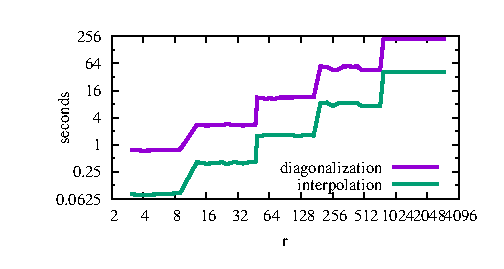
\includegraphics[scale=1]{benchmarks/graphe-101.eps} 


\begin{figure}
\label{fig:exp:uni}
%\resizebox{\columnwidth}{!}{\input{graphe-101}}
\caption{Comparaison entre les phases d'initialisations et la phase d'interpolation pour une courbe définie sur $\mathbb{F}_{101}$ pour $r$ croissant. La courbe est en échelle logarithmique.}
\end{figure}


On a donc regroupé dans la figure~\ref{fig:exp:uni} les deux premières parties
qui sont en fait du précalcul dont le calcul de bases horiontales et comparé 
cela avec la troisième partie qui représente l'interpolation. On voit donc la 
linéarité en $r$ des temps de calcul. 
Le comportement en escalier observé est tout à fait normal car pour toutes les 
isogénies de degré 
$\frac{\ell^{2k-2}(\ell+1)}{4} \leqslant r \leqslant \frac{\ell^{2k}(\ell+1)}{4}$ 
on a besoin de travailler avec la même taille de $\ell^{k}$ torsion, ainsi pour 
différents $r$ dans cet intervalle on aura les polynômes $A_{a,b}$ et $T$ de 
même degré ce qui fait que la complexité et le temp de calcul sont les mêmes. 
Ceci est une raison 
suffisante pour motiver la recherche du plus petit nombre $\ell$ de Elkies car
alors on aura des paliers plus petits pour l'algorithme. Il pourrait toutefois 
s'avérer que pour un autre nombre de Elkies $\ell'$ plus grand que $\ell$, $r$ 
se trouve à la fin du palier $\frac{\ell'^{2k-2}(\ell+1)}{4} \leqslant r 
\leqslant \frac{\ell'^{2k}(\ell+1)}{4}$, ainsi il serait plus utile de 
travailler avec $\ell'$ plutôt que $\ell$.

Comme l'étape d'interpolation va être répétée $O(r)$ fois alors on compare le 
temps de calcul obtenu pour différentes tailles de corps fini.
On présente donc une première série de tests qui a été réalisé sur des 
courbes qui ont toutes leur $\beta=h=2$, ainsi notre 
algorithme~\ref{alg:cou:ell-adique} a travaillé avec la $2^3$ torsion jusqu'à la 
$2^8$ torsion sur des courbes elliptiques définies sur corps finis de taille 
$p$ allant d'une taille de $7$ bits à $252$ bits.



\begin{figure}
\label{fig:exp:dif}
%\include{graphe-101-149-269}
\caption{Comparaison d'une phase d'interpolation pour $r$ croissant pour différentes courbes définies sur les corps finis $\mathbb{F}_{101}$, $\mathbb{F}_{269}$, $\mathbb{F}_{2^{18}+93 }$, $\mathbb{F}_{2^{30}+669}$, $\mathbb{F}_{2^{62}+189}$ et $\mathbb{F}_{2^{252}+421}$. La courbe est en échelle logarithmique.}
\end{figure}

On observe sur la figure~\ref{fig:exp:dif} que la dépendance en $q$ est plus 
grande que ce à quoi on aurait pu s'attendre d'après la borne théorique, cela 
doit être dû à des détails d'implantation bas-niveau que SageMath ne permet pas
de maîtriser.

\begin{figure}
\label{fig:exp:niv}
%\input{graphe-521}
\caption{Comparaison d'une phase d'interpolation pour $r$ croissant pour différentes courbes définies sur les corps finis $\mathbb{F}_{521}$, $\mathbb{F}_{1033}$ et $\mathbb{F}_{2^{62}+169 }$. La courbe est en échelle logarithmique.}
\end{figure}

La deuxième série de tests montrés sur la figure~\ref{fig:exp:niv} a été réalisé
sur des courbes qui ont toutes leur $\beta=h=3$ définies sur des corps finis de
taille $p$ allant de $9$ bits à $62$ bits, notre algorithme~\ref{alg:cou:ell-adique} a donc utilisé de la 
$2^4$ torsion jusqu'à $2^7$ torsion des courbes elliptiques. On voit ici que comme on a 
$\beta=h=3$ alors contrairement aux précédents tests il n'y a pas de palier où l'on travaille avec la 
$\ell^{3}$ torsion mais directement avec la $\ell^4$ torsion, car il est 
nécessaire d'avoir $k$ strictement supérieur à $h$.

Le détail des timings pour les 
différentes parties est disponible sur le projet github: 
\url{https://github.com/Hugounenq-Cyril/Two_curves_on_a_volcano}. 
\chapter{Ouverture 1812}
\section{Variante avec un seul sous-groupe cyclique}
Comme proposé par François Morain on pourrait uniquement travailler avec un 
point horizontal au lieu de travailler avec une base horizontale.

Dés lors on devrait fixer $k$ tel que le nombre d'abscisses de points d'ordre 
$\ell^k:$ $\frac{\ell^{k-1}}{2}$ soit strictement plus grand que $2r$.

Pour le calcul du point horizontal d'ordre $\ell^k$ on est tout de même obligé 
de calculer une base diagonale de la $\ell^{h+1}$-torsion et donc de 
travailler dans l'élément $\mathsf{F}_{h+1-\beta}$ de la tour d'extensions 
$\ell$-adiques.

\begin{prop}
Soit $k$ tel que $\ell^k \in O(r)$, alors pour $h<k$ le coût de calcul d'une 
base diagonale de la $\ell^{h+1}$ torsion à l'aide de 
l'algorithme~\ref{alg:ulti:fro} est de:
$O(\mathsf{M}(r\ell^2)r\ell^2\log(\ell)\log(\ell q) \log(r))$.
\end{prop}

\begin{proof}
On rappelle que l'on travaille avec la convention $\alpha \geqslant \beta$, 
avec $\alpha$ et $\beta$ définis comme dans la proposition~\ref{pro:clas:fro}.
Le coût de calcul de la base horizontale est par la proposition~\ref{pro:alg:ulti}:
$O((h+1)(\mathsf{R}(h+1-\beta)+\ell^2 \mathsf{M}(\ell^{h+1-\beta}))+\ell \mathsf{M}(\ell^2)\log(\ell)\log(\ell q))$. 
En bornant $h$ par $k$ on a $\ell^h \in O(r)$ ce qui en utilisant cette
borne et le coût de $\mathsf{R}(i)$ donné par~\cite[chapter 14.5]{vzGJG03} nous 
donne une complexité de :
$O(\mathsf{M}(r\ell^2)r\ell^2\log(\ell)\log(\ell q) \log(r))$.
\end{proof}
On observe donc que dans ce cas-là on a un coût quadratique en $r$ pour le 
calcul d'une base diagonale de la $\ell^{h+1}$ alors que dans le cas de la 
proposition~\ref{pro:full-complexity} on montrait dans la preuve que le coût 
d'une telle opération était quasi-linéaire.

Ensuite on calcule un point horizontal d'ordre $\ell^k$ à l'aide de 
l'algorithme~\ref{alg:hor:poi} qui a un coût de 
$O(\mathsf{R}(k-\alpha) + k\mathsf{R}(h-\alpha+1) + k\ell^2\mathsf{M}(\ell^{h-\alpha+1}))$
d'après la proposition~\ref{pro:alg:hor}, ce qui appliqué à notre cas donne 
une complexité de: $O(r \mathsf{M}(r \ell)\log(\ell)\log(\ell q) \log(r))$.

Pour le calcul du polynôme d'interpolation on utilise des méthodes 
similaires à celles de la section~\ref{sec:interpolation} mais plus proches de 
celles de \cite[§5]{DeFeo11} vu qu'ici on travaille uniquement avec un sous-groupe 
cyclique. En effet on travaille avec le sous-groupe cyclique d'ordre $\ell^k$ 
défini dans la plus petite extension $\ell$-adique: $\mathsf{F}_{k-\alpha}$. 
On a alors au plus $\frac{\ell^{k-1}}{\ell^{k-\alpha}}=\ell^{\alpha-1}$ représentants 
des orbites selon l'action du Frobenius à calculer dans $\mathsf{F}_{k-\alpha}$.
Le calcul de ces représentants a un coût de 
$O(\ell^{\alpha-1}\mathsf{M}(\ell^{k-\alpha})\log(\ell^k))=O(\mathsf{M}(r)\log(r))$ opérations.

Ensuite on doit calculer le polynôme d'interpolation en appliquant le résultat
 de la proposition~\ref{prop:interpol} avec $t \in \Theta(r)$, $s=\ell^{\alpha-1}$, 
 $n=k-\alpha$ on obtient un complexité de 
 $O(\mathsf{M}(\ell^2r)\log(\ell)\log(r))$qui est l'étape dominante dans les
 étapes \ref{alg:cou-ell:ord} à \ref{alg:cou-ell:Cauchy} de 
 l'algorithme~\ref{alg:cou:ell-adique}.

Ainsi pour le calcul du polynôme on doit répéter l'étape d'interpolation 
$\ell^{k-1}$ fois ce qui nous donne un coût total de: 
$O(r\mathsf{M}(\ell^2r)\log(\ell)\log(r))$ opérations sur $\mathbb{F}_q$.

\begin{prop}
Soit $\ell$ un nombre de Elkies tel que $\ell^h<r$ alors le coût de la 
variante de l'algorithme de Couveignes $\ell$-adique présenté dans 
l'algorithme~\ref{alg:app:cou:var} 
est de: 
$O(r\mathsf{M}(\ell^2r)\log(\ell)\log(r))$ opérations sur $\mathbb{F}_q$.
\end{prop}

Le coût de cette variante de Couveignes $\ell$-adique a donc une complexité de
$O(\mathsf{M}(r\ell^2)r\ell^2 \log(r) \log(\ell) \log(\ell q)$ qui est donc un 
peu plus élevé que le résultat obtenu à la 
proposition~\ref{pro:full-complexity}, la différence notable c'est qu'ici la 
complexité est dominée par la phase de calcul d'une base diagonale de la 
$\ell^{h+1}$ torsion et non pas par la partie interpolation de l'algorithme qui
peut être répétée jusqu'à $\Theta(r)$ fois.


On pourrait penser à utiliser l'algorithme de Couveignes $\ell$-adique avec une
approche multimodulaire de façon similaire à un théorème des restes chinois, 
c'est à dire pour différents nombres de Elkies $\ell_1, \ell_2, \ell_3, \dots, 
\ell_{n}$, pour une isogénie de degré $r$ premier avec tous les $\ell_i$ on 
calcule des bases horizontales de la $\ell_i^{k_i}$ torsion, on peut alors 
travailler avec les deux groupes de points:
\begin{itemize}
\item $\cup_{i=1}^n \mathbb{Z}/\ell_i^{k_i} \mathbb{Z} \times \mathbb{Z}/\ell_i^{k_i} \mathbb{Z}$, 
\item $\prod_{i=1}^n \mathbb{Z}/\ell_i^{k_i} \mathbb{Z} \times \mathbb{Z}/\ell_i^{k_i} \mathbb{Z} $.
\end{itemize}
On va détailler chacune de ces approches dans les deux sous-sections qui suivent.

\section{Aprroche avec le groupe de points isomorphe à $\cup_{i=1}^n \mathbb{Z}/\ell_i^{k_i} \mathbb{Z} \times \mathbb{Z}/\ell_i^{k_i} \mathbb{Z}$}
La première approche est de considérer l'ensemble de points $S$ isomorphe à: 
$\cup_{i=1}^n \mathbb{Z}/\ell_i^{k_i} \mathbb{Z} \times \mathbb{Z}/\ell_i^{k_i} \mathbb{Z} $,
avec les $\ell_i$ tous des nombres premiers de Elkies, dés lors il faut fixer comme 
condition  $\sum_{i=1}^n\ell_i^{2k_{i}-2}(\ell_i+1)>4r$
afin que le polynôme d'interpolation que l'on cherche à construire puisse 
définir la fraction rationnelle $F$ candidate pour représenter la $r$-isogénie 
$\phi$ que l'on veut calculer. 
L'avantage de cette approche est que bien que l'on soit obligé de travailler
sur différentes tours d'extensions $\ell$-adiques, on a pas besoin de 
travailler avec des composita de tours d'extensions $\ell$-adiques.

Détaillons comment on procède, la méthode est restranscrite dans 
l'algorithme~\ref{alg:cou:mult-adique:short}.%, 
%l'algorithme~\ref{alg:cou:mult-adique} détaillant un peu plus 
%l'algorithme~\ref{alg:cou:mult-adique:short} est disponible en annexe.

\begin{algorithm}
\caption{\label{alg:cou:mult-adique:short} Algorithme de Couveignes $\ell$-adique avec approche muti-modulaire.}
\begin{algorithmic}[1]
\REQUIRE $E,E'$: deux courbes elliptiques $r$-isogènes ordinaires situées au niveau $h_i-e_i$ d'un volcan de $\ell_i$-isogénies avec cratère cyclique.
\ENSURE $\phi$ la $r$-isogénie qui relie $E$ à $E'$.
% \STATE Calcul $(P_1,Q_1)$, a basis of $E[\ell]$
\STATE Calcul des $k_i$ tel que $\sum_{i=1}^n\ell_{i}^{2k_{i}-2}(\ell_{i}+1)>4r$;
\FOR{$i=1$ à $n$}
\STATE \label{alg:mult-ell:bhor} Calcul de $(\color{red}P_{\lambda,i}\color{black},\color{blue}Q_{\mu,i}\color{black}),(\color{red}P'_{\lambda,i}\color{black},\color{blue}Q_{\mu,i}'\color{black})$ bases (partiellement) horizontales de $E[\ell_i^{k_i}],E'[\ell_i^{k_i}]$ à l'aide de l'algorithme~\ref{alg:ulti:fro} et de l'étape~\ref{alg:cou-ell:bhor} de l'algorithme~\ref{alg:cou:ell-adique};
\STATE \label{alg:mult-ell:rep} Calcul des liste de représentants $L_i,L_i'$ des orbites de points d'ordre $\ell_i^{k_i}$ sous l'action de $\pi$;
\ENDFOR
\FOR{$M \in \mathsf{diag}(a,b)$  avec $a,b \in \left( \mathbb{Z}/\prod_{i=1}^n\ell_i^{k_i}\mathbb{Z} \right)^*$}
\FOR{$M_i \in \mathsf{diag}(a_i,b_i)$  avec $a=a_i \bmod \ell_i^{k_i},b=b_i \bmod \ell_i^{k_i}$}
\STATE \label{alg:mult-ell:ord} Actualisation de la liste des représentants $L_i'$ en $L'_{a,b,i}$ afin de respecter la correspondance induite par le choix de $M_i$;
\STATE \label{alg:mult-ell:int} Calcul des des polynômes $A_{a,b,i}$ et $T_i$ par les méthodes décrites dans la section~\ref{sec:interpolation};
\ENDFOR
\STATE Calcul des polynômes $A_{a,b}$ et $T$ à l'aide d'un théorème des restes chinois appliqué sur tous les $A_{a,b,i}$ et $T_i$;
\STATE \label{alg:mult-ell:Cauchy} Calcul de la fraction rationnelle $F=A_{a,b} \bmod T$ à l'aide d'une interpolation de Cauchy;
\IF{$\mathsf{Test}(F)$}
\RETURN $F$
\ENDIF
\ENDFOR 
\end{algorithmic}
\end{algorithm}

Les étapes \ref{alg:mult-ell:bhor} à \ref{alg:mult-ell:rep} de 
l'algorithme~\ref{alg:cou:mult-adique:short} qui calculent une base (partiellement) 
horizontale et des représentants des orbites de points (partiellement) 
horizontaux d'ordre $\ell_i^{k_i}$ sous l'action du Frobenius sont faites en 
parallèle sur chacune des tours d'extension $\ell_i$-adiques, les méthodes 
utilisées sont les mêmes que celles dans l'algorithme~\ref{alg:cou:ell-adique}.
Par la proposition~\ref{pro:par:iso} et le corollaire~\ref{cor:par:hor} on sait
 que pour tout $i$ l'action de $\phi$ sur une base
$(\color{red}P_{\lambda,i}\color{black},\color{blue}Q_{\mu,i}\color{black})$
 (partiellement) horizontale de $E[\ell_i^{k_i}]$ peut être représentée de la façon suivante:
$
\left(\begin{smallmatrix}
\color{red} P'_{\lambda,i} \\
\color{blue} Q'_{\mu,i} \color{black}
\end{smallmatrix} \right)= \left(\begin{smallmatrix}
a_i & 0 \\
0 & b_i\end{smallmatrix} \right)
\left(\begin{smallmatrix}
\color{red} P_{\lambda,i} \\
\color{blue} Q_{\mu,i} \color{black} \end{smallmatrix} \right)$
avec $ a_i,b_i \in \left( \mathbb{Z}/\ell_i^{k_i}\mathbb{Z} \right)^*$ et 
$(\color{red}P'_{\lambda,i}\color{black},\color{blue}Q'_{\mu,i}\color{black})$
base (partiellement) horizontale de $E'[\ell_i^{k_i}]$.

On définit à l'aide du théorème des restes chinois deux coefficients $a,b \in 
\left( \mathbb{Z}/\prod_{i=1}^n\ell_i^{k_i} \mathbb{Z} \right)^*$ tels que 
$a=a_i \bmod \ell_i^{k_i}$ et $b=b_i \bmod \ell_i^{k_i}$ pour $i\in [1,n]$.
On calcule ensuite pour chaque couple de coefficients 
$(a,b) \in (\mathbb{Z}/\prod_{i=1}^n\ell_i^{k_i}\mathbb{Z})^*$ à l'aide des 
méthodes de la section~\ref{sec:interpolation} appliquées
à chacune des tours d'extensions $\ell_i$-adiques les polynômes 
d'interpolation $A_{a,b,i}$ et $T_i$ définis dans $\mathbb{F}_q$.
 On applique alors le théorème des restes chinois à ces polynômes pour obtenir 
 les polynômes $A_{a,b},T \in \mathbb{F}_q[x]$ tels que:
 \[
A_{a,b}=A_{a,b,i} \bmod T_i \text{ pour tout } i \in [1,n] \text{ et } \quad T=\prod_{i=1}^nT_i 
 \]
On fait le calcul de la fraction rationnelle $F=A_{a,b} \bmod T$ à l'aide d'une
interpolation de Cauchy. On teste si celle-ci est bien une $r$-isogénie,
si cela n'est pas le cas alors on recommence avec d'autres coeffcients $a,b \in 
(\mathbb{Z}/\prod_{i=1}^n\ell_i^{k_i} \mathbb{Z})^*$.
%\newline

\paragraph{Analyse du coût}
{Une telle approche a forcément des coûts de pré-calcul (pour le calcul des bases 
horizontales et des représentants) plus faibles que notre approche dans 
l'algorithme~\ref{alg:cou:ell-adique}. De même dans la boucle que l'on effectue
 pour chaque choix de coefficients $a,b \in (\mathbb{Z}/\prod_{i=1}^n\ell_i^{k_i} \mathbb{Z})^*$
le calcul des polynômes $A_{a,b,i}$ et $T_i$ définis dans $\mathbb{F}_q$ est 
inférieur au calcul de $A_{a,b}$ et $T$ à l'étape~\ref{alg:cou-ell:int} de 
l'algorithme~\ref{alg:cou:ell-adique} cependant le coût de calcul de 
l'interpolation de Cauchy  est de $O(\mathsf{M}(r)\log(r))$ par
 \cite[Théorème 7.5]{algeff17}. Sachant que l'on doit répéter en moyenne cette 
boucle pour tous les $a,b$ possibles appartenant à $(\mathbb{Z}/\prod_{i=1}^n\ell_i^{k_i} \mathbb{Z})^*$
 le coût d'un tel algorithme est minoré par $\Omega(\prod_{i=1}^n\ell_i^{2k_i-2}
 \mathsf{M}(r)\log(r))$ et donc en particulier par $\Omega(r\mathsf{M}(r)
 \log(r))$. 

Une telle approche serait bien évidemment meilleure que 
l'algorithme~\ref{alg:cou:ell-adique} si l'on avait un moyen de préciser si un 
polynôme $A_{a,b,i_0}$ était correct sans connaître la valeur des autres 
$A_{a,b,i}$ dans un cas comme celui-ci on aurait à tester 
$\sum_{i=1}^n \ell_i^{2k_i-2} \in \Theta(r)$ choix possibles pour le polynôme 
d'interpolation, comme dans l'algorithme~\ref{alg:cou:ell-adique}.

Le principal inconvénient de cette approche 
c'est que l'on fixe comme condition sur les $k_i: \sum_{i=1}^n\ell_i^{2k_{i}-2}(\ell_i+1)>4r$
à cause du théorème des restes chinois à appliquer sur tous les $A_{a,b,i}$. 
On voudrait dés lors travailler avec des $k_i$ sur lesquels on aurait comme 
condition nécessaire: $\prod_{i=1}^n\ell_i^{2k_{i}-2}(\ell_i+1)>4r$
c'est ce que l'on va aborder dans la seconde approche.}

\section{Approche avec le groupe de points isomorphe à $\prod_{i=1}^n \mathbb{Z}/\ell_i^{k_i} \mathbb{Z} \times \mathbb{Z}/\ell_i^{k_i} \mathbb{Z} $}
Ainsi dans cette approche on veut travailler avec des points d'ordre 
$\prod_{i=1}^{n} \ell_i^{k_i}$ qui arrivent à porter l'informations donnée par 
les  bases (partiellement) horizontales 
$(\color{red}P_{\lambda_i}\color{black},\color{blue}Q_{\mu_i}\color{black})$ de 
$E[\ell_i^{k_i}]$ avec $\ell_i$ un nombre premier de Elkies, pour faire cela on
a besoin de définir quelques notions. On
va supposer sans perte de généralités que les $k_i$ pour $i \in [1,n]$ sont 
fixés tels que l'on ait $\prod_{i=1}^{n} \ell_i^{2k_i-2}(\ell_i+1)>4r$.

\subsection{Construction de compositas d'extensions $\ell_i$-adiques}
\label{sub:con:com}
\todo{Ajouter notations dans la liste de nomenclatures}

Cette partie s'appuie sur la construction de compositum à partir d'une idée de
%originale de \cite{BrawleyCarlitz87} reprise dans
\cite{DeFeoDoliskaniSchost14} qui donne le moyen de calculer à un coût quasi 
linéaire le changement de représentation d'éléments du compositum. On montre 
donc ici quelques résultats sur une telle construction appliquée à des tours 
d'extensions $\ell_i$-adiques. Afin de ne pas surcharger la lecture de ce 
document de nombreuses preuves étant l'adaptations de techniques présentées 
dans le chapitre~\ref{cha:tour} elles sont présentées dans l'annexe.

Soient $\ell_1, \dots, \ell_n$ $n$ nombres premiers distincts, 
on va supposer dans le reste de ce document que les différentes tours 
d'extensions $\ell_i$-adiques sont définies comme dans le 
chapitre~\ref{cha:tour} dont on note les éléments 
$\mathbb{F}_q \subset \mathsf{F}_{(i,0)} \subset \dots \subset  \mathsf{F}_{(i,j)}$ 
ont chacune des degrés $d_i=[\mathsf{F}_{(i,0)}:\mathbb{F}_q]$ qui lorsqu'ils 
ne sont pas égaux à $1$ doivent être premiers entre eux.

On veut donc tout d'abord définir un compositum de tours d'extensions 
$\ell_i$-adiques, en particulier on veut calculer un compositum qui contient 
tous les éléments des tours d'extensions $\ell_i$-adiques suivant:
$\mathsf{F}_{(1,n_1)}, \dots \mathsf{F}_{(n,n_n)}$. On suppose de plus que les
$\ell_i$ sont ordonnés de telle sorte que pour tout $i \in [2,n]$ 
$\prod_{j=1}^{i-1}d_j\ell_j^{n_j} \geqslant d_i\ell_i^{n_i}$.

On introduit un objet nécesaire à la construction de compositum.
\begin{defi}
Soient $P$ un polynôme unitaire de degré $\deg(P)$ de racines $r_i$ pour 
$i \in [1,\deg(P)]$, $Q$ un polynôme unitaire de degré $\deg(Q)$ de racines 
$s_j$, tels que $P$ et $Q$ aient des racines distinctes et des degrés $\deg(P),
\deg(Q)$ premiers entre eux, alors on définit $R$ le \emph{produit composé} 
comme étant le polynôme de degré $\deg(P)\deg(Q)$ unitaire et de racines 
$r_is_j$ avec $i \in [1,\deg(P)], j \in [1,\deg(Q)]$. On note $R= P\odot Q$.  
\end{defi}
On peut alors montrer comment on construit un compositum à l'aide de la 
proposition suivante: 
\begin{prop}
\label{pro:init:com}
Soient $\ell_1$ un nombre premier, $P$, $Q$ deux 
polynômes unitaires irréductibles de degré $d_1\ell_1^{n_1}$ et $\deg(Q)$ 
premiers entre eux tels que $\mathbb{F}_q[x]/\langle P \rangle \cong 
\mathsf{F}_{(1,n_1)}$ le $n_1$ ème élément de la tour d'extensions 
$\ell_1$-adique vu dans le chapitre \ref{cha:tour}, $\mathbb{F}_q[y]/\langle Q 
\rangle$ une extension degré $\deg(Q)$ de $\mathbb{F}_q$.
 Soit $R=P\odot Q$  le produit composé de $P$ et $Q$, alors 
 $\mathbb{F}_q[z]/\langle R \rangle$ est un corps fini de taille 
 $q^{d_1\ell_1^{n_1}\deg(Q)}$ et est isomorphe à $\mathbb{F}_q[x,y]/
 \langle P,Q \rangle$.
\end{prop}

\begin{proof}
Voir \cite[Theorem 2]{BrawleyCarlitz87}
\end{proof}


On peut alors définir les composita dans notre cas particulier.
\begin{defi}
\label{def:con:com}
On note $\mathbb{K}_1$ le corps $\mathsf{F}_{(1,n_1)}$. Soit $i \in [1,n-1]$ 
supposons que $\mathbb{K}_{i}$ est défini, alors à 
l'aide de la proposition~\ref{pro:init:com} $\mathbb{K}_{i+1}$ est défini comme
 le composita de $\mathbb{K}_i$ et $\mathsf{F}_{(i+1,n_{i+1})}$.
\end{defi}
\begin{rem}
Ici le cas où l'on aurait $d_i=d_j$ pour $i<j$ entraîne dés lors que l'on a pas
les conditions pour appliquer la proposition~\ref{pro:init:com}. \todo{voir si on peut pas améliorer cette remarque} 
En pratique il est raisonnable de penser que l'on a pas $d_i=d_j=1$ car cela 
voudrait dire que l'on a $E[\ell_i \ell_j] \subset E(\mathbb{F}_q)$ 
\end{rem}

(voir par exemple 
%\cite{Schost15} pour un contexte) \todo{surement plus du tout utile}
\begin{nota} Afin de simplifier les notations on va 
 noter $m_i=\prod_{i=j}^nd_j\ell_j^{n_j}/d_i\ell_i^{n_i}$ et 
 $p_{i}=\prod_{j=1}^{i}d_j\ell_j^{n_j}$, en particulier $p_{i}$ est le 
 degré du composita $\mathbb{K}_i$ comme extension de $\mathbb{F}_q$, par 
 ailleurs on pose $p_0=1$.
%$m_i = \overset{n}{\underset{j \neq i}{\underset{j = 0}{\prod \ell_j^{k_j}}}}$
\end{nota}

Il reste à voir en pratique le coût de la construction d'un tel composita pour 
cela on se sert du résultat suivant issu de \cite[Theorem 1]{BostanFlajoletSalvySchost06}

\begin{prop}[Bostan Flajolet Salvy Schost]
\label{pro:comp:prod}
Soient $f$ et $g$ deux polynômes unitaires de $\mathbb{F}_q[z]$ de degré $m$ et $n$, on note alors $D=mn$
\begin{enumerate}
\item Pour $p$, la caractéristique de $\mathbb{F}_q$, tel que $p>D$ alors le produit composé de $f$ et $g: f \odot g$ peut être calculé à l'aide de  $O(\mathsf{M}(D))$ opérations sur $\mathbb{F}_q$,
\item Pour $p$, tel que $p<D$ et $p$ plus grand que la multiplicité des racines de $f \odot g$, alors $f \odot g$ peut être calculé à l'aide de $O(p\mathsf{M}(\frac{D}{p})\log(\frac{D}{p})+\mathsf{M}(D))$
\end{enumerate}
\end{prop}

\begin{proof}
Voir \cite{BostanFlajoletSalvySchost06}.
\end{proof}

\begin{prop}
\label{pro:con:comp}
Le coût de construire $\mathbb{K}_n$
\begin{enumerate}
\item pour $p$, la caractéristique de $\mathbb{F}_q$, tel que $p>p_n$
est majoré par $O(n\mathsf{M}(p_n))$;
\item pour $p$ tel que $p<p_n$ est majoré par 
$O(n(p\mathsf{M}(\frac{p_n}{p})\log(\frac{p_n}{p})+\mathsf{M}(p_n)))$.
\end{enumerate}
\end{prop}

\begin{proof}
La construction des différentes tours $\ell_i$-adiques se fait à l'aide de 
$O(d_i\mathsf{M}(d_i)\log(d_i)\log(d_iq)+\mathsf{M}(\ell_i)\log(\ell_i)+d_i^2)$ 
opérations sur $\mathbb{F}_q$ par le théorème~\ref{thm:init:tow}, on peut 
majorer cela grossièrement par 
$O(n \max_i(\ell_i\mathsf{M}(\ell_i)\log(\ell_i)\log(\ell_iq))$.
On va alors simplifier l'analyse de complexité en ne considérant que les deux 
cas $p>p_n$ et $p<p_n$.

On travaille donc tout d'abord avec le premier cas, le plus favorable, $p>p_n$.
Supposons que $\mathbb{K}_i$ ait été construit alors calculons le coût de 
construire $\mathbb{K}_{i+1}$, on applique alors la 
proposition~\ref{pro:comp:prod} avec deux polynômes irréductibles de degré 
$p_i$ et $d_{i+1}\ell_i^{n_i}$ cela coûte $O(\mathsf{M}(p_i+1))$ opérations sur
$\mathbb{F}_q$.Ainsi en majorant grossièrement le coût de cette étape par 
$O(\mathsf{M}(p_n))$ le coût de construction du compositum $\mathbb{K}_n$ 
est majoré par $O(n\mathsf{M}(p_n))$.

On travaille maintenant avec le second cas, le moins favorable, $p<p_n$.
Supposons que $\mathbb{K}_i$ ait été construit alors calculons le coût de 
construire $\mathbb{K}_{i+1}$, on applique alors la 
proposition~\ref{pro:comp:prod} avec deux polynômes irréductibles de degré 
$p_i$ et $d_{i+1}\ell_i^{n_i}$ tels que $p>p_n$ alors le calcul de 
$\mathbb{K}_i$ coûte 
$O(p\mathsf{M}(\frac{p_i}{p})\log(\frac{p_i}{p})+\mathsf{M}(p_i))$
opérations sur $\mathbb{F}_q$. Ainsi en majorant grossièrement le coût de cette
étape par $O(p\mathsf{M}(\frac{p_n}{p})\log(\frac{p_n}{p})+\mathsf{M}(p_n))$
le coût de construction du compositum $\mathbb{K}_n$ est majoré par 
$O(n(p\mathsf{M}(\frac{p_n}{p})\log(\frac{p_n}{p})+\mathsf{M}(p_n)))$.
\end{proof}


\todo{changer tous les composita en compositum}

 Comme motivé dans la sous sous section précédente~\ref{sub:TRCE:cou} on peut 
 calculer les points (partiellement) horizontaux sur les volcans de 
 $\ell_i$-isogénies à l'aide des méthodes vues dans le 
 chapitre~\ref{cha:con:poi}, on doit alors ensuite les exprimer dans le
 compositum afin de les utiliser pour le théorème des restes chinois.
  
 Voyons à quel coût on peut exprimer un élément de $\mathsf{F}_{(i,n_i)}$ dans 
 $\mathbb{K}_n=\otimes_{i=1}^n\mathsf{F}_{(i,n_i)}$. On a donc 
 besoin du résultat suivant issu de \cite[Theorem 1]{DeFeoDoliskaniSchost14}
 \begin{prop}[De Feo, Doliskani, Schost]
 \label{pro:com:inj}
 Soient $i \in [2,n] $ $P,Q$ deux polynômes irréductibles unitaires de degrés 
 premiers entre eux $d_i\ell_i^{n_i}$ et $p_{i-1}$ avec
   $\mathbb{F}_q[x]/\langle P \rangle \cong \mathsf{F}_{(i,n_i)}$ et 
   $\mathbb{F}_q[y]/\langle Q \rangle \cong \mathbb{K}_{i-1}$. Alors le 
   plongement d'un élément de $\mathsf{F}_{(i,n_i)} $  dans $\mathbb{K}_{i}$ a un
   coût de 
   $O(d_i\ell_i^{n_i}\mathsf{M}(p_{i-1})+p_{i-1}\mathsf{M}(d_i\ell_i^{n_i}))$ 
   opérations sur $\mathbb{F}_q$. La descente d'un élémént de $\mathbb{K}_{i} $
   vers un élément de $\mathsf{F}_{(i,n_i)}$  a un coût identique. 
   De même le plongement d'un élément de $\mathbb{K}_{i-1}$ dans 
   $\mathbb{K}_{i}$ aini que la descente d'un élément de $\mathbb{K}_{i}$ dans 
   $\mathbb{K}_{i-1}$ ont le même coût.
 \end{prop}

 \begin{proof}
 Voir \cite{DeFeoDoliskaniSchost14}.
\end{proof}  

On voit qu'avec la construction de la définition~\ref{def:con:com} on connaît 
seulement le polynôme, avec la notation de la proposition~\ref{pro:com:inj}, $Q$
qui définit l'extension $\mathbb{K}_{i-1}$ de degré $p_{i-1}$ de 
$\mathbb{F}_q$. Ainsi pour connaître tous les polynômes qui définissent les 
extensions de degé $\frac{\prod_{i=1}^{n}d_i\ell_i^{n_i}}{d_j \ell_j^{n_j}}$ de
$\mathbb{F}_q$ on doit changer l'ordre des $\ell_i$ dans la construction de la 
définition~\ref{def:con:com}, on doit donc calculer $n$ constructions 
différentes de composita pour pouvoir calculer le plongement de tous les 
$\mathsf{F}_{(i,n_i)}$ dans $\mathbb{K}_{n}$ cela a un coût majoré par 
$O(n^2(p\mathsf{M}(\frac{p_n}{p})\log(\frac{p_n}{p})+\mathsf{M}(p_n)))$ 
opérations sur $\mathbb{F}_q$ d'après la proposition~\ref{pro:con:comp}.

 On sera ammené à multiplier des polynômes à coefficients dans un 
 compositum, ainsi on a besoin du résultat suivant.

 \begin{prop}
 \label{pro:mul:com}
 La multiplication et la division euclidienne de polynômes de degré au plus $d$
 à coefficients dans $\mathbb{K}_{n} \cong \mathbb{F}_q[x]/ \langle P \rangle$
 avec $P$ un polynôme irréductible de degré $p_n$ est de $O(\mathsf{M}(p_nd))$ 
 opérations sur $\mathbb{F}_q$.
 \end{prop} 
 
 \begin{proof}
 La preuve est la même que celle de la proposition~\ref{pro:mult:pol}.
 \end{proof}
 
 On sera aussi amené à trouvé une racine d'un polynôme de degré $d$ à 
 coefficients dans un compositum $\mathbb{K}_n$, d'où le résultat suivant:
 
\begin{prop}
\label{pro:rac:com}
 Le coût de calcul de racines de polynômes de degré $d$ à coefficients dans un 
 compositum $\mathbb{K}_{n} \cong \mathbb{F}_q[x]/ \langle P \rangle$
 avec $P$ un polynôme irréductible de degré $p_n$ a un coût espéré de 
 $O(p_n \mathsf{M}(p_nd)\log(d)\log(dq))$ opérations sur $\mathbb{F}_q$.
\end{prop}
 
\begin{proof}
Pour obtenir ce résultat on applique les résultats de \cite[Chapter 14.5]{vzGJG03}.
\end{proof}

\begin{nota}
On va noter par $R(i,j)$ le coût de trouver la racine d'un polynôme de degré 
$i$ à coefficients dans le compositum $\mathbb{K}_j$, donc 
$R(i,j)=O(p_j \mathsf{M}(p_ji)\log(i)\log(iq))$.
\end{nota}

Maintenant voyons un résultat qui nous permet de changer la 
représentation d'un élément de $\mathbb{K}_i$ afin de le représenter comme un 
élément de $\mathbb{K}_{i-1} \otimes \mathsf{F}_{(i,n_i)}$. 

\begin{prop}
\label{pro:iso:fie}
Soient $i \in [1,n]$, $P(x),Q(y)$ deux polynômes irréductibles unitaires de degrés 
$d_i\ell_i^{k},p_{i-1}$ premiers entre eux à coefficients dans $\mathbb{F}_q$
qui définissent $\mathbb{F}_q[x]/\langle P \rangle \cong \mathsf{F}_{(i,k)}$,
$\mathbb{F}_q[x]/\langle Q \rangle \cong \mathbb{K}_{i-1}$. Soit $R=P \odot 
Q$ le produit composé de $P$ et $Q$ alors l'application de l'isomorphisme:
\begin{equation*}
\begin{alignedat}{1}
\varrho : \mathbb{F}_q[x,y]/\langle P, Q \rangle & \rightarrow \mathbb{F}_q[z]/\langle R \rangle \\
xy & \mapsto z
\end{alignedat}
\end{equation*}
a un coût de:
\begin{enumerate}
\item $O((d_i\ell_i^{k})^2\mathsf{M}(p_{i-1}))$ opérations sur $\mathbb{F}_q$
 et l'application de l'inverse de $\varrho$ a un coût de 
 $O(\mathsf{M}(d_i\ell_i^{k}p_{i-1})p_{i-1}^{1/2}+\mathsf{M}(d_i\ell_i^{k})p_{i-1}^{(\omega+1)/2})$ 
opérations sur $\mathbb{F}_q$ lorsque 
$d_i\ell_i^{k} \leqslant p_{i-1}$,
\item $O(p_{i-1}^2\mathsf{M}(d_i\ell_i^{k}))$ opérations sur $\mathbb{F}_q$ 
et l'application de l'inverse de $\varrho$ a un coût de 
$O(\mathsf{M}(p_{i-1}d_i\ell_i^{k})(d_i\ell_i^{k})^{1/2}+\mathsf{M}(p_{i-1})(d_i\ell_i^{k})^{(\omega+1)/2})$ 
opérations sur $\mathbb{F}_q$ lorsque $d_i\ell_i^{k} \geqslant p_{i-1}$.
\end{enumerate}
\end{prop}
\todo{on pourrait éventuellement faire un restriction sur les $\ell_i$ pour que cela soit toujours vérifié}
\begin{proof}
Voir \cite{DeFeoDoliskaniSchost14}.
\end{proof}

Ainsi on peut appliquer ce résultat pour calculer le coût du Frobenius avec 
une méhtode similaire à celle du théorème~\ref{thm:frob-ell}
\begin{prop}
\label{pro:fro:com}
Soit $i \in [1,n]$, $P$ un polynôme irréductible de degré $d_i\ell_i^{k}$ avec 
$k \in [1,n_i]$ tel que $\mathsf{F}_{(i,k)}=\mathbb{F}_q[x]/\langle P \rangle$,
$Q$ un polynôme irréductible de degré $p_{i-1}=\prod_{j=1}^{i-1}d_j\ell_j^{k_j}$
tel que $\mathbb{K}_{i-1}=\mathbb{F}_q[y]/\langle Q \rangle$, $R=P \odot Q$ 
tel que  $\mathbb{K}_{i}=\mathbb{F}_q[z]/\langle R\rangle$, alors pour un 
élément $a$ de $\mathbb{K}_{i}$ le coût de calcul de $a$ à une puissance 
$q^{r p_{i-1}}$ est de 
$O(\mathsf{M}(d_i\ell_i^{k}p_{i-1})p_{i-1}^{1/2}+\mathsf{M}(d_i\ell_i^{k})p_{i-1}^{(\omega+1)/2})$ 
opérations dans $\mathbb{F}_q$ avec un 
précalcul qui a un coût booléen de $O(\log(p_{i})\log(\ell_i^{n_i}qd_i))$ et  
de $O( M(d_i) d_i\log(q))$ opérations sur $\mathbb{F}_q$.
\end{prop}

\begin{proof}
Voir la preuve en annexe~\ref{cha:ann:comp}.
\end{proof}


On voit dans cette preuve que le coût de changement de représentation des 
éléments de $\mathbb{K}_i$ vers une représentation de la forme 
$\mathbb{K}_{i-1} \otimes \mathsf{F}_{(i,n_i)}$ est crucial dans le coût total
du Frobenius. En effet si on compare ce résultat avec celui du 
théorème~\ref{thm:frob-ell} on voit l'influence du changement de représentation
à coût nul.

Une adaptation des méthodes de calcul de polynôme d'interpolation décrites dans
la section~\ref{sec:interpolation} à ce contexte est développée en annexe, on
ne retranscrit ici que le résultat final suivant.

\begin{prop}\label{prop:interpol:comp}
  Soit $(v_1,w_1),\dots,(v_s,w_s)$ des paires d'éléments de $\mathbb{K}_n 
  \setminus \mathbb{K}_{n-1}$, $t_i$ le degré des polynômes minimaux de $v_i$, 
  et l'on note  $t=\sum t_i$. 
  Les polynômes
  \begin{itemize}
  \item $T\in \mathbb{F}_q[x]$ de degré $t$ tel que $T(v_i)=0$ pour tout $i$,
    et
  \item $A\in \mathbb{F}_q[x]$ de degré inférieur à $t$ tel que $A(v_i)=w_i$ pour
    tout $i$
  \end{itemize}
  sont calculés avec un coût de
  $O\bigl(\mathsf{M}(t)\log(s) + n\mathsf{M}(t \max_i(d_i\ell_i^{n_i}))(p_{n-1})^{(\omega-1)/2} \max_{i}(\ell_{n-i})\bigr)$ 
  opérations dans $\mathbb{F}_q$ avec un coût de 
  $O(nsM(p_n)p_{n-1}^{(\omega-1)/2})$ opérations dans $\mathbb{F}_q$ pour 
  l'expression des éléments dans le sous-corps de $\mathbb{K}_n$ le plus petit 
  au sens de l'inclusion.
\end{prop}

\begin{proof}
Voir annexe~\ref{cha:ann:comp}.
\end{proof}

\subsection{Théorème des Restes Chinois Elliptique et son application à l'algorithme de Couveignes $\ell$-adique}
\label{sub:TRCE:cou}
\begin{defi}
Soient $\ell_1, \ell_2$ deux nombres premiers distincts, $E$ une courbe 
elliptique. On énonce alors le Théorème des Restes Chinois dans le contexte des
courbes elliptiques comme suit:

Soient $P_1$ un point d'ordre $\ell_1^{k_1}$ de $E$ et $P_2$ un point d'ordre $\ell_2^{k_2}$ de $E$ alors ces deux points sont associés isomorphiquement à un point $P$ d'ordre $\ell_1^{k_1}\ell_2^{k_2}$ tel que $[\ell_1^{k_1}]P=P_2$ et $[\ell_2^{k_2}]P=P_1$.
\end{defi}

Maintenant que l'on a énoncé le théorème des restes chinois pour une courbe elliptique montrons comment on le résoud à l'aide de l'algorithme~\ref{alg:TRC:init}.
\todo{trouver un meilleur nom pour cet algorithme}
\begin{algorithm}
\caption{\label{alg:TRC:init}Calcul de  représentant de $P_1$ dans $E[\mathbb{Z}/\ell_1^{k_1}\ell_2^{k_2}\mathbb{Z}]$ ou TRC simplifié...}
\begin{algorithmic}[1]
\REQUIRE $E$: une courbe elliptique, $\ell_1,\ell_2$ deux nombres premiers distincts, $P_1$ un point d'ordre $\ell_1^{k_1}$.
\ENSURE $P$ un point de $E$ d'ordre $\ell_1^{k_1}\ell_2^{k_2}$  tel que $[\ell_1^{k_1}]P=0_E$ et $[\ell_2^{k_2}]P=P_1$.
% \STATE Calcul $(P_1,Q_1)$, a basis of $E[\ell]$
\STATE \label{alg:TRC:init:div} Calcul de $P'=\mathsf{divise}(P_1,\ell_2^{k_2})$;
\STATE \label{alg:TRC:init:mul} Calcul de $Q=[\ell_1^{k_1}]P'$ un point d'ordre $\ell_2^{k_2}$;
\STATE \label{alg:TRC:init:prim} Calcul de $R$ la pré-image de $Q$ d'ordre $\ell_2^{k_2}$ par $[\ell_1^{k_1}]$;
\RETURN $P'-R$
\end{algorithmic}
\end{algorithm}

\begin{prop}
L'algorithme~\ref{alg:TRC:init} est correct.
\end{prop}

\begin{proof}
Un calcul direct montre que $[\ell_1^{k_1}](P'-R)=Q-Q=0_E$ et 
 $[\ell_2^{k_2}](P'-R)=P_1-0_E$.
\end{proof}

\begin{prop}
La sortie de l'algorithme~\ref{alg:TRC:init} est unique.
\end{prop}

\begin{proof}
Soient $P,S$ deux points d'ordre $\ell_1^{k_1}\ell_2^{k_2}$  obtenus par 
l'algorithme~\ref{alg:TRC:init}  tels que 
$[\ell_2^{k_2}]P=[\ell_2^{k_2}]S=P_1$ et  
$[\ell_1^{k_1}]P=[\ell_1^{k_1}]S=0_E$. Alors on a $[\ell_2^{k_2}](P-S)=0$ et 
$[\ell_1^{k_1}](P-S)=0$ ce qui veut dire que l'ordre de $P-S$ divise à la fois 
$\ell_1^{k_1}$ et $\ell_2^{k_2}$ d'où le résultat. On vérifie donc bien le 
théorème des restes chinois.
\end{proof}

Ainsi une solution du problème des restes chinois pour $P \in E[\mathbb{Z}/
\ell_1^{k_1} \ell_2^{k_2}\mathbb{Z}]$ tel que $\ell_1^{k_1}P=P_2 \in 
E[\ell_2^{k_2}]$ et $\ell_2^{k_2}P=P_1 \in E[\ell_1^{k_1}]$ est donnée par 
$P=Q+R$ avec:
\begin{itemize}
\item $Q$ la sortie de l'algorithme~\ref{alg:TRC:init} qui a pour entrées
$\ell_1^{k_1}, \ell_2^{k_2}$ et $P1$ d'ordre $\ell_1^{k_1}$,
\item  $R$ la sortie de l'algorithme~\ref{alg:TRC:init} qui a pour entrées
$\ell_2^{k_2}, \ell_1^{k_1}$ et $P2$ d'ordre $\ell_2^{k_2}$.
\end{itemize}

\begin{nota}
Introduisons la notation suivante afin d'alléger l'écriture par la suite: 
$\upsilon_n=\prod_{i=1}^n \ell_i^{k_i}$, 
$\vartheta_i=\frac{\upsilon_n}{\ell_i^{k_i}}$.
\end{nota}

\'Enonçons une généralisation du thèorème des restes chinois pour une courbe 
elliptique à $n$ nombres premiers distincts.

\paragraph{Théorème des Restes chinois généralisés sur une courbe Elliptique $E$}
Soient $\ell_1, \dots, \ell_n$ $n$ nombres premiers distincts, les points $P_1 \in E[\ell_1^{k_1}], \dots, P_n \in E[\ell_n^{k_n}]$, alors le théorème des restes chinois revient à déterminer un point $P \in E[\upsilon_n]$ tel que $[\vartheta_{i_0}] P=P_{i_0}$ pour $i_0 \in [1,n]$.

%\overset{n}{\underset{i \neq i_0}{\underset{i = 0}{\prod}}}\ell_i^{k_i}
On présente une généralisation de l'algorithme~\ref{alg:TRC:init} dans 
l'algorithme~\ref{alg:TRC:init:gen} à l'aide de celui-ci on peut résoudre la 
généralisation du théorème des restes chinois d'une courbe elliptique à l'aide 
de l'algorithme~\ref{alg:TRC}. Ces algorithmes sont présentés et leurs 
complexités sont analysées lorsqu'ils sont appliqués sur le compositum 
$\mathbb{K}_n$ dans la sous-section suivante.


Cette approche du théorème des restes chinois a été motivée pour l'appliquer à 
des points (partiellement) horizontaux d'ordre $\ell_i^{k_i}$, la proposition 
suivante montre que cette utilisation du théorème des restes chinois fait sens 
dans le contexte de l'algorithme de Couveignes.

\begin{prop}
\label{pro:par:TRC}
Soient $\ell_1, \ell_2$ deux nombres premiers distincts de Elkies, 
$P_1 \in E[\ell_1^{k_1}]$ un point horizontal d'ordre 
$\ell_1^{k_1}$ et de direction $\lambda_1$, $P_2 \in E[\ell_2^{k_2}]$ un point 
horizontal d'ordre $\ell_2^{k_2}$ et de direction $\lambda_2$. Soit $P \in 
E[\mathbb{Z}/\ell_1^{k_1}\ell_2^{k_2}\mathbb{Z}]$ un point d'ordre 
$\ell_1^{k_1}\ell_2^{k_2}$ tel que $\ell_1^{k_1}P=P_2$ et $\ell_2^{k_2}P=P_1$.
Soit $\phi$ une isogénie de degré $r$ premier avec $\ell_1, \ell_2$ alors 
$\phi(P)$ est tel que
\begin{itemize}
\item $\ell_1^{k_1}\phi(P)$ est un point horizontal d'ordre 
$\ell_2^{k_2}$ et de direction $\lambda_2$,  
\item $\ell_2^{k_2}\phi(P)$ est un point horizontal d'ordre 
$\ell_1^{k_1}$ et de direction $\lambda_1$,
\end{itemize}
\end{prop}

\begin{proof}
Par un raisonnement similaire à la preuve de la proposition~\ref{pro:par:iso}, 
vu que $\phi$ est de degré $r$ premier avec $\ell_1$ et $\ell_2$ alors on a un 
isomorphisme de modules de Tate qui commutent avec le Frobenius.
\end{proof}

Cette proposition se généralise à $n$ nombres de Elkies $\ell_1, \dots, \ell_n$
distincts.

\begin{nota}
Soient $\ell_1, \dots, \ell_n$ $n$ nombres premiers de Elkies distincts, $P$ un
 point d'ordre $\upsilon_n$ de $E$ construit à l'aide du 
 théorème des restes chinois (voir algorithme~\ref{alg:TRC}) tel que 
$[\vartheta_i]P=P_i$ avec $P_i$ des points (partiellement) horizontaux de 
direction $\lambda_i$ et profondeur $e_i$, alors 
on dit que $P$ est de direction $(\lambda_1, \dots, \lambda_n)$ et de 
profondeur $(e_1, \dots, e_n)$. 
\end{nota}

\begin{cor}
Soient $\ell_1, \dots, \ell_n$ $n$ nombres premiers de Elkies distincts et 
premiers avec $r$, $\phi: E \rightarrow E'$ une $r$-isogénie avec $E$ et $E'$ 
qui se situent à une profondeur $e_i$ du cratère du volcan de 
$\ell_i$-isogénies pour $i \in [1,n]$. Alors pour $P$ un
 point d'ordre $\upsilon_n$ de $E$ construit à l'aide de 
l'algorithme~\ref{alg:TRC} tel que $[\vartheta_i]P=P_i$ 
avec $P_i$ des points (partiellement) horizontaux direction $\lambda_i$ et 
profondeur $e_i$, et $P'$ un point d'ordre $\upsilon$ de $E'$ construit à 
l'aide de l'algorithme~\ref{alg:TRC} tel que $[\vartheta_i]P'=P'_i$ avec $P'_i$
des points (partiellement) horizontaux direction $\lambda_i$ et profondeur 
$e_i$ alors $\phi(P) \in \langle P' \rangle$. 
\end{cor}


\begin{rem}
Une application de la proposition~\ref{pro:par:TRC} et de la notation 
précédente est que pour deux courbes elliptiques $E,E'$ $r$-isogènes avec $r$ 
premier avec les nombres premiers $\ell_1, \dots, \ell_n$ un point $P \in E$ 
d'ordre $\upsilon_n$, de direction $(\lambda_1, \dots, \lambda_n)$ et 
profondeur $(e_1, \dots, e_n)$ a pour image par $\phi$ un point $[a]P' \in E'$
avec $a \in (\mathbb{Z}/\upsilon_n \mathbb{Z})^*$ et $P'$ un 
point d'ordre $\upsilon_n$, de direction $(\lambda_1, \dots, \lambda_n)$ et 
profondeur $(e_1, \dots, e_n)$.
\end{rem}
On a donc bien une correspondance entre les points définis à l'aide du Théorème
 des Restes Chinois appliqué à des points (partiellement) horizontaux définis 
 sur deux courbes elliptiques $r$-isogènes avec $r$ premier avec $\ell_1, \dots
 , \ell_n$.
 Maintenant énonçons un résultat qui nous permette de déterminer les 
 représentants d'orbite sous l'action de groupes de Galois en rappelant que 
 l'on note $\mathbb{K}_n=\otimes_{i=1}^{n}\mathsf{F}_{(i,k_i)}$ le composita 
 qui contient tous les éléments $\mathsf{F}_{(i,k_i)}$ des tours d'extensions
 $\ell_i$-adiques construit d'après les restrictions énoncées dans la 
 sous-section~\ref{sub:con:com}.
\begin{prop}
\label{pro:rep:com}
Soit $P$ un point d'ordre $\upsilon_n$ de $E(\mathbb{K}_n)$ obtenu à l'aide 
du théorème des restes chinois appliqué aux points $P_i$ de $E$ d'ordre 
$\ell_i^{k_i}$ tels que l'orbite générée par l'action de 
$\mathsf{Gal}(\mathsf{F}_{(i,k_i)}:\mathbb{F}_q)$ sur $P_i$ soit de taille
 maximale: $d_i\ell_i^{k_i}$.  Alors l'orbite de $P$ selon l'action de 
 $\mathsf{Gal}(\mathbb{K}_n:\mathbb{F}_q)$ est elle aussi de taille maximale:
 $\prod_{i=1}^nd_i\ell_i^{k_i}$.
\end{prop} 

\begin{proof}
Soit $P$ un point de $E$ respectant les conditions de l'énoncé, supposons par 
l'absurde qu'il existe $i_0 \in [1,n]$ et $r_0 \in [1,d_{i_0}\ell_{i_0}^{k_{i_0}}-1]$ 
tel que l'action d'un élément générateur de 
$\mathsf{Gal}(\overset{n}{\underset{j \neq i_0}{\underset{j = 1}{\otimes}}}\mathsf{F}_{(j,k_j)}\otimes \mathsf{F}_{(i_0,k_{i_0})}:\overset{n}{\underset{j \neq i_0}{\underset{j = 1}{\otimes}}}\mathsf{F}_{(j,k_j)})$ 
à la puissance $r_0$ laisse fixe $P$. Par le théorème des restes chinois on 
peut représenter cette action sur $\mathbb{Z}/\ell_{i_0}^{k_{i_0}}\mathbb{Z} 
\times \mathbb{Z}/\vartheta_{i_0}\mathbb{Z}$
à l'aide des deux points $P_{i_0}=[\vartheta_{i_0}]P$  et 
$Q=[\ell_{i_0}^{k_{i_0}}]P$. $Q$ étant défini dans 
$\overset{n}{\underset{j \neq i_0}{\underset{j = 0}{\otimes}}} \mathsf{F}_{(j,k_j)}$ 
il est stable par l'action d'un élément générateur de 
$\mathsf{Gal}(\overset{n}{\underset{j \neq i_0}{\underset{j = 1}{\otimes}}}\mathsf{F}_{(j,k_j)}\otimes \mathsf{F}_{(i_0,k_{i_0})}:\overset{n}{\underset{j \neq i_0}{\underset{j = 1}{\otimes}}}\mathsf{F}_{(j,k_j)})$.
$P_{i_0}$ étant le représentant d'une orbite de taille maximale
sous l'action de $\mathsf{Gal}(\mathsf{F}_{(i_0,k_{i_0})}:\mathbb{F}_q)$ par 
construction alors il ne peut être stable que sous l'action d'un élément 
générateur de 
$\mathsf{Gal}(\overset{n}{\underset{j \neq i_0}{\underset{j = 1}{\otimes}}}\mathsf{F}_{(j,k_j)}\otimes \mathsf{F}_{(i_0,k_{i_0})}:\overset{n}{\underset{j \neq i_0}{\underset{j = 1}{\otimes}}}\mathsf{F}_{(j,k_j)})$
à la puissance $d_{i_0}\ell{i_0}^{k_{i_0}}$, ainsi $r_0$ doit être un multiple 
de $d_{i_0}\ell{i_0}^{k_{i_0}}$.
\end{proof}

\begin{nota}
Soient $\ell_1, \dots \ell_n$ $n$ nombres premier de Elkies, alors on note 
$\epsilon_i$ le nombre de représentants de points d'ordre $\ell_i^{k_i}$ sous 
l'action d'un générateur de $\mathsf{Gal}(\mathsf{F}_{\ell_i^{k_i}}:\mathbb{F}_q)$.
\end{nota}

On voit donc avec la proposition~\ref{pro:rep:com} que pour déterminer des 
représentants pour l'orbite selon l'action du groupe de Galois pour des points 
d'ordre $\upsilon_n$ il suffit de calculer à l'aide du théorème des 
restes chinois tous les points $P$ d'ordre $\upsilon_n$ 
tels que tous les choix possibles de représentants $P_i=[\vartheta_i]P$
par rapport à l'action de $\mathsf{Gal}(\mathsf{F}_{(i,n_i)}:\mathbb{F}_q)$
 aient été effectués. Ainsi le nombre de représentants est
 donc de $\prod_{i=1}^{n} \epsilon_i$. On calcule donc 
 tout d'abord les représentants d'ordre $\ell_i^{k_i}$ dans les tours 
 d'extensions $\ell_i$-adiques, puis on les exprime dans le compositum et enfin
 on applique $\prod_{i=1}^{n} \epsilon_i$ fois le théorème des restes chinois. 
 Pour le théorème des restes chinois on a besoin d'appliquer 
 l'algorithme~\ref{alg:TRC:init:gen} $\sum_{i=1}^{n} \epsilon_i$ fois, une fois
 pour chaque représentant d'ordre $\ell_i^{k_i}$.
  
 On peut dès lors modifier l'algorithme~\ref{alg:cou:ell-adique} de telle sorte
 que l'on travaille avec deux couples de points d'ordre 
 $\prod_{i=1}^n\ell_i^{k_i}$ de même direction au lieu de deux points d'ordre
 $\ell^k$ de même direction comme dans l'algorithme~\ref{alg:cou:ell-adique}.

\subsection{Algorithme de Couveignes $\ell_i$-adique avec le théorème des restes chinois elliptique}

Avant de présenter une analyse des coûts de l'algorithme de Couveignes 
$\ell_i$-adique avec TRC Elliptique utilisant la représentation de composita 
préconisée par \cite{DeFeoDoliskaniSchost14} et développée dans la 
sous-section~\ref{sub:con:com} on présente tout d'abord les coûts d'algorithmes
de Théorème des Restes Chinois Elliptique appliqués sur de telles constructions.

\subsubsection{Coût des algorithmes de calcul de Théorème des Restes Chinois Elliptique}

On présente ici la généralisation de l'algorithme~\ref{alg:TRC:init} avant 
d'analyser sa complexité en reprenant les résultats de la 
sous-section~\ref{sub:con:com}: 


\todo{trouver un meilleur nom pour cet algorithme}
\begin{algorithm}
\caption{\label{alg:TRC:init:gen}Lemme pour Théorème des restes chinois généralisé sur une courbe elliptique }
\begin{algorithmic}[1]
\REQUIRE $E$: une courbe elliptique, $\ell_1, \dots, \ell_n$ $n$ nombres premiers distincts, un point $P_{i_0}$ d'ordre $\ell_i^{k_{i_0}}$ pour $i_0 \in [1,n]$.
\ENSURE $P$ un point de $E$ d'ordre $\prod_{i=1}^n \ell_i^{k_i}$  tel que $[\overset{n}{\underset{i \neq i_0}{\underset{i = 0}{\prod}}}\ell_i^{k_i} ]P=P_{i_0}$ et $[\ell_{i_0}^{k_{i_0}}]P=0_E$.
\STATE $P \leftarrow P_{i_0}$;
% \STATE Calcul $(P_1,Q_1)$, a basis of $E[\ell]$
\STATE \label{alg:TRC:init:gen:div} Calcul de $P'=\mathsf{divise}(P_{i_0},\overset{n}{\underset{j \neq i_0}{\underset{j = 0}{\prod}}}\ell_j^{k_j})$;
\STATE \label{alg:TRC:init:gen:mul} Calcul de $Q=[\ell_{i_0}^{k_{i_0}}]P'$ un point d'ordre $\overset{n}{\underset{j \neq i_0}{\underset{j = 0}{\prod}}}\ell_j^{k_j}$;
\STATE \label{alg:TRC:init:gen:prim} Calcul de $R$ la pré-image de $Q$ d'ordre $\overset{n}{\underset{j \neq i_0}{\underset{j = 0}{\prod}}}\ell_j^{k_j}$ par $[\ell_{i_0}^{k_{i_0}}]$;
\STATE \label{alg:TRC:init:gen:add}$P \leftarrow P'-R$
\RETURN $P$
\end{algorithmic}
\end{algorithm}


\begin{prop}
L'algorithme a une complexité espérée de:
\[
O(n p_{n}\mathsf{M}(p_{n}\ell_{n})\max_i(k_{i}\log(\ell_{i})\log(\ell_{i}q)))
\] 
opérations sur $\mathbb{F}_q$.
\end{prop}

\begin{proof}
Pour le calcul de l'étape~\ref{alg:TRC:init:gen:div} on préconise une 
utilisation de construction de $\mathbb{K}_n$ tel que $\mathbb{K}_1=
\mathsf{F}_{(i_0,k_{i_0})}$ et les 
$\mathbb{K}_i \cong \mathbb{K}_{i-1} \otimes \mathsf{F}_{(i,k_i)}$, dés lors lorsque 
l'on va calculer la division successive par les différents $\ell_i$ on va 
successivement travailler dans les corps 
$\mathbb{K}_2, \mathbb{K}_3, \dots, \mathbb{K}_n$. On suppose sans perte 
de généralités que l'on a $i_0=1$. On décompose 
l'étape~\ref{alg:TRC:init:gen:div} en $n-1$ 
étapes, on appelle $P^{(0)}=P_{1}$ et on définit par récurrence 
$P^{(i+1)}=\mathsf{divise}(P^{(i)},\ell_{i+1}^{n_{i+1}})$, on a alors 
$P^{(i+1)}$ d'ordre $\upsilon_{i+1}$ et défini dans $\mathbb{K}_{i+1}$. 
Calculons le coût de l'étape $i$, on décompose tout d'abord 
$\mathsf{divise}(P^{(i)},\ell_{i+1}^{k_{i+1}})$ à l'aide de $2k_{i+1}$ 
$\ell_{i+1}$-isogénies. Ainsi on pose $P^{(i)}_0=P^{(i)}$ et on définit par 
récurrence $P^{(i)}_{j+1}=\mathsf{divise}(P^{(i)}_{j},\ell_{i+1})$, ce qui nous
 donne $P^{(i+1)}=P^{(i)}_{k_{i+1}}$. On a $P^{(i)}_{j}$ défini dans 
 $\mathbb{K}_i\otimes \mathsf{F}_{(i+1,j)}$ et représenté comme un élément de 
 $\mathbb{K}_{i+1}$ donc le coût de  $\mathsf{divise}(P^{(i)}_{j},\ell_{i+1})$ 
 est $R(\ell_{i+1},p_{i+1})$ c'est à dire 
 $O(p_{i+1} \mathsf{M}(p_{i+1}  \ell_{i+1})\log(\ell_{i+1})\log(\ell_{i+1}q))$
 par la proposition~\ref{pro:rac:com}. Ainsi le coût de calcul de $P^{(i+1)}$ 
 est de 
 $O(k_{i+1}p_{i+1} \mathsf{M}(p_{i+1}  \ell_{i+1})\log(\ell_{i+1})\log(\ell_{i+1}q))$.
 On majore ce coût par $O(p_{n}\mathsf{M}(p_{n}\ell_{n})\max_i(k_{i+1}\log(\ell_{i+1})\log(\ell_{i+1}q)))$
 Il faut alors ajouter le coût de l'expression de $P^{(i+1)}$ dans 
 $\mathbb{K}_{i+2}$ par la proposition~\ref{pro:iso:fie}
 cela a un coût de $O((d_{i+2}\ell_{i+2}^{k_{i+2}})^2\mathsf{M}(p_{i+1}))$,
 ce coût sera alors majoré par le coût de $R(\ell_{i+2},p_{i+2})$ on ne le 
 prend donc pas en compte. 
 Le coût de l'étape~\ref{alg:TRC:init:gen:div} est donc majoré par 
 $O(n p_{n}\mathsf{M}(p_{n}\ell_{n})\max_i(k_{i+1}\log(\ell_{i+1})\log(\ell_{i+1}q)))$. 

Pour le calcul de l'étape~\ref{alg:TRC:init:gen:mul} on décompose la 
multiplication par $\ell_{i_0}^{k_{i_0}}$ en $k_{i_0}$ multiplications par 
$\ell_{i_0}$ que l'on décompose chacune en deux $\ell_{i_0}$-isogénies. $P'$ 
étant défini dans $\mathbb{K}_{n}$ cela coûte 
$O(k_{i_0}(\mathsf{M}(p_n)(\log(p_n)+\ell_{i_0})))$.

L'étape~\ref{alg:TRC:init:gen:prim} se décompose comme 
l'étape~\ref{alg:TRC:init:gen:mul} en $k_{i_0}$ multiplications par 
$\ell_{i_0}$ que l'on décompose chacune en deux $\ell_{i_0}$-isogénies, sauf 
que cette fois-ci on va devoir inverser chacune des $\ell_{i_0}$-isogénies. On 
peut alors soit résoudre des polynômes de degré $\ell_{i_0}$ pour calculer les 
antécédents des $\ell_{i_0}$-isogénies, ou alors on peut déterminer l'action de
la mutliplication par $\ell_{i_0}$ sur les points d'odre $\vartheta_{i_0}$ mais
une telle recherche exhaustive dans l'état actuel où le coût de plongement 
n'est pas négligeable ne rend pas celle-ci intéresante d'un point de vue 
pratique. Ainsi le coût d'une telle étape est de $O(k_{i_0}R(\ell_{i_0},p_n)$ 
soit $O(k_{i_0}p_n\mathsf{M}(p_n\ell_{i_0})\log(\ell_{i_0})\log(\ell_{i_0q}))$ 
opérations sur $\mathbb{F}_q$ auquel il faut ajouter le coût pour identifier la
bonne racine, un moyen rapide de faire cela est d'exprimer les racines dans la 
représentation $\underset{i\neq i_0}\otimes_{i=1}^n \mathsf{F}_{(i,k_i)} \otimes \mathsf{F}_{(i_0,k_{i_0})}$
ce qui a un coût majoré par $O(\mathsf{M}(p_n)(\frac{p_n}{d_{i_0}\ell_{i_0}^{k_{i_0}}})^{(\omega-1)/2})$ par la proposition~\ref{pro:iso:fie} donc un coût total de $O(\ell_{i_0}^2\mathsf{M}(p_n)(\frac{p_n}{d_{i_0}\ell_{i_0}^{k_{i_0}}})^{(\omega-1)/2})$.

L'étape~\ref{alg:TRC:init:gen:add} a elle un coût de $O(\mathsf{M}(p_n)\log(p_n))$.

On voit alors que le coût total de l'algorithme est dominé par 
l'étape~\ref{alg:TRC:init:gen:div}.
\end{proof}

\begin{algorithm}
\caption{\label{alg:TRC} Théorème des restes chinois sur une courbe elliptique}
\begin{algorithmic}[1]
\REQUIRE $E$: une courbe elliptique, $\ell_1,\ell_2, \dots \ell_n$ $n$ nombres premiers distincts, des points $P_i$ d'ordre $\ell_i^{k_i}$ pour $i \in [1,n]$.
\ENSURE $P$ un point de $E$ d'ordre $\upsilon_n$  tel que $[\vartheta_{i_0} ] P=P_{i_0}$ pour $i_0 \in [1,n]$.
% \STATE Calcul $(P_1,Q_1)$, a basis of $E[\ell]$
\STATE $P \leftarrow 0_E$;
\FOR{$i=1$ à $n$}
\STATE $Q$ sortie de l'algorithme~\ref{alg:TRC:init:gen} tel que $\ell_i^{k_i}Q=0$ et $[\vartheta_i]Q=P_i$;
\STATE $P \leftarrow P+Q$; 
\ENDFOR
\RETURN $P$;
\end{algorithmic}
\end{algorithm}

\begin{prop}
L'algorithme~\ref{alg:TRC} a une complexité espérée de 
\[
O(n^2 p_{n}\mathsf{M}(p_{n}\ell_{n})\max_i(k_i\log(\ell_{i})\log(\ell_{i}q))) 
\]
opérations sur $\mathbb{F}_q$.
\end{prop}

 On peut désormais voir dans quelle mesure la représentation
 de compositum avec une méthode telle que celle préconisée 
 dans~\cite{DeFeoDoliskaniSchost14} nous permet d'avoir des résultats 
 similaires sur les optimisations de calcul dues à la construction des tours 
 d'extension $\ell$-adiques utilisées pour 
 l'algorithme~\ref{alg:cou:ell-adique} dont on présente une modification et une
 analyse dans la sous-sous-section suivante. 


\subsubsection{Coût total de l'algorithme de Couveignes $\ell_i$-adique avec le théorème des restes chinois elliptique}
Nous avons abordé dans la sous-sous-section~\ref{sub:TRCE:cou} l'intérêt 
d'utiliser un théorème des restes chinois sur une courbe elliptique par rapport
à l'algorithme de Couveignes. En effet on a vu qu'un point construit à l'aide 
du théorème des restes chinois elliptique appliqué à des points $P_i,Q_i$ 
(partiellement) horizontaux de directions $\lambda_i,\mu_i$  d'ordre 
$\ell_i^{k_i}$, avec $r, \ell_i$ tous premiers entre eux, 
était mis en correspondance avec un autre point de même direction.
Ainsi avec deux bases de points (partiellement) horizontaux $(\color{red}P_{\lambda_1,
 \dots, \lambda_n}\color{black},\color{blue}Q_{\mu_1, \dots, 
 \mu_n}\color{black}),(\color{red}P'_{\lambda_1, \dots, \lambda_n}\color{black}
 ,\color{blue}
 Q'_{\mu_1, \dots, \mu_n}\color{black})$ de $E[\prod_{i=1}^n\ell_i^{k_i}]$ et 
 $E'[\prod_{i=1}^n\ell_i^{k_i}]$ l'action de la $r$-isogénie peut être 
 représentée de la façon suivante:  
 \begin{equation*}
\left(
\begin{matrix}
\color{red} P'_{\lambda_1,
 \dots, \lambda_n} \\
\color{blue} Q'_{\mu_1, \dots, 
 \mu_n} \color{black}
\end{matrix}
\right)= \left(\begin{matrix}
a & 0 \\
0 & b
\end{matrix} \right)
\left(
\begin{matrix}
\color{red} P_{\lambda_1, 
\dots, \lambda_n} \\
\color{blue} Q_{\mu_1, \dots, 
 \mu_n} \color{black}
\end{matrix}
\right)
\quad \text{avec} \quad a,b \in \left( \mathbb{Z}/\prod_{i=i}^n\ell_i^{k_i}\mathbb{Z} \right)^*.
\end{equation*}
 
On applique alors un raisonnement similaire à celui de la 
section~\ref{sec:cou:elk} qui nous permet alors de décrire dans 
l'algorithme~\ref{alg:cou:TRC-adique} un algorithme de Couveignes 
$\ell_i$-adiques avec approche multi-modulaire à l'aide du Théorème des Restes 
Chinois Elliptique.
 
\begin{algorithm}
\caption{\label{alg:cou:TRC-adique} Algorithme de Couveignes $\ell$-adique avec approche muti-modulaire à l'aide du TRC Elliptique.}
\begin{algorithmic}[1]
\REQUIRE $E,E'$: deux courbes elliptiques $r$-isogènes ordinaires situées au niveau $h_i-e_i$ d'un volcan de $\ell_i$-isogénies avec cratère cyclique pour $i$ allant de $1$ à $n$.
\ENSURE $\phi$ la $r$-isogénie qui relie $E$ à $E'$.
% \STATE Calcul $(P_1,Q_1)$, a basis of $E[\ell]$
\STATE Calcul des $k_i$ tel que $\prod_{i=1}^n\ell_{i}^{2k_{i}-2}(\ell_{i}+1)>4r$;
\FOR{$i=1$ à $n$}
\STATE \label{alg:cou:TRC-adique:bhor} Calcul de $(\color{red}P_{\lambda,i}\color{black},\color{blue}Q_{\mu,i}\color{black}),(\color{red}P'_{\lambda,i}\color{black},\color{blue}Q_{\mu,i}'\color{black})$ bases (partiellement) horizontales de $E[\ell_i^{k_i}],E'[\ell_i^{k_i}]$ à l'aide de l'algorithme~\ref{alg:ulti:fro} et de l'étape~\ref{alg:cou-ell:bhor} de l'algorithme~\ref{alg:cou:ell-adique};
\ENDFOR
\STATE \label{alg:cou:TRC-adique:TRC} Calcul de $(P,Q),(P',Q') \in E^2 \times E'^2$ d'ordres $ \mathbb{Z}/\prod_{i=1}^n \ell_i^{k_i}\mathbb{Z}$ tels que $P$ et $P'$ sont de direction $(\lambda_1, \dots, \lambda_n)$ et $Q$ et $Q'$ de direction $(\mu_1, \dots, \mu_n)$ à l'aide de l'algorithme~\ref{alg:TRC};
\STATE \label{alg:cou:TRC-adique:rep} Calcul des listes de représentants $L_i,L_i'$ des orbites de points d'ordre $\ell_i^{k_i}$ sous l'action de $\mathsf{Gal}(\mathbb{K}_n:\mathbb{F}_q)$;
\FOR{$M \in \mathsf{diag}(a,b)$  avec $a,b \in \left( \mathbb{Z}/\prod_{i=1}^n\ell_i^{k_i}\mathbb{Z} \right)^*$}
\STATE \label{alg:cou:TRC-adique:ord} Actualisation de la liste $L_i'$ en $L'_{a,b}$ afin de respecter la correspondance induite par le choix de $M$;
\STATE \label{alg:cou:TRC-adique:int} Calcul des des polynômes $A_{a,b}$ et $T$ par des méthodes similaires à celles décrites dans la section~\ref{sec:interpolation};
\STATE \label{alg:cou:TRC-adique:Cauchy} Calcul de la fraction rationnelle $F=A_{a,b} \bmod T$ à l'aide d'une interpolation de Cauchy;
\IF{$\mathsf{Test}(F)$} \label{alg:cou:TRC-adique:test}
\RETURN $F$
\ENDIF
\ENDFOR 
\end{algorithmic}
\end{algorithm}

\begin{prop}
L'algorithme~\ref{alg:cou:TRC-adique} a un coût espéré de \[ O(r(\mathsf{M}(r)(\log(r)+\log(\prod_{i=1}^nk_i\sqrt{r}))+n\mathsf{M}(\sqrt{r}\max_i(d_i\ell_i^{k_i}))\sqrt{r}^{(\omega-1)/2}\max_i(\ell_i)+ \prod_{i=1}^nk_i\sqrt{r}\log(r)^2\mathsf{M}(\sqrt{r}))) \]
opérations sur $\mathbb{F}_q$ avec un précalcul de $O(\sum_{i=1}^nk_i\ell_i^{k_i}n\sqrt{r}\mathsf{M}(\sqrt{r}\ell_n)\max_i(k_i\log(\ell_i)\log(\ell_iq)))$.
\end{prop}

\begin{proof}
L'étape~\ref{alg:cou:TRC-adique:bhor} appliquée à une tour d'extensions 
$\ell_i$-adiques est majoré par les coûts donnés par la 
proposition~\ref{pro:alg:ulti} et 
a un coût de 
$O((k_i+1)(\ell_i^{k_i+1}\mathsf{M}(\ell_i^{k_i+2})\log(\ell_i)\log(\ell_iq)))$ 
opérations sur $\mathbb{F}_q$ en utilisant le  résultat  donné par 
~\cite[Chapter~14.5]{vzGJG03} pour le coût de $\mathsf{R}$.
On peut donc majorer le coût total de cette étape par 
$O(n\max_i((k_i+1)(\ell_i^{k_i+1}\mathsf{M}(\ell_i^{k_i+2})\log(\ell_i)\log(\ell_iq))))$
opérations sur $\mathbb{F}_q$.

L'étape~\ref{alg:cou:TRC-adique:rep} de l'algorithme est la seule qui n'a pas été 
étudié dans des propositions précédentes, il est à noter que d'un point de vue 
pratique les étapes~\ref{alg:cou:TRC-adique:TRC} et ~\ref{alg:cou:TRC-adique:rep} doivent 
être effectuées en même temps. En effet sur chacune des tours $\ell_i$-adiques 
on a $k_i\ell_i^{k_i-\beta_i}$ classes de conjugaisons on calcule les 
représentants comme dans la preuve de la proposition~\ref{pro:full-complexity} 
avec un coût de $O(k_i\mathsf{M}(\ell^{2k_i})\log(\ell^{k_i}))$.
Ainsi au total on calcule tous les représentants des tours $\ell_i$-adiques en
$O(\sum_{i=1}^nk_i\mathsf{M}(\ell_i^{2k_i})\log(\ell_i^{k_i}))$ opérations sur 
$\mathbb{F}_q$ ce coût peut être majoré grossièrement par 
$O(n\max_i(k_i\mathsf{M}(\ell_i^{2k_i})\log(\ell_i^{k_i})))$ opérations sur 
$\mathbb{F}_q$.

Une fois que l'on a calculé tous ces représentants dans les tours d'extensions
$\ell_i$-adiques il nous reste à les calculer dans le corps $\mathbb{K}_n$.
On doit donc au total appliquer $\sum_{i=1}^n k_i\ell_i^{k_i-\beta_i}$ fois 
l'algorithme~\ref{alg:TRC:init:gen} avec un coût de 
$O((\sum_{i=1}^n k_i\ell_i^{k_i-\beta_i})n p_{n}\mathsf{M}(p_{n}\ell_{n})\max_i(k_i\log(\ell_{i})\log(\ell_{i}q)))$ 
pour ensuite utiliser directement ces résultats dans l'algorithme~\ref{alg:TRC}
qui ne fait plus que $n$ additions de points avec un coût de 
$O(n\mathsf{M}(p_n)\log(p_n))$, donc au total pour toutes les additions: 
$O(\prod_{i=1}^n(k_i\ell_i^{k_i-\beta_i}n\mathsf{M}(p_n)\log(p_n))$.
On fera remarquer que lors de l'algorithme~\ref{alg:TRC:init:gen} la complexité
exprimée prend en compte le fait que l'on exprime les points des tours 
$\ell_i$-adiques dans le composita.

L'étape~\ref{alg:cou:TRC-adique:ord} demande à chaque étape de recalculer tous les 
représentants des orbites, on en a $\prod_{i=1}^n k_i\ell_i^{k_i-\beta_i}$ par
la proposition~\ref{pro:rep:com}. 
On doit donc calculer des multiplications scalaires à coefficients dans 
$\mathbb{Z}/\upsilon_n \mathbb{Z}$ à l'aide d'exponentiation rapide appliqué à
des points définis dans $\mathbb{K}_n$ cela a donc un coût de 
$O(\prod_{i=1}^n (k_i\ell_i^{k_i-\beta_i})\log(\upsilon_n) \mathsf{M}(p_n)\log(p_n))$

Pour l'étape~\ref{alg:cou:TRC-adique:int} cela a un coût de 
$O\bigl(\mathsf{M}(t)\log(s) + n\mathsf{M}(t \max_i(d_i\ell_i^{n_i}))(p_{n-1})^{(\omega-1)/2} \max_{i}(\ell_{i})\bigr)$ 
 par la proposition~\ref{prop:interpol:comp}.

Pour l'étape~\ref{alg:cou:TRC-adique:Cauchy} le coût de calcul de $F_{a,b}$ est de 
$O(\mathsf{M}(r)\log(r))$ par \cite[Théorème 7.5]{algeff17}.

L'étape~\ref{alg:cou:TRC-adique:test} a son coût qui est majoré par les 
étapes~\ref{alg:cou:TRC-adique:int} et \ref{alg:cou:TRC-adique:Cauchy}, pour plus de 
détails le lecteur peut aller voir la preuve de la 
proposition~\ref{pro:full-complexity}.

Comme on a $\prod_{i=1}^n\ell_{i}^{2k_{i}-2}(\ell_{i}+1)>4r$ alors on a 
$p_n=\prod_{i=1}^nd_i\ell_i^{k_i} \in O(\sqrt{r})$. 

Sachant que l'on répète les étapes~\ref{alg:cou:TRC-adique:ord}, 
~\ref{alg:cou:TRC-adique:int} et \ref{alg:cou:TRC-adique:Cauchy}  $O(r)$fois cela donne la 
complexité.
\end{proof}

\chapter{Rebus}
\section{Algorithme de Couveignes}

\begin{defi}
Soit $E$ une courbe elliptique définie par l'équation: $y^2=f(x)$. L'\emph{invariant de Hasse} est le coefficient de $X^{p-1}$ dans $f(X)^{\frac{p-1}{2}}$ on le note $H_{E}$.
\end{defi}

Gunji a alors démontré le résultat suivant:

\begin{thm}
\label{thm:Gunji}
Soient $c_p, c_{p-1}, \cdots, c_{0}$ les racines de $X^{p-1}-H_{E}$ dans son corps de décomposition. Les abscisses des points de $p$-torsion de $E$ sont données par: 
\begin{equation*}
X^{p}_i=\frac{\Delta_0^2-a_6c_i^2\Delta_1^2}{4c_i^2}
\end{equation*}
avec $\Delta_0$ et $\Delta_1$ les detérminants des matrices données dans la figure \ref{fig:gun:det} avec $r=\frac{p-1}{2}, \alpha_{\nu}=\nu (\nu -1 ) a_6, \beta_{\nu}=\nu(\nu-\frac{1}{2})a_4 \nu_{\nu}=\nu^2a_2$ et $\delta_{\nu}=\gamma(\nu + \frac{1}{2})$ avec $\Delta_1=1$ lorsque $r=1$.
\end{thm}


\begin{equation*}
\begin{alignedat}{1}
\Delta_0 &=\left| 
\begin{matrix}
\beta_1 & \alpha_2 & 0 & 0 & \cdots & 0\\
\delta_1 & \gamma_2 - c^2 & \beta_3 & \alpha_4 & \ddots & \vdots \\
0 & \delta_2 & \gamma_3 - c^2 & \beta_4 & \ddots & 0 \\
\vdots & \ddots & \delta_3 & \ddots & \ddots & \alpha_r \\
\vdots & & \ddots  & \ddots & \ddots & \beta_r \\
0 & \cdots & \cdots & 0 & \delta_{r-1} & \gamma_r - c^2 
\end{matrix}
\right| \\
\Delta_1 &= \left| 
\begin{matrix}
\gamma_2-c^2 & \beta_3 & \alpha_4 & \cdots & 0 \\
\delta_2 & \gamma_3 - c^2 & \beta_4 & \ddots & \vdots \\
0 & \delta_3 & \ddots & \ddots & \alpha_r \\
\vdots & \ddots & \ddots & \ddots & \beta_r \\
0 & \cdots & 0 & \delta_{r-1} & \gamma_r-c^2
\end{matrix}
\right|.
\end{alignedat}
\end{equation*}


En notant $c$ l'une des racinces $p-1$ ème de $H_E$, ce résultat implique que les points de $p$-torsion sont définis dans $\mathbb{F}_q[c]$ et leurs abscisses sont incluses dans $\mathbb{F}_q[c^2]$.

On suppose $p\neq 2$ et l'on pose $E$ et $\widehat{E}$ 
d'équations respectives:
\begin{equation}
\begin{alignedat}{1}
y^2 &= f(x)x^3+a_2x^2+a_4x+a_6 \\
\widehat{y}^2 &= \widehat{f}(\widehat{x})=\widehat{x}^3+\sqrt[p]{a_2}\widehat{x}^2+\sqrt[p]{a_4}\widehat{x}+\sqrt[p]{a_6}
\end{alignedat}
\end{equation}
on pose alors:
\begin{equation}
\widehat{f}(x)^{\frac{p-1}{2}}=\alpha(x)+H_{\widehat{E}}X^{p-1}+X^{p}\beta(x)
\end{equation}
aec $\deg  \alpha <p-1$ et $H_{\widehat{E}}$ l'invariant de Hasse de $\widehat{E}$. Voloch a alors démontré le résultat suivant:
\begin{prop}
Soit $\widehat{c}$ une racine $p-1$ ème de $H_{\widehat{E}}$, le recouvrement de $\widehat{E}$ défini par:
\begin{equation}
\label{eq:vol:cov}
C:\widehat{z}^p-\widehat{z}=\frac{\widehat{y}\beta( \widehat{x})}{\widehat{c}^p}
\end{equation}
est un recouvrement étale de degré $p$ et est isomorphe à $E$ sur $\mathbb{F}_q[c]$ à l'aide de l'isomorphisme suivant:
\begin{equation}
\label{eq:vol:iso}
\begin{alignedat}{1}
(\widehat{x},\widehat{y}) &= V(x,y) \\
\widehat{z} &= \frac{-y}{\widehat{c}^p}\sum_{i=1}^{p-1}\frac{1}{x-x([i]P_1)}
\end{alignedat}{1}
\end{equation}
avec $P_1$ un point d'ordre $p$ de $E$.
\end{prop}

La descente est alors effectuée de la façon suivante, à partir d'un point $P$ de $E$ on calcule un antécédent par $\pi$ ensuite on prend une de ses pré-images sur $C$ en résolvant l'équation \eqref{eq:vol:cov}. On résoud alors l'équation \eqref{eq:vol:iso} pour obtenir un point $P'$ sur $E$. La proposition précédente nous assure que l'on a $[p]P'=P$. La descente est schématisée dans le dessin \ref{fig:dra:des}.

\begin{figure}
\begin{center}
\label{fig:dra:des}
\begin{tikzpicture}
\begin{scope}
    \coordinate (E) at (0, 0) ;
   	\coordinate (E') at (5, 0);
   	\coordinate (C) at (0, -3) ;
   	%\draw (E) node {$\bullet$};
   	%\draw (E) node[left] {$E$};
   	%\draw (E') node {$\bullet$};
   	%\draw (C) node {$\bullet$};
   	%\draw (E') node[right] {$\widehat{E}$};
   	%\draw (C) node[below] {$C$};
   	\node (C) at (0,-3) {$C$};
   	\node (E) at (0,0) {$E$};
   	\node (E') at (5,0) {$\widehat{E}$};
   	\draw[ thick,<-] (E) to[bend left=20] node[above left] {$\pi$} (E');
   	\draw[ thick,<-] (E') to[bend right=-20] node[below right] {$V$} (E);
    \draw[thick,->] (E) to node [midway, left] {$\cong$} (C);
    \draw[thick,->] (C) to (E');
\end{scope}
\end{tikzpicture}
\caption{Descente d'un point de $p$-torsion sur $E$.}
\end{center}
\end{figure}

Une fois qu'une solution $\tilde{z}$ de \eqref{eq:vol:cov}
est trouvée il faut alors résoudre en $x$ et en $y$ le système de 
\eqref{eq:vol:iso} à l'aide d'un calcul de $\mathrm{pgcd}$ plus de détails 
peuvent être trouvés dans \cite[§6.2]{Ler97a} ou dans \cite[§7]{DeFeo11} alors 
que dans la méthode préconisée auparavant on devait factoriser un polynôme.

Comme le travail de \cite{DeFeo11} repose sur les constructions de tour d'Artin Schreier, (\textcolor{red}{finalement pas apparemment})dont une brève description sera faite \textcolor{red}{ref. à mettre} pour plus de détails voir \cite{DeFeo-Shost'12}, et que celles-ci sont construites comme des extensions de $\mathbb{F}_p$ alors les complexités seront exprimées en terme d'opérations sur $\mathbb{F}_p$ en rappelant la convention que l'on a $q=p^d$.

\begin{lem}
Le coût de calcul de la $p$-torsion est supérieur à  $\Omega(p^3d)$ opérations sur $\mathbb{F}_p$.
\end{lem}

\begin{proof}
Le côut de calcul de la $p$-torsion nécessite tout d'abord, d'après les formules de Gunji de calculer $c$ et $\widehat{c}$ racines $p-1$ ème de $H_{E}$ et $H_{\widehat{E}}$. On doit ensuite construire les corps $\mathbb{F}_q[c]$ et $\mathbb{F}_q[\widehat{c}]$, dans le pire des cas $\mathbb{F}_q[c]$ et $\mathbb{F}_q[\widehat{c}]$ sont des extensions de degré $p-1$ ainsi on aura besoin jusqu'à $p-1$ éléments de $\mathbb{F}_q$ pour représenter des éléments de $\mathbb{F}_q[c]$ et $\mathbb{F}_q[\widehat{c}]$. Le coût le plus important des formules de Gunji étant le calcul des déterminants d'une matrice $\frac{p-1}{2} \times \frac{p-1}{2}$ avec quatres diagonales non nulles cela a donc un coût de $\theta(p^2)$ opérations sur $\mathbb{F}_q[c]$ par élimination de Gauss ce qui a un coût de $\Omega(p^3d)$ opérations sur $\mathbb{F}_p$.
\end{proof}


\begin{lem}
Le coût de calcul de la $p^k$-torsion est d'au moins $\Omega(\ell^2d)$ opérations sur $\mathbb{F}_p$.
\end{lem}

\begin{proof}
On utilise les méthodes préconisées par les travaux de Gunji et Voloch. Pour la dernière itération de la $p$-descente on a tout d'abord besoin de résoudre une équation d'Artin Schreier \eqref{eq:vol:cov}, pour cela \cite{Couveignes96} utilise un précalcul de l'inverse de l'application $\mathbb{F}_q$-linéaire  $x \mapsto x^q-x$ qu'il applique ensuite. Il est fait de même avec l'application $\mathbb{F}_q$ linéaire $x \mapsto x^p - x$. Le précalcul a un coût de $O(p^{wk}d)=O(\ell^{w}d)$ opérations sur $\mathbb{F}_p$ avec un stockage de $O(\ell^2d)$ éléments de $\mathbb{F}_p$.
Ces pré calculs peuvent être réutilisés pour d'autres calculs de $\ell$-isogénies.
Enfin à l'aide de ces pré-calculs on effectue la résolution de l'équation d'Artin Schreier à l'aide de $O(\ell^2 d)$ opérations sur $\mathbb{F}_p$, le coût de l'inversion de l'application $\mathbb{F}_q$ linéaire $x \mapsto x^p - x$ est négligeable, pour plus de détails le lecteur peut voir \cite[§2.4]{Couveignes96}.
\end{proof}

\subsection{Apports de l'utilisation de tours d'extensions p-adiques à l'algorithme de Couveignes}

Comme dit précédemment des améliorations ont été apportées dans \cite{DeFeo11}, elles sont toutes utilisées dans notre approche $\ell$-adique de l'algorithme de Couveignes, soit directement soit adaptées c'est pourquoi certaines parties seront plus détaillées que d'autres.



Pour le calcul de la $p^k$-torsion \cite{DeFeo11} utilise les méthodes précédemments présentées issues des travaux de \cite{Gunji76} et \cite{Voloch90}, la différence est que les calculs sont faits sur des tours d'Artin-Schreier (tours $p$-adiques).

Faisons une brève présentation des tours d'Artin-Schreier, pour plus de détails voir \cite{DeFeo-Shost'12}.
\textcolor{red}{Cette brève description est bien inutile...}
\begin{defi}[tour $p$-adique]
Soit $\mathbb{F}_q$ un corps fini, soit $\mathbb{U}_0$, $\mathbb{U}_1$, $\cdots$, $\mathbb{U}_i$ la suite d'extensions de corps définie telle que:
\begin{itemize}
\item $\mathbb{U}_0=\mathbb{F}_q$
\item $[\mathbb{U}_1 : \mathbb{F}_q]= d_1$
\item $[\mathbb{U}_{i+1} :\mathbb{U}_i]= p$ pour tout $i \geqslant 1$.
\end{itemize}
\end{defi}
\textcolor{red}{Surement toujours inutile...}
Une représentation efficace d'une tour $p$-adique est une tour dite \emph{primitive} dans laquelle tout corps de la tour est généré par un élément de celle-ci. Ainsi la multiplication de deux éléments de la tour peut être faite à l'aide de leur représentation en polynômes univariés à l'opposé de représentations multivariées qui ne sont pas efficaces.

On présente donc à cet effet comment est construite une telle tour d'après \cite{DeFeo-Shost'12}:
\textcolor{red}{Encore inutile...}
\begin{thm}
Soit $\mathbb{U}_1=\mathbb{F}_p[X_1]/Q_1$, avec $Q_1$ un polynôme irréductible de degré $d \times d_1$, soit alors $x_1=X_1 \bmod Q_1$ tel que $Tr_{\mathbb{U}_1/\mathbb{F}_p}(x_1)\neq 0$. On définit la suite de polynômes $G_i$ avec $ 1 \leqslant i \leqslant k$ par:
\begin{equation}
\begin{cases}
G_1=X_1 & \\
G_2=X_2 & \text{si } p=2 \text{ et } d \text{ impair} \\
G_i=X_i^{2p-1} & \text{dans les autres cas.} 
\end{cases}
\end{equation}
La suite $(G_i)_{1 \leqslant i \leqslant k }$ définit une \emph{tour d'extension $p$-adique} $(\mathbb{U}_1, \cdots, \mathbb{U}_k)$ dans laquelle pour tout $i$ on a $\mathbb{U}_i=\mathbb{F}_p[X_1, \cdots, X_i]/K_i$ avec $K_i$ l'idéal engendré par:
\begin{equation}
\begin{cases}
P_i=X_i^P-X_i-G_i(X_0, \cdots,X_{i-1}) \\
\cdots \\
P_2=X_2^P-X_2-G_1(X_1)\\
Q_1(X_1)
\end{cases}
\end{equation}
dans l'anneau de polynômes $\mathbb{F}_p[X_1, \cdots, X_i]$. De plus cette construction définit une tour primitive pour laquelle $\mathbb{U}_i=\mathbb{F}_p[x_i]$ avec $x_i$ le résidu de $X_i$ dans $\mathbb{U}_i$ pour tout $i \geqslant 1$.    
\end{thm} 

\begin{proof}
Voir  \cite[Théorème 2]{DeFeo-Shost'12} 
\end{proof}
\textcolor{red}{Encore inutile...}
\begin{defi}
Soit $\alpha \in \mathbb{U}_k=\mathbb{F}_p[x_k]$ avec $k \geqslant 2$ et $g \in \mathbb{F}_p[X_k]$ tel que $\deg(g)<|\mathbb{U}_1|^{p^k}$ $\alpha=g(x_k)$, alors:
\begin{itemize} 
\item si $\alpha \in \mathbb{U}_{k-1}$, alors il existe un polynôme $h \in \mathbb{F}_p[X_{k-1}]$ tel que $\deg(h)<|\mathbb{U}_1|^{p^{k-1}}$ $\alpha=h(x_{k-1})$ et le fait d'écrire $\alpha$ comme un élément de $\mathbb{U}_{k-1}$ s'appelle une \emph{descente} (ou push-down dans la littérature anglophone \cite{DeFeo-Shost'12})
\item comme $\alpha \in \mathbb{U}_{k+1}$, alors il existe un polynôme $j \in \mathbb{F}_p[X_{k-1}]$ tel que $\deg(j)<|\mathbb{U}_1|^{p^{k+1}}$ $\alpha=j(x_{k+1})$ et le fait d'écrire $\alpha$ comme un élément de $\mathbb{U}_{k+1}$ s'appelle un \emph{relèvement} (ou lift dans la littérature anglophone \cite{DeFeo-Shost'12}).
\end{itemize}
\end{defi}

Ainsi on va lier cette définition de tours $p$-adiques à celle des tours $p$-adiques de \emph{niveau} évoquée plus tôt définie à l'aide de la $p$-torsion de la courbe elliptique $E$ que l'on étudie.
\textcolor{red}{Encore inutile... comme la remarque suivante}
\begin{rem}
Ces tours $p$-adique sont les constructions utilisées pour les tours de niveaux.
En effet on pose $\mathbb{L}_1=\mathbb{U}_1$, et dés lors pour tout $i\geqslant 1$ on pose $\mathbb{U}_{i+1}=\mathbb{L}_{v_p(E(\mathbb{L}_1))+i}$.
\end{rem}


A partir de maintenant on va utiliser uniquement la notation $\mathbb{U}_i$ car celle-ci correspond au pire des cas, celui où $v_p(E(\mathbb{L}_1))=1$ et $v_p(E(\mathbb{F}_q))=0$. Ainsi on va voir comment avec ces constructions de tours $p$-adiques on améliore les différentes étapes de l'algorithme de Couveignes.
\textcolor{red}{A surement remplacer par :}On se place désormais dans le pire des cas où l'on a $\mathbb{L}_1 \not \cong \mathbb{F}_q$ et $\mathbb{L}_1 \not \cong \mathbb{L}_2$. On va voir comment les constructions de tours $p$-adiques d'Artin-Schreier améliorent les différentes étapes de l'algorithme de Couveignes.
\subsubsection{Calcul de la $p$-torsion}
La construction de $\mathbb{F}_q[c]$ est faite comme une extension de $\mathbb{F}_p:\mathbb{F}_p[X]/Q_1(X)$ avec $Q_1$ un polynôme irréductible de degré $dd_1$ qui vérifie l'une des deux conditions suivantes:
\begin{itemize}
\item $d d_1 \wedge p =1$
\item $\deg Q'_1+2 = \deg Q_1$
\end{itemize}
Généralement il est suffisant de sélectionner un polynôme $Q_1$ au hasard et de tester si il est irréductible pour avoir un polynôme qui vérifie une de ces conditions. Cela a un coût de $O(dd_1 \mathsf{M}(dd_1)\log(dd_1)\log(pdd_1))$ opérations sur $\mathbb{F}_p$ en utilisant l'algorithme de Ben-Or d'après \cite[Theoreme 14.42]{vzGJG03}.

Ainsi comme $\mathbb{F}_q[c]$ est construit comme une extension de $\mathbb{F}_p$ et non de $\mathbb{F}_q$ les complexités vont être exprimées en termes d'opérations sur $\mathbb{F}_p$. Avec une telle construction la complexité de calculer la $p$-torsion est de: 
\begin{equation*}
\tilde{O}(p^2d^3+pC(pd)+C(p)pd+(pd)^{\omega})
\end{equation*}
pour plus de détails sur le calcul de complexité voir \cite{DeFeo11}. La démarche étant la même que celle décrite dans la sous section précédente elle n'est pas rappelée ici. Il est à noter que pour ce calcul de complexité $d_1$ a été majoré par $p$ car $d_1 \mid p-1$. 

\subsubsection{Calcul de la $p^k$-torsion}
Pour le calcul de la $p^k$-torsion comme dit précédemment \textcolor{red}{ref à mettre} cela est effectué itérativement en résolvant successivement l'équation \eqref{eq:vol:cov} puis \eqref{eq:vol:iso}.

Ainsi le calcul de la $p^k$-torsion a un coût total de: 

\begin{equation*}
\tilde{O}_{p,d,\log \ell}((pd)^{\omega}\log_p^2\ell +p^2\ell d \log_p^4\ell +\frac{\ell}{p}C(pd))
\end{equation*}

A nouveau le détail des calculs de complexité peut être trouvés dans \cite{DeFeo11}, la complexité obtenue pour résoudre \eqref{eq:vol:cov} est faite à l'aide de techniques spécifiques à la construction de tours $p$-adique, plus de détails peuvent être trouvés dans \cite{DeFeo-Shost'12}.

Il est à noter que dans ce cas-là on a plus besoin de stocker une matrice de taille $p^{k-1}d \times p^{k-1}d=O(\ell^2)$ pour résoudre l'équation d'Artin Schreier \eqref{eq:vol:cov}.

\subsubsection{Interpolation}
Dans cette partie on va voir tout d'abord le seul apport de l'utilisation de tours d'Artin-Schreier \cite{DeFeo-Shost'12} pour les opérations utilisées pour l'interpolation de l'isogénie dans l'algorithme original \cite{Couveignes96} puis nous allons voir dans la sous-section suivante les modifications apportées à l'algorithme par \cite[§5]{DeFeo11} afin d'obtenir une bien meilleure complexité.

On calcule tout d'abord un polynôme d'interpolation $A$ de degré $p^{k-1}(p-1)-1$ à coefficients dans $\mathbb{U}_k$ à l'aide des $p^{k-1}(p-1)$ couples de points supposés $(P,I(P)))$. Le polynôme d'interpolation $A$ que l'on veut calculer est un polynôme défini sur $\mathbb{F}_q$, on doit donc transposer $A$ sur $\mathbb{F}_q$. On utilise une \emph{descente} (\cite[push-down]{DeFeo-Shost'12}) sur les coefficients de $A$ pour avoir un polynôme exprimé dans $\mathbb{F}_q[c][X]$, enfin on utilise l'expression du plongement de $\mathbb{F}_q$ dans $\mathbb{F}_q[c]$ pour obtenir une expression de $A$ avec des coefficients dans $\mathbb{F}_q$. Finalement on utilise une reconstruction rationnelle sur $\mathbb{F}_q$ pour avoir un candidat pour l'isogénie.

La première étape a un coût de $O(\mathsf{M}(p^{2k}d)\log(p^{k}))$ en utilisant les techniques de \cite[§10.2]{vzGJG03}. Ensuite on utilise une \emph{descente} pour avoir une expression des coefficients de $A$ dans $\mathbb{U}_1[X]=\mathbb{F}_q[c][X]$, cela coûte $\ell L(k-1)$ opérations sur $\mathbb{F}_p$ avec $L$ qui représente le coût d'effectuer un \emph{relèvement} ou une \emph{descente} dans une tour d'Artin Schreier. D'après \cite[Theorem 13]{DeFeo-Shost'12} $L(i) \in O(p^{i+1}d \log^2_p(p^id)+p \mathsf{M}(p^id))$, il est à noter que ce coût est linéaire en la taille de l'entrée (élément de $\mathbb{U}_i$). Enfin à l'aide d'algèbre linéaire on exprime le polynôme sur $\mathbb{F}_q[X]$ en $O(\ell(pd)^2)$ opérations sur $\mathbb{F}_p$. La reconstruction rationnelle coûte $O(\mathsf{M}(p^kd)\log(p^k))$ d'après \cite[§11.1]{vzGJG03}, on a donc un coût total de:
\begin{equation*}
O(\mathsf{M}(\ell^2d)\log \ell + \ell L(k-1) + \ell(pd)^2)
\end{equation*}

Cette étape, la plus coûteuse de l'algorithme de Couveignes, doit être répétée $O(p^k)=O(\ell)$ fois (à chaque fois on change l'hypothèse faite sur l'image du point générateur de la $p^k$-torsion) pour espérer trouver la bonne hypothèse et calculer la $\ell$-isogénie.

On va donc voir dans la prochaine sous-section les améliorations apportées par \cite{DeFeo11} spécifiques à cette partie de l'algorithme.

\begin{prop}
\textcolor{red}{inclus dans le corollaire suivant...}
Soient $E$ une courbe elliptique définie sur $\mathbb{F}_q$ telle que $E(\mathbb{F}_q)[p]=\{O_E\}$, $\mathbb{L}_1$ tel que $[\mathbb{L}_1:\mathbb{F}_q]=d_1$ avec $d_1 \mid p-1$, alors les orbites des points d'ordre $p$ sous l'action de $\mathsf{Gal}(\mathbb{L}_1:\mathbb{F}_q)$ est de taille de $d_1 $ et il y a $f$ orbites telles que $f \times d_1  = (p-1)/2$.
\end{prop}

Ainsi avec l'utilisation du Frobenius on obtient le résultat suivant pour le calcul du polynôme d'interpolation sur les points d'ordre $p^k$:

\begin{thm}
Soient $P$ un point d'ordre $p^k$ de $E$ et $P'$ un point d'ordre $p^k$ de $E'$ alors le calcul du polynôme d'interpolation $A$ tel que $A(x([n]P))=x([n]P')$ pour tout $n \in \left( \mathbb{Z}/p^k \mathbb{Z} \right)^*$ a une complexité de:
\[
O(p\mathsf{L}(k)\log(\frac{\ell}{p^{v_p(E(\mathbb{F}_q))}})+\mathsf{M}(\ell d)\log \ell \log p + \frac{\ell}{p}\mathsf{C}(pd)\log(d)+\ell (pd)^2)
\]
opérations sur $\mathbb{F}_q$.
\end{thm}

\begin{proof}
Voir section $5.2$ de \cite{DeFeo11}.
\end{proof}


\subsection{TRC ELLiptique + obertura 1812}

\begin{algorithm}
\caption{\label{alg:cou:mult-adique} Algorithme de Couveignes $\ell$-adique avec approche muti-modulaire.}
\begin{algorithmic}[1]
\REQUIRE $E,E'$: deux courbes elliptiques $r$-isogènes ordinaires situées au niveau $h_i-e_i$ d'un volcan de $\ell_i$-isogénies avec cratère cyclique.
\ENSURE $\phi$ la $r$-isogénie qui relie $E$ à $E'$.
% \STATE Calcul $(P_1,Q_1)$, a basis of $E[\ell]$
\STATE Calcul des $k_i$ tel que $\sum_{i=1}^n\ell_{i}^{2k_{i}-2}(\ell_{i}+1)>4r$;
\FOR{$i=1$ à $n$}
\STATE  \label{alg:cou-mult:bdiag:long}
Calcul de $(P_i,Q_i),(P_i',Q_i')$ bases diagonales de $E_s[\ell_i^{k_i}],E'_s[\ell_i^{k_i}]$ à l'aide de l'algorithme \ref{alg:ulti:fro};
\STATE \label{alg:cou-mult:bhor:long}
Calcul de $(\color{red}P_{\lambda,i}\color{black},\color{blue}Q_{\mu,i}\color{black}),(\color{red}P'_{\lambda,i}\color{black},\color{blue}Q'_{\mu,i}\color{black})$ bases horizontales de $E_s[\ell_i^{k_i}],E'_s[\ell_i^{k_i}]$ à l'aide de l'algorithme \ref{alg:hor:poi};
\IF{$(E_s,E'_s) \neq (E,E')$}
\STATE Calcul de 
~$((\color{red}P_{\lambda,i}\color{black},\color{blue}Q_{\mu,i}\color{black}),(\color{red}P'_{\lambda,i}\color{black},\color{blue}Q_{\mu,i}'\color{black}))=((\varphi(\color{red}P_{\lambda,i}\color{black}),\varphi(\color{blue}Q_{\mu,i}\color{black})),(\varphi'(\color{red}P'_{\lambda,i}\color{black}),\varphi'(\color{blue}Q_{\mu,i}'\color{black})))$ bases partiellement horizontales de $E[\ell_i^{k_i}],E'[\ell_i^{k_i}]$ avec les $\ell_i^e$-isogénies descendantes $\varphi: E_s \rightarrow E$, $\varphi': E_s \rightarrow E'$;
\ENDIF
\STATE \label{alg:mult-ell:rep:long} Calcul des liste de représentants $L_i,L_i'$ des orbites de points d'ordre $\ell_i^{k_i}$ sous l'action de $\pi$;
\ENDFOR
\FOR{$M \in \mathsf{diag}(a,b)$  avec $a,b \in \left( \mathbb{Z}/\prod_{i=1}^n\ell_i^{k_i}\mathbb{Z} \right)^*$}
\FOR{$M_i \in \mathsf{diag}(a_i,b_i)$  avec $a=a_i \bmod \ell_i^{k_i},b=b_i \bmod \ell_i^{k_i}$}
\STATE \label{alg:mult-ell:ord:long} Actualisation de la liste des représentants $L_i'$ en $L'_{a_i,b_i,i}$ afin de respecter la correspondance induite par le choix de $M_i$;
\STATE \label{alg:mult-ell:int:long} Calcul des des polynômes $A_{a,b,i}$ et $T_i$ par les méthodes décrites dans la section~\ref{sec:interpolation};
\ENDFOR
\STATE Calcul des polynômes $A_{a,b}$ et $T$ à l'aide d'un théorème des restes chinois appliqué sur tous les $A_{a,b,i}$ et $T_i$;
\STATE \label{alg:mult-ell:Cauchy:long} Calcul de la fraction rationnelle $F=A_{a,b} \bmod T$ à l'aide d'une interpolation de Cauchy;
\IF{$\mathsf{Test}(F)$}
\RETURN $F$
\ENDIF
\ENDFOR 
\end{algorithmic}
\end{algorithm}


\begin{prop}
L'algorithme~\ref{alg:TRC:init} est correct et coûte $2k_2$ inversions d'un polynôme de degré $\ell_2$, $2k_1 \bmod o_{\ell_2^{k_2}}(\eta_1)$ fois la multiplication scalaire d'un point d'ordre $\ell_2^{k_2}$ par un coefficient $\eta$ défini dans $\mathbb{Z}/\ell_2^{k_2} \mathbb{Z}$, avec $o_{\ell_2^{k_2}}(\eta)$ l'ordre multiplicatif de $\eta$ dans $(\mathbb{Z}/\ell_2^{k_2} \mathbb{Z})^*$.
\end{prop}

\begin{proof}
L'étape~\ref{alg:TRC:init:prim} étant la moins triviale on se concentre tout 
d'abord sur elle. L'étape~\ref{alg:TRC:init:prim} est bien définie car 
$\ell_1$ étant premier avec $\ell_2$, la multiplication par $\ell_1$ est un 
automorphisme du groupe $(\mathbb{Z}/ \ell_2^{k_2})^*$. La première chose à faire 
est de calculer l'ordre $o_1$ de $\ell_1$ dans 
$(\mathbb{Z}/\ell_2^{k_2} \mathbb{Z})^*$. On définit $\eta$ comme l'élément de 
$\mathbb{Z}/ \ell_2^{k_2}$ telle que l'action de $\eta \ell_1^{k_1-o_1}$ sur le
 groupe de poins d'ordre $\ell_2^{k_2}$ soit l'identité. On détermine 
 itérativement l'action de $\ell_1^{k_1}$ sur les points d'ordre 
 $\ell_2^{k_2}$.  La détermination de $\eta$ se fait elle aussi itérativement, 
 détaillons-la. Supposons que l'on ait calculé $\eta_{i_0} \bmod \ell_2^{i_0}$ 
 on veut alors calculer $\eta_{i_0+1} \bmod \ell_2^{i_0+1}$ on sait que 
 $\eta_{i_0+1} = \eta_{i_0} + \ell_2^{i_0} a $ avec 
 $a \in \mathbb{Z}/ \ell_2 \mathbb{Z}$. On énumère alors toutes les 
 possibilités afin de déterminer le coefficient $a$ tel que l'action de  
 $[\ell_1^{k_1-o_1}(\eta_{i_0} + \ell_2^{i_0} a)]$ soit l'identité sur les 
 points d'ordre $\ell_2^{i_0+1}$ appartenant à $\langle Q \rangle$. Ainsi le 
 coût de calcul de $\eta$ est majoré par le coût de $\ell_2$ fois la 
 multiplication d'un point d'ordre $\ell_2^{k_2}$ par un coefficient dans 
 $\mathbb{Z}/ \ell_2^{k_2} \mathbb{Z}$.
 
 Le calcul de l'étape~\ref{alg:TRC:init:div} se fait elle aussi itérativement à 
 l'aide $k_1$ calculs de division par $\ell_2$. La division par $\ell_2$ se 
 fait elle aussi en décomposant la multiplication par $\ell_2$ en produit de 
 deux isogénies de degré $\ell_2$ comme décrit dans le lemme~\ref{lem:div:cou}. 
 On peut raisonnablement supposer vu le contexte d'application (un théorème des
 restes chinois sur une courbe elliptique) que $E[\ell_2]$ a déjà été calculé 
 et donc que ce coût n'est pas à prendre en compte. Le calcul de 
 l'étape~\ref{alg:TRC:init:mul} se fait elle aussi itérativement à l'aide de 
 $2*k_1$ applications de $\ell_1$-isogénies, car on décompose la multiplication
 par $\ell_1$ comme le produit de deux isogénies de degré $\ell_1$, vu que l'on
 a comme paramètre d'entrée un point d'ordre $\ell_1^{k_1}$ il est tout à fait 
 raisonnable de supposer que l'on connaisse $E[\ell_1]$.
 
 Enfin un calcul direct montre que $[\ell_1^{k_1}](P'-R)=Q-Q=0_E$ et 
 $[\ell_2^{k_2}](P'-R)=P_1-0_E$.
 
 
\end{proof}

\subsubsection{Couveignes-Morain Bonne place ?}

Dire que la détermination d'isogénies à l'aide de Couveignes-Morain, ne nous donne que des polynômes qui définissent les isogénies et non pas leur factorisation, on serait alors ammené à mettre en correspondance deux polynômes et non deux générateurs de sous-groupes, ce qui fait qu'on l'aurait bien dans l'os... Non ?

Supposons que l'on ait pour une courbe située en dessous du cratère dans le volcan deux points  Il faut noter que l'on a 

On a alors le résultat suivant sur la forme des matrices à conjugaison près
Tout reste à faire...

\subsection{Travaux de Kohel, Fouquet-Morain}
Mettre l'algorithme de Fouquet Morain
\subsection{Travaux de Miret \& Al. et Ionica-Joux}


\section{Frobenius et ses applications sur un volcan d'isogénies}
\subsection{Base diagonale, horizontale}
% A retravailler
Mais avant de parler de ces algorithmes regardons plus en détail l'amélioration de S.E.A. pour le cas Elkies qui a été proposé par Couveignes et Morain \cite{Couveignes96isogenycycles} celle-ci propose en effet de déterminer $t_{\pi} \bmod \ell^k$ en utilisant les cycles d'isogénies. 

\subsubsection{Amélioration du cas Elkies par Couveignes et Morain}
Comme dit dans \ref{sub:Elkies} l'étape la plus importante pour le coût de l'algorithme est de déterminer un polynôme de Elkies qui définisse un espace propre pour le Frobenius pour lequel on va ensuite déterminer la valeur propre associée. L'algorithme de Couveignes et Morain propose alors de déterminer ces espaces prorpres pour la $\ell^k$ torsion en itérant le procédé sur un cycle d'isogénies.

En effet comme on est dans le cas Elkies alors la courbe $E_0$ dont on veut calculer le cardinal admet deux  courbes $\ell$-isogènes définies dans $\mathbb{F}_q$. Ainsi pour ces courbes isogènes le polynôme modulaire admet aussi deux solutions  dans $\mathbb{F}_q$. En effet ces courbes sont de même cardinal que $E_0$ et ont donc la même valeur $t_{\pi}$, par conséquent le fait que $t_{\pi}^2-4q$ soit un résidu quadratique modulo $\ell$ reste préservé. Ainsi chaque courbe admet deux coubes isogènes définies sur $\mathbb{F}_q$, on définit alors un cycle qui est fini. En effet à chaque courbe on peut associer à isomorphisme près un ordre maximal pour l'indice $\ell$ (\textcolor{red}{ref a mettre plus tard}) dans $\mathbb{Q}[X]/(X^2-t_{\pi})X+q$ or comme le nombre de classe est borné on obtient le résultat. 

L'idée derrière cet article est donc de décomposer en deux espaces propres la $\ell^k$ torsion à l'aide des valeurs propres du Frobenius dans le cas Elkies, puis de calculer la valeur de la trace du Frobenius ($t_{\pi}$) dans ces espaces propres. Ainsi la recherche de la valeur de $t_{\pi}$ se fera sur des ensembles plus petits et donc en manipulant des polynômes de degré moindre. Pour décrire tout cela il est nécessaire de poser quelques notations. On généralise tout d'abord l'action du Frobenius $\pi$ sur $E[\ell]$ à une action sur $T_{\ell}(E)$, on a alors une décomposition de $T_{\ell}(E)$ en deux espaces propres: $T_{\ell}^{\lambda}(E) \oplus T_{\ell}^{\mu}(E)$, avec $T_{\ell}^{\lambda}(E)$ associé à la valeur propre $\lambda$ et $T_{\ell}^{\mu}(E)$ associé à la valeur propre $\mu$. 


Montrons tout d'abord que les isogénies peuvent êtres associées de façon canonique aux valeurs propres du Frobenius. On note $I_{\lambda}$ (resp. $I_{\mu}$) l'isogénie engendrée par l'espace propre pour $\pi$ associé à la valeur propre $\lambda$ (resp. $\mu$). Ainsi en partant de $E_0$ on note alors $E_{\lambda}$(resp. $E_{\mu}$) l'image de l'isogénie $I_{\lambda}$ (resp. $I_{\mu}$). Lorsque l'on est sur $E_{\lambda}$ on a alors à nouveau l'existence de deux isogénies associées aux deux espaces propres: $I_{\lambda \lambda}$ pour l'iosgénie associée à la valeur propre $\lambda$ et $I_{\lambda \mu}$ pour l'isogénie associée à la valeur propre $\mu$. On a alors $I_{\lambda \mu}=\widehat{I_{\lambda}}$, en effet l'isogénie $I_{\lambda}$ étant rationnelle sa duale l'est aussi et on conclut alors en analysant son action sur $T_{\ell}^{\lambda}(E)$. Ainsi on a des directions canoniques définies par les valeurs propres $\lambda$ et $\mu$. 

Il reste alors à montrer comment on détermine en pratique un espace propre de la $\ell^k$ torsion. Travaillons donc avec l'espace propre associé à $E_{\lambda}$, on a alors $T_{\ell}^{\lambda}(E_0) \cap E_0[\ell]$ qui est contruit comme étant le noyau de l'isogénie qui va de $E_0$ à $E_{\lambda}$. Pour calculer celui-ci on doit tout d'abord calculer à l'aide du polynôme modulaire les $j$-invariants des deux courbes $E_0$ et $E_1$, puis leur représentations sous forme de Weierstrass, puis l'isogénie est ensuite calculée. Ainsi on dénote $h_1$ le polynôme qui s'annule sur l'abscisse des points du noyau de l'isogénie $I_1$. 
Maintenant si l'on veut déterminer $T_{\ell}^{\lambda}(E_0) \cap E[\ell^2]$, on remarque que cet ensemble c'est la préimage du noyau de l'isogénie $I_{\lambda \lambda}$ (id est $h_{\lambda \lambda}$) par l'isogénie $I_{\lambda}$. Ainsi on injecte $I_{\lambda}$ dans $h_{\lambda \lambda}$ pour obtenir cet ensemble qui est donc le noyau de $h_{\lambda \lambda}(I_{\lambda}(x))$. On répète alors l'opération pour déterminer un espace propre pour le Frobenius de la $\ell^k$-torsion. Ainsi pour la $\ell^k$-torsion on va déterminer l'espace propre par un polynôme de degré $\ell^k  (\frac{\ell-1}{2})$ qui factorise le $\ell^k$-ème polynôme de division de degré $\ell^{2k}$.

On peut alors dès lors résoudre l'équation:
\begin{equation*}
X^2-t_{\pi}X+q=0
\end{equation*}
modulo l'espace propre $T_{\ell}^{\lambda}(E_0) \cap E[\ell^k]$ (ou $T_{\ell}^{\mu}(E_0) \cap E[\ell^k]$ par exemple) défini par un polynôme de degré $\ell^k  (\frac{\ell-1}{2})$ au lieu de résoudre celle-ci modulo $E[\ell^k]$ défini par un polynôme de degré $\ell^{2k}$.

\paragraph{Optimisation}
Cependant on peut travailler aussi avec un facteur de $h_{\lambda^k}$ à la place de celui-ci en effet on peut procéder de la manière suivante:
\begin{itemize}
\item Calcul des deux valeurs propres $\lambda$ et $\mu$ du Frobenius modulo $\ell$,
\item Calcul des ordres multiplicatifs $d_{\lambda},d_{\mu}$ de ces deux valeurs propres dans le groupe multiplicatif $(\mathbb{Z}/\ell \mathbb{Z})^{\times}$,
\item On pose alors $d=\min(d_{\lambda},d_{\mu})$, on divise éventuellement $d$ par $2$ si il est pair pour prendre en compte les abscisses, l'espace vectoriel associé à $d$ est alors défini sur $\mathbb{F}_p^{d}$ et l'on a alors le polynôme de $\ell$-division qui a pour facteur un polynôme de degré $d$. Après avoir factorisé le polynôme de $\ell$-division par un facteur de degré $d$, on utilise alors celui-ci à la place de $h_{\lambda^{k}}$, de telle sorte que lorsque l'on veut calculer la trace du Frobenius modulo un espace propre de la $\ell^k$ torsion on travaille avec un polynôme de degré $d \ell^{k-1}$ et non $(\ell -1)/2 \ell^{k-1}$.
\end{itemize}

Ainsi on a vu une façon de déterminer un espace propre de la $\ell^k$-torsion, à l'aide d'un cycle d'isogénies, et d'exploiter au mieux les nombres de Elkies dans l'algorithme S.E.A. 

%Comme il est remarqué dans l'article original on peut aussi travailler sur une extension de corps dans laquelle les points de $\ell$-torsion issus de l'espace propre sont définis, pour trouver le degré de celle-ci il faut calculer l'ordre multiplicatif des valeurs propres du frobenius dans $(\mathbb{Z}/\ell \mathbb{Z})^{\times}$ et travailler alors avec la valeur propre qui a l'ordre le plus petit afin de travailler dans le corps le plus petit.  Ensuite pour travailler avec de la $\ell^k$ torsion on est obligé travailler dans une extension de degré $d\ell^{k-1}$.
\subsection{Orbites selon le Frobenius}
\subsection{Amélioration de l'algorithme de Couveignes}

\section{Améliorations éventuelles à l'aide du pairing}


\begin{figure}
\begin{center}
\begin{tikzpicture}[scale=0.60,domain=-10/3:4.5,samples=100,yscale=1/2]
          \coordinate (U0) at (0, 0);
          \coordinate (U1) at (0, 4) ;
          \coordinate (U2) at (0, 6) ;
          \coordinate (U3) at (0, 8) ;
          \draw (U0) node{$\mathbb{F}_{q} \subset \mathbb{L}_{v_p(E(\mathbb{L}_1))}$};
          \draw (U1) node{$\mathbb{L}_{v_p(E(\mathbb{L}_1))+1}$};
          \draw (U3) node{$\mathbb{L}_{v_p(E(\mathbb{L}_1))+i}$};
          \coordinate (U1b) at (0,4.5);
          \coordinate (U3b) at (0,7.5);
          \draw[dashed,-] (U1b) to (U3b); 
          \coordinate (U4) at (6.5, 0);
          \coordinate (U5) at (15, 0);
          \draw[dashed,-] (U4) to (U5);
          \coordinate (U6) at (9.5,4);
          \coordinate (U7) at (12,4);
		  %\draw[dashed,-] (U6) to (U7); 
		  \coordinate (U10) at (22,0);
		  \coordinate (U11) at (22,4);
		  \coordinate (U12) at (22,8); 
%		  \draw (U10) node{$E[p^{v_p(E(\mathbb{U}_1))}]$};
%          \draw (U11) node{$E[p^{v_p(E(\mathbb{U}_1))+1}]$};
%          \draw (U12) node{$E[p^{v_p(E(\mathbb{U}_1))+i}]$};        
          
          \begin{scope}[xshift=6.5cm]
          \coordinate (P0) at (0, 0);
          \draw (P0) node{$\bullet$};
          \coordinate (P0b) at (0,0.5);
          \coordinate (P1) at (-3, 4);
          \coordinate (P1b) at (-2.5,4);
          \coordinate (P2) at (3, 4);
          \coordinate (P2b) at (2.5,4);
          \coordinate (P3) at (-2, 4);
          \coordinate (P4) at (2, 4);
          \draw (P1) node{$\bullet$};
          \draw (P2) node{$\bullet$};
          \draw (P3) node[color=black]{$\bullet$};
          \draw (P4) node[color=black]{$\bullet$};
          %\draw (P4) node[color=black!30]{$\bullet$};
          \draw [-] (P0) to (P1);
          \draw [-] (P0) to (P2);
          \draw[dashed] (P0) to (P3);
          \draw[dashed] (P0) to (P4);
          \coordinate (P1c) at (-1.4,4);
          \coordinate (P11) at (1.4,4);
          \draw[dashed] (P1c) to (P11);  
          %dernier etage a gauche
          \coordinate (P20) at (-4.5,8);
          \coordinate (P21) at (-1.5,8);
          \draw (P21) node{$\bullet$};
          \draw (P20) node{$\bullet$};
          \draw [-] (P1) to (P21);
          \draw [-] (P1) to (P20);
          \coordinate (P23) at (-4,8);
          \coordinate (P24) at (-2,8);
          \draw [dashed,-] (P1) to (P23);
          \draw [dashed,-] (P1) to (P24);
          \coordinate (P25) at (-3.3,8);
          \coordinate (P26) at (-2.7,8);
          \draw (P23) node{$\bullet$};
          \draw (P24) node{$\bullet$};
          \draw [dashed,-] (P25) to (P26);
%          \coordinate (P27) at (-4,7);
%          \coordinate (P28) at (-2,7);
%          \draw [dashed,-] (P27) to (P28);
		  %dernier etage a droite
		  \coordinate (P1) at (3,4);
          \coordinate (P20) at (4.5,8);
          \coordinate (P21) at (1.5,8);
          \draw (P21) node{$\bullet$};
          \draw (P20) node{$\bullet$};
          \draw [-] (P1) to (P21);
          \draw [-] (P1) to (P20);
          \coordinate (P200) at (4.6,8);
          \coordinate (P210) at (-4.6,8);
          \draw[color=black,decorate,decoration={brace,raise=0.2cm},above]
				(P210) -- (P200) node[color=black,above=0.2cm, pos=0.5] {e};
          \coordinate (P23) at (4,8);
          \coordinate (P24) at (2,8);
          \draw [dashed,-] (P1) to (P23);
          \draw [dashed,-] (P1) to (P24);
          \coordinate (P25) at (3.3,8);
          \coordinate (P26) at (2.7,8);
          \draw (P23) node{$\bullet$};
          \draw (P24) node{$\bullet$};
          \draw [dashed,-] (P25) to (P26);
          \end{scope}
          
          \begin{scope}[xshift=16.5cm]
          \coordinate (P0) at (0, 0);
          \draw (P0) node{$\bullet$};
          \coordinate (P0b) at (0,0.5);
          \coordinate (P1) at (-3, 4);
          \coordinate (P1b) at (-2.5,4);
          \coordinate (P2) at (3, 4);
          \coordinate (P2b) at (2.5,4);
          \coordinate (P3) at (-2, 4);
          \coordinate (P4) at (2, 4);
          \draw (P1) node{$\bullet$};
          \draw (P2) node{$\bullet$};
          \draw (P3) node[color=black]{$\bullet$};
          \draw (P4) node[color=black]{$\bullet$};
          %\draw (P4) node[color=black!30]{$\bullet$};
          \draw [-] (P0) to (P1);
          \draw [-] (P0) to (P2);
          \draw[dashed] (P0) to (P3);
          \draw[dashed] (P0) to (P4);
          \coordinate (P1c) at (-1.4,4);
          \coordinate (P11) at (1.4,4);
          \draw[dashed] (P1c) to (P11);  
          %dernier etage a gauche
          \coordinate (P20) at (-4.5,8);
          \coordinate (P21) at (-1.5,8);
          \draw (P21) node{$\bullet$};
          \draw (P20) node{$\bullet$};
          \draw [-] (P1) to (P21);
          \draw [-] (P1) to (P20);
          \coordinate (P23) at (-4,8);
          \coordinate (P24) at (-2,8);
          \draw [dashed,-] (P1) to (P23);
          \draw [dashed,-] (P1) to (P24);
          \coordinate (P25) at (-3.3,8);
          \coordinate (P26) at (-2.7,8);
          \draw (P23) node{$\bullet$};
          \draw (P24) node{$\bullet$};
          \draw [dashed,-] (P25) to (P26);
%          \coordinate (P27) at (-4,7);
%          \coordinate (P28) at (-2,7);
%          \draw [dashed,-] (P27) to (P28);
		  %dernier etage a droite
		  \coordinate (P1) at (3,4);
          \coordinate (P20) at (4.5,8);
          \coordinate (P21) at (1.5,8);
          \draw (P21) node{$\bullet$};
          \draw (P20) node{$\bullet$};
          \draw [-] (P1) to (P21);
          \draw [-] (P1) to (P20);
          \coordinate (P210) at (-4.6,8);
          \coordinate (P200) at (4.6,8);
          \draw[color=black,decorate,decoration={brace,raise=0.2cm},above]
				(P210) -- (P200) node[color=black,above=0.2cm, pos=0.5] {e};
          \coordinate (P23) at (4,8);
          \coordinate (P24) at (2,8);
          \draw [dashed,-] (P1) to (P23);
          \draw [dashed,-] (P1) to (P24);
          \coordinate (P25) at (3.3,8);
          \coordinate (P26) at (2.7,8);
          \draw (P23) node{$\bullet$};
          \draw (P24) node{$\bullet$};
          \draw [dashed,-] (P25) to (P26);
          \end{scope}
          \draw[color=black,decorate,decoration={brace},below]
				(16.7,-1) -- (6.4,-1) node[color=black,below,pos=0.5] {f};
        \end{tikzpicture}
\caption{Classification des points de $p^k$-torsion selon l'action du Frobenius}
\label{fig:p-tor:fro:reb}
\end{center}
\end{figure} 

\section{$\ell \neq 2$ [De Feo-Doliskani-Schost] inutile....}

\begin{rem}
Les constructions de tour d'extensions $\ell$-adiques sont donc spécifiées par l'ordre de la matrice du Frobenius restreint à la $\ell$-torsion de la courbe elliptique étudiée. Cette caractéristique est juste prise en compte pour la détermination de $d_0$ et n'influencera pas autrement la construction de la tour ni les opérations effectuées sur celle-ci. Ainsi une même construction de tour d'extension $\ell$-adique pourra servir pour l'étude de deux courbes elliptiques différentes dès lors que l'ordre de la matrice du Frobenius restreint à la $\ell$-torsion de la courbe elliptique étudiée est la même.
\end{rem}

Le travail présenté ici est issu de \cite{DeFeo-Doliskani-Schost13}. Les différences avec le travail de \cite{Doliskani-Schost15} sont notamment des "push" et "pull" plus compliqués à calculer, ainsi que la discussion faite sur l'existence d'un résidu $\ell$ adique qui ne se résout pas de façon aussi simple que dans \cite{Doliskani-Schost15}. Le calcul du Frobenius n'avait pas été fait dans \cite{DeFeo-Doliskani-Schost13}, cela est fait ici lors d'un travail conjoint avec Luca De Feo, Jérome Plut et Eric Schost, les idées utilisées sont des applications directes de celles de \cite{Doliskani-Schost15}.

Dans cette section la tour $\ell$-adique sera écrite:
\[
\mathbb{F}_q, \mathbb{F}_{q^\ell}, \mathbb{F}_{q^{\ell^2}}, \cdots.
\]
L'objectif ici sera de représenter de façon univariée les éléments du corps $\mathbb{F}_{q^{\ell^i}}$, pour cela on va représenter les éléments de ce corps à l'aide d'éléments de $\mathbb{F}_{q}[X_i]/\langle Q_i \rangle$ pour un polynôme irréductible $Q_i \in \mathbb{F}_q[X_i]$. La principale diffculté par rapport au cas $\ell=2$ sera de construire de tels polynômes, pour cela on sera obligé de construire des extensions de corps d'indice $r$ où des résidus non $\ell$ adiques existent. On construira alors sur ces corps des tours d'extension $\ell$-adique, qui contiendront donc des corps de la taille $r\ell^i$. Il faudra alors utiliser une descente dans les corps pour alors avoir des corps de taille $\ell^i$.

\subsection{Notation des représentations}
Comme dit précédemment les éléments du corps $\mathbb{F}_{q^{\ell^i}}$ peuvent être représentés comme des éléments de $\mathbb{F}_q[X_i]/\langle Q_i \rangle $, avec $Q_i$ un polynôme irréductible. Un élément de $\mathbb{F}_{q^{\ell^i}}$ peut être donc représenté à l'aide de la base:

\[
U_i=(1,x_i,x_i^2,\cdots,x_i^{\ell^i-1})
\]

On peut alors vouloir construire une autre base pour représenter $\mathbb{F}_{q^{\ell^i}}$, ainsi à l'aide d'une représentation de $\mathbb{F}_{q^{\ell^{i-1}}}=\mathbb{F}_q[X_{i-1}]/\langle Q_{i-1} \rangle $, d'un polynôme irréductible $T_{i}$ de $\mathbb{F}_{q^{\ell^{i-1}}}$ de degré $\ell$, on a alors une construction de $\mathbb{F}_{q^{\ell^i}}$: $\mathbb{F}_{q^{\ell^{i}}}\simeq \mathbb{F}_q[X_{i-1},X_{i}]/\langle Q_{i-1}(X_{i-1}), T_i(X_{i-1},X_{i}) \rangle $. Ainsi un élément de $\mathbb{F}_{q^{\ell^{i}}}$ pourra être représenté à l'aide de la base bivariée suivante:

\[
B_i=(1,x_{i-1},x_{i-1}^2,\cdots,x_{i-1}^{\ell^{i-1}-1},x_i^{\ell-1},x_i^{\ell-1}x_{i-1}^{\ell^{i-1}-1})
\] 
Le relèvement correspond à un changement de base de $B_i$ vers $U_i$, la descente correspond à un changement de base de $U_i$ vers $B_i$.

Ces opérations de base servent à faire des plongements dans des corps situés à des niveaux plus bas dans la tour, mais sont aussi un moyen de faire des opérations de base plus rapides à l'aide notamment de l'utilisation de bases univariées comme vu précédemment dans le cas $\ell=2$.

De façon plus générale on notera pour $0 \leqslant j \leqslant i $ $Q_{i,j} \in \mathbb{F}_q(x_j)[X_i]$ le polynôme minimal de $x_i$ sur $\mathbb{F}_{q}(x_j)$, il a pour degré $\ell^{i-j}$. On a en particulier $Q_{i,0}=Q_i$ et $Q_{i,i-1}=T_{i}[X_i,X_{i-1}]$.

\subsection{Construction de tours quasi-cyclotomique}
La première étape consiste à construire une extension de corps $\mathbb{K}_0=\mathbb{F}_q[Y_0]/\langle P_0 \rangle$ telle que la classe résiduelle $y_0$ de $Y_0$ soit un résidu non $\ell$ adique de $\mathbb{K}_0$, on note $r$ le degré de $P_0$.

Par \cite[Th. VI.9.1]{Lang2002algebra} on a pour $i \geqslant 1$ le polynôme $Y_i^{\ell^i}-y_0 \in \mathbb{K}_0[Y_i]$ qui est irréductible, le corps $\mathbb{K}_i=\mathbb{K}_0[Y_i]/\langle Y_i^{\ell^i}-y_0 \rangle$ est ainsi un corps à $q^{r\ell^i}$ éléments. En notant $y_i$ les classes résiduelles de $Y_i$ dans $\mathbb{K}_i=\mathbb{K}_0[Y_i]/\langle Y_i^{\ell^i}-y_0 \rangle$, on a ces représentations de corps qui sont naturellement plongées les unes dans les autres à l'aide de l'isomorphisme $\mathbb{K}_{i+1} \simeq \mathbb{K}_i[Y_{i+1}]/\langle Y_{i+1}^{\ell}-y_i\rangle $, en particulier on a $y_{i+1}^{\ell}=y_i$.


 Pour pouvoir construire un corps de taille $\ell^i$ on utilise le processus de descente suivant qui provient d'un  travail de Shoup:

\begin{prop}[Shoup]
Pour $i \geqslant 0$, soit $x_i$ la trace de $y_i$ sur un sous corps d'indice $r$:
\begin{equation*}
x_i=\sum_{j=0}^{r-1}y_i^{q^{\ell^i}j}
\end{equation*}
On a alors par \cite[Th. 2.1]{Shoup88} $\mathbb{F}_q(x_i)=\mathbb{F}_{q^{\ell^i}}$.
\end{prop}

Montrons donc dans un premier temps comment calculer $\mathbb{K}_0 \simeq \mathbb{F}_{q^r}$.



\subsubsection{Calcul d'une extension contenant un résidu non $\ell$ adique}
Le calcul de $P_0$ se fait à l'aide du $\ell$-ème polynôme cyclotomique $\Phi_{\ell} \in \mathbb{Z}[X_0]$ et de sa factorisation sur $\mathbb{F}_q[X_0]$, par \cite[Th.9]{Shoup93} celle-ci a un coût de $O_e(M(\ell)\log(\ell q))$ opérations sur $\mathbb{F}_q$.

$\Phi_{\ell}$ se scinde sur $\mathbb{F}_q[X_0]$ en facteurs irréductibles de même degré $r$, avec $r$ l'ordre de $q$ dans $(\mathbb{Z}/\ell \mathbb{Z})^{\times}$, il est à noter que $r$ divise $\ell-1$. Soit $R_0$ un des facteurs irréductibles de $\Phi_{\ell}$, alors par construction il existe des résidus non $\ell$ adiques dans $\mathbb{F}_q[X]/\langle R_0 \rangle$. Une fois qu'un tel résidu $y_0$ est trouvé son polynôme minimal $P_0$ sur $\mathbb{F}_q$ de degré $r$ est calculé en $O(r^2)$ opérations sur $\mathbb{F}_q$ d'après \cite[Th.4]{Shoup93}. 
En pratique un tel résidu non quadratique $y_0$ est trouvé aléatoirement après $O(1)$ essais d'après \cite[Lemma 15]{Shoup93}, chaque essai a un coût de $O_e(M(\ell)\log(r)+M(r)\log(\ell)\log(r)+M(r)\log(q))$ opérations sur $\mathbb{F}_q$.
%peut etre affiner les sources

Selon la valeur de $r$ on a différents cas qui se présentent à nous pour le calcul de $Q_{i,j}$. Il y a alors deux cas particuliers qui sont ceux où $\ell \mid q-1$ et $\ell \nmid q-1$ et ensuite le cas général qui a une complexité moins intéressante mais toujours linéaire en la taille de l'extension. Le cas général va d'abord être présenté avant de voir les deux cas particuliers qui partagent une construction commune généralisée par l'idée de Couveignes et Lercier \cite{couveignesLercier2013}.

%\paragraph{$\ell \nmid q+1$}
%Dans ce cas $\Phi_{\ell}$ se scinde en facteurs quadratiques sur $\mathbb{F}_q$ (id est $r=2$). Il est alors nécessaire de prendre $y_0$ tel qu'il soit de norme $1$ sur $\mathbb{F}_q$. Le résultat suivant nous donne alors un moyen de calculer $Q_{i,j}$:
%Apparemment inutile car une methode plus simple est trouvée plus tard...
%\begin{prop}
%Pour $1\geqslant j<i$ $Q_{i,j}$ vérifie:
%\begin{equation*}
%Q_{i,j}(X_i)=Y^{\ell^{i-j}-Y^{-\ell^{i-j}}-x_j \bmod Y^2-X_iY+1
%\end{equation*}
%\end{prop}
%
%\begin{proof}
%Voir \cite{DeFeo-Doliskani-Schost13}
%\end{proof}

\subsubsection{Cas général}
Dans ce cas on ne fait aucune hypothèse sur la décomposition de $\phi_{\ell}$ dans $\mathbb{F}_q[X]$. De plus comme $r=[\mathbb{K}_0:\mathbb{F}_q]$ et qu'il divise $\ell-1$ alors $r$ est premier avec $\ell$. Ainsi $Q_i$ est bien le polynôme minimal de $x_i$ sur $\mathbb{F}_q$, de la même manière $Q_{i,j}$ est le polynôme minimal de $x_i$ sur $\mathbb{K}_j$. Ceci nous permet donc de remplacer le corps de base $\mathbb{F}_q$ par $\mathbb{K}_0$. Le calcul se fera sur la base d'opérations dans $\mathbb{K}_0$, un facteur $O(M(r)\log(r))$, qui correspond au coût d'opérations dans $\mathbb{K}_0$, sera ajouté pour avoir le coût exprimé en nombres d'opérations sur $\mathbb{F}_q$.


Pour $i \geqslant 0$, comme $\mathbb{K}_i=\mathbb{K}_0[Y_i]/\langle Y_i^{\ell^i} - y_0 \rangle$, chacun de ses éléments peut être représenté dans une base $ \{y_i^e | 0 \leqslant e < \ell^i \} $, ainsi l'élément $x_i$ s'écrit dans cette base:
\begin{equation*}
x_i= \sum_{0 \leqslant j \leqslant r-1}y_i^{q^{\ell^i}j \bmod \ell^i}y_0^{q^{\ell^i}j / \ell^i}
\end{equation*}
On peut alors représenter $\mathbb{K}_i$ à l'aide des deux bases univariées $\mathbb{K}_i$: $\{ y_i^e | 0 \leqslant e < \ell^i\}$ et $\{x_i^e | 0 \leqslant e < \ell^i\}$. On va alors montrer comment calculer l'isomorphisme entre les deux bases univariées de $\mathbb{K}_i$: $\{ y_i^e | 0 \leqslant e < \ell^i\}$ et $\{x_i^e | 0 \leqslant e < \ell^i\}$:
\begin{equation*}
\Psi_i: \mathbb{K}_i=\mathbb{K}_0[Y_i]/\langle Y_i^{\ell^i}-y_0 \rangle \to \mathbb{K}_0[X_i]/\langle Q_{i,0} \rangle,
\end{equation*}
 %on pourra alors employer la méthode de descente vue dans \cite{Shoup88} sur la représentation image de l'isomorphisme de corps calculée pour avoir une représentation de $\mathbb{F}_{q^{\ell^i}}$. 
 Lors du calcul de $\Psi_i$, le calcul nécessaire de $Q_{i,0}$ et $Q_{i,i-1}$ sera effectué. On se servira de $\Psi_i$ pour calculer la descente et le relèvement entre la base monomiale en $x_i$ et la base bivariée en $(x_{i-1},x_i)$.
 
 On va factoriser $\Psi_i$ en isomorphismes élémentaires:
 \begin{equation*}
 \Psi_{i,j}:\mathbb{K}_{j}[X_i]/\langle Q_{i,j} \rangle \to \mathbb{K}_{j-1}[X_i]/ \langle Q_{i,j-1} \rangle, \quad j=i, \cdots,1. 
 \end{equation*}
 
On commence donc avec $i=j$, dans ce cas-là on pose $Q_{i,i}=X_i-x_i \in \mathbb{K}_i[X_i]$, de telle sorte que $\mathbb{K}_i=\mathbb{K}_i[X_i] / \langle Q_{i,i} \rangle $.

Considérons maintenant le cas $j \leqslant i$ et supposons que $Q_{i,j}$ est connu. $\Psi_{i,j}$ va être alors factorisé en $\Phi_{i,j}'' \circ \Phi_{i,j}' \circ \Phi_{i,j}$, il est alors nécessaire d'introduire l'isomorphisme :
\begin{equation*}
\varphi_j:\mathbb{K}_j \to \mathbb{K}_{j-1}[Y_j]/\langle Y_j^{\ell}-y_{j-1} \rangle
\end{equation*}
Cet isomorphisme est dans son sens direct une descente de la base monomiale en $y_j$ vers la base bivariée en $(y_j,y_{j-1})$ et son inverse est donc un relèvement, aucun des deux ne nécessite des opérations arithmétiques, ces deux opérations sont exactement les mêmes que celles décrites dans le cas simple où $r=1$ \ref{par:easycase}. L'isomorphisme suivant peut alors être calculé:
\begin{equation*}
\Phi_{i,j}: \mathbb{K}_j[X_i]/\langle Q_{i,j} \rangle \to \mathbb{K}_{j-1}[Y_j,X_i]/\langle Y_j^{\ell}-y_{j-1},Q_{i,j}^* \rangle , 
\end{equation*} 
avec $Q_{i,j}^*$ obtenu en appliquant $\varphi_j$ à tous les coefficients de $Q_{i,j}$. Comme $\Phi_{i,j}$ consiste en une application coefficient par coefficient de $\phi_j$ alors appliquer $\Phi_{i,j}$ ou son inverse ne coûte aucune opération arithmétique.

On change ensuite l'ordre entre $Y_j$ et $X_i$, cela permet de déduire l'existence de $S_{i,j} \in \mathbb{K}_{j-1}[X_j]$ et d'un isomorphisme:

\begin{equation*}
\Phi_{i,j}': \mathbb{K}_{j-1}[Y_j,X_i]/ \langle Y_j^{\ell}-y_{j-1},Q_{i,j}^* \rangle \to \mathbb{K}_{j-1}[X_i,Y_j]/\langle Q_{i,j-1}, Y_j-S_{i,j}\rangle
\end{equation*}
avec $\deg(Q_{i,j}^*,X_i)=\ell^{i-j}$ et $\deg(Q_{i,j-1},X_i)=\ell^{i-j+1}$.

\begin{lem}
A partir de $Q_{i,j}^*$, $Q_{i,j-1}$ et $S_{i,j}$ sont calculés en $O(M(\ell^{i+1})\log(\ell^i))$ oéprations sur $\mathbb{K}_0$. Une fois  $Q_{i,j-1}$ et $S_{i,j}$ calculés on peut appliquer $\Phi_{i,j}'$ ou son inverse en $O(M(\ell^{i+1}))$ opérations sur $\mathbb{K}_0$
\end{lem}

\begin{proof}
Voir \cite{DeFeo-Doliskani-Schost13}.
\end{proof}

Le dernier isomorphisme $\Phi_{i,j}''$ s'écrit trivialement:
\begin{equation*}
\Phi_{i,j}'': \mathbb{K}_{j-1}[X_i,Y_j]/\langle Q_{i,j-1}, Y_j-S_{i,j}\rangle \to \mathbb{K}_{j-1}[X_i]/\langle Q_{i,j-1} \rangle 
\end{equation*}
il "oublie" la variable $Y_j$, il ne nécessite aucune opération arithémtique.

En faisant varier $j$ de $1$ à $i$ on peut alors calculer $Q_{i,i-1}$ jusqu'à $Q_{i,0}$ en $O(i^2M(\ell^{i+1})\log(\ell))$ opérations sur $\mathbb{K}_0$. En composant les isomorphismes $\Psi_{i,j}$, on en déduit que $\Psi_i$ ou son inverse peut être calculé en $O(iM(\ell^{i+1}))$ opérations dans $\mathbb{K}_0$.

Montrons alors comment est calculé un relèvement à partir des éléments sus-mentionnés. Soit $A$ un élément écrit dans la base bivariée $(x_i,x_{i-1})$, autrement dit $A$ est dans $\mathbb{K}_0[X_{i-1},X_i]/\langle Q_{i-1}, T_{i} \rangle$. On applique alors $\Psi_{i-1}$ à ses coefficients en $x_i^0,x_i,\cdots, x_i^{\ell-1}$ pour réécrire $A$ comme un élément de
\begin{equation*}
\mathbb{K}_0[Y_{i-1},X_i]/\langle Y^{\ell^{i-1}}-y_{i-2},T_i \rangle = \mathbb{K}_{i-1}[X_i]/\langle Q_{i,i-1} \rangle.
\end{equation*}
On applique alors $\Psi_{i,i}^{-1}:\mathbb{K}_{i-1}[X_i]/\langle Q_{i,i-1} \rangle \to \mathbb{K}_i[X_i]/\langle Q_{i,i} \rangle$ pour avoir l'image de $A$ dans $\mathbb{K}_i$. Enfin on applique $\Psi_{i}:\mathbb{K}_i[X_i]/\langle Q_{i,i} \rangle \to \mathbb{K}_0[X_i]/ \langle Q_i \rangle $ pour avoir $A$ exprimé dans une base monomiale en $x_i$. Faire le push revient à faire l'inverse de ses opérations.


\subsubsection{\boldmath $\ell \mid q-1$}\label{par:easycase}
Maintenant on étudie le cas où $r=1$ lorsque $\Phi_{\ell}$ se scinde en facteurs linéaires sur $\mathbb{F}_q$. Le polynôme $P_0$ s'écrit donc $Y_0-y_0$ avec $y_0$ un résidu non $\ell$-adique de $\mathbb{F}_q$. Comme le calcul de la factorisation de $\Phi_{\ell}$ n'est pas nécessaire, on obtient alors une complexité de $O_e(\log(q))$ opérations sur $\mathbb{F}_q$.

Ce cas-ci permet de ne pas utiliser de méthode de descente car on a 
$\mathbb{K}_0 \simeq \mathbb{F}_q$ et par conséquent on obtient pour 
$i \geqslant 0 $   $\mathbb{K}_i \simeq \mathbb{F}_{q^{\ell^i}}$, et donc 
$x_i=y_i$. Les polynômes obtenus alors sont: $Q_i=X^{\ell^i}-y_0$ et $T_i=X_i^{\ell}-X_{i-1}$. Le relèvement et la descente ne sont que des opérations arithmétiques. En effet pour $F=\sum_{0 \leqslant j \leqslant \ell^{i+1}}f_jx_{i+1}^j$ le relévement réécrit cet élément dans une base $x_i,x_{i+1}$ en utilisant la relation suivante:
\begin{equation*}
x_{i+1}^j=x_i^{j / \ell}x_{i+1}^{j \bmod \ell} 
\end{equation*}
tandis que la descente réécrit un élément éxprimé dans une base $x_i, x_{i+1}$ en un élément exprimé dans la base $x_{i+1}$ en utilisant la relation suivante:
\begin{equation*}
\quad x_i^ex_{i+1}^f=x_{i+1}^{e\ell + f} 
\end{equation*}
 

\subsubsection{Couveignes and Lercier's ideas to explicitely compute Q and T}
Ici vont être présentés des travaux de Couveignes et Lercier \cite{couveignesLercier2013} permettant de calculer des tours $\ell$ adiques.

Dans un premier temps nous allons voir les idées de Couveignes et Lercier, puis dans un second temps nous allons voir un exemple, celui où $\ell$ est un nombre premier différent de $p$ qui ne divise pas $q-1$, cet exemple a été choisi de par l'intérêt de l'objet qu'il manipule: un cycle d'isogénie. Ce sera donc l'occasion pour le lecteur de se familiariser avec les graphes d'isogénies. Un autre cas où le polynôme modulaire se scinde en facteurs linéaires et quadratiques sur $\mathbb{F}_q$ n'est pas traité ici mais l'est dans \cite{DeFeo-Doliskani-Schost13}.

Présentons donc l'idée directrice avant de voir un exemple. Soient $G,G'$ deux $\mathbb{F}_q$ groupes algébriques intègres de même dimension, $\phi: G' \to G$ un morphisme de groupe surjectif et séparable de degré $\ell$, alors l'ensemble des points $x$ de $G$ de fibré $G'_x$ de cardinal $\ell$ est un ensemble ouvert non vide $U \subset G$. 
L'homomorphisme induit de groupes finis $\phi_{\mid \mathbb{F}_q}: G'(\mathbb{F}_q) \to G(\mathbb{F}_q)$ permet lorsqu'il est non surjectif de définir des extensions algébriques de $\mathbb{F}_q$ à partir des fibrés de points de $G(\mathbb{F}_q)$ ne se trouvant pas dans l'image de $\phi_{\mid \mathbb{F}_q}$. 

Pour construire ces extensions algébriques on applique sur un fibré irréductible issu de points ne se trouvant pas dans l'image de $\phi_{\mid \mathbb{F}_q}$ une projection linéaire cela permet alors de  déterminer un polynôme irréductible de degré divisant $\ell$ (espéré égal à $\ell$). Si l'on peut itérer cette méthode avec un nouvel homomorphisme: $\phi':G'' \to G'$ qui vérifie les même conditions que vu précédemment, alors on peut déterminer des extensions $\ell$-adiques de $\mathbb{F}_q$.

On va donc voir une application de cette méthode appliquée sur un cycle d'isogénies de degré $\ell$.

\paragraph{Towers from elliptic curves}
%Dans cette partie on revoit les constructions de Couveignes et Lercier \cite{couveignesLercier2013} et l'on montre en particulier les passages pertinents pour une construction de tour.

Soit $\ell$ un nombre premier différent de $p$ qui ne divise pas $q-1$, soit $E_0$ une courbe elliptiqe de cardinal sur $\mathbb{F}_q$: $|E_0(\mathbb{F}_q)|=\ell^e a$ avec $e \geqslant 1$ et $a \wedge \ell =1$. Une telle courbe existe d'après le théorème de Hasse seulement si $\ell \leqslant q+2\sqrt{q} +1$.  
Pour mettre en pratique l'idée de Couvegines et Lercier \cite{couveignesLercier2013} expliqué plus haut on travaille alors avec des isogénies $\mathbb{F}_q$-rationnelles séparables de degré $\ell$. Il est donc naturel de s'intéresser à l'action du Frobenius sur la $\ell$ torsion afin de déterminer ces isogénies. On étudie donc le polynôme caractéristique du Frobenius:
%peut etre enoncer cela sous forme de proposition ??
\begin{equation*}
X^2-t_{\pi}X+q=(X-1)(X-q) \bmod \ell
\end{equation*}
qui dans ce cas précis se scinde modulo $\ell$.


En effet par hypothèse sur le cardinal de la courbe on a: $|E|=q+1-t_{\pi}=0 \bmod \ell$, on peut alors montrer que $d_{\pi}=t_{\pi}^2-4q=(q+1)^2-4q=(q-1)^2 \bmod \ell$. De plus le fait que $\ell \nmid q-1$ nous permet d'énoncer que le discrimant $d_{\pi}$ du polynôme charactéristique de $\pi$ est différent de $0$ modulo $\ell$, le Frobenius admet donc deux valeurs propres. Enfin on montre que les deux valeurs propres sont $1$ et $q \bmod \ell$ car on a $t_{\pi}=q+1 \bmod \ell$.

Ainsi à l'aide de ces deux valeurs propres on peut déterminer des sous-groupes cycliques de la $\ell$ torsion. 

Comme on ne peut pour le moment que travailler sur $\mathbb{F}_q$, le but de cette méthode étant de construire une extension $\ell$-adique de $\mathbb{F}_q$, on ne peut utiliser que le sous-groupe cyclique de taille $\ell^e$ associé à la valeur propre $1$. On construit donc à l'aide de ce sous groupe une $\ell$ isogénie qui a pour image $E_1$. 

De manière plus générale  on peut affirmer que la $\ell$ torsion de $E_0$ n'est pas entièrement rationnelle car on a $\ell \nmid q-1$, la $\ell$ torsion ne peut donc seulement être cyclique. Ainsi cet argument et la cardinalité de la courbe permettent d'affirmer que l'on a un sous groupe cyclique d'ordre $\ell^e$ défini sur $\mathbb{F}_q$, on peut donc aussi travailler directement avec des $\ell^i$ isogénies avec $1 \leqslant i \leqslant e$.

Le sous groupe cyclique de la $\ell$ torsion défini comme le noyau de $\pi -q$ génère une $\ell$ isogénie rationnelle, car l'ensemble des points de son noyau est stable sous l'action du Frobenius. Ainsi $E_0$ admet deux courbes $\ell$ isogènes, cet argument peut se répéter à ses courbes $\ell$isogènes car celles-ci ont la même cardinalité. On a donc défini un cycle de $\ell$isogénies. Ainsi à partir de $E_0$ on dénote $E_1$ la courbe codomaine de la $\ell$-isogénie qui a pour noyau le sous groupe cyclique de la $\ell$ torsion égal à $\ker (\pi_{|E_0[\ell]} - \mathrm{Id}_{|E_0[\ell]})$, de manière générale on notera $E_{i+1}$ le codomaine de l'isogénie engendré par $\ker (\pi_{|E_i[\ell]} - \mathrm{Id}_{|E_i[\ell]})$ . Ce cycle a une longueur finie comme l'énonce le lemme suivant issu de \cite{DeFeo-Doliskani-Schost13}:

\begin{lem}
Soient $E_0,E_1, \cdots$ les courbes elliptiques définies comme ci-dessus, alors il existe un $n \in O(\sqrt{q}\log(q))$ tel que $E_n$ est isomorphe à $E_0$.
\end{lem}

\begin{proof}
La preuve se sert du théorème de Minkowski qui nous donne une borne sur le nombre de groupe de classe de $\mathbb{Q}[X]/(X^2-t_{\pi}X+q)$. Les détails techniques de cette preuve ne sont pas le sujet de cette partie.
\end{proof}

Ainsi on travaillera avec les courbes $E_i$ avec $i$ modulo la longueur du cycle: $n$. En pratique pour faire cela il faut prendre en compte l'isomorphisme $E_n \simeq E_0$, cet isomorphisme peut être calculé grâce aux formules de Weierstrass et cela n'ajoute pas de grosses opérations arithmétiques à effectuer.

On va donc se servir de ce cycle pour calculer des extensions de façon incrémentale, ainsi on pourra travailler sur des tours dont on ne connaît pas à priori le degré d'extension. 

Montrons comment construire un polynôme irréductible $f(x) \in \mathbb{F}_q[x]$ de degré $\ell$. Soient  les deux entiers $\lambda_{e+1}, \mu_{e+1}$ tels que 
\begin{align*}
\lambda_{e+1}=1 \bmod \ell^{e} \quad , \quad \mu_{e+1}=q \bmod \ell^e, \\
X^2-tX+q = (X-\lambda_{e+1})(X-\mu_{e+1}) \bmod \ell^{e+1} 
\end{align*}
On note $\lambda_{e+1}=1+\ell^el'$ avec $l' \wedge \ell = 1$. Dans la suite on notera tout simplement $\lambda=\lambda_{e+1}$ et $\mu = \mu_{e+1}$. On pose maintenant:
\begin{equation*}
(\ell,\pi-\lambda)=\mathfrak{l}.
\end{equation*}
C'est un idéal inversible, noyau de l'isogénie $\phi_{i}:E_i \to E_{i+1}$. Notre but est de travailler avec un élément de $\ell$ torsion de $E_{i+1}$ pour lequel on est sûr de ne pas avoir d'antécédent par la $\ell$ isogénie défini dans $\mathbb{F}_q$. Le $\ell$ sous-groupe de Sylow de $E_{i+1}(\mathbb{F}_q)$ est le noyau de $\mathfrak{l}^e=(\ell^e,\pi - 1)$ et il est cyclique, on travaille donc avec $A$ un générateur de $\mathfrak{l}^e$ avec $\ell^e \neq 2$. En écrivant l'isogénie $\phi_i$ comme une fraction rationnelle : 
\begin{align*}
\phi_{i}:E_i \to E_{i+1}, \\
(x,y) \mapsto \left( \frac{f_{i}(x)}{g_{i}(x)} ,y \left( \frac{f_{i}(x)}{g_{i}(x)} \right) ^{'} \right)
\end{align*}
%^' \right)

avec $g_i$ le carré du polynôme de degré $\frac{\ell-1}{2}$  qui s'annule sur l'abscisse des points du noyau de $\phi_{i}$, on  définit alors $ T_{1}(X)=f_{1}(x)-g_{1}(x)x(A)$. Soit $B \in E_i(\overline{\mathbb{F}_q})$ tel que $\phi_i(B)=A$, alors  $B$ est un générateur de $\mathfrak{l}^{e+1}=(\ell^{e+1},\pi-\lambda)$. En particulier on a:
\begin{equation*}
\pi(B)=\lambda B
\end{equation*}
avec l'ordre de $\lambda=1+\ell^el'$ dans $(\mathbb{Z}/\ell^{e+1}\mathbb{Z})^*$ qui est $\ell$. Ainsi l'orbite de Galois de $B$ est de taille $\ell$ et le polynôme $T_{1}(X)$,dont les racines appartiennent au fibré $\phi_i^{-1}(A)$, est irréductible. 

Pour définir des extensions successives on prend alors les pré images par les isogénies $\phi_{i_1},\phi_{i_2}, \cdots$. On définit donc la suite de polynômes suivante pour construire une tour d'extension $\ell$-adique en notant $\eta =x(A)$ l'abscisse d'un générateur de la $\ell^e$-torsion de $E_0$:
\begin{align*}
T_0=f_{-1}(X_1)-\eta g_{-1}(X_1), \\
T_i=f_{-i-1}(X_{i+1})-X_{i+1}g_{-i-1}(X_{i+1})
\end{align*}

On aurait pu définir un polynôme irréductible de degré $\ell^{\delta}$ directement en considérant une isogénie $\psi:E_i \to E_{i+\delta}$ de degré $\ell^{\delta}$ et qui a pour noyau $\mathfrak{d}=(\ell,\pi-\lambda_{e+\delta})^{\delta}=\mathfrak{l}^{\delta}$ avec $\lambda_{e+\delta}, \mu_{e+\delta}$ tels que 
\begin{align*}
\lambda_{e+\delta}=1 \bmod \ell^{e} \quad , \quad \mu_{e+\delta}=q \bmod \ell^e, \\
X^2-tX+q = (X-\lambda_{e+\delta})(X-\mu_{e+\delta}) \bmod \ell^{e+\delta} .
\end{align*}

\paragraph{Existence de telles courbes}
Il est naturel de se demander sous quelles conditions on peut trouver une courbe elliptique $E$ définie sur $\mathbb{F}_q$ de cardinal multiple de $\ell$ avec $\ell \wedge q =1$ et $\ell \nmid q-1$. Par le théroème de Hasse si l'on a $\ell \leqslant 2\sqrt{q}$ alors il existe au moins deux entiers multiples de $\ell$ dans l'intervalle $[q+1-2\sqrt{q}, q+1+2\sqrt{q} ] $, on a alors au moins un des deux entiers qui n'est pas congru à $1$ modulo $q$. Il existe donc au moins une courbe de cardinal multiple de $\ell$. L'objectif est donc d'expliciter une borne inférieure sur ce nombre de courbes. Pour cela on utilise les résultats de Lenstra \cite{lenstra1987} qui ont été étendus à notre cas par Howe \cite{howe1993}.

\begin{cor}[Howe]
\label{cor:Howe:densite}
Soit $W(\mathbb{F}_q)$ l'ensemble des courbes elliptiques sous forme de Weierstrass définies sur $\mathbb{F}_q$. Soit $\mu_w$ la mesure uniforme sur cet ensemble et $\ell$  tel que $\ell \nmid q-1$ alors la densité $r(\ell,q)$ de courbes elliptiques sous forme de Weierstrass ayant un point $\mathbb{F}_q$-rationnel d'ordre $\ell$ vérifie:
\begin{equation*}
|r(\ell,q)-\frac{1}{\ell-1}| \leqslant \frac{4\ell(\ell+1)}{(\ell-1)\sqrt{q}}.
\end{equation*}
\end{cor}
Ainsi pour limiter le terme d'erreur pour l'évaluation de $r(\ell,q)$ on se place dans le cas où l'on a $4\ell \leqslant q^{\frac{1}{4}}$, on aura alors l'erreur: $\frac{4\ell(\ell+1)}{(\ell-1)\sqrt{q}} \leqslant \frac{1}{2 \ell} $. Dans ce cas-là on pourra donc considérer qu'il faut répéter $\ell$ fois le choix d'une courbe elliptique sous forme de Weierstrass avant de trouver une courbe de cardinal divisible par $\ell$.

On peut alors énoncer le résultat suivant issu de \cite{DeFeo-Doliskani-Schost13} qui donne le temps de calcul de construction d'une tour $\ell$-adique:

\begin{thm}
Pour $\ell$ premier avec $\ell \leqslant q^{1/4}$, $\ell \wedge q = 1$ et $\ell \nmid q-1$. L'initialisation de la tour requiert $O_e(\ell \log^5(q)+\ell^3)$ opérations binaires; la construction du $i$-ème étage de la tour requiert $O_e(\ell^2+M(\ell)\log(\ell q)+M(\ell^i)\log(\ell^i))$ opérations sur $\mathbb{F}_q$
\end{thm} 

\begin{proof}
Le coût de calcul de la cardinalité d'une courbe elliptique est de $O(\log q)^{5+\epsilon(q)}$ opérations élémentaires en utilisant l'algorithme de Schoof. On a cette opérations à répéter jusqu'à $\ell$ fois pour espérer trouver une courbe de cardinal multiple à $\ell$ d'après le corollaire \ref{cor:Howe:densite}. Le coût total de calcul d'une courbe de cardinalité multiple de $\ell$ est donc de  $O(\ell\log q^{5+\epsilon(q)})$. Pour calculer les $j$-invariants du graphe cyclique de $\ell$-isogénies on a besoin de calculer le $\ell$-ème polynôme modulaire $\Phi_{\ell}$ modulo $p$, il est d'abord calculé sur $\mathbb{Z}$ avec un coût de $\tilde{O}(\ell^3)$ opérations binaires d'après \cite{enge2008} puis réduit modulo $p$. On doit aussi calculer un point d'ordre $\ell^e$ pour cela on choisit au hasard un point de la courbe et on le multiplie par le cofacteur du cardinal de la courbe, on calcule cela en $O_{e}(\log(q))$ opérations sur $\mathbb{F}_q$.

Pour construire le $i$ ème niveau on doit tout d'abord calculer l'équation de $E_{-i}$, pour cela on évalue le $\ell$-polynôme modulaire $\phi_{\ell}$ en $j(E_{-(i-1)})$ en $O(\ell^2)$ opérations, on le factorise alors sur $\mathbb{F}_q$ avec $O(M(\ell)\log(\ell q))$ oéprations d'après \cite[Ch.14]{vzGJG03}. Comme on travaille dans le cas particulier d'un graphe de $\ell$-isogénies cyclique ce polynôme n'a que deux racines définies sur $\mathbb{F}_q$: $j(E_{-i})$ et $j(E_{-i+2})$. On sélectionne alors une courbe arbitraire de $j$-invariant: $j(E_{-i})$. Vu que l'on connaît la cardinalité de la courbe alors on calcule un point $P$ d'ordre $\ell$ en $O_{e}(\log(q))$ opérations sur $\mathbb{F}_q$. On calcule alors à l'aide des formules de Vélu l'isogénie $\phi_{-i}$ qui a pour noyau le groupe engendrée par $P$ de cette isogénie on déduit les polynômes $T_{i},Q_{i}$ en $O(M(\ell^i)\log(\ell^i))$ d'après \cite[Algorithme 1]{DeFeo-Doliskani-Schost13}.
\end{proof}

Comme remarqué dans \cite{DeFeo-Doliskani-Schost13} on peut éviter à chaque ajout d'un nouvel étage à la tour d'extension le coût du calcul du $j$-invariant de la courbe isogène en calculant la totalité du cycle juste après avoir trouve une courbe se situant dans un graphe de $\ell$-isogénies cyclique. Pour calculer ce cycle on commence par calculer sur $E_0$ l'isogénie qui a pour noyau la $\ell$ torsion cyclique rationnelle. Pour cela on calcule en $O_e(\log(q))$ opérations sur $\mathbb{F}_q$ un point de $\ell$-torsion rationnel, on calcule alors la courbe image et par conséquent son $j$-invariant en $O(M(\ell))$ opérations sur $\mathbb{F}_q$ en utilisant les formules de Vélu, on répète cette opération jusqu'à retomber sur le $j$-invariant $j(E_0)$, comme vu précédemment on a une borne théorique pour la longueur du cycle de $O(\sqrt{q}\log(q))$. Ainsi on a une complexité totale de $O((M(\ell) + \log(q)) \sqrt{q} \log(q))$, cependant en pratique la longueur du cycle est petite, on peut alors utiliser cette amélioration.


\paragraph{Relèvement et descente}
Les différentes constructions de tours $\ell$-adiques à l'aide de fibrés irréductibles s'appliquent aussi au cas où l'on a $\Phi_{\ell}$ qui se scinde en produits de facteurs irréductibles de degré $1$ et $2$ en plus du cas précédent comme cela est développé plus en détail dans \cite{DeFeo-Doliskani-Schost13}. Ainsi toutes ces constructions à l'aide de fibrés irréductibles ont une structure commune qui nous permet de calculer le relèvement et la descente de la même manière. En rennomant les variables $(X_i,X_{i-1})$ par $(X,Y)$ et les polynômes $(Q_{i-1},Q_{i},T_i)$ par $(R,S,T)$, alors l'extension au niveau $i$ s'écrit:
\begin{equation}
\mathbb{F}_q[Y]/\langle S(Y) \rangle  \quad \textit{et } \quad \mathbb{F}_q[X,Y]/ \langle R(X), T(X,Y) \rangle
\end{equation}
avec $R$ de degré $\ell^{i-1}$ et $S$ de degré $\ell^i$ et $T(X,Y)$ de la forme $f(Y) -Xg(Y)$ avec $\deg(f)=\ell$ et $deg(g)< \ell$ et $ \mathrm{pgcd}(g,f)=1$. En particulier on peut avoir $g=1$. Dans le reste de cette section on considèrera $f,g$ et le degré $\ell$ fixés.

Le relèvement est le passage d'une base bivariée vers une base univariée, cela correspond donc au passage de la base de droite à celle de gauche. La descente est l'opération inverse. En utilisant la forme particulière de $T$ on montre alors qu'on peut réduire ces opérations à la composition et la décomposition de fonctions rationnelles.

\paragraph{Relèvement}
Soit $P$ dans $\mathbb{F}_q[X,Y]$ et $n$ dans $\mathbb{N}$ avec $\deg(P,X)<n$. On définit $P[f,g,n]$ comme étant:
\[
P[f,g,n]=g^{n-1}P(\frac{f}{g},Y)\in \mathbb{F}_q[X,Y].
\]
Si par exemple $P=\sum_{i=0}^{n-1}p_i(Y)X^i$ alors $P[f,g,n]=\sum_{i=0}^{n}p_if^ig^{n-1-i}$. On va donc montrer comment le calculer puis on va relier ce polynôme au relèvement d'éléments de la tour.

\begin{algorithm}
\caption{\label{alg:Compose}Compose}
\begin{algorithmic}[1]
\REQUIRE $P \in \mathbb{F}_q[X,Y], f,g \in \mathbb{F}_q[Y], n \in \mathbb{N}$
\ENSURE $P[f,g,n] \in \mathbb{F}_q[X,Y]$.
\IF{ $n=1$}
 \RETURN $P$
\ELSE
\STATE $m \gets \left\lceil n/2 \right\rceil   $
\STATE Soient $P_0,P_1$ tels que $P=P_0 + X^{m} P_1$
\STATE $Q_0 \gets \textrm{Compose}(P_0,f,g,m))$
\STATE $Q_1 \gets \textrm{Compose}(P_0,f,g,n-m))$
\STATE $Q \gets Q_0g^{n-m}+Q_1f^m$
\RETURN $Q$ 
\ENDIF
\end{algorithmic}
\end{algorithm}


\begin{thm}\label{thm:compose}
Avec les entrées $P,f,g,n$ tels que $\deg(P,X)<n$ et $\deg(P,Y)<\ell$, l'algorithme \ref{alg:Compose} calcule $Q=P[f,g,n]$ avec un coût de $O(M(\ell n)\log(n))$ opérations sur $\mathbb{F}_q$.
\end{thm}

\begin{proof}
Voir \cite{DeFeo-Doliskani-Schost13}.
\end{proof}

\begin{cor}
Au niveau $i$ de la tour d'extension $\ell$-adique, un relèvement coûte $O(M(\ell^i)\log(\ell^i))$ opérations sur $\mathbb{F}_q$
\end{cor}

\begin{proof}
Soit $\alpha$ un élément de $\mathbb{F}_{q^{\ell^i}}$ alors $\alpha$ peut être représenté dans une base bivariée, c'est à dire par un polynôme $A(X,Y)$ avec $\deg(A,X)<n=\ell^{i-1}$ et $\deg(A,Y)<\ell$. On calcule alors à l'aide de l'algorithme \ref{alg:Compose} le polynôme univarié en $Y$ $A^*=A[f,g,n]$ et $\gamma = g^{n-1}$ le tout à l'aide de $O(M(\ell^i)\log(\ell^i))$ opérations dans $\mathbb{F}_q$. Le relevé de $\alpha$ sera alors $A^*/\gamma$ modulo $S$. L'inversion de $\gamma$ coûte $O(M(\ell n)\log(\ell n))$ opérations, et la multiplication ajoute un côut de $O(M(\ell n))$.
\end{proof}

\paragraph{Descente}
On a donc le problème inverse de celui traité dans le théorème \ref{thm:compose} pour faire une descente. On a donc en entrée un polynôme $Q \in \mathbb{F}_q[y]$, on veut alors retrouver $P\in \mathbb{F}_q[X,Y]$ tel que $Q=P[f,g,n]$. 
\begin{algorithm}
\caption{\label{alg:Decompose}Decompose}
\begin{algorithmic}[1]
\REQUIRE $Q,f,g,h \in \mathbb{F}_q[Y], n \in \mathbb{N}$
\ENSURE $P[f,g,n] \in \mathbb{F}_q[X,Y]$.
\IF{ $n=1$}
 \RETURN $Q$
\ELSE
\STATE $m \gets \left\lceil n/2 \right\rceil   $
\STATE $u \gets h^{n-m}=1/g^{n-m} \bmod f^m$
\STATE $Q_0 \gets Qu \bmod f^m$
\STATE $Q_1 \gets (Q-Q_0g^{n-m}) \mathrm{div} f^m$
\STATE $P_0 \gets \textrm{Decompose}(Q_0,f,g,h,m))$
\STATE $P_1 \gets \textrm{Decompose}(Q_1,f,g,h,n-m))$
\RETURN $P_0 + X^mP_1$ 
\ENDIF
\end{algorithmic}
\end{algorithm}

\begin{thm}
Soient $Q,f,g,h,n$ avec $\deg(Q)<\ell n$ et $h=1/g \bmod f$ les entrées de l'algorithme \ref{alg:Decompose}, alors l'algorithme \ref{alg:Decompose} calcule un polynôme $P \in \mathbb{F}_q[X,Y]$ tel que $\deg(P,X)<n$, $\deg(P,Y)<\ell$ et $Q=P[f,g,n]$ avec une complexité de $O(M(\ell n) \log(n))$ opérations sur $\mathbb{F}_q$.
\end{thm}

\begin{proof}
Voir la preuve issue de \cite{DeFeo-Doliskani-Schost13}.
\end{proof}

\begin{cor}
Au $i$ème niveau de la tour, l'opération de descente coûte $O(M(\ell^i)\log(\ell^i))$ opérations sur $\mathbb{F}_q$.
\end{cor}

\begin{proof}
Soit $\alpha$ un élément de $\mathbb{F}_{q^{\ell^i}}$ alors $\alpha$ peut être représenté dans une base univariée sous la forme $A(Y)$ avec $A$ un polynôme de degré strictement inférieur à $\ell n $ avec $n=\ell^{i-1}$. On calcule tout d'abord le polynôme $g^{n-1}$ afin de pouvoir calculer $A^*=g^{n-1}A \bmod S$ le tout avec une complexité de $O(M(\ell^i))$ opérations. On calcule alors le polynôme $h=1/g \bmod f$ avec un coût de $O(M(\ell)\log(\ell))$ opérations sur $\mathbb{F}_q$ et l'on applique alors l'algorithme \ref{alg:Decompose} aux entrées: $A^*,f,g,h,n$. Celui-ci calcule alors un polynôme bivarié $B$ avec une complexité de $O(M(\ell^i\log(\ell^i))$ opérations sur $\mathbb{F}_q$, $B$ représente alors $\alpha$ dans la base bivariée.
\end{proof}


\subsubsection{Remarques sur les utilisations dans notre cas pratique}
On pourra remarquer que dans le cas qui nous intéresse en pratique on choisit comme corps de base pour la tour $\ell$-adique une extension $F_1$ de $\mathbb{F}_q$ dans laquelle on a $E[\ell] \subset E(F_1)$. Pour calculer une telle extension on calcule les ordres des valeurs propres $\lambda, \mu$ de $\pi$ modulo la $\ell$-torsion. On travaille alors avec l'extension $F_1$ de degré $d_1$ avec $d_1=ppcm(o(\lambda),o(\mu))=o(q)$ et $o$ l'ordre multiplicatif dans $\mathbb{Z}/\ell\mathbb{Z}^*$, $d_1$ est en particulier l'ordre de la matrice $\pi$ sur la $\ell$ torsion, il divise $\ell-1$. Une conséquence importante pour l'analyse des constructions possibles de tours $\ell$-adiques c'est que dans ce cas-là on aura $\ell \mid F_1-1$, qui est comme on a vu le cas le plus avantageux pour les opérations dans les tours d'extension. 

Ainsi pour le calcul d'opérations dans de telles tours $\ell$-adiques on devra ajouter un facteur $O(M(\ell)\log(\ell))$ aux résultats obtenus pour une tour $\ell$ adique construite sur un corps $F_1$ tel que $\ell \mid F_1-1$ pour avoir le coût des opérations dans $\mathbb{F}_q$.


\subsubsection{Opérations sur les tours $\ell$-adique}


\paragraph{Calcul du Frobenius}






\bibliography{Biblio}


\appendix
\chapter{Algorithmes}
\section{Algorithm for computing a trigonalisation or a diagonalisation at the same time}
\todo{Algorithme appendice intéressant seulement pour la condition qui distingue horizontal de trigonal}
\begin{algorithm}
\caption{\label{alg:app:bas:fro}Calcul d'une base de $E[\ell^k]$ et de l'action de $\pi$ dans celle-ci}
\begin{algorithmic}[1]
\REQUIRE $E$: une courbe elliptique ordinaire située sur un volcan de $\ell$-isogénies avec cratère cyclique;
$k$: une entier positif;
\ENSURE $(P_k, Q_k )$: une base de $E[\ell^k]$;
$\lambda, \mu, \delta \in \mathbb{Z}/\ell^k \mathbb{Z}$
tels que $\pi(P_k)= [\lambda] P_k$, $ \pi(Q_k)= [\mu] Q_k + [\delta] P_k$.
% \STATE Compute $(P_1,Q_1)$, a basis of $E[\ell]$
\STATE{$\lambda \leftarrow 0$; $\mu \leftarrow 0$;$i \leftarrow 0$; $\delta \leftarrow 0$;$P', Q' \leftarrow $ tels que~$\langle P',Q' \rangle =  E[\ell]$.}
\STATE calcul $\pi|(P',Q')=\left( \begin{smallmatrix}
\lambda + a\ell^{i} & b\ell^{i}\\
c\ell^{i} & \mu + d\ell^{i} \end{smallmatrix} \right) \bmod {\ell^{i+1}}.$
\WHILE {$\pi|(P',Q')= (\lambda + a\ell^i) \cdot I_2$}
\STATE $P_i \leftarrow P'$; $Q_i \leftarrow Q'$; $\lambda \leftarrow \lambda+a \ell^i$; $\mu \leftarrow \mu +a \ell^i$.
\STATE\label{alg:fin:identical:divide}
  $P' \leftarrow \mathsf{divise}(\ell, P_{i})$; $Q' \leftarrow \mathsf{divise} (\ell, Q_{i})$.
\STATE $i \leftarrow i+1$.
\STATE calcul $\pi|(P',Q')=\left( \begin{smallmatrix}
\lambda + a\ell^{i} & b\ell^{i}\\
c\ell^{i} & \mu + d\ell^{i} \end{smallmatrix} \right) \bmod {\ell^{i+1}}.$
\ENDWHILE 
\IF{$\lambda + a \ell^i \neq \mu + d \ell^i$}
%\STATE $\delta \leftarrow 0$;
\WHILE{$i<k $}
\STATE\label{alg:app:diagonal:solve1}
  \textbf{if} $b = 0$ \textbf{then} $x \leftarrow 0$;
  résoudre équation~$c \ell^{i} + ((d-a) \ell^{i} + \mu-\lambda) y = 0$;
\STATE\label{alg:app:diagonal:solve2}
  \textbf{else} résoudre équation
  $c \ell^{i} x^2 + ((d-a) \ell^{i}+ \mu-\lambda) x - b \ell^{i} = 0$;
  $y \leftarrow -cx/b$; \textbf{end if}.
\STATE\label{alg:app:diagonal:upd-P}
  $P_{i+1} \leftarrow P' + [y] Q'$; $Q_{i+1} \leftarrow [x] P' + Q'$.
\STATE{$\lambda \leftarrow \lambda + \ell^{i} (a + bx)$; $\mu \leftarrow \mu + \ell^{i} (d + cy)$.}
\STATE $i \leftarrow i+1$.
\STATE\label{alg:app:diagonal:divide}
  $P' \leftarrow \mathsf{divise}(\ell, P_{i})$; $Q' \leftarrow \mathsf{divise} (\ell, Q_{i})$.
\STATE calcul $\pi|(P',Q')=\left( \begin{smallmatrix}
\lambda + a\ell^{i} & b\ell^{i}\\
c\ell^{i} & \mu + d\ell^{i} \end{smallmatrix} \right) \bmod {\ell^{i+1}}.$  
\ENDWHILE
\ELSE 
\STATE \textbf{if} $b \neq 0$ \textbf{then} $\delta \leftarrow b \ell^i$ \textbf{else} $(P',Q',\delta,a,b,c,d) \leftarrow (Q',P', c \ell^i,d,c,b,a)$; \textbf{end if}.
\WHILE{$i<k$}
\STATE \textbf{if} $c = 0$ \textbf{then} $y \leftarrow 0$;
\STATE \textbf{else}  résoudre equation 
$ \delta  y^2 + y (\ell^i(a-d)+\lambda - \mu) - c\ell^i $; \textbf{end if}.
\STATE\label{alg:app:trigonal:upd-P}
  $P_{i+1} \leftarrow P' + [y] Q'$; $Q_{i+1} \leftarrow Q'$.
\STATE{$\lambda \leftarrow \lambda + a \ell^{i} + \delta y$; $\mu \leftarrow \mu + d \ell^{i} $.}
\STATE\label{alg:app:trigonal:divide}
  $P' \leftarrow \mathsf{divise}(\ell, P_{i})$; $Q' \leftarrow \mathsf{divise} (\ell, Q_{i})$.
\STATE $i \leftarrow i+1$.
\STATE calcul $\pi|(P',Q')=\left( \begin{smallmatrix}
\lambda + a\ell^{i} & b\ell^{i} + \delta\\
c\ell^{i} & \mu + d\ell^{i} \end{smallmatrix} \right) \bmod {\ell^{i+1}}.$  
\STATE $\delta \leftarrow \delta + b \ell^i$
\ENDWHILE
\ENDIF
\RETURN $(P_{k},Q_{k},\lambda,\mu, \delta).$
\end{algorithmic}
\end{algorithm}


\begin{algorithm}
\caption{\label{alg:app:cou:var} Couveignes $\ell$-adique avec un seul sous-groupe cyclique.}
\begin{algorithmic}[1]
\REQUIRE $E,E'$: deux courbes elliptiques $r$-isogènes ordinaires situées au niveau $h-e$ d'un volcan de $\ell$-isogénies avec cratère cyclique.
\ENSURE $\phi$ la $r$-isogénie qui relie $E$ à $E'$.
% \STATE Calcul $(P_1,Q_1)$, a basis of $E[\ell]$
\STATE Calcul du plus petit $k$ tel que $\ell^{k-1}>4r$;
\STATE  
Calcul de $(P,Q),(P',Q')$ bases diagonales de $E_s[\ell^{h+1}],E'_s[\ell^{h+1}]$ à l'aide de l'algorithme \ref{alg:ulti:fro};
\STATE Calcul de $\color{red}P_{\lambda}\color{black} \in E_s[\ell^k]$, $\color{red}P'_{\lambda}\color{black} \in E_s'[\ell^k]$ points horizontaux  à l'aide de l'algorithme \ref{alg:hor:poi};
\IF{$(E_s,E'_s) \neq (E,E')$}
\STATE 
Calcul de $\color{red}P_{\lambda}\color{black},\color{red}P'_{\lambda}\color{black}$ points partiellement horizontaux de $E_s[\ell^k],E'_s[\ell^k]$ avec les $\ell^e$-isogénies descendantes $\varphi: E_s \rightarrow E$, $\varphi': E_s \rightarrow E'$;
\ENDIF
\STATE Calcul des liste de représentants $L,L'$ des orbites de points d'ordre $\ell^k$ sous l'action de $\pi$;
\FOR{ $a \in \left( \mathbb{Z}/\ell^{k}\mathbb{Z} \right)^*$}
\STATE Actualisation de la liste des représentants $L'$ en $L'_{a}$ afin de respecter la correspondance induite par le choix de $a$;
\STATE Calcul des des polynômes $A_{a}$ et $T$ par les méthodes décrites dans la section~\ref{sec:interpolation};
\STATE Calcul de la fraction rationnelle $F=A_{a} \bmod T$ à l'aide d'une interpolation de Cauchy;
\IF{$\mathsf{Test}(F)$}
\RETURN $F$
\ENDIF
\ENDFOR 
\end{algorithmic}
\end{algorithm}

\chapter{Calculs dans un compositum}
\label{cha:ann:comp}
\begin{prop}

Soit $i \in [1,n]$, $P$ un polynôme irréductible de degré $d_i\ell_i^{k}$ avec 
$k \in [1,n_i]$ tel que $\mathsf{F}_{(i,k)}=\mathbb{F}_q[x]/\langle P \rangle$,
$Q$ un polynôme irréductible de degré $p_{i-1}=\prod_{j=1}^{i-1}d_j\ell_j^{k_j}$
tel que $\mathbb{K}_{i-1}=\mathbb{F}_q[y]/\langle Q \rangle$, $R=P \odot Q$ 
tel que  $\mathbb{K}_{i}=\mathbb{F}_q[z]/\langle R\rangle$, alors pour un 
élément $a$ de $\mathbb{K}_{i}$ le coût de calcul de $a$ à une puissance 
$q^{r p_{i-1}}$ est de 
$O(\mathsf{M}(d_i\ell_i^{k}p_{i-1})p_{i-1}^{1/2}+\mathsf{M}(d_i\ell_i^{k})p_{i-1}^{(\omega+1)/2})$ 
opérations dans $\mathbb{F}_q$ avec un 
précalcul qui a un coût booléen de $O(\log(p_{i})\log(\ell_i^{n_i}qd_i))$ et  
de $O( M(d_i) d_i\log(q))$ opérations sur $\mathbb{F}_q$.
\end{prop}

\begin{proof}
Vu que $a \in \mathbb{K}_{i} \cong \mathbb{K}_{i-1} \otimes \mathsf{F}_{(i,k)}$
 alors on a pour $s=r \bmod d_i \ell_i^{k}$ 
$a^{q^{r p_j}}=a^{q^{s p_j}}$ ainsi on considère que $r<d_i \ell_i^{k}$.
Par la proposition~\ref{pro:iso:fie} et le fait que l'on se soit restreint au 
cas où l'on a $d_i\ell_i^{n_i} \leqslant p_{i-1}$ on peut écrire $a$ comme un 
élément de 
$\mathbb{F}_q[x,y]/\langle P,Q \rangle \cong \mathbb{F}_q[z]/\langle R \rangle$
 avec un coût de 
 $O(\mathsf{M}(d_i\ell_i^{k}p_{i-1})p_{i-1}^{1/2}+\mathsf{M}(d_i\ell_i^{k})p_{i-1}^{(\omega+1)/2})$ 
 opérations sur $\mathbb{F}_q$.
Ainsi en réécrivant $a$ de la façon suivante:
\begin{equation*}
a=\sum_{j=0}^{d_i\ell_i^{k}-1}x_i^{j}f_{j}(y) \quad \text{avec } f_{j}(y) \in \mathbb{K}_{i-1}, x_i \in \mathsf{F}_{(i,k)}.
\end{equation*}
On a alors l'élévation à la puissance $q^{r p_j}$ de $a$ qui s'écrit:
\begin{equation*}
a^{q^{r p_j}}=\sum_{j=0}^{d_i\ell_i^{k}-1}(x_i^{j})^{q^{r p_j}}f_{j}(y) \quad \text{avec } f_{j}(y) \in \mathbb{K}_{i-1}, x_i \in \mathsf{F}_{(i,k)}.
\end{equation*} 
On se concentre donc sur le calcul de $w=x_i^{q^{r p_{i-1}}}$, comme abordé dans la 
preuve du théorème~\ref{thm:frob-ell} on note $x_0=x_i^{\ell_i^{k}}$. 
Calculons donc $x_i^{q^{r p_{i-1}}}$, on écrit $q^{r p_{i-1}}= u \ell_i^{k}+v$ avec 
$0 \leqslant v<\ell_i^{k}$. On a alors $w=x_0^{u \bmod q^{d_i}-1}x_i^{v}$ (on 
rappelle que $|\mathsf{F}_{(i,0)}|=q^{d_i}$). Par la même méthode que dans la 
preuve du théorème~\ref{thm:frob-ell} on calcule $u$ et $v$ avec un coût 
booléen de $O(\log(rp_{i-1})\log(\ell_i^{k}qd_i))$. Le calcul de $x_0^{u \bmod q^{d_i}-1}$ 
se fait en utilisant $O( M(d_i) d_i\log(q))$ opérations sur $\mathbb{F}_q$. On 
conserve $w$ sous la forme d'un monôme dans $\mathbb{F}_q[x_i]$ (et non de 
$\mathsf{F}_{(i,0)}[x_i]$ comme dans le théorème~\ref{thm:frob-ell}).

On écrit $a^{q^{r p_{i-1}}}$ sous la forme:
\begin{equation*}
\sum_{j=0}^{d_i\ell_i^{k_i}-1}(w)^{j}f_{j}(y) \quad \text{avec } f_{j}(y) \in \mathbb{K}_{p_i}, w \in \mathbb{F}_{q}[x_i].
\end{equation*}

On calcule alors $a(w)$ par la méthode de Horner. Les puissances $w^k$ étant 
des monômes dans $\mathbb{F}_q[x_i]$, on calcule chacune des puissances 
successives à l'aide de la précédente en $\mathsf{M}(p_{i-1})$ opérations sur 
$\mathbb{F}_q$. On a alors un coût total de 
$O(d_i\ell_i^{k}\mathsf{M}(p_{i-1}))$ opérations dans $\mathbb{F}_q$. 
Pour ce calcul-là l'opération dominante est donc le changement de 
représentation de $a \in \mathbb{K}_i$ vers une représentation dans 
$\mathbb{K}_{i-1} \otimes \mathsf{F}_{(i,k)}$.
\end{proof}


Détaillons maintenant comment on adapte les méthodes de calcul de polynôme 
d'interpolation décrites dans la section~\ref{sec:interpolation} à ce contexte.
 
  
 Soient deux éléments $v,w \in \mathbb{K}_{i} \setminus \mathbb{K}_{i-1}$ on veut
 alors calculer le polynôme $A \in \mathbb{F}_q[x]$ tel que:
\begin{equation}
A(v)=w \bmod T(v)
\end{equation}
avec $T$ le polynôme minimal de $v$. On chercher à calculer le représentant 
minimal de $A$ dans la classe de polynômes $\mathbb{F}_q[x]/ \langle T \rangle$.

 
 En s'inspirant des travaux de \cite{DeFeo10} et de façon similaire à ce qui a 
 été fait dans la section~\ref{sec:interpolation}, on cherche à calculer tout 
 d'abord $T$. On définit la suite de polynôme $T^{(i)}$ de degré$\frac{p_n}{p_{n-i}}$ 
 et à coefficients définis dans $\mathbb{K}_{n-i}$. On définit $T^{(0)}(x)=(x-v)$. 
 Supposons que l'on ait calculé un élément $T^{(i)}$ pour $i \in [0,n-1]$ alors on définit 
 $T^{(i,j)}=\sigma^j_{\mathsf{Gal}(\mathbb{K}_{n-i-1})}(T^{(i)})$ avec
  $\sigma_{\mathsf{Gal}(\mathbb{K}_{n-i-1})}$ 
 l'application qui à tous les coefficients du polynôme $T^{(i)}$ définis dans 
 $\mathbb{K}_{n-i}$ applique l'action d'un élément générateur de 
 $\mathsf{Gal}(\mathbb{K}_{n-i}: \mathbb{K}_{n-i-1})$. 
 On définit alors récursivement $T^{(i)}$ de la façon suivante:
 \begin{equation*}
T^{(i+1)}=\prod_{j=0}^{d_{n-i}\ell_{n-i}^{n_{n-i}}-1}T^{(i,j)}    
\end{equation*}
On peut faire mieux que cela toutefois en appliquant récursivement la méthode 
employée dans la section~\ref{sec:interpolation} pour le calcul de $T$. On pose
$T^{(i)}_{(0)}=T^{(i)}$, supposons que l'on connaisse  $T^{(i)}_{(k)}$ pour 
$i \in [0,n-1], k \in [0,n_{n-i}]$. La notation $T^{(i,j)}_{(k)}$ est définie comme
 auparavant par $T^{(i,j)}_{(k)}=\sigma^j_{\mathsf{Gal}(\mathbb{K}_{n-i-1})}
 (T^{(i)}_{(k)})$, on définit alors pour:
\begin{itemize}
 \item[$k < n_{n-i}$ ]
 \[
T^{(i)}_{(k+1)}=\prod_{j=0}^{\ell_{n-i}-1}T^{(i,\ell_{n-i}^{n_{n-i}-1-k}j)}_{(k)}\]
\item[$k= n_{n-i}$]
\[
T^{(i+1)}_{(0)}=T^{(i)}_{(n_{n-i}+1)}=\prod_{j=0}^{d_{n-i}-1}T^{(i,j)}_{(n_{n-i})}
\]
\end{itemize}
ainsi on a $T^{(i)}_{(k)}$ défini dans $\mathbb{K}_{n-i-1} \otimes \mathsf{F}_{(n-i,n_{n-i}-k)}$
de degré $\frac{p_n}{p_{n-i}}\ell_{n-i}^{k}$ pour $k \in [0,n_{n-i}]$ en 
particulier on a $T^{(i)}_{(n_{n-i}+1)}=T^{(i+1)}_{(0)}=T^{(i+1)}$.  
\todo{ Faire un dessin à nouveau !}
Il est alors évident que $T^{(i+1)}$ est le polynôme minimal de $v$ sur 
$\mathbb{K}_{n-i-1}$ et en particulier $T^{(n)}$ est le polynôme minimal de $v$
sur $\mathbb{F}_q$.
 \todo{Dire que cette deuxième décomposition ne fait pas forcément baisser la complexité du calcul du frobenius, mais par contre le nombre d'opération à effectuer oui!}


\begin{lem}\label{lem:interpolation:minpoly:ult}
  Le coût de calcul de $T=T^{(n)}$ est de 
  $O(n\mathsf{M}(p_n)(p_{n-1})^{(\omega-1)/2} \max_i(\ell_{n-i}n_{n-i}))$
  opérations dans $\mathbb{F}_q$.
\end{lem}

\begin{proof}
  \`A l'étape $i$, à partir de la connaissance de $T^{(i)}_{(0)}$ on  calcule tous 
  les $T^{(i,j)}_{(0)}$ en utilisant la proposition~\ref{pro:fro:com}. Le coût du 
  Frobenius pour un polynôme $T^{(i)}_{(k)}$ est de 
  $O(\frac{p_n}{p_{n-i}}\ell_{n-i}^{k}(\mathsf{M}(p_{n-i-1}d_{n-i}\ell_{n-i}^{n_{n-i}-k})p_{n-i-1}^{1/2}+\mathsf{M}(d_{n-i}\ell_{n-i}^{n_{n-i}-k})p_{n-i-1}^{(\omega+1)/2}))$ 
  $\subset O(\frac{p_n}{p_{n-i}}\ell_{n-i}^{k}(\mathsf{M}(d_{n-i}\ell_{n-i}^{n_{n-i}-k}p_{n-i-1})p_{n-i-1}^{(\omega-1)/2}))$ 
  $\subset O(\mathsf{M}(p_n)p_{n-i-1}^{(\omega - 1)/2})$ opérations sur 
  $\mathbb{F}_q$, on a donc à l'étape $i$ un coût de $O(\ell_{n-i}(n_{n-i}+1)\mathsf{M}(p_n)(p_{n-i-1})^{(\omega - 1)/2})$ 
  pour effectuer tous les calculs de Frobenius nécessaires.
  \`A partir des $T^{(i,j)}_{(k)}$ on calcule $T^{(i)}_{k+1}$ en utilisant un arbre de 
  sous-produits comme décrit dans~\cite[Lemma~10.4]{vzGJG03}. Le polynôme 
  $T^{(i)}_{k+1}$ résultant de cette opération est de degré 
  $O(\frac{p_n}{p_{n-i}}\ell_{n-i}^{k+1})$ et a ses 
  coefficients définis dans $\mathbb{K}_{n-i-1} \otimes \mathsf{F}_{(n-i,n_{n-i}-k-1)}$,
  le coût total est donc de 
  $O(\mathsf{M}(p_n)\log(\ell_{n-i}))$ opérations sur $\mathbb{F}_q$. 
  Le calcul des $T^{(i)}_{(0)},T^{(i)}_{(1)}, \dots, T^{(i)}_{(n_i+1)}$ se fait
  donc en $O((n_{n-i}+1) \log(\ell_{n-i})\mathsf{M}(p_n))$ opérations sur 
  $\mathbb{F}_{q}$.
  Le coût total de l'étape $i$ est donc de 
  $O(\ell_{n-i}(n_{n-i}+1)\mathsf{M}(p_n)(p_{n-i-1})^{(\omega-1)/2})$,
  on majore celui-ci par 
  $O(\mathsf{M}(p_n)(p_{n-1})^{(\omega-1)/2} \max_i(\ell_{n-i}n_{n-i}))$.
  
  Une fois que $T^{(i+1)}$ a été calculé de cette manière, on opère une 
  \emph{descente} sur ses coefficients dans $\mathbb{K}_{n-i-1}$ lors du calcul
  du Frobenius sur chacun de ses éléments car on a vu dans la preuve de la 
  proposition~\ref{pro:fro:com} que c'était préconisé.
  On additionne ces coûts pour tous les $i$ pour obtenir le résultat 
  énoncé. 
\end{proof}
 
 On continue alors d'appliquer les méthodes similaires à celles employées dans 
 \cite{DeFeo10} et la section~\ref{sec:interpolation} pour calculer un polynôme 
 d'interpolation $A \in \mathbb{F}_q[x]$ tel que $A(v)=w$ pour $v,w$ deux 
 éléments de $\mathbb{K}_{n} \setminus \mathbb{K}_{n-1}$.
 
On définit la suite de polynômes $A^{(i)}$ pour $i \in [0, n]$ avec
 $A^{(0)}=w/T'(v)$. En  supposant que l'on connaisse $A^{(i)}$ pour $i < n$ 
 de degré inférieur à $\frac{p_n}{p_{n-i}}$ à coefficients dans 
 $\mathsf{K}_{n-i}$ alors pour $j \in [0 ; \ell-1]$ on définit
 $A^{(i,j)}=\sigma_{\mathsf{Gal}(\mathbb{K}_{n-i-1})}^j(A^{(i)})$, et l'on pose:  
\begin{equation*}
A^{(i+1)}=\sum_{j=0}^{d_{n-i}\ell_{n-i}^{n_{n-i}}-1}A^{(i,j)}\frac{T^{(i+1)}}{T^{(i,j)}} 
\end{equation*}
on a alors $A^{(i)}$ le polynôme d'interpolation défini par \ref{eq:int:A} 
à coefficients dans $\mathbb{K}_{n-i}$ et de degré $\frac{p_n}{p_{n-i}}$.
On peut faire à nouveau mieux que cela toutefois, on pose
$A^{(i)}_{(0)}=A^{(i)}$, supposons que l'on connaisse  $A^{(i)}_{(k)}$ pour 
$i \in [0,n-1], k \in [0,n_i]$. La notation $A^{(i,j)}_{(k)}$ est définie comme
 auparavant par $A^{(i,j)}_{(k)}=\sigma^j_{\mathsf{Gal}(\mathbb{K}_{n-i-1})}
 (A^{(i)}_{(k)})$, on définit alors:
 \begin{itemize}
 \item[$k=0$]
 \[
A^{(i)}_{(1)}=\sum_{j=0}^{\ell_{n-i}-1 }A^{(i,\ell_{n-i}^{n_{n-i}-1}j)}_{(0)}\frac{T^{(i+1)}}{T^{(i,\ell_{n-i}^{n_{n-i}-1}j)}}  \]
\item[$0<k<n_{n-i}$]
\[
A^{(i)}_{(k+1)}=\sum_{j=0}^{\ell_{n-i}-1 }A^{(i,\ell_{n-i}^{n_{n-i}-1-k}j)}_{(k)}  \]
 \item[$k=n_{n-i}$] \[
 A^{(i+1)}_{(0)}=A^{(i)}_{(n_{n-i}+1)}=\sum_{j=0}^{d_{n-i}-1} A^{(i,j)}_{(n_{n-i})}  
  \]
 \end{itemize}
ainsi on a $A^{(i)}_{(k)}$ défini dans $\mathbb{K}_{n-i-1} \otimes \mathsf{F}_{(n-i,n_{n-i}-k)}$
de degré inférieur à $\frac{p_n}{p_{n-i-1}}$ pour $k \in [0,n_{n-i}]$ en 
particulier on a $A^{(i)}_{(n_{n-i}+1)}=A^{(i+1)}_{(0)}=A^{(i+1)}$.  

\begin{prop}
  Soient $v,w\in \mathbb{K}_n\setminus \mathbb{K}_{n-1}$, le coût de calcul du polynôme minimal
  $T\in \mathbb{F}_q[x]$ de $v$ et le polynôme d'interpolation $A\in 
  \mathbb{F}_q[x]$ tel que $A(v)=w$ est $O(n\max_i(\ell_{n-i})\mathsf{M}(p_{n}\max_i(d_{n-i}\ell_{n-i}^{n_{n-i}}))p_{n-1}^{(\omega-1)/2}))$ 
  opérations dans $\mathbb{F}_q$.
\end{prop}
\begin{proof}
  Une fois que les polynômes $T^{(i)}$ ont été calculé, on doit tout d'abord 
  calculer $T'(v)$. Cette opération est faite à l'aide de calculs de restes de 
  division Euclidiennes, en effet
  $T'(v) = (((T' \bmod T^{(n)}) \bmod T^{(n-1)}) \cdots \bmod T^{(0)})$.
  \`A l'étape $n-i$, on calcule la division Euclidienne d'un polynôme de degré
   $O(\frac{p_n}{p_i})$ par un polynôme de degré $O(\frac{p_n}{p_{i+1}})$ dans  $\mathbb{K}_i[x]$. 
   On a alors le coût de chaque division qui est de $O(\mathsf{M}(p_n))$ 
   par la proposition~\ref{pro:mul:com} sans oublier le coût de descente des 
   coefficients du polynôme de $\mathbb{K}_i$ dans $\mathbb{K}_{i-1}$ qui est 
   de $O(\mathsf{M}(p_{i-1})d_i\ell_i^{n_i})$ par la proposition~\ref{pro:com:inj}.
   Ce qui donne un coût total de $O(n\mathsf{M}(p_n))$ opérations.
   Le calcul de $w'=w/T'(v)$ est de $O(\mathsf{M}(p_n)\log(p_n))$ opérations ce
   qui domine le coût total de cette étape.

  \`A chaque étape $i$, les polynômes $A^{(i,j)}_{(k)}$ sont calculés à un coût de
  $\frac{p_n}{p_{n-i-1}}O(\mathsf{M}(p_{n-i-1}d_{n-i}\ell_{n-i}^{n_{n-i}-k})p_{n-i-1}^{1/2}+\mathsf{M}(d_{n-i}\ell_{n-i}^{n_{n-i}-k})p_{n-i-1}^{(\omega+1)/2}))$
  $\subset O(\frac{p_n}{p_{n-i-1}}(\mathsf{M}(p_{n-i-1}d_{n-i}\ell_{n-i}^{n_{n-i}-k})p_{n-i-1}^{(\omega-1)/2})) $
  $\subset O(\mathsf{M}(p_{n}d_{n-i}\ell_{n-i}^{n_{n-i}-k})p_{n-i-1}^{(\omega-1)/2}))$
  opérations sur $\mathbb{F}_q$, comme dans la preuve du  
  lemme~\ref{lem:interpolation:minpoly:ult}. On répète cette étape 
  $O(\ell_{n-1})$ fois pour $k \in [0,n_{n-i}]$, cela a donc un coût total de 
  $O(\ell_{n-i}\mathsf{M}(p_nd_{n-i}\ell_{n-i}^{n_{n-i}})p_{n-i-1}^{(\omega-1)/2})$
  par superlinéarité de $\mathsf{M}$, on majore alors celui-ci par:
  $O(n\max_i(\ell_{n-i})\mathsf{M}(p_{n}\max_i(d_{n-i}\ell_{n-i}^{n_{n-i}}))p_{n-1}^{(\omega-1)/2}))$.
  
  
  Le coût de calcul de $\frac{T^{(i+1)}}{T^{(i,j)}}$ est de 
  $O(\mathsf{M}(p_n))$ opérations  par la proposition~\ref{pro:mul:com}.
  \`A partir des $A^{(i,j)}_{(k)}$ on calcule $A^{(i)}_{k+1}$ en utilisant un arbre de 
  sous-produits comme décrit dans~\cite[Lemma~10.4]{vzGJG03}, celui-ci 
  utilisant $\log(\ell_{n-i})$ additions de coût unitaire 
  $O(p_n \ell_{n_i}^{n_{n-i}-k})$ son coût est négligeable par rapport aux 
  autres opérations. Le polynôme $A^{(i)}_{n_{n-i}+1}$ résultant de 
  cette opération est de degré $O(\frac{p_n}{p_{n-i-1}})$ et a ses coefficients
  définis dans $\mathbb{K}_{n-i-1}$.
  Le coût total est donc de 
  $O(n\max_i(\ell_{n-i})\mathsf{M}(p_{n}\max_i(d_{n-i}\ell_{n-i}^{n_{n-i}}))p_{n-1}^{(\omega-1)/2}))$ 
  opérations sur $\mathbb{F}_q$. 
    
\end{proof}

 
 Ce résultat est à comparer aux algorithmes d'interpolations rapides 
 tel que  celui présenté dans \cite[Chapter~10.2]{vzGJG03} il donnerait un temps
 de calcul de  $O\bigl(\mathsf{M}(p_n)\log(p_n)\bigr)$ opérations sur 
 $\mathbb{K}_n$ et donc $O\bigl(\mathsf{M}(p_n^2)\log^2(p_n)\bigr)$ opérations sur
 $\mathbb{F}_q$. 

On énonce un problème plus général de calcul de polynôme d'interpolation 
à l'aide de plusieurs couples de points de $\mathsf{F}_n$.

\begin{prop}
  Soit $(v_1,w_1),\dots,(v_s,w_s)$ des paires d'éléments de $\mathbb{K}_n 
  \setminus \mathbb{K}_{n-1}$, $t_i$ le degré des polynômes minimaux de $v_i$, 
  et l'on note  $t=\sum t_i$. 
  Les polynômes
  \begin{itemize}
  \item $T\in \mathbb{F}_q[x]$ de degré $t$ tel que $T(v_i)=0$ pour tout $i$,
    et
  \item $A\in \mathbb{F}_q[x]$ de degré inférieur à $t$ tel que $A(v_i)=w_i$ pour
    tout $i$
  \end{itemize}
  sont calculés avec un coût de
  $O\bigl(\mathsf{M}(t)\log(s) + n\mathsf{M}(t \max_i(d_i\ell_i^{n_i}))(p_{n-1})^{(\omega-1)/2} \max_{i}(\ell_{n-i})\bigr)$ 
  opérations dans $\mathbb{F}_q$ avec un coût de 
  $O(nsM(p_n)p_{n-1}^{(\omega-1)/2})$ opérations dans $\mathbb{F}_q$ pour 
  l'expression des éléments dans le sous-corps de $\mathbb{K}_n$ le plus petit 
  au sens de l'inclusion.
\end{prop}
\todo{dire a un endroit que $p_{i-1}$ est choisi d'une certaine manière...}
\begin{proof}
\todo{rediger cette preuve}
  Le polynôme $T$ est le produit de tous les polynômes minimaux $T_i$. 
  %Soit 
  %$s_i$, de telle sorte que $v_i,w_i\in K_{n_i+1}\setminus F_{n_i}$,
  %et $\ell^{n_i}\leqslant t_i<\ell^{n_i+1}$,
  %on effectue une \emph{descente} sur $(v_i,w_i)$ pour les écrire comme des 
  %éléments de $\mathsf{F}_{n_i+1}$, cette opération étant juste une réécriture
  %elle a un coût algébrique nul. 
  Soit $t_j$ la cardinalité du sous-corps de $\mathbb{K}_n$ le plus petit au 
  sens  de l'inclusion tel que $v_j,w_j$ soient inclus dedans, alors le coût de
  la descente d'éléments $v_j,w_j$ sur le composita inclus dans $\mathbb{K}_n$ 
  isomorphe à $\otimes_{k=1}^n\mathsf{F}_{(k,r_{k,i})}$ avec 
  $r_{k,j}=v_{\ell_k}(t_j)$ est majoré par $O(M(p_n)p_{n-1}^{(\omega-1)/2})$ à 
  l'aide de la proposition~\ref{pro:iso:fie}. Ainsi le coût total de descente 
  de tous ces éléments est de $O(nsM(p_n)p_{n-1}^{(\omega-1)/2})$.
  On calcule les $T_j$ à l'aide de
   $O(n\mathsf{M}(t_j)(p_{n-1})^{(\omega-1)/2} \max_{i}(\ell_{n-i}n_{n-i}))$ 
  opérations par le lemme~\ref{lem:interpolation:minpoly:ult}.En additionnant 
  cela pour tout $j$, %et en utilisant la superlinéarité de $\mathsf{M}$  
  on obtient un coût total de $O(n\mathsf{M}(t)(p_{n-1})^{(\omega-1)/2} \max_{i}(\ell_{n-i}n_{n-i}))$ opérations.
  De la même manière on calcule les polynômes $A_i$ tels que $A_i(v_i)=w_i$
  au coût de $O(n\mathsf{M}(t \max_i(d_i\ell_i^{n_i}))(p_{n-1})^{(\omega-1)/2} \max_{i}(\ell_{n-i}))$
  opérations sur $\mathbb{F}_q$.
  On ordonne ensuite les $T_j$ dans une arbre de sous-produit binaire et 
  on les multiplie entre eux. Un arbre équilibré, pas nécessairement optimal,
  a une profondeur de $O(\log (s))$ et nécessite $O(\mathsf{M}(t))$ opérations
   par niveau. Ainsi le coût de calcul de $T$ est borné par 
   $O(\mathsf{M}(t)\log(s))$ opérations sur $\mathbb{F}_q$.
  
  Enfin, en utilisant la même strucutre d'arbre de sous-produit on applique le 
  théorème des restes chinois proposé dans~\cite[Chapter~10]{vzGJG03} pour 
  calculer $A$ au coût de $O(\mathsf{M}(t)\log(s))$ opérations sur $\mathbb{F}_q$.
\end{proof}

\printnomenclature


%\printglossary[title=Glossaire, toctitle=Glossaire]

\end{document}
